% Default to the notebook output style

    


% Inherit from the specified cell style.




    
\documentclass{SIAMbook2016}

    
    
    \usepackage[T1]{fontenc}
    % Nicer default font (+ math font) than Computer Modern for most use cases
    \usepackage{mathpazo}

    % Basic figure setup, for now with no caption control since it's done
    % automatically by Pandoc (which extracts ![](path) syntax from Markdown).
    \usepackage{graphicx}
    % We will generate all images so they have a width \maxwidth. This means
    % that they will get their normal width if they fit onto the page, but
    % are scaled down if they would overflow the margins.
    \makeatletter
    \def\maxwidth{\ifdim\Gin@nat@width>\linewidth\linewidth
    \else\Gin@nat@width\fi}
    \makeatother
    \let\Oldincludegraphics\includegraphics
    % Set max figure width to be 80% of text width, for now hardcoded.
    \renewcommand{\includegraphics}[1]{\Oldincludegraphics[width=.8\maxwidth]{#1}}
    % Ensure that by default, figures have no caption (until we provide a
    % proper Figure object with a Caption API and a way to capture that
    % in the conversion process - todo).
    \usepackage{caption}
    \DeclareCaptionLabelFormat{nolabel}{}
    \captionsetup{labelformat=nolabel}

    \usepackage{adjustbox} % Used to constrain images to a maximum size 
    \usepackage{xcolor} % Allow colors to be defined
    \usepackage{enumerate} % Needed for markdown enumerations to work
    \usepackage{geometry} % Used to adjust the document margins
    \usepackage{amsmath} % Equations
    \usepackage{amssymb} % Equations
    \usepackage{textcomp} % defines textquotesingle
    % Hack from http://tex.stackexchange.com/a/47451/13684:
    \AtBeginDocument{%
        \def\PYZsq{\textquotesingle}% Upright quotes in Pygmentized code
    }
    \usepackage{upquote} % Upright quotes for verbatim code
    \usepackage{eurosym} % defines \euro
    \usepackage[mathletters]{ucs} % Extended unicode (utf-8) support
    \usepackage[utf8x]{inputenc} % Allow utf-8 characters in the tex document
    \usepackage{fancyvrb} % verbatim replacement that allows latex
    \usepackage{grffile} % extends the file name processing of package graphics 
                         % to support a larger range 
    % The hyperref package gives us a pdf with properly built
    % internal navigation ('pdf bookmarks' for the table of contents,
    % internal cross-reference links, web links for URLs, etc.)
    \usepackage{hyperref}
    \usepackage{longtable} % longtable support required by pandoc >1.10
    \usepackage{booktabs}  % table support for pandoc > 1.12.2
    \usepackage[inline]{enumitem} % IRkernel/repr support (it uses the enumerate* environment)
    \usepackage[normalem]{ulem} % ulem is needed to support strikethroughs (\sout)
                                % normalem makes italics be italics, not underlines
    

    
    
    % Colors for the hyperref package
    \definecolor{urlcolor}{rgb}{0,.145,.698}
    \definecolor{linkcolor}{rgb}{.71,0.21,0.01}
    \definecolor{citecolor}{rgb}{.12,.54,.11}

    % ANSI colors
    \definecolor{ansi-black}{HTML}{3E424D}
    \definecolor{ansi-black-intense}{HTML}{282C36}
    \definecolor{ansi-red}{HTML}{E75C58}
    \definecolor{ansi-red-intense}{HTML}{B22B31}
    \definecolor{ansi-green}{HTML}{00A250}
    \definecolor{ansi-green-intense}{HTML}{007427}
    \definecolor{ansi-yellow}{HTML}{DDB62B}
    \definecolor{ansi-yellow-intense}{HTML}{B27D12}
    \definecolor{ansi-blue}{HTML}{208FFB}
    \definecolor{ansi-blue-intense}{HTML}{0065CA}
    \definecolor{ansi-magenta}{HTML}{D160C4}
    \definecolor{ansi-magenta-intense}{HTML}{A03196}
    \definecolor{ansi-cyan}{HTML}{60C6C8}
    \definecolor{ansi-cyan-intense}{HTML}{258F8F}
    \definecolor{ansi-white}{HTML}{C5C1B4}
    \definecolor{ansi-white-intense}{HTML}{A1A6B2}

    % commands and environments needed by pandoc snippets
    % extracted from the output of `pandoc -s`
    \providecommand{\tightlist}{%
      \setlength{\itemsep}{0pt}\setlength{\parskip}{0pt}}
    \DefineVerbatimEnvironment{Highlighting}{Verbatim}{commandchars=\\\{\}}
    % Add ',fontsize=\small' for more characters per line
    \newenvironment{Shaded}{}{}
    \newcommand{\KeywordTok}[1]{\textcolor[rgb]{0.00,0.44,0.13}{\textbf{{#1}}}}
    \newcommand{\DataTypeTok}[1]{\textcolor[rgb]{0.56,0.13,0.00}{{#1}}}
    \newcommand{\DecValTok}[1]{\textcolor[rgb]{0.25,0.63,0.44}{{#1}}}
    \newcommand{\BaseNTok}[1]{\textcolor[rgb]{0.25,0.63,0.44}{{#1}}}
    \newcommand{\FloatTok}[1]{\textcolor[rgb]{0.25,0.63,0.44}{{#1}}}
    \newcommand{\CharTok}[1]{\textcolor[rgb]{0.25,0.44,0.63}{{#1}}}
    \newcommand{\StringTok}[1]{\textcolor[rgb]{0.25,0.44,0.63}{{#1}}}
    \newcommand{\CommentTok}[1]{\textcolor[rgb]{0.38,0.63,0.69}{\textit{{#1}}}}
    \newcommand{\OtherTok}[1]{\textcolor[rgb]{0.00,0.44,0.13}{{#1}}}
    \newcommand{\AlertTok}[1]{\textcolor[rgb]{1.00,0.00,0.00}{\textbf{{#1}}}}
    \newcommand{\FunctionTok}[1]{\textcolor[rgb]{0.02,0.16,0.49}{{#1}}}
    \newcommand{\RegionMarkerTok}[1]{{#1}}
    \newcommand{\ErrorTok}[1]{\textcolor[rgb]{1.00,0.00,0.00}{\textbf{{#1}}}}
    \newcommand{\NormalTok}[1]{{#1}}
    
    % Additional commands for more recent versions of Pandoc
    \newcommand{\ConstantTok}[1]{\textcolor[rgb]{0.53,0.00,0.00}{{#1}}}
    \newcommand{\SpecialCharTok}[1]{\textcolor[rgb]{0.25,0.44,0.63}{{#1}}}
    \newcommand{\VerbatimStringTok}[1]{\textcolor[rgb]{0.25,0.44,0.63}{{#1}}}
    \newcommand{\SpecialStringTok}[1]{\textcolor[rgb]{0.73,0.40,0.53}{{#1}}}
    \newcommand{\ImportTok}[1]{{#1}}
    \newcommand{\DocumentationTok}[1]{\textcolor[rgb]{0.73,0.13,0.13}{\textit{{#1}}}}
    \newcommand{\AnnotationTok}[1]{\textcolor[rgb]{0.38,0.63,0.69}{\textbf{\textit{{#1}}}}}
    \newcommand{\CommentVarTok}[1]{\textcolor[rgb]{0.38,0.63,0.69}{\textbf{\textit{{#1}}}}}
    \newcommand{\VariableTok}[1]{\textcolor[rgb]{0.10,0.09,0.49}{{#1}}}
    \newcommand{\ControlFlowTok}[1]{\textcolor[rgb]{0.00,0.44,0.13}{\textbf{{#1}}}}
    \newcommand{\OperatorTok}[1]{\textcolor[rgb]{0.40,0.40,0.40}{{#1}}}
    \newcommand{\BuiltInTok}[1]{{#1}}
    \newcommand{\ExtensionTok}[1]{{#1}}
    \newcommand{\PreprocessorTok}[1]{\textcolor[rgb]{0.74,0.48,0.00}{{#1}}}
    \newcommand{\AttributeTok}[1]{\textcolor[rgb]{0.49,0.56,0.16}{{#1}}}
    \newcommand{\InformationTok}[1]{\textcolor[rgb]{0.38,0.63,0.69}{\textbf{\textit{{#1}}}}}
    \newcommand{\WarningTok}[1]{\textcolor[rgb]{0.38,0.63,0.69}{\textbf{\textit{{#1}}}}}
    
    
    % Define a nice break command that doesn't care if a line doesn't already
    % exist.
    \def\br{\hspace*{\fill} \\* }
    % Math Jax compatability definitions
    \def\gt{>}
    \def\lt{<}
    % Document parameters
    
% needed in latex file:
\newcommand{\hreffoot}[2]{\href{#1}{#2}\footnote{\url{#1}}}

% no longer used:
\newcommand{\wave}{{\mathcal W}}
\newcommand{\amdq}{{\mathcal A}^-\Delta Q}
\newcommand{\apdq}{{\mathcal A}^+\Delta Q}


\title{Riemann Problems and Jupyter Solutions}

    
    
\author{David I. Ketcheson \and Randall J. LeVeque \and Mauricio J. del Razo}


    

    % Pygments definitions
    
\makeatletter
\def\PY@reset{\let\PY@it=\relax \let\PY@bf=\relax%
    \let\PY@ul=\relax \let\PY@tc=\relax%
    \let\PY@bc=\relax \let\PY@ff=\relax}
\def\PY@tok#1{\csname PY@tok@#1\endcsname}
\def\PY@toks#1+{\ifx\relax#1\empty\else%
    \PY@tok{#1}\expandafter\PY@toks\fi}
\def\PY@do#1{\PY@bc{\PY@tc{\PY@ul{%
    \PY@it{\PY@bf{\PY@ff{#1}}}}}}}
\def\PY#1#2{\PY@reset\PY@toks#1+\relax+\PY@do{#2}}

\expandafter\def\csname PY@tok@w\endcsname{\def\PY@tc##1{\textcolor[rgb]{0.73,0.73,0.73}{##1}}}
\expandafter\def\csname PY@tok@c\endcsname{\let\PY@it=\textit\def\PY@tc##1{\textcolor[rgb]{0.25,0.50,0.50}{##1}}}
\expandafter\def\csname PY@tok@cp\endcsname{\def\PY@tc##1{\textcolor[rgb]{0.74,0.48,0.00}{##1}}}
\expandafter\def\csname PY@tok@k\endcsname{\let\PY@bf=\textbf\def\PY@tc##1{\textcolor[rgb]{0.00,0.50,0.00}{##1}}}
\expandafter\def\csname PY@tok@kp\endcsname{\def\PY@tc##1{\textcolor[rgb]{0.00,0.50,0.00}{##1}}}
\expandafter\def\csname PY@tok@kt\endcsname{\def\PY@tc##1{\textcolor[rgb]{0.69,0.00,0.25}{##1}}}
\expandafter\def\csname PY@tok@o\endcsname{\def\PY@tc##1{\textcolor[rgb]{0.40,0.40,0.40}{##1}}}
\expandafter\def\csname PY@tok@ow\endcsname{\let\PY@bf=\textbf\def\PY@tc##1{\textcolor[rgb]{0.67,0.13,1.00}{##1}}}
\expandafter\def\csname PY@tok@nb\endcsname{\def\PY@tc##1{\textcolor[rgb]{0.00,0.50,0.00}{##1}}}
\expandafter\def\csname PY@tok@nf\endcsname{\def\PY@tc##1{\textcolor[rgb]{0.00,0.00,1.00}{##1}}}
\expandafter\def\csname PY@tok@nc\endcsname{\let\PY@bf=\textbf\def\PY@tc##1{\textcolor[rgb]{0.00,0.00,1.00}{##1}}}
\expandafter\def\csname PY@tok@nn\endcsname{\let\PY@bf=\textbf\def\PY@tc##1{\textcolor[rgb]{0.00,0.00,1.00}{##1}}}
\expandafter\def\csname PY@tok@ne\endcsname{\let\PY@bf=\textbf\def\PY@tc##1{\textcolor[rgb]{0.82,0.25,0.23}{##1}}}
\expandafter\def\csname PY@tok@nv\endcsname{\def\PY@tc##1{\textcolor[rgb]{0.10,0.09,0.49}{##1}}}
\expandafter\def\csname PY@tok@no\endcsname{\def\PY@tc##1{\textcolor[rgb]{0.53,0.00,0.00}{##1}}}
\expandafter\def\csname PY@tok@nl\endcsname{\def\PY@tc##1{\textcolor[rgb]{0.63,0.63,0.00}{##1}}}
\expandafter\def\csname PY@tok@ni\endcsname{\let\PY@bf=\textbf\def\PY@tc##1{\textcolor[rgb]{0.60,0.60,0.60}{##1}}}
\expandafter\def\csname PY@tok@na\endcsname{\def\PY@tc##1{\textcolor[rgb]{0.49,0.56,0.16}{##1}}}
\expandafter\def\csname PY@tok@nt\endcsname{\let\PY@bf=\textbf\def\PY@tc##1{\textcolor[rgb]{0.00,0.50,0.00}{##1}}}
\expandafter\def\csname PY@tok@nd\endcsname{\def\PY@tc##1{\textcolor[rgb]{0.67,0.13,1.00}{##1}}}
\expandafter\def\csname PY@tok@s\endcsname{\def\PY@tc##1{\textcolor[rgb]{0.73,0.13,0.13}{##1}}}
\expandafter\def\csname PY@tok@sd\endcsname{\let\PY@it=\textit\def\PY@tc##1{\textcolor[rgb]{0.73,0.13,0.13}{##1}}}
\expandafter\def\csname PY@tok@si\endcsname{\let\PY@bf=\textbf\def\PY@tc##1{\textcolor[rgb]{0.73,0.40,0.53}{##1}}}
\expandafter\def\csname PY@tok@se\endcsname{\let\PY@bf=\textbf\def\PY@tc##1{\textcolor[rgb]{0.73,0.40,0.13}{##1}}}
\expandafter\def\csname PY@tok@sr\endcsname{\def\PY@tc##1{\textcolor[rgb]{0.73,0.40,0.53}{##1}}}
\expandafter\def\csname PY@tok@ss\endcsname{\def\PY@tc##1{\textcolor[rgb]{0.10,0.09,0.49}{##1}}}
\expandafter\def\csname PY@tok@sx\endcsname{\def\PY@tc##1{\textcolor[rgb]{0.00,0.50,0.00}{##1}}}
\expandafter\def\csname PY@tok@m\endcsname{\def\PY@tc##1{\textcolor[rgb]{0.40,0.40,0.40}{##1}}}
\expandafter\def\csname PY@tok@gh\endcsname{\let\PY@bf=\textbf\def\PY@tc##1{\textcolor[rgb]{0.00,0.00,0.50}{##1}}}
\expandafter\def\csname PY@tok@gu\endcsname{\let\PY@bf=\textbf\def\PY@tc##1{\textcolor[rgb]{0.50,0.00,0.50}{##1}}}
\expandafter\def\csname PY@tok@gd\endcsname{\def\PY@tc##1{\textcolor[rgb]{0.63,0.00,0.00}{##1}}}
\expandafter\def\csname PY@tok@gi\endcsname{\def\PY@tc##1{\textcolor[rgb]{0.00,0.63,0.00}{##1}}}
\expandafter\def\csname PY@tok@gr\endcsname{\def\PY@tc##1{\textcolor[rgb]{1.00,0.00,0.00}{##1}}}
\expandafter\def\csname PY@tok@ge\endcsname{\let\PY@it=\textit}
\expandafter\def\csname PY@tok@gs\endcsname{\let\PY@bf=\textbf}
\expandafter\def\csname PY@tok@gp\endcsname{\let\PY@bf=\textbf\def\PY@tc##1{\textcolor[rgb]{0.00,0.00,0.50}{##1}}}
\expandafter\def\csname PY@tok@go\endcsname{\def\PY@tc##1{\textcolor[rgb]{0.53,0.53,0.53}{##1}}}
\expandafter\def\csname PY@tok@gt\endcsname{\def\PY@tc##1{\textcolor[rgb]{0.00,0.27,0.87}{##1}}}
\expandafter\def\csname PY@tok@err\endcsname{\def\PY@bc##1{\setlength{\fboxsep}{0pt}\fcolorbox[rgb]{1.00,0.00,0.00}{1,1,1}{\strut ##1}}}
\expandafter\def\csname PY@tok@kc\endcsname{\let\PY@bf=\textbf\def\PY@tc##1{\textcolor[rgb]{0.00,0.50,0.00}{##1}}}
\expandafter\def\csname PY@tok@kd\endcsname{\let\PY@bf=\textbf\def\PY@tc##1{\textcolor[rgb]{0.00,0.50,0.00}{##1}}}
\expandafter\def\csname PY@tok@kn\endcsname{\let\PY@bf=\textbf\def\PY@tc##1{\textcolor[rgb]{0.00,0.50,0.00}{##1}}}
\expandafter\def\csname PY@tok@kr\endcsname{\let\PY@bf=\textbf\def\PY@tc##1{\textcolor[rgb]{0.00,0.50,0.00}{##1}}}
\expandafter\def\csname PY@tok@bp\endcsname{\def\PY@tc##1{\textcolor[rgb]{0.00,0.50,0.00}{##1}}}
\expandafter\def\csname PY@tok@fm\endcsname{\def\PY@tc##1{\textcolor[rgb]{0.00,0.00,1.00}{##1}}}
\expandafter\def\csname PY@tok@vc\endcsname{\def\PY@tc##1{\textcolor[rgb]{0.10,0.09,0.49}{##1}}}
\expandafter\def\csname PY@tok@vg\endcsname{\def\PY@tc##1{\textcolor[rgb]{0.10,0.09,0.49}{##1}}}
\expandafter\def\csname PY@tok@vi\endcsname{\def\PY@tc##1{\textcolor[rgb]{0.10,0.09,0.49}{##1}}}
\expandafter\def\csname PY@tok@vm\endcsname{\def\PY@tc##1{\textcolor[rgb]{0.10,0.09,0.49}{##1}}}
\expandafter\def\csname PY@tok@sa\endcsname{\def\PY@tc##1{\textcolor[rgb]{0.73,0.13,0.13}{##1}}}
\expandafter\def\csname PY@tok@sb\endcsname{\def\PY@tc##1{\textcolor[rgb]{0.73,0.13,0.13}{##1}}}
\expandafter\def\csname PY@tok@sc\endcsname{\def\PY@tc##1{\textcolor[rgb]{0.73,0.13,0.13}{##1}}}
\expandafter\def\csname PY@tok@dl\endcsname{\def\PY@tc##1{\textcolor[rgb]{0.73,0.13,0.13}{##1}}}
\expandafter\def\csname PY@tok@s2\endcsname{\def\PY@tc##1{\textcolor[rgb]{0.73,0.13,0.13}{##1}}}
\expandafter\def\csname PY@tok@sh\endcsname{\def\PY@tc##1{\textcolor[rgb]{0.73,0.13,0.13}{##1}}}
\expandafter\def\csname PY@tok@s1\endcsname{\def\PY@tc##1{\textcolor[rgb]{0.73,0.13,0.13}{##1}}}
\expandafter\def\csname PY@tok@mb\endcsname{\def\PY@tc##1{\textcolor[rgb]{0.40,0.40,0.40}{##1}}}
\expandafter\def\csname PY@tok@mf\endcsname{\def\PY@tc##1{\textcolor[rgb]{0.40,0.40,0.40}{##1}}}
\expandafter\def\csname PY@tok@mh\endcsname{\def\PY@tc##1{\textcolor[rgb]{0.40,0.40,0.40}{##1}}}
\expandafter\def\csname PY@tok@mi\endcsname{\def\PY@tc##1{\textcolor[rgb]{0.40,0.40,0.40}{##1}}}
\expandafter\def\csname PY@tok@il\endcsname{\def\PY@tc##1{\textcolor[rgb]{0.40,0.40,0.40}{##1}}}
\expandafter\def\csname PY@tok@mo\endcsname{\def\PY@tc##1{\textcolor[rgb]{0.40,0.40,0.40}{##1}}}
\expandafter\def\csname PY@tok@ch\endcsname{\let\PY@it=\textit\def\PY@tc##1{\textcolor[rgb]{0.25,0.50,0.50}{##1}}}
\expandafter\def\csname PY@tok@cm\endcsname{\let\PY@it=\textit\def\PY@tc##1{\textcolor[rgb]{0.25,0.50,0.50}{##1}}}
\expandafter\def\csname PY@tok@cpf\endcsname{\let\PY@it=\textit\def\PY@tc##1{\textcolor[rgb]{0.25,0.50,0.50}{##1}}}
\expandafter\def\csname PY@tok@c1\endcsname{\let\PY@it=\textit\def\PY@tc##1{\textcolor[rgb]{0.25,0.50,0.50}{##1}}}
\expandafter\def\csname PY@tok@cs\endcsname{\let\PY@it=\textit\def\PY@tc##1{\textcolor[rgb]{0.25,0.50,0.50}{##1}}}

\def\PYZbs{\char`\\}
\def\PYZus{\char`\_}
\def\PYZob{\char`\{}
\def\PYZcb{\char`\}}
\def\PYZca{\char`\^}
\def\PYZam{\char`\&}
\def\PYZlt{\char`\<}
\def\PYZgt{\char`\>}
\def\PYZsh{\char`\#}
\def\PYZpc{\char`\%}
\def\PYZdl{\char`\$}
\def\PYZhy{\char`\-}
\def\PYZsq{\char`\'}
\def\PYZdq{\char`\"}
\def\PYZti{\char`\~}
% for compatibility with earlier versions
\def\PYZat{@}
\def\PYZlb{[}
\def\PYZrb{]}
\makeatother


    % Exact colors from NB
    \definecolor{incolor}{rgb}{0.0, 0.0, 0.5}
    \definecolor{outcolor}{rgb}{0.545, 0.0, 0.0}



    
    % Prevent overflowing lines due to hard-to-break entities
    \sloppy 
    % Setup hyperref package
    \hypersetup{
      breaklinks=true,  % so long urls are correctly broken across lines
      colorlinks=true,
      urlcolor=urlcolor,
      linkcolor=linkcolor,
      citecolor=citecolor,
      }
    % Slightly bigger margins than the latex defaults
    
    \geometry{verbose,tmargin=1in,bmargin=1in,lmargin=1in,rmargin=1in}
    
    

    \begin{document}
    
    
    
    
\maketitle

    
    
    \tableofcontents


    
\hypertarget{preface}{%
\chapter{Preface}\label{preface}}
\label{sec:00-Preface}
\hypertarget{aims-and-scope}{%
\section{Aims and scope}\label{aims-and-scope}}

This book addresses an important class of mathematical problems (the
\emph{Riemann problem}) for first-order hyperbolic partial differential
equations (PDEs). Such PDEs arise when modeling wave propagation in
applications such as fluid dynamics, traffic flow, elasticity, and
electromagnetics. The solution of the Riemann problem captures essential
information about such models, and is the key ingredient in modern
numerical methods for their solution.

The book covers the fundamental ideas related to classical Riemann
solutions, including their special structure and the types of waves that
arise, as well as the ideas behind fast approximate solvers for the
Riemann problem. The emphasis is on the general ideas, but each chapter
delves into a particular application.

It is assumed that the reader has some knowledge of hyperbolic problems
in advance. This book is intended to supplement rather than replace
standard textbooks on the theory and numerical solution of hyperbolic
PDEs. It should also be useful as a tool for students or researchers
seeking to better understand the nature of Riemann solutions to a
particular hyperbolic system.

The notation generally follows that of \cite{fvmhp}, which covers most
of the topics included here and many others. We have kept citations to a
minimum in these notebooks, but there are a wealth of other books and
papers available in the literature.

In particular, some other books that have substantial discussion of
Riemann problems and related topics include \cite{lax:cbms},
\cite{rjl:eth}, \cite{god-rav}, \cite{kroener1997},
\cite{trangenstein2009}, \cite{toro2013riemann}, and
\cite{hesthaven2018}.

\hypertarget{book-formats}{%
\section{Book formats}\label{book-formats}}

This book is available in three formats:

\begin{itemize}
\item
  The traditional print medium, in the form of a physical book.
\item
  As a collection of \hreffoot{https://jupyter.org/}{Jupyter notebooks} with
  executable code and interactive animations, available from the Github
  repository \url{https://github.com/clawpack/riemann_book}. These are
  not meant to be read on Github, but copied to a local machine or cloud
  service and run there; see below.
\item
  As a set of
  \hreffoot{http://www.clawpack.org/riemann_book/html/Index.html}{webpages}
  that are rendered from the Jupyter notebooks. These webpages contain
  some animations, but the interactive widgets from the notebooks do not
  work and it is not possible to modify and re-run cells.
\end{itemize}

For the full experience, run the notebooks!

\hypertarget{the-print-version}{%
\subsection{The print version}\label{the-print-version}}

Most of the figures in this book are generated by Python programs. Most
of the code for those figures is in files in the Github repository
linked above, but some of it is included inline in the text at the point
where each figure appears. The reader may choose to skip the code
sections, especially on a first reading.

\hypertarget{the-jupyter-notebook-version}{%
\subsection{The Jupyter notebook
version}\label{the-jupyter-notebook-version}}

In the electronic version of this book, each chapter is a Jupyter
notebook. The Jupyter Notebook is a free, open-source web application
that allows you to create and share documents that contain live code,
equations, visualizations and explanatory text. The notebooks that form
this text have some additional benefits not present in the print
version:

\begin{itemize}
\tightlist
\item
  Some of the code in the notebooks generates \textbf{animations},
  showing how solutions vary in time or with respect to a parameter.
\item
  Other code in the notebooks generates \textbf{interactive ``widgets''}
  that allow the reader to vary multiple parameters or plot different
  quantities, in order to gain deeper insight and understanding.
\item
  The reader can also \textbf{modify the code itself}, perhaps to vary
  parameters that we (the authors) didn't think of. We encourage readers
  to use this to satisfy their own curiosity and enhance their learning.
\end{itemize}

Although some Python code is included directly in the notebooks, for
more clarity much of the code has been ``hidden'' in Python modules that
are imported near the top of each module. We also provide links in each
notebook (and each chapter of the printed book) to the online location
of these modules in case you wish to dive deeper into the code. Most of
this code is in the
\hreffoot{https://github.com/clawpack/riemann_book/tree/master/exact_solvers}{exact\_solvers}
subdirectory of the Github repository. Other code used primarily for
producing plots can be found in the
\hreffoot{https://github.com/clawpack/riemann_book/tree/master/utils}{utils}
subdirectory.

\hypertarget{how-to-access-and-run-the-jupyter-notebook-version}{%
\subsection{How to access and run the Jupyter notebook
version}\label{how-to-access-and-run-the-jupyter-notebook-version}}

In order to run the code in the Jupyter notebook version of the book,
you will need to have certain tools and libraries installed on a
computer, either locally or in the cloud. There are multiple convenient
ways to do this.

\begin{itemize}
\tightlist
\item
  On your own computer: follow the
  \hreffoot{https://github.com/clawpack/riemann_book\#installation}{installation
  instructions}
\item
  With Docker: follow
  \hreffoot{https://github.com/clawpack/riemann_book/blob/master/Docker.md}{these
  instructions} to use the \texttt{Dockerfile} that is included in the
  \hreffoot{https://github.com/clawpack/riemann_book}{Github repository}.
\item
  With Binder: The cloud service \hreffoot{https://mybinder.org/}{binder}
  allows you to start up a notebook server running notebooks from any
  Git repository (assuming it specifies the dependencies properly). You
  can try it out for these notebooks at
  \hreffoot{https://mybinder.org/v2/gh/clawpack/riemann_book/master}{this
  link}. This should start up a notebook server on a
  \hreffoot{https://jupyterhub.readthedocs.io/en/latest/}{Jupyterhub} that
  lets you execute all the notebooks in your browser with no local
  installation of the notebooks or dependencies required.
\end{itemize}

\hypertarget{overview}{%
\section{Overview}\label{overview}}

This book consists of several parts, each divided into several chapters
(as independent Jupyter notebooks). The printed book contains only the
first two parts, which cover the fundamentals of exact and approximate
solutions of Riemann problems; the remaining parts consist of online
notebooks that delve into more advanced topics. In a graduate course on
hyperbolic conservation laws, the first two parts could be incorporated
into the curriculum, while the later chapters might provide suggestions
for student projects.

Part I covers the classical theory of the Riemann problem and its
solution, introducing the reader to essential concepts including
characteristics; similarity solutions; shock waves and the
Rankine-Hugoniot jump conditions; rarefactions and Riemann invariants;
genuinely nonlinear and linearly degenerate waves; and entropy
conditions. Building up from scalar hyperbolic PDEs and linear systems,
it culminates with discussions of the full Riemann solution for the
shallow water and Euler systems.

Part II introduces approximate Riemann solvers, which are an essential
tool in numerical algorithms for hyperbolic PDEs. This part discusses
the most important approaches to such solvers: from simple
Lax-Friedrichs and HLL solvers to linearizations, including Roe solvers.
Potential issues with these methods (such as the need for entropy fixes
and lack of positivity) are addressed. Part II concludes with
comparisons of canonical approximate solvers for the shallow water and
Euler systems.

The \hreffoot{Index.ipynb}{Index} notebook contains links to the chapters of
Parts I and II.

The remaining parts are still a work in progress at the time of this
writing, and are not included in the print or PDF version of the book.
They can be found in the
\hreffoot{https://github.com/clawpack/riemann_book}{Github repository} and
additional topics may be added at a later date.

\hypertarget{writing-a-book-with-jupyter-notebooks}{%
\section{Writing a book with Jupyter
notebooks}\label{writing-a-book-with-jupyter-notebooks}}

Although the primary goal of this book is to present the mathematics of
Riemann solvers in a novel and educational manner, an additional goal
from the beginning has been to explore the use of Jupyter notebooks for
this sort of publishing venture, and to help popularize Jupyter
notebooks within the applied mathematics community. We believe that
notebooks are a great tool for both teaching and research, and an
exciting new format for publishing. It has been an interesting challenge
to figure out ways to present material that works well in the notebooks
and that also translates into
\hreffoot{http://www.clawpack.org/riemann_book/html/Index.html}{html files}
and a physical book, and we hope that our experiences not only help
convey the subject matter but also can serve as a template for other
publishing projects or as an impetus to develop better approaches.

All of the notebooks and associtated Python code are of course available
in the \hreffoot{https://github.com/clawpack/riemann_book}{github
repository}, and in addition we have written some
\hreffoot{https://github.com/clawpack/riemann_book/wiki}{wiki pages} on
various other tools we have found useful in developing this book. In
particular, \hreffoot{https://github.com/takluyver/bookbook}{bookbook} has
been used in converting notebooks to latex/pdf files, and tools for
working with notebooks such as
\hreffoot{https://github.com/jupyter/nbdime}{nbdime} and
\hreffoot{https://github.com/kynan/nbstripout}{nbstripout} have been
invaluable for helping to manage modifications to notebooks in the
context of \hreffoot{https://git-scm.com/}{git}. Without git and github this
project would have never come together, since the three authors have
been employed on three different continents for most this project, and
many discussions about how to do things, what to include, how to edit
notebooks, etc. have taken place via pull requests on github. As of this
writing there are 183
\hreffoot{https://github.com/clawpack/riemann_book/pulls?q=is\%3Apr+is\%3Aclosed}{closed
pull requests} on this repository, which provide a history of many of
our discussions and decisions.

Numerous other books and lecture notes have been written that make
extensive use of Jupyter notebooks, and they are also becoming
increasingly popular as a supplement to research publications. See the
\hreffoot{https://github.com/jupyter/jupyter/wiki/A-gallery-of-interesting-Jupyter-Notebooks}{Gallery
of interesting Jupyter notebooks} for other examples and inspiration. We
hope that more applied mathematicians will explore this platform for
future publications.

\hypertarget{acknowledgments}{%
\section{Acknowledgments}\label{acknowledgments}}

We are indebted to the people who created the tools we have used to
develop these notebooks, and in particular to the developers of Jupyter.
Fernando Perez and several others helped us out at many points during
the development of this book. Jake Vanderplas originally developed the
JSAnimation package for us to use in Clawpack, and helped us with a
number of other notebook issues.

The initial idea for this book arose during discussions at the Clawpack
Developers Workshop held at the University of Utah, just before the 2015
SIAM Conference on Computational Science and Engineering. Many members
of the Clawpack community have helped support this project, in
particular Kyle Mandli, an early adopter who has provided valuable
feedback, as did Lisa Davis.

We are delighted that SIAM will be publishing the printed version of
these notebooks, and are appreciative of their willingness to support
this experiment, and of their patience as we have worked out various
kinks in the process. We are also very pleased that they have allowed
the notebook repository to remain freely available on github, with
licensing that allows you to not only use the notebooks but to adapt
them for your own non-commercial purposes. Although running the
notebooks is the best way to experience this material, we hope you will
also buy the book and support SIAM -- or better yet, write your own book
and publish with them.

\hypertarget{introduction}{%
\chapter{Introduction}\label{introduction}}
\label{sec:01-Introduction}
\hypertarget{what-is-a-riemann-problem}{%
\section{What is a Riemann Problem?}\label{what-is-a-riemann-problem}}

In 1860, Bernhard Riemann published a study titled ``On the propagation
of plane waves of finite amplitude'' \cite{riemann1860fortpflanzung},
the first mathematical analysis of the Euler equations of gas dynamics.
In that work, among many contributions, is a study of what came to be
known as the \textbf{Riemann problem}: a hyperbolic partial differential
equation (PDE) with initial data consisting of two constant states
separated by a discontinuity. The idea of discontinuous solutions to
hyperbolic conservation laws was first suggested by Stokes
\cite{stokes1848liv}, but experts at the time shied away from this idea;
Stokes' suggestion was criticized by Lords Kelvin and Rayleigh. In
focusing on a problem with discontinuous data, Riemann not only accepted
this idea but placed it at the center of our understanding of hyperbolic
PDEs. This history is recounted in more detail by Dafermos (see
\cite{dafermos2010hyperbolic}). As stated there, ``Riemann's remarkable
paper provides the foundation for the general theory of hyperbolic
systems of conservation laws in one space dimension''. That theory
revolves, to a great extent, around the Riemann problem and its
solution.

For a hyperbolic system of \(m\) PDEs, each of the states in the Riemann
solution is a vector with \(m\) components. We will generally use
\(q(x,t)\in\mathbb{R}^m\) to denote the generic solution to a hyperbolic
problem in on space dimension, and denote the Riemann initial data by
\(q_\ell\) for for the left state (i.e. \(q(x,0) = q_\ell\) for \(x<0\))
and \(q_r\) for the right state (i.e. \(q(x,0) = q_r\) for
\(x \geq 0\)).

We will formally define what we mean by a hyperbolic system of PDEs
shortly, but for now it suffices to know that these are the PDEs that
naturally arise whenever we model wave propagation. The work of Riemann
and Stokes was motivated by the Euler equations of compressible gas
dynamics; in this introduction we use examples involving the motion of
water waves. Hyperbolic equations also arise in modeling waves in solids
(e.g.~seismic waves), in traffic, and in many other applications.

In a model of small amplitude waves, the equations may be linear
(e.g.~acoustics or linear elasticity, modeling seismic waves for
example). These PDEs arise from a linear approximation to more general
nonlinear hyperbolic systems that are also valid for larger amplitude
waves (e.g.~the Euler equations of compressible gas dynamics, or
nonlinear elastic wave equations).

The plots shown in this chapter are created using a function that is
defined in the Python module

\begin{itemize}
\tightlist
\item
  {exact\_solvers/shallow\_water.py} \ldots{}
  \hreffoot{https://github.com/clawpack/riemann_book/blob/master/exact_solvers/shallow_water.py}{on
  github.}
\end{itemize}

In all of the notebooks, much of the Python code that is used behind the
scenes is imported from modules in the \texttt{exact\_solvers}
subdirectory, including the grungy details to make nice plots. Much of
the code for actually solving the Riemann problems is also in these
modules, so if you want to dive into the implementations, you will need
to examine that code. Near the top of each notebook there is a link to
the relevant modules for that chapter. The versions on Github may be
nicer to read since the syntax is automatically highlighted.

Note also that the import statements are hidden in the printed version
of each notebook, to reduce clutter.

\hypertarget{an-example-the-dam-break-problem}{%
\section{An example: the dam break
problem}\label{an-example-the-dam-break-problem}}

To get a feel for what a Riemann problem and its solution look like,
consider a \emph{dam break} problem in which a dam initially separates
water with constant depth \(h_\ell\) to the left of the dam from water
with depth \(h_r\) to the right of the dam. Suppose the water is
initially stationary, with velocity 0 on both sides of the dam. This
situation is depicted in the figure below, with water behind the dam
shaded light blue and water in front of the dam shaded dark blue.

    \begin{Verbatim}[fontsize=\small,commandchars=\\\{\}]
{\color{incolor}In [{\color{incolor}3}]:} \PY{n}{make\PYZus{}demo\PYZus{}plot\PYZus{}function}\PY{p}{(}\PY{n}{h\PYZus{}l}\PY{o}{=}\PY{l+m+mf}{3.}\PY{p}{,} \PY{n}{h\PYZus{}r}\PY{o}{=}\PY{l+m+mf}{1.}\PY{p}{,} \PY{n}{u\PYZus{}l}\PY{o}{=}\PY{l+m+mf}{0.}\PY{p}{,} \PY{n}{u\PYZus{}r}\PY{o}{=}\PY{l+m+mi}{0}\PY{p}{)}\PY{p}{(}\PY{n}{t}\PY{o}{=}\PY{l+m+mi}{0}\PY{p}{)}
\end{Verbatim}

    \begin{center}
    \adjustimage{max size={0.9\linewidth}{0.9\paperheight}}{combined_files/combined_14_0.pdf}
    \end{center}
    { \hspace*{\fill} \\}
    
Now suppose we remove the dam at time \(t=0\). What happens for \(t>0\)?

If the water to the left of the dam is deeper than the water to the
right (i.e. \(h_\ell > h_r\)) then we expect water to flow from left to
right in some manner. In reality we might expect the flow to be
turbulent and multidimensional, but for now let us idealize this with a
one-dimensional model in which the velocity is purely horizontal and is
constant throughout the depth of the fluid, so for \(t>0\) the velocity
varies only with \(x\) and \(t\), given by some function \(u(x,t)\), and
the depth is given by \(h(x,t)\). In Chapter \ref{sec:07-Shallow_water}
we will discuss the one-dimensional \textbf{shallow water equations}
that can be used to model this idealized situation.

The figure below shows the solution to the shallow water equations in
the situation just described \emph{(as an animation in the live notebook
or html versions)}. Again, the water is colored light blue for water
that is initially to the left of the dam and dark blue for water that is
initially to the right. The stripes with different shading are to help
you visualize the flow; each stripe represents the same volume of water.
Think of the color as a dye that is simply carried along with the water
as it flows. In Chapter \ref{sec:08-Shallow_tracer} we will see that we
can in fact model this by adding another equation to the shallow water
equations for the density of a tracer.

    \begin{Verbatim}[fontsize=\small,commandchars=\\\{\}]
{\color{incolor}In [{\color{incolor}4}]:} \PY{n}{interact}\PY{p}{(}\PY{n}{make\PYZus{}demo\PYZus{}plot\PYZus{}function}\PY{p}{(}\PY{n}{h\PYZus{}l}\PY{o}{=}\PY{l+m+mf}{3.}\PY{p}{,} \PY{n}{h\PYZus{}r}\PY{o}{=}\PY{l+m+mf}{1.}\PY{p}{,} \PY{n}{u\PYZus{}l}\PY{o}{=}\PY{l+m+mf}{0.}\PY{p}{,} \PY{n}{u\PYZus{}r}\PY{o}{=}\PY{l+m+mi}{0}\PY{p}{)}\PY{p}{,}
                 \PY{n}{t}\PY{o}{=}\PY{n}{widgets}\PY{o}{.}\PY{n}{FloatSlider}\PY{p}{(}\PY{n+nb}{min}\PY{o}{=}\PY{l+m+mf}{0.}\PY{p}{,} \PY{n+nb}{max}\PY{o}{=}\PY{l+m+mf}{0.6}\PY{p}{,} \PY{n}{step}\PY{o}{=}\PY{l+m+mf}{0.1}\PY{p}{,}
                                       \PY{n}{value}\PY{o}{=}\PY{l+m+mf}{0.}\PY{p}{)}\PY{p}{,} \PY{n}{fig}\PY{o}{=}\PY{n}{fixed}\PY{p}{(}\PY{l+m+mi}{0}\PY{p}{)}\PY{p}{)}\PY{p}{;}
\end{Verbatim}

    \begin{center}
    \adjustimage{max size={0.9\linewidth}{0.9\paperheight}}{combined_files/combined_16_0.pdf}
    \end{center}
    { \hspace*{\fill} \\}
    
    \begin{center}
    \adjustimage{max size={0.9\linewidth}{0.9\paperheight}}{combined_files/combined_16_1.pdf}
    \end{center}
    { \hspace*{\fill} \\}
    
\hypertarget{things-to-note-about-this-animation}{%
\subsection{Things to note about this
animation}\label{things-to-note-about-this-animation}}

\begin{itemize}
\tightlist
\item
  Initially the fluid velocity \(u(x,0) \equiv 0\) at \(t=0\). For
  \(t>0\), the water remains stationary far from away from the dam. The
  region where the water is not stationary grows linearly outward from
  \(x=0\) as \(t\) increases.
\item
  The fluid is accelerated to the right as water starts to flow.
\item
  Water upstream from the dam (for \(x<0\)) starts to accelerate slowly
  as the depth of the water starts to fall, and both the depth and the
  velocity remain continuous functions of \(x\) in this region for all
  time. The depth and velocity vary through a \textbf{rarefaction wave}
  that moves upstream.
\item
  The water downstream from the dam is stationary until a \textbf{shock
  wave} passes by, which instantaneously accelerates the fluid from
  \(u_r=0\) to some constant velocity \(u_m >0\). At the same time the
  depth increases from \(h_r\) to \(h_m\). This \emph{middle state}
  depth and velocity is the same as the depth and velocity that the
  light blue water upstream from the dam also reaches once it has passed
  through the rarefaction wave and been fully accelerated.
\item
  The shock wave moves at a constant velocity \(s_r > u_m\).
\item
  The rarefaction wave spreads out as time evolves and the left and
  right edges move at constant velocities \(\lambda_{l1}\) and
  \(\lambda_{m1}\). We will see later that these speeds are eigenvalues
  of a certain Jacobian matrix.
\end{itemize}

A \textbf{shock wave} is a type of wave often seen when solving
nonlinear hyperbolic equations. The solution is discontinuous across a
shock wave, which means that special mathematical techniques must be
used to make sense of functions like this as solutions of a differential
equation. It also means that special algorithmic techniques must be used
to compute accurate numerical solutions to such equations. Simply
replacing derivatives by finite differences typically does not work
well.

In the context of water waves, this shock wave is often called a
\textbf{hydraulic jump}. In a real dam break problem the solution would
not be discontinuous, but there might be turbulent bore that, from far
enough away, looks like a discontinuity. The nonlinear shallow water
equations can be used to model such flows in the sense that the jump in
depth and velocity and the propagation speed of the shock wave closely
approximate the hydraulic jump and speed of the bore.

The nonlinear shallow water equations are usually solved in terms of the
variables \(q = [h, hu]\), where \(h\) is the depth (mass per unit
length) and \(hu\) is the density of momentum (per unit length). For
flow on a flat bottom these are conserved quantities, and the hyperbolic
problem in this case is called a \textbf{hyperbolic conservation law}.
For nonlinear hyperbolic equations, conservation is the key to
understanding the propagation of shock waves, as we will explore in
several chapters.

\hypertarget{why-is-the-riemann-problem-important}{%
\section{Why is the Riemann problem
important?}\label{why-is-the-riemann-problem-important}}

Why study the simple case of piecewise constant initial data? Here are
some motivations:

\begin{itemize}
\item
  As we have just seen, even this simple initial data can lead to
  complicated solutions.
\item
  However, the solution is simple enough that there is some hope we can
  determine it exactly, even for nonlinear systems of PDEs.
\item
  In the animation above we noted that the shock wave and the two edges
  of the rarefaction wave are all moving at \emph{constant speeds}. In
  fact if we plot contours of the depth (or the velocity) in the
  \(x\)-\(t\) plane, we find that the value of each variable is constant
  along any ray \(x = at\) from the origin. In other words
  \(h(x,t) = H(x/t)\) and \(u(x,t) = U(x/t)\) for some functions \(H\)
  and \(U\) of a single variable. The solution is said to be a
  \textbf{similarity solution} and this structure greatly facilitates
  solving the Riemann problem. This is true even for nonlinear
  hyperbolic problems provided certain conditions are satisfied.
\item
  Developing an understanding of how the Riemann solution behaves for
  all possible choices of left and right states for a hyperbolic problem
  is essential for understanding the behavior of more complicated
  solutions.
\item
  The development of mathematical theory of hyperbolic problems has
  relied extensively on the understanding that comes from studying
  Riemann problems.
\item
  Many robust numerical methods for approximating the solution with more
  general initial data use the Riemann solution as an essential building
  block. The most basic method of this type is \textbf{Godunov's
  method}, described below. Numerical methods typically make use of
  \emph{approximate Riemann solvers}, which are often computationally
  cheaper than an exact solver.
\end{itemize}

While we usually think of the Riemann problem as describing the solution
on a small scale near a discontinuity, it is also relevant to describing
the large-scale, long-time behavior of solutions. Let us consider the
general one-dimensional Cauchy problem, and suppose that

\begin{align*}
\lim_{x\to-\infty} q(x,0) & = q_\ell \\
\lim_{x\to\infty} q(x,0) & = q_r.
\end{align*}

Under some additional technical assumptions it turns out that,
regardless of the initial data in between these asymptotic states, the
solution will eventually tend toward the solution of the Riemann problem
with states \(q_\ell, q_r\) (see, e.g., \cite{liu2000hyperbolic} or
\cite{dafermos2010hyperbolic}). Thus the solution of the Riemann problem
can be used to understand both the small-scale and the large-scale
behavior of solutions.

\hypertarget{the-riemann-problem-for-the-shallow-water-equations}{%
\section{The Riemann problem for the shallow water
equations}\label{the-riemann-problem-for-the-shallow-water-equations}}

The more general Riemann problem for the shallow water equations has
arbitrary depths \(h_\ell, h_r \geq 0\) and also arbitrary velocities
\(u_\ell\) and \(u_r\) to the left and right of \(x=0\). The dam break
problem considered above is a special case where \(u_\ell = u_r = 0\).

In the dam break problem considered above with \(h_\ell > h_r\), the
solution consists of a left-going rarefaction wave and a right-going
shock wave. If we instead have \(h_\ell < h_r\) with \(u_\ell=u_r=0\),
then the water flows to the left and the Riemann solution has a
left-going shock wave and a right-going rarefaction wave.

    \begin{Verbatim}[fontsize=\small,commandchars=\\\{\}]
{\color{incolor}In [{\color{incolor}5}]:} \PY{n}{interact}\PY{p}{(}\PY{n}{make\PYZus{}demo\PYZus{}plot\PYZus{}function}\PY{p}{(}\PY{n}{h\PYZus{}l}\PY{o}{=}\PY{l+m+mf}{1.}\PY{p}{,} \PY{n}{h\PYZus{}r}\PY{o}{=}\PY{l+m+mf}{3.}\PY{p}{,} \PY{n}{u\PYZus{}l}\PY{o}{=}\PY{l+m+mf}{0.}\PY{p}{,} \PY{n}{u\PYZus{}r}\PY{o}{=}\PY{l+m+mi}{0}\PY{p}{)}\PY{p}{,}
                 \PY{n}{t}\PY{o}{=}\PY{n}{widgets}\PY{o}{.}\PY{n}{FloatSlider}\PY{p}{(}\PY{n+nb}{min}\PY{o}{=}\PY{l+m+mf}{0.0}\PY{p}{,} \PY{n+nb}{max}\PY{o}{=}\PY{l+m+mf}{0.6}\PY{p}{,} \PY{n}{step}\PY{o}{=}\PY{l+m+mf}{0.1}\PY{p}{,}
                                       \PY{n}{value}\PY{o}{=}\PY{l+m+mf}{0.}\PY{p}{)}\PY{p}{,} \PY{n}{fig}\PY{o}{=}\PY{n}{fixed}\PY{p}{(}\PY{l+m+mi}{0}\PY{p}{)}\PY{p}{)}\PY{p}{;}
\end{Verbatim}

    \begin{center}
    \adjustimage{max size={0.9\linewidth}{0.9\paperheight}}{combined_files/combined_22_0.pdf}
    \end{center}
    { \hspace*{\fill} \\}
    
    \begin{center}
    \adjustimage{max size={0.9\linewidth}{0.9\paperheight}}{combined_files/combined_22_1.pdf}
    \end{center}
    { \hspace*{\fill} \\}
    
By choosing non-zero velocities in the initial data, we can also obtain
other combinations of shock and rarefaction waves. For example, if the
depth is initially the same everywhere (\(h_\ell = h_r\)) while the
velocities satisfy \(u_\ell>0\) and \(u_r<0\) (modeling two opposing
streams of water colliding at \(x=0\)) then the Riemann solution
consists of two shock waves. Note that the water is deeper between the
shock waves, and in the symmetric case \(u_r = -u_\ell\) the water is
stationary (\(u=0\)) in the region between the shocks:

    \begin{Verbatim}[fontsize=\small,commandchars=\\\{\}]
{\color{incolor}In [{\color{incolor}6}]:} \PY{n}{interact}\PY{p}{(}\PY{n}{make\PYZus{}demo\PYZus{}plot\PYZus{}function}\PY{p}{(}\PY{n}{h\PYZus{}l}\PY{o}{=}\PY{l+m+mf}{1.}\PY{p}{,} \PY{n}{h\PYZus{}r}\PY{o}{=}\PY{l+m+mf}{1.}\PY{p}{,} \PY{n}{u\PYZus{}l}\PY{o}{=}\PY{l+m+mf}{0.8}\PY{p}{,} \PY{n}{u\PYZus{}r}\PY{o}{=}\PY{o}{\PYZhy{}}\PY{l+m+mf}{0.8}\PY{p}{)}\PY{p}{,}
                 \PY{n}{t}\PY{o}{=}\PY{n}{widgets}\PY{o}{.}\PY{n}{FloatSlider}\PY{p}{(}\PY{n+nb}{min}\PY{o}{=}\PY{l+m+mf}{0.}\PY{p}{,} \PY{n+nb}{max}\PY{o}{=}\PY{l+m+mf}{0.6}\PY{p}{,} \PY{n}{step}\PY{o}{=}\PY{l+m+mf}{0.1}\PY{p}{,}
                                       \PY{n}{value}\PY{o}{=}\PY{l+m+mf}{0.}\PY{p}{)}\PY{p}{,} \PY{n}{fig}\PY{o}{=}\PY{n}{fixed}\PY{p}{(}\PY{l+m+mi}{0}\PY{p}{)}\PY{p}{)}\PY{p}{;}
\end{Verbatim}

    \begin{center}
    \adjustimage{max size={0.9\linewidth}{0.9\paperheight}}{combined_files/combined_24_0.pdf}
    \end{center}
    { \hspace*{\fill} \\}
    
    \begin{center}
    \adjustimage{max size={0.9\linewidth}{0.9\paperheight}}{combined_files/combined_24_1.pdf}
    \end{center}
    { \hspace*{\fill} \\}
    
On the other hand, if \(u_\ell<0\) and \(u_r>0\) (so that the water is
moving away from \(x=0\) on both sides) then the solution consists of
two rarefaction waves:

    \begin{Verbatim}[fontsize=\small,commandchars=\\\{\}]
{\color{incolor}In [{\color{incolor}7}]:} \PY{n}{interact}\PY{p}{(}\PY{n}{make\PYZus{}demo\PYZus{}plot\PYZus{}function}\PY{p}{(}\PY{n}{h\PYZus{}l}\PY{o}{=}\PY{l+m+mf}{1.}\PY{p}{,} \PY{n}{h\PYZus{}r}\PY{o}{=}\PY{l+m+mf}{1.}\PY{p}{,} \PY{n}{u\PYZus{}l}\PY{o}{=}\PY{o}{\PYZhy{}}\PY{l+m+mf}{0.8}\PY{p}{,} \PY{n}{u\PYZus{}r}\PY{o}{=}\PY{l+m+mf}{0.8}\PY{p}{)}\PY{p}{,}
                 \PY{n}{t}\PY{o}{=}\PY{n}{widgets}\PY{o}{.}\PY{n}{FloatSlider}\PY{p}{(}\PY{n+nb}{min}\PY{o}{=}\PY{l+m+mf}{0.0}\PY{p}{,} \PY{n+nb}{max}\PY{o}{=}\PY{l+m+mf}{0.6}\PY{p}{,} \PY{n}{step}\PY{o}{=}\PY{l+m+mf}{0.1}\PY{p}{,}
                                       \PY{n}{value}\PY{o}{=}\PY{l+m+mf}{0.}\PY{p}{)}\PY{p}{,} \PY{n}{fig}\PY{o}{=}\PY{n}{fixed}\PY{p}{(}\PY{l+m+mi}{0}\PY{p}{)}\PY{p}{)}\PY{p}{;}
\end{Verbatim}

    \begin{center}
    \adjustimage{max size={0.9\linewidth}{0.9\paperheight}}{combined_files/combined_26_0.pdf}
    \end{center}
    { \hspace*{\fill} \\}
    
    \begin{center}
    \adjustimage{max size={0.9\linewidth}{0.9\paperheight}}{combined_files/combined_26_1.pdf}
    \end{center}
    { \hspace*{\fill} \\}
    
In Chapter \ref{sec:07-Shallow_water} we will show how to solve the
Riemann problem for arbitrary left and right states and in particular
how to determine whether each wave is a shock or rarefaction wave.

\hypertarget{what-is-a-hyperbolic-pde}{%
\section{What is a hyperbolic PDE?}\label{what-is-a-hyperbolic-pde}}

In this book we consider only first-order hyperbolic equations, meaning
equations that involve only first derivatives in space and time. Many
important hyperbolic PDE models can be written as a system of
conservation laws:\\
\begin{align} \label{intro:multiDconslaw}
    q_t + \nabla \cdot F(q) & = 0.
\end{align}\\
Here \(q(x,t)\) is a vector of conserved quantities (e.g.~mass,
momentum, energy) and each component of \(F(q)\) is the corresponding
flux. In practice (and in most of this book) we focus on one-dimensional
problems, for which (\ref{intro:multiDconslaw}) can be written\\
\begin{align} \label{intro:conslaw}
    q_t + f(q)_x & = 0.
\end{align}\\
If the flux in (\ref{intro:conslaw}) is a linear function \(f(q)= Aq\)
for some matrix \(A\), then we have\\
\begin{align} \label{intro:linconslaw}
    q_t + A q_x & = 0,
\end{align}\\
We say that (\ref{intro:linconslaw}) is \textbf{hyperbolic} if \(A\) is
diagonalizable with real eigenvalues; similarly, we say the nonlinear
system (\ref{intro:conslaw}) is hyperbolic at some state \(q\) if the
Jacobian matrix \(f'(q)\) is diagonalizable with real eigenvalues.

A common property of these equations is that \emph{information travels
at finite speed} and they model \emph{waves}. As we will see in more
detail later, the eigenvalues of \(f'(q)\) correspond to \emph{wave
speeds} while the eigenvectors tell us about the relation between the
components of \(q\) in each wave.

Some examples of physical problems that can be modeled with hyperbolic
PDEs (and are included as examples in this book) are:

\begin{itemize}
\tightlist
\item
  Sound waves (acoustics)
\item
  Gravity waves in shallow water
\item
  Traffic flow
\item
  Compressible gas dynamics
\item
  Elastic waves (e.g.~seismology)
\end{itemize}

\hypertarget{godunovs-method}{%
\section{Godunov's method}\label{godunovs-method}}

The role of the Riemann problem in the numerical solution of hyperbolic
conservation laws can be traced back to the work of Godunov
\cite{godunov1959difference}. He proposed a method of approximation
based on the following steps:

\begin{enumerate}
\def\labelenumi{\arabic{enumi}.}
\tightlist
\item
  Approximate the solution by a piecewise-constant function, e.g.~by
  averaging it over a set of intervals (or \emph{grid cells}).
\item
  Solve the Riemann problem arising at each point of discontinuity
  (i.e., at the cell interfaces).
\item
  Using the Riemann solution, evolve the overall solution forward for a
  short time (before waves from neighboring Riemann problems can
  interact). Then re-average to obtain a piecewise-constant
  approximation, and repeat.
\end{enumerate}

Godunov's method remains the basis for many modern numerical approaches.
A number of refinements have been made. First, instead of representing
the solution by a piecewise-constant function, solvers may use a
piecewise-polynomial representation of higher degree. Second, instead of
solving the Riemann problem exactly, most modern methods use
\textbf{approximate Riemann solvers}. Approximate solutions can often be
obtained at much lower computational cost. Furthermore, the approximate
Riemann solver can be designed so as to make the overall numerical
solver more robust, by avoiding unphysical solution states. In Part II
of this book we explore some approximate solvers.

\hypertarget{a-linear-example-acoustic-waves}{%
\section{A linear example: acoustic
waves}\label{a-linear-example-acoustic-waves}}

We end this introduction with a sample linear system. Acoustic waves in
one dimension can be modeled by the system of PDEs\\
\begin{align}
\begin{split} 
    p_t + K u_x & = 0 \\
    u_t + \frac{1}{\rho} p_x & = 0,
\end{split}  \label{intro:acoustics}
\end{align}\\
where \(p\) represents the deviation from ambient pressure, \(u\) is
velocity, \(K\) is the bulk modulus and \(\rho\) is the density of the
medium. This first-order system is equivalent to the familiar wave
equation \(u_{tt} = c^2 u_{xx}\) with \(c = \sqrt{K/\rho}\), which can
be derived from (\ref{intro:acoustics}) by differentiating the first
equation with respect to \(x\), the second with respect to \(t\), and
then eliminating \(p_{tx} = p_{xt}\). Recall that \(c\) represents the
speed of propagation of waves in the wave equation. Coming back to the
first-order form (\ref{intro:acoustics}), we can write it in the
canonical form (\ref{intro:linconslaw}) by setting\\
\begin{align*}
    q & = \begin{bmatrix} p \\ u \end{bmatrix}, &
    A & = \begin{bmatrix} 0 & K \\ 1/\rho & 0 \end{bmatrix}.
\end{align*}\\
The eigenvalues of \(A\) are \(\pm \sqrt{K/\rho} = \pm c\); it is true
in general that the speed of propagation of waves in
(\ref{intro:linconslaw}) is given by the eigenvalues of \(A\), and this
hints at the importance of the condition that \(A\) be diagonalizable
with real eigenvalues.

\hypertarget{the-riemann-problem-for-acoustics}{%
\subsection{The Riemann problem for
acoustics}\label{the-riemann-problem-for-acoustics}}

The Riemann problem consists of (\ref{intro:acoustics}) together with
initial data\\
\begin{align*}
    (p_0,u_0) & = \begin{cases} (p_\ell, u_\ell) & \text{ for } x<0 \\
                                (p_r, u_r) & \text{ for } x>0. \end{cases}
\end{align*}\\
The solution of the Riemann problem for this simple linear system
consists of two jumps, one proportional to each of the eigenvectors of
\(A\), and each moving with velocity equal to the corresponding
eigenvalue of \(A\). Between these two jumps lies a middle state
different from the left and right states; we can think of solving the
Riemann problem by finding the intersection (in the \(p\)-\(u\) plane,
called the \emph{phase plane}) of lines passing through the left and
right states that are each parallel to the appropriate eigenvector of A.
This example is explored in more detail in
Chapter \ref{sec:03-Acoustics}.

Below (in the notebook version, or on
\hreffoot{http://www.clawpack.org/riemann_book/phase_plane/acoustics_small.html}{this
webpage}). we show the phase plane and the location of \(q_m\) relative
to \(q_\ell\) and \(q_r\). You can drag the left and right states around
to see how this changes the solution. Also shown in the other two plots
are the pressure \(p(x,t)\) and velocity \(u(x,t)\) at one particular
time \(t=1\) for this Riemann solution.

    \begin{Verbatim}[fontsize=\small,commandchars=\\\{\}]
{\color{incolor}In [{\color{incolor}8}]:} \PY{n}{IFrame}\PY{p}{(}\PY{n}{src}\PY{o}{=}\PY{l+s+s1}{\PYZsq{}}\PY{l+s+s1}{phase\PYZus{}plane/acoustics\PYZus{}small\PYZus{}notitle.html}\PY{l+s+s1}{\PYZsq{}}\PY{p}{,} 
               \PY{n}{width}\PY{o}{=}\PY{l+m+mi}{980}\PY{p}{,} \PY{n}{height}\PY{o}{=}\PY{l+m+mi}{340}\PY{p}{)}
\end{Verbatim}

\begin{Verbatim}[commandchars=\\\{\}]
{\color{outcolor}Out[{\color{outcolor}8}]:} <IPython.lib.display.IFrame at 0x117723ac8>
\end{Verbatim}
            
\hypertarget{phase-plane-plot-for-the-shallow-water-equations}{%
\section{Phase plane plot for the shallow water
equations}\label{phase-plane-plot-for-the-shallow-water-equations}}

The phase plane plot for the nonlinear shallow water equations is more
interesting. Since the eigenvectors of the Jacobian matrix vary with
\(q\), the curves connecting states separated by a single wave are not
straight lines. There is also a distinction between the curves
connecting states by a shock wave and those connecting states by a
rarefaction wave. This is discussed in much more detail in
Chapter \ref{sec:07-Shallow_water}.

Below, in the notebook, or on
\hreffoot{http://www.clawpack.org/riemann_book/phase_plane/shallow_water_small.html}{this
webpage}, we provide an interactive view that allows you to see how the
solution changes as you move the left and right states around in the
phase plane. Note that for this nonlinear system the situation is much
more complicated than in the linear acoustics case.

    \begin{Verbatim}[fontsize=\small,commandchars=\\\{\}]
{\color{incolor}In [{\color{incolor}9}]:} \PY{n}{IFrame}\PY{p}{(}\PY{n}{src}\PY{o}{=}\PY{l+s+s1}{\PYZsq{}}\PY{l+s+s1}{phase\PYZus{}plane/shallow\PYZus{}water\PYZus{}verysmall.html}\PY{l+s+s1}{\PYZsq{}}\PY{p}{,} 
               \PY{n}{width}\PY{o}{=}\PY{l+m+mi}{600}\PY{p}{,} \PY{n}{height}\PY{o}{=}\PY{l+m+mi}{530}\PY{p}{)}
\end{Verbatim}

\begin{Verbatim}[commandchars=\\\{\}]
{\color{outcolor}Out[{\color{outcolor}9}]:} <IPython.lib.display.IFrame at 0x117723b00>
\end{Verbatim}
            
\hypertarget{advection}{%
\chapter{Advection}\label{advection}}
\label{sec:02-Advection}
We start our study with the scalar, linear hyperbolic PDE: the advection
equation. The solution to this equation simply consists of the initial
condition propagating with constant velocity. We first describe the
physical origin of this equation and then investigate the solution of
the corresponding Riemann problem. This equation is studied in more
detail e.g.~in Chapter 2 of \cite{fvmhp}, for example.

To examine the Python code for this chapter, see:

\begin{itemize}
\tightlist
\item
  {exact\_solvers/advection.py} \ldots{}
  \hreffoot{https://github.com/clawpack/riemann_book/blob/master/exact_solvers/advection.py}{on
  github.}
\end{itemize}

\hypertarget{conservation-of-mass}{%
\section{Conservation of mass}\label{conservation-of-mass}}

Imagine a fluid flowing in a long, narrow tube. We'll use \(q\) to
indicate the density of the fluid and \(u\) to indicate its velocity.
Both of these are functions of space and time: \(q = q(x,t)\);
\(u=u(x,t)\). The total mass in the section of tube \([x_1,x_2]\) is\\
\begin{equation*}
\int_{x_1}^{x_2} q(x,t) dx.
\end{equation*}\\
This total mass changes over time due to flow in or out of this section
of the tube. We call the rate of flow the \emph{flux}, and denote it by
\(f(q)\). Thus the net rate of flow of mass into (or out of) the
interval \([x_1,x_2]\) at time \(t\) is\\
\[f(q(x_1,t)) - f(q(x_2,t)).\]\\
We just said that this rate of flow must equal the time rate of change
of total mass; i.e.\\
\[\frac{d}{dt} \int_{x_1}^{x_2} q(x,t) dx = f(q(x_1,t)) - f(q(x_2,t)).\]\\
Now since
\(\int_{x_1}^{x_2} \frac{\partial}{\partial x} f(q) dx = f(q(x_2,t)) - f(q(x_1,t))\),
we can rewrite this as\\
\[\frac{d}{dt} \int_{x_1}^{x_2} q(x,t) dx = -\int_{x_1}^{x_2} \frac{\partial}{\partial x} f(q) dx.\]\\
If \(q\) is sufficiently smooth, we can move the time derivative inside
the integral. We'll also put everything on the left side, to obtain\\
\[\int_{x_1}^{x_2} \left(\frac{\partial}{\partial t}q(x,t) + \frac{\partial}{\partial x} f(q)\right) dx = 0.\]\\
Since this integral vanishes for \emph{any} choice of \(x_1,x_2\), it
must be that the integrand vanishes everywhere. Therefore we can write
the \textbf{differential conservation law}\\
\[q_t + f(q)_x = 0.\]\\
This equation expresses the fact that the total mass is conserved, since
locally the mass can change only due to a net inflow or outflow.

\hypertarget{advection}{%
\section{Advection}\label{advection}}

In order to solve the conservation law above, we need an expression for
the flux, \(f\). The rate of flow is just density times velocity:
\(f=u q\). Thus we obtain the \textbf{continuity equation}\\
\[q_t + (uq)_x = 0.\]

In general, we need another equation to determine the velocity
\(u(x,t)\). In later chapters we'll examine models in which the velocity
depends on the density (or other properties), but for now let's consider
the simplest case, in which the flow is characterized by a single,
constant velocity \(u(x,t)=a\). Then the continuity equation becomes the
\textbf{advection equation}\\
\begin{align} \label{adv:advection}
    q_t + a q_x = 0.
\end{align}\\
This equation has a very simple solution. Given the initial density
\(q(x,0)=q_0(x)\), the solution is simply\\
\begin{align} \label{adv:solution}
    q(x,t) = q_0(x-at).
\end{align}

\hypertarget{characteristics}{%
\section{Characteristics}\label{characteristics}}

Notice that the solution is constant along the line \(x-at=C\), for each
value of \(C\). These are parallel, straight lines in the \(x-t\) plane,
with slope \(1/a\), as shown in the figure below.

    \begin{Verbatim}[fontsize=\small,commandchars=\\\{\}]
{\color{incolor}In [{\color{incolor}3}]:} \PY{n}{interact}\PY{p}{(}\PY{n}{advection}\PY{o}{.}\PY{n}{characteristics}\PY{p}{)}\PY{p}{;}
\end{Verbatim}

    \begin{center}
    \adjustimage{max size={0.9\linewidth}{0.9\paperheight}}{combined_files/combined_44_0.pdf}
    \end{center}
    { \hspace*{\fill} \\}
    
We can think of the initial values \(q_0(x)\) being transmitted along
these lines; we sometimes say that \emph{information} is transmitted
along characteristics.

The next figure shows how an initial hump propagates to the right along
characteristics.

    \begin{Verbatim}[fontsize=\small,commandchars=\\\{\}]
{\color{incolor}In [{\color{incolor}4}]:} \PY{n}{interact}\PY{p}{(}\PY{n}{advection}\PY{o}{.}\PY{n}{solution}\PY{p}{)}\PY{p}{;}
\end{Verbatim}

    \begin{center}
    \adjustimage{max size={0.9\linewidth}{0.9\paperheight}}{combined_files/combined_46_0.pdf}
    \end{center}
    { \hspace*{\fill} \\}
    
For more complicated hyperbolic problems, we may have multiple sets of
characteristics, they may not be parallel, and the solution may not be
constant along them. But it will still be the case that information is
propagated along characteristics. The idea that information propagates
at finite speed is an essential property of hyperbolic PDEs.

\hypertarget{the-riemann-problem}{%
\section{The Riemann problem}\label{the-riemann-problem}}

The Riemann problem consists of a hyperbolic PDE, such as
(\ref{adv:advection}), together with piecewise constant initial data
consisting of two states. For convenience, we place the interface (or
jump) at \(x=0\) and refer to the left state (for \(x<0\)) as \(q_\ell\)
and the right state (for \(x>0\)) as \(q_r\). We thus have\\
\begin{align*}
    q_0(x) & = \begin{cases} q_\ell & x<0 \\ q_r & x>0. \end{cases}
\end{align*}\\
For the advection equation, the solution to the Riemann problem is
immediately obvious; it is simply a special case of
(\ref{adv:solution}). The discontinuity initially at \(x=0\) moves at
speed \(a\). We have\\
\begin{align*}
    q(x,t) & = \begin{cases} q_\ell & x-at<0 \\ q_r & x-at>0. \end{cases}
\end{align*}

    \begin{Verbatim}[fontsize=\small,commandchars=\\\{\}]
{\color{incolor}In [{\color{incolor}5}]:} \PY{n}{interact}\PY{p}{(}\PY{n}{advection}\PY{o}{.}\PY{n}{riemann\PYZus{}demo}\PY{p}{)}\PY{p}{;}
\end{Verbatim}

    \begin{center}
    \adjustimage{max size={0.9\linewidth}{0.9\paperheight}}{combined_files/combined_49_0.pdf}
    \end{center}
    { \hspace*{\fill} \\}
    
Notice how the initial discontinuity follows the characteristic coming
from \(x=0\) at \(t=0\). \emph{In the live notebook, you can adjust the
advection speed \(a\) and see how this changes the solution.}

Here's another way to look at the Riemann solution that will be very
useful for more complicated equations.

    \begin{Verbatim}[fontsize=\small,commandchars=\\\{\}]
{\color{incolor}In [{\color{incolor}6}]:} \PY{n}{q\PYZus{}l} \PY{o}{=} \PY{l+m+mf}{1.}
        \PY{n}{q\PYZus{}r} \PY{o}{=} \PY{l+m+mf}{0.}
        \PY{n}{advection}\PY{o}{.}\PY{n}{plot\PYZus{}riemann\PYZus{}solution}\PY{p}{(}\PY{n}{q\PYZus{}l}\PY{p}{,} \PY{n}{q\PYZus{}r}\PY{p}{,} \PY{n}{a}\PY{o}{=}\PY{l+m+mf}{1.}\PY{p}{)}\PY{p}{;}
\end{Verbatim}

    \begin{center}
    \adjustimage{max size={0.9\linewidth}{0.9\paperheight}}{combined_files/combined_51_0.pdf}
    \end{center}
    { \hspace*{\fill} \\}
    
    \begin{center}
    \adjustimage{max size={0.9\linewidth}{0.9\paperheight}}{combined_files/combined_51_1.pdf}
    \end{center}
    { \hspace*{\fill} \\}
    
The left plot shows (again) the characteristics in the x-t plane; the
characteristic along which the discontinuity propagates is darker and
thicker. The right plot shows the solution. \emph{In the live notebook
you can advance a time slider and see how the wave propagates.} Try
modifying the initial states and the velocity \(a\) to see how this
simple solution changes.

\hypertarget{acoustics}{%
\chapter{Acoustics}\label{acoustics}}
\label{sec:03-Acoustics}
In this chapter we consider our first \emph{system} of hyperbolic
conservation laws. We study the acoustics equations that were introduced
briefly in Chapter \ref{sec:01-Introduction}. We first describe the
physical context of this system and then investigate its characteristic
structure and the solution to the Riemann problem. This system is
described in more detail in Chapter 3 of \cite{fvmhp}.

If you wish to examine the Python code for this chapter, please see:

\begin{itemize}
\tightlist
\item
  {exact\_solvers/acoustics.py} \ldots{}
  \hreffoot{https://github.com/clawpack/riemann_book/blob/master/exact_solvers/acoustics.py}{on
  github,}
\item
  {exact\_solvers/acoustics\_demos.py} \ldots{}
  \hreffoot{https://github.com/clawpack/riemann_book/blob/master/exact_solvers/acoustics_demos.py}{on
  github.}
\end{itemize}

\hypertarget{physical-setting}{%
\section{Physical setting}\label{physical-setting}}

The linear acoustic equations describe the propagation of small
perturbations in a fluid. In Chapter \ref{sec:02-Advection} we derived
the one-dimensional continuity equation, which describes mass
conservation:\\
\begin{align} \label{Ac:continuity}
    \rho_t + (\rho u)_x & = 0.
\end{align}\\
For more realistic fluid models, we need another equation that
determines the velocity \(u\). This typically takes the form of a
conservation law for the momentum \(\rho u\). Momentum, like density, is
transported by fluid motion with corresponding flux \(\rho u^2\).
Additionally, any difference in pressure will also lead to a flux of
momentum that is proportional to the pressure difference. Thus the
momentum equation takes the form\\
\begin{align} \label{Ac:mom_cons}
(\rho u)_t + (\rho u^2 + P(\rho))_x & = 0,
\end{align}\\
where the pressure \(P\) is is given by the equation of state
\(P(\rho)\); here we have assumed the pressure depends only on the
density. A more general equation of state will be considered, along with
fully nonlinear fluid motions, in Chapter \ref{sec:09-Euler}. The linear
acoustics equations focus on the behavior of small perturbations in the
system above.

In order to derive the equations of linear acoustics, observe that
equations (\ref{Ac:continuity})-(\ref{Ac:mom_cons}) form a hyperbolic
system \(q_t+f(q)_x=0\) with\\
\begin{align*}
q & = \begin{bmatrix} \rho \\ \rho u \end{bmatrix} & 
f(q) & = \begin{bmatrix} \rho u \\ \rho u^2 + P(\rho) \end{bmatrix}
\end{align*}\\
We will make use of the quasilinear form of a hyperbolic system:
\[q_t + f'(q) q_x = 0.\]\\
Here \(f'(q)\) denotes the Jacobian of the flux \(f\) with respect to
the conserved variables \(q\). In the present system, as is often the
case, \(f\) is most naturally written in terms of so-called primitive
variables (in this case \(\rho\) and \(u\)) rather than in terms of the
conserved variables \(q\). In order to find the flux Jacobian (and thus
the quasilinear form), we first write \(f\) in terms of the conserved
variables \((q_1,q_2) = (\rho, \rho u)\):\\
\begin{align}
f(q) & = \begin{bmatrix} q_2 \\ q_2^2/q_1 + P(q_1) \end{bmatrix}.
\end{align}

Now we can differentiate to find the flux Jacobian:\\
\begin{align*}
f'(q) & = \begin{bmatrix} \partial f_1/\partial q_1 & \partial f_1/\partial q_2 \\
                          \partial f_2/\partial q_1 & \partial f_2/\partial q_2 \end{bmatrix} \\
      & = \begin{bmatrix} 0 & 1 \\ -q_2^2/q_1^2 + P'(q_1) & 2q_2/q_1 \end{bmatrix} \\
      & = \begin{bmatrix} 0 & 1 \\ P'(\rho)-u^2 & 2u \end{bmatrix}.
\end{align*}

Thus small perturbations to an ambient fluid state \(\rho_0, u_0\)
evolve according to the linearized equations \(q_t + f'(q_0) q_x = 0\),
or more explicitly \begin{align*}
\rho_t + (\rho u)_x & = 0 \\
(\rho u)_t + (P'(\rho_0)-u_0^2)\rho_x + 2u_0(\rho u)_x & = 0.
\end{align*}\\
As we are only interested in small perturbations of equation
(\ref{Ac:mom_cons}), we expand the perturbations \(\rho-\rho_0\) and
\(\rho u - \rho_0 u_0\) as functions of a small parameter \(\epsilon\),
and then we discard terms of order \(\epsilon^2\) and higher. This
results in the linear hyperbolic system\\
\begin{align*}
p_t + u_0 p_x + P'(\rho_0) u_x & = 0 \\
u_t + \frac{1}{\rho_0} p_x + u_0 u_x & = 0,
\end{align*} where \(p(x,t)\) is the pressure as a function of \(x\) and
\(t\). If the ambient fluid is at rest (i.e. \(u_0=0\)) and the pressure
is directly proportional to the density, then this simplifies to
\begin{align} \label{Ac:main}
 \left[ \begin{array}{c}
p \\
u 
\end{array} \right]_t +  \underbrace{\left[ \begin{array}{cc}
0 & K_0 \\
1/\rho_0 & 0  \\
\end{array} \right]}_{\mathbf{A}}
\left[ \begin{array}{c}
p \\
u \end{array} \right]_x = 0,
\end{align} where \(K_0=P'(\rho_0)\) is referred to as the bulk modulus
of compressibility. The system of equations (\ref{Ac:main}) is called
the linear acoustics equations.

For the rest of this chapter we work with (\ref{Ac:main}) and let
\(q=[p,u]^T\). Then we can write (\ref{Ac:main}) as \(q_t + A q_x = 0\).
For simplicity, we also drop the subscripts on \(K, \rho\). Direct
calculation reveals that the eigenvectors of \(A\) are \begin{align}
\lambda_1 = -c, \qquad \lambda_2 = c
\end{align} where \(c=\sqrt{{K}/{\rho}}\) is the speed of sound in a
medium with a given density and bulk modulus. The right eigenvectors of
\(A\) are given by \begin{align*}
r_1 = \begin{bmatrix}\begin{array}{c}-Z\\1\end{array}\end{bmatrix}, \qquad r_2 = \begin{bmatrix}\begin{array}{c}Z\\1\end{array}\end{bmatrix},
\end{align*} where \(Z=\rho c\) is called the acoustic impedance.
Defining \(R = [r_1 r_2]\) and \(\Lambda = diag(\lambda_1, \lambda_2)\),
we have \(AR = R\Lambda\), or \(A = R \Lambda R^{-1}\). Substituting
this into (\ref{Ac:main}) yields \begin{align*}
q_t + A q_x & = 0 \\
q_t + R \Lambda R^{-1} q_x & = 0 \\
R^{-1}q_t + \Lambda R^{-1} q_x & = 0 \\
w_t + \Lambda w_x & = 0,
\end{align*} where we have introduced the \emph{characteristic
variables} \(w=R^{-1}q\). The last system above is simply a pair of
decoupled advection equations for \(w_1\) and \(w_2\), with velocities
\(\lambda_1\) and \(\lambda_2\); a system we already know how to solve.
Thus we see that the eigenvalues of \(A\) are the velocities at which
information propagates in the solution.

\hypertarget{solution-by-characteristics}{%
\section{Solution by
characteristics}\label{solution-by-characteristics}}

The discussion above suggests a strategy for solving the Cauchy problem:

\begin{enumerate}
\def\labelenumi{\arabic{enumi}.}
\tightlist
\item
  Decompose the initial data \((p(x,0), u(x,0))\) into characteristic
  variables \(w(x,0)=(w_1^0(x),w_2^0(x,0))\) using the relation
  \(w = R^{-1}q\).
\item
  Evolve the characteristic variables:
  \(w_p(x,t) = w_p^0(x-\lambda_p t)\).
\item
  Transform back to the physical variables: \(q = Rw\).
\end{enumerate}

The first step in this process amounts to expressing the vector \(q\) in
the basis given by \(r_1, r_2\). Solving the system \(Rw=q\) yields
\begin{align*}
q = w_1 r_1 + w_2 r_2,
\end{align*} where \begin{align*}
w_1 = \frac{- p + Z u}{2Z}, \ \ \ \ \ \
w_2 = \frac{ p + Z u}{2Z}.
\end{align*}

We visualize this below, where the first plot shows the two
eigenvectors, and the second plot shows how \(q\) can be expressed as a
linear combination of the two eigenvectors, \(r_1\) and \(r_2\).
\emph{In the live notebook you can adjust the left and right states or
the material parameters to see how this affects the construction of the
Riemann solution.}

    \begin{Verbatim}[fontsize=\small,commandchars=\\\{\}]
{\color{incolor}In [{\color{incolor}5}]:} \PY{n}{acoustics\PYZus{}demos}\PY{o}{.}\PY{n}{decompose\PYZus{}q\PYZus{}interactive}\PY{p}{(}\PY{p}{)}
\end{Verbatim}

    \begin{center}
    \adjustimage{max size={0.9\linewidth}{0.9\paperheight}}{combined_files/combined_67_0.pdf}
    \end{center}
    { \hspace*{\fill} \\}
    
In the second and third steps, we evolve the characteristic variables
\(w\) and then transform back to the original variables. We take as
initial pressure a Gaussian, with zero initial velocity. We visualize
this below, where the time evolution in the characteristic variables is
shown in the first plot, and the time evolution of the velocity is shown
in the second plot.

    \begin{Verbatim}[fontsize=\small,commandchars=\\\{\}]
{\color{incolor}In [{\color{incolor}6}]:} \PY{n}{acoustics\PYZus{}demos}\PY{o}{.}\PY{n}{char\PYZus{}solution\PYZus{}interactive}\PY{p}{(}\PY{p}{)}
\end{Verbatim}

    \begin{center}
    \adjustimage{max size={0.9\linewidth}{0.9\paperheight}}{combined_files/combined_69_0.pdf}
    \end{center}
    { \hspace*{\fill} \\}
    
    \begin{center}
    \adjustimage{max size={0.9\linewidth}{0.9\paperheight}}{combined_files/combined_69_1.pdf}
    \end{center}
    { \hspace*{\fill} \\}
    
\emph{In the live notebook, you can advance the above solutions in time
and select which of the two characteristic variables to display.} Notice
how in the characteristic variables \(w\) (plotted on the left), each
part of the solution simply advects (translates) since each of the
characteristics variables simply obeys an uncoupled advection equation.

\hypertarget{the-riemann-problem}{%
\section{The Riemann problem}\label{the-riemann-problem}}

Now that we know how to solve the Cauchy problem, solution of the
Riemann problem is merely a special case. We have the special initial
data\\
\begin{align*}
q(x,0) = \begin{cases}
q_\ell & \text{if   } x \le 0, \\
q_r & \text{if   } x > 0.
\end{cases}
\end{align*}\\
We can proceed as before, by decomposing into characteristic components,
advecting, and then transforming back. But since we know the solution
will be constant almost everywhere, it's even simpler to just decompose
the jump \(\Delta q = q_r - q_\ell\) in terms of the characteristic
variables, and advect the two resulting jumps \(\Delta w_1\) and
\(\Delta w_2\):\\
\begin{align*}
\Delta q = \Delta w_1 r_1 + \Delta w_2 r_2,
\end{align*}\\
Since \(R\Delta w = \Delta q\), we have\\
\begin{align*}
\Delta w_1 = \frac{-\Delta p + Z\Delta u}{2Z}, \ \ \ \ \ \
\Delta w_2 = \frac{\Delta p + Z\Delta u}{2Z}.
\end{align*}\\
Thus the solution has the structure depicted below.

\begin{figure}
\centering
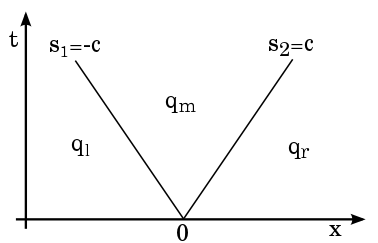
\includegraphics{./figures/acoustics_xt_plane.png}
\caption{Fig 4.1: Structure of the Riemann solution for acoustics.}
\end{figure}

The three constant states are related by the jumps:\\
\begin{align}
q_m = q_\ell + \Delta w_1 r_1 = q_r - \Delta w_2 r_2.
\label{eq:acussol}
\end{align}\\
The jumps in pressure and velocity for each propagating discontinuity
are related in a particular way, since each jump is a multiple of one of
the eigenvectors of \(A\). More generally, the eigenvectors of the
coefficient matrix of a linear hyperbolic system reveal the relation
between jumps in the conserved variables across a wave propagating with
speed given by the corresponding eigenvalue. For acoustics, the
impedance is the physical parameter that determines this relation.

\hypertarget{a-simple-solution}{%
\subsection{A simple solution}\label{a-simple-solution}}

Here we provide some very simple initial data, and determine the Riemann
solution, which consists of three states \(q_\ell\), \(q_m\) and
\(q_r\), and the speeds of the two waves.

    \begin{Verbatim}[fontsize=\small,commandchars=\\\{\}]
{\color{incolor}In [{\color{incolor}7}]:} \PY{c+c1}{\PYZsh{} Initial data for Riemann problem}
        \PY{n}{rho} \PY{o}{=} \PY{l+m+mf}{0.5}               \PY{c+c1}{\PYZsh{} density}
        \PY{n}{bulk} \PY{o}{=} \PY{l+m+mf}{2.}            \PY{c+c1}{\PYZsh{} bulk modulus}
        \PY{n}{ql} \PY{o}{=} \PY{n}{np}\PY{o}{.}\PY{n}{array}\PY{p}{(}\PY{p}{[}\PY{l+m+mi}{3}\PY{p}{,}\PY{l+m+mi}{2}\PY{p}{]}\PY{p}{)}   \PY{c+c1}{\PYZsh{} Left state}
        \PY{n}{qr} \PY{o}{=} \PY{n}{np}\PY{o}{.}\PY{n}{array}\PY{p}{(}\PY{p}{[}\PY{l+m+mi}{3}\PY{p}{,}\PY{o}{\PYZhy{}}\PY{l+m+mi}{2}\PY{p}{]}\PY{p}{)}  \PY{c+c1}{\PYZsh{} Right state}
        \PY{c+c1}{\PYZsh{} Calculated parameters}
        \PY{n}{c} \PY{o}{=} \PY{n}{np}\PY{o}{.}\PY{n}{sqrt}\PY{p}{(}\PY{n}{bulk}\PY{o}{/}\PY{n}{rho}\PY{p}{)}  \PY{c+c1}{\PYZsh{} calculate sound speed}
        \PY{n}{Z} \PY{o}{=} \PY{n}{np}\PY{o}{.}\PY{n}{sqrt}\PY{p}{(}\PY{n}{bulk}\PY{o}{*}\PY{n}{rho}\PY{p}{)}  \PY{c+c1}{\PYZsh{} calculate impedance}
        \PY{n+nb}{print}\PY{p}{(}\PY{l+s+s2}{\PYZdq{}}\PY{l+s+s2}{With density rho = }\PY{l+s+si}{\PYZpc{}g}\PY{l+s+s2}{,  bulk modulus K = }\PY{l+s+si}{\PYZpc{}g}\PY{l+s+s2}{\PYZdq{}} \PYZbs{}
              \PY{o}{\PYZpc{}} \PY{p}{(}\PY{n}{rho}\PY{p}{,}\PY{n}{bulk}\PY{p}{)}\PY{p}{)}
        \PY{n+nb}{print}\PY{p}{(}\PY{l+s+s2}{\PYZdq{}}\PY{l+s+s2}{We compute: sound speed c = }\PY{l+s+si}{\PYZpc{}g}\PY{l+s+s2}{, impedance Z = }\PY{l+s+si}{\PYZpc{}g}\PY{l+s+s2}{ }\PY{l+s+se}{\PYZbs{}n}\PY{l+s+s2}{\PYZdq{}} \PYZbs{}
              \PY{o}{\PYZpc{}} \PY{p}{(}\PY{n}{c}\PY{p}{,}\PY{n}{Z}\PY{p}{)}\PY{p}{)}
\end{Verbatim}

    \begin{Verbatim}[commandchars=\\\{\}]
With density rho = 0.5,  bulk modulus K = 2
We compute: sound speed c = 2, impedance Z = 1 


    \end{Verbatim}

    \begin{Verbatim}[fontsize=\small,commandchars=\\\{\}]
{\color{incolor}In [{\color{incolor}8}]:} \PY{c+c1}{\PYZsh{} Call and print Riemann solution}
        \PY{n}{states}\PY{p}{,} \PY{n}{speeds}\PY{p}{,} \PY{n}{reval} \PY{o}{=} \PYZbs{}
            \PY{n}{acoustics}\PY{o}{.}\PY{n}{exact\PYZus{}riemann\PYZus{}solution}\PY{p}{(}\PY{n}{ql} \PY{p}{,}\PY{n}{qr}\PY{p}{,} \PY{p}{[}\PY{n}{rho}\PY{p}{,} \PY{n}{bulk}\PY{p}{]}\PY{p}{)}
            
        \PY{n+nb}{print}\PY{p}{(}\PY{l+s+s2}{\PYZdq{}}\PY{l+s+s2}{The states ql, qm and qr are: }\PY{l+s+s2}{\PYZdq{}}\PY{p}{)}
        \PY{n+nb}{print}\PY{p}{(}\PY{n}{states}\PY{p}{,} \PY{l+s+s2}{\PYZdq{}}\PY{l+s+se}{\PYZbs{}n}\PY{l+s+s2}{\PYZdq{}}\PY{p}{)}
        \PY{n+nb}{print}\PY{p}{(}\PY{l+s+s2}{\PYZdq{}}\PY{l+s+s2}{The left and right wave speeds are:}\PY{l+s+s2}{\PYZdq{}}\PY{p}{)}
        \PY{n+nb}{print}\PY{p}{(}\PY{n}{speeds}\PY{p}{)}
\end{Verbatim}

    \begin{Verbatim}[commandchars=\\\{\}]
The states ql, qm and qr are: 
[[ 3.  5.  3.]
 [ 2.  0. -2.]] 

The left and right wave speeds are:
[-2.  2.]

    \end{Verbatim}

One way to visualize the Riemann solution for a system of two equations
is by looking at the \(p-u\) phase plane. In the figure below, we show
the two initial conditions of the Riemann problem \(q_\ell\) and \(q_r\)
as points in the phase space; the lines passing through these points
correspond to the eigenvectors, \(r_1\) and \(r_2\).

The middle state \(q_m\) is simply the intersection of the line in the
direction \(r_1\) passing through \(q_\ell\) and the line in the
direction \(r_2\) passing through \(q_r\). The structure of this
solution becomes evident from equation (\ref{eq:acussol}). The dashed
lines correspond to a line in the direction \(r_2\) passing through
\(q_\ell\) and a line in the direction \(r_1\) passing through \(q_r\);
these also intersect, but cannot represent a Riemann solution since they
would involve a wave going to the right but connected to \(q_\ell\) and
a wave going to the left but connected to \(q_r\).

In the live notebook, the cell below allows you to interactively adjust
the initial conditions the material parameters as well as the plot
range, so that you can explore how the structure of the solution in the
phase plane is affected by these quantities.

    \begin{Verbatim}[fontsize=\small,commandchars=\\\{\}]
{\color{incolor}In [{\color{incolor}9}]:} \PY{n}{acoustics\PYZus{}demos}\PY{o}{.}\PY{n}{interactive\PYZus{}phase\PYZus{}plane}\PY{p}{(}\PY{n}{ql}\PY{p}{,}\PY{n}{qr}\PY{p}{,}\PY{n}{rho}\PY{p}{,}\PY{n}{bulk}\PY{p}{)}
\end{Verbatim}

    \begin{center}
    \adjustimage{max size={0.9\linewidth}{0.9\paperheight}}{combined_files/combined_78_0.pdf}
    \end{center}
    { \hspace*{\fill} \\}
    
Note that the eigenvectors are given in terms of the impedance \(Z\),
which depends on the density \(\rho\) and the bulk modulus \(K\).
Therefore, when \(\rho\) and \(K\) are modified the eigenvectors change
and consequently the slope of the lines changes as well.

\hypertarget{examples}{%
\section{Examples}\label{examples}}

We will use the exact solver in {exact\_solvers/acoustics.py} and the
functions in {exact\_solvers/acoustics\_demos.py} to plot interactive
solutions for a few examples.

\hypertarget{shock-tube}{%
\subsection{Shock tube}\label{shock-tube}}

If there is a jump in pressure and the velocity is zero in both initial
states (the shock tube problem) then the resulting Riemann solution
consists of pressure jumps of equal magnitude propagating in both
directions, with equal and opposite jumps in velocity. This is the
linearized version of what is known in fluid dynamics as a shock tube
problem, since it emulates what would happen inside a shock tube, where
the air is initially stationary and a separate chamber at the end of the
tube is pressurized and then released.

    \begin{Verbatim}[fontsize=\small,commandchars=\\\{\}]
{\color{incolor}In [{\color{incolor}10}]:} \PY{n}{ql} \PY{o}{=} \PY{n}{np}\PY{o}{.}\PY{n}{array}\PY{p}{(}\PY{p}{[}\PY{l+m+mi}{5}\PY{p}{,}\PY{l+m+mi}{0}\PY{p}{]}\PY{p}{)}
         \PY{n}{qr} \PY{o}{=} \PY{n}{np}\PY{o}{.}\PY{n}{array}\PY{p}{(}\PY{p}{[}\PY{l+m+mi}{1}\PY{p}{,}\PY{l+m+mi}{0}\PY{p}{]}\PY{p}{)}
         \PY{n}{rho} \PY{o}{=} \PY{l+m+mf}{1.0}
         \PY{n}{bulk} \PY{o}{=} \PY{l+m+mf}{4.0}
         \PY{n}{acoustics\PYZus{}demos}\PY{o}{.}\PY{n}{riemann\PYZus{}plot\PYZus{}pplane}\PY{p}{(}\PY{n}{ql}\PY{p}{,}\PY{n}{qr}\PY{p}{,}\PY{n}{rho}\PY{p}{,}\PY{n}{bulk}\PY{p}{)}
\end{Verbatim}

    \begin{center}
    \adjustimage{max size={0.9\linewidth}{0.9\paperheight}}{combined_files/combined_81_0.pdf}
    \end{center}
    { \hspace*{\fill} \\}
    
    \begin{center}
    \adjustimage{max size={0.9\linewidth}{0.9\paperheight}}{combined_files/combined_81_1.pdf}
    \end{center}
    { \hspace*{\fill} \\}
    
We can also observe the structure of the solution in the phase plane. In
the second plot, we show the structure of the solution in the phase
plane.

\hypertarget{reflection-from-a-wall}{%
\subsection{Reflection from a wall}\label{reflection-from-a-wall}}

As another example, suppose the pressure is initially the same in the
left and right states, while the velocities are non-zero with
\(u_r = -u_\ell > 0\). The flow is converging from both sides and
because of the symmetry of the initial states, the result is a middle
state \(q_m\) in which the velocity is 0 (and the pressure is higher
than on either side).

    \begin{Verbatim}[fontsize=\small,commandchars=\\\{\}]
{\color{incolor}In [{\color{incolor}11}]:} \PY{n}{ql} \PY{o}{=} \PY{n}{np}\PY{o}{.}\PY{n}{array}\PY{p}{(}\PY{p}{[}\PY{l+m+mi}{2}\PY{p}{,}\PY{l+m+mi}{1}\PY{p}{]}\PY{p}{)}  
         \PY{n}{qr} \PY{o}{=} \PY{n}{np}\PY{o}{.}\PY{n}{array}\PY{p}{(}\PY{p}{[}\PY{l+m+mi}{2}\PY{p}{,}\PY{o}{\PYZhy{}}\PY{l+m+mi}{1}\PY{p}{]}\PY{p}{)}  
         \PY{n}{rho} \PY{o}{=} \PY{l+m+mf}{1.0}
         \PY{n}{bulk} \PY{o}{=} \PY{l+m+mf}{1.5}
         \PY{n}{acoustics\PYZus{}demos}\PY{o}{.}\PY{n}{riemann\PYZus{}plot\PYZus{}pplane}\PY{p}{(}\PY{n}{ql}\PY{p}{,}\PY{n}{qr}\PY{p}{,}\PY{n}{rho}\PY{p}{,}\PY{n}{bulk}\PY{p}{)}
\end{Verbatim}

    \begin{center}
    \adjustimage{max size={0.9\linewidth}{0.9\paperheight}}{combined_files/combined_84_0.pdf}
    \end{center}
    { \hspace*{\fill} \\}
    
    \begin{center}
    \adjustimage{max size={0.9\linewidth}{0.9\paperheight}}{combined_files/combined_84_1.pdf}
    \end{center}
    { \hspace*{\fill} \\}
    
We again show the Riemann solution in space and in the phase plane,
where the symmetry is also evident.

Disregarding the left half of the domain (\(x<0\)), one can view this as
a solution to the problem of an acoustic wave impacting a solid wall.
The result is a reflected wave that moves away from the wall; notice
that the velocity vanishes at the wall, as it must. This type of Riemann
solution is important when simulating waves in a domain with reflecting
boundaries. The reflecting condition can be imposed by the use of
fictitious \emph{ghost cells} that lie just outside the domain and whose
state is set by reflecting the interior solution with the symmetry just
described (equal pressure, negated velocity).

In reality, at a material boundary only part of a wave is reflected
while the rest is transmitted. This can be accounted for by including
the spatial variation in \(\rho, K\) and solving a variable-coefficient
Riemann problem.

\hypertarget{interactive-phase-plane-with-solution-at-fixed-time}{%
\subsection{Interactive phase plane with solution at fixed
time}\label{interactive-phase-plane-with-solution-at-fixed-time}}

For a more general exploration of the solution to the acoustics
equation, we now show an interactive solution of the acoustics
equations. The initial states \(q_\ell\) and \(q_r\) can be modified by
dragging and dropping the points in the phase plane plot (in the
notebook version, or on
\hreffoot{http://www.clawpack.org/riemann_book/phase_plane/acoustics_small.html}{this
webpage}).

\hypertarget{gaussian-initial-condition}{%
\subsection{Gaussian initial
condition}\label{gaussian-initial-condition}}

In this example, we use the first example described near the beginning
of this chapter. The initial condition is a Gaussian pressure
perturbation, while the initial velocity is zero. Reflecting boundary
conditions are imposed at \(x=-2\) and \(x=2\), so the wave is fully
reflected back, and we can see how it interacts with itself. This
animation is produced using a numerical method from
\hreffoot{http://www.clawpack.org/pyclaw/}{PyClaw}, and can be viewed in the
interactive notebook or on
\hreffoot{http://www.clawpack.org/riemann_book/html/acoustics_bump_animation.html}{this
webpage}.

\hypertarget{burgers-equation}{%
\chapter{Burgers' equation}\label{burgers-equation}}
\label{sec:04-Burgers}
In this chapter, we study a simple scalar nonlinear conservation law:
Burgers' equation. Burgers' equation models momentum transport in a
fluid of uniform density and pressure, and it is the simplest equation
that captures some key features of gas dynamics or water waves.

To examine the Python code for this chapter, see:

\begin{itemize}
\tightlist
\item
  {exact\_solvers/burgers.py} \ldots{}
  \hreffoot{https://github.com/clawpack/riemann_book/blob/master/exact_solvers/burgers.py}{on
  github,}
\item
  {exact\_solvers/burgers\_demos.py}\ldots{}
  \hreffoot{https://github.com/clawpack/riemann_book/blob/master/exact_solvers/burgers_demos.py}{on
  github.}
\end{itemize}

Burgers' equation has been used extensively for developing both theory
and numerical methods, and it will allow us to explore the Riemann
problem for a nonlinear conservation law. Burgers' equation is a scalar
conservation law with flux \(f(q)=q^2/2\): \begin{align}
q_t + \left(\frac{1}{2}q^2\right)_x = 0.
\label{burgers0}
\end{align} The quasilinear form is obtained by applying the chain rule
to the flux term:\\
\begin{align*}
q_t + qq_x = 0.
\end{align*}\\
This equation looks very similar to the advection equation, with the
difference that the advection speed at each point is given by the
solution \(q\). Burgers' equation is often viewed as a simplified
version of equations in fluid dynamics or water waves that also have
nonlinear fluxes. Our study of the dynamics of equation (\ref{burgers0})
is a step toward understanding these more complex nonlinear systems, in
Chapter \ref{sec:07-Shallow_water} and Chapter \ref{sec:09-Euler}. In
Chapter \ref{sec:05-Traffic_flow} we consider another scalar nonlinear
conservation law that has a similar structure to Burgers' equation and a
simpler physical interpretation.

The \emph{characteristic speed} for Burgers' equation is \(f'(q) = q\).
As long as the solution is smooth, the solution is constant along
characteristic curves \(X(t)\) satisfying \(X'(t) = f'(q(X(t),t)\) since
then \[
\frac{d}{dt} q(X(t),t) = q_x(X(t),t)X'(t) + q_t(X(t),t) = 0.
\] Because of this, the characteristics are straight lines. However,
since the charactistic speed depends on the solution, these lines are
not parallel and characterstics may converge or spread out.

\hypertarget{shock-formation}{%
\section{Shock formation}\label{shock-formation}}

In the figure below we consider Burgers' equation with a Gaussian hump
as the initial data. Since the characteristic speed in Burgers' equation
is given by \(q\) itself, the peak of the hump travels faster than the
rest, and characteristics are converging at the front of the traveling
wave (where \(f'(q)\) decreases with \(x\)) while they are spreading out
behind the peak (where \(f'(q)\) increases with \(x\)). The dashed line
shows the initial condition while the solid lines show the solution at
later times.

    \begin{Verbatim}[fontsize=\small,commandchars=\\\{\}]
{\color{incolor}In [{\color{incolor}5}]:} \PY{n}{interact}\PY{p}{(}\PY{n}{burgers\PYZus{}demos}\PY{o}{.}\PY{n}{multivalued\PYZus{}solution}\PY{p}{,} 
                 \PY{n}{t}\PY{o}{=}\PY{n}{FloatSlider}\PY{p}{(}\PY{n+nb}{min}\PY{o}{=}\PY{l+m+mf}{0.}\PY{p}{,}\PY{n+nb}{max}\PY{o}{=}\PY{l+m+mf}{9.}\PY{p}{,}\PY{n}{value}\PY{o}{=}\PY{l+m+mf}{7.75}\PY{p}{)}\PY{p}{,} \PY{n}{fig}\PY{o}{=}\PY{n}{fixed}\PY{p}{(}\PY{l+m+mi}{0}\PY{p}{)}\PY{p}{)}\PY{p}{;}
\end{Verbatim}

    \begin{center}
    \adjustimage{max size={0.9\linewidth}{0.9\paperheight}}{combined_files/combined_101_0.pdf}
    \end{center}
    { \hspace*{\fill} \\}
    
Notice that at first \(q\) remains single-valued for every \(x\).
However, after some time the crest of the wave overtakes the leading
edge. After this time, we obtain a triple-valued solution for certain
values of \(x\). The first time this overtaking happens is referred to
as the \emph{breaking time} -- a reference to waves breaking on the
beach. It is also the point where the conservation law, in its
differential form, breaks down and where the characteristics cross each
other for the first time. When characteristics cross, a shock wave, or
discontinuity, forms. Mathematically, replacing the triple-valued region
with a discontinuity will avoid the problem of the solution being
multivalued. Where should the shock be located?

If we replace part of the multivalued solution interval with a shock,
some mass will be removed (area \(A_1\) in the figure below) and some
mass will be added (area \(A_2\) in the figure below). In the live
notebook, the figure below shows possible locations for the shock at a
given time; in order to maintain conservation of the integral of \(q\),
the shock must be placed so that these two areas are equal.

    \begin{Verbatim}[fontsize=\small,commandchars=\\\{\}]
{\color{incolor}In [{\color{incolor}6}]:} \PY{n}{interact}\PY{p}{(}\PY{n}{burgers\PYZus{}demos}\PY{o}{.}\PY{n}{shock\PYZus{}location}\PY{p}{,} 
                 \PY{n}{xshock} \PY{o}{=} \PY{n}{FloatSlider}\PY{p}{(}\PY{n+nb}{min}\PY{o}{=}\PY{l+m+mi}{6}\PY{p}{,}\PY{n+nb}{max}\PY{o}{=}\PY{l+m+mi}{10}\PY{p}{,}\PY{n}{step}\PY{o}{=}\PY{l+m+mf}{0.25}\PY{p}{,}\PY{n}{value}\PY{o}{=}\PY{l+m+mf}{7.75}\PY{p}{)}\PY{p}{,}
                 \PY{n}{fig}\PY{o}{=}\PY{n}{fixed}\PY{p}{(}\PY{l+m+mi}{0}\PY{p}{)}\PY{p}{)}\PY{p}{;}
\end{Verbatim}

    \begin{center}
    \adjustimage{max size={0.9\linewidth}{0.9\paperheight}}{combined_files/combined_103_0.pdf}
    \end{center}
    { \hspace*{\fill} \\}
    
This geometric reasoning provides a nice intuition for the shock
location, but is cumbersome in practice. To determine the location of
the shock we can use the \emph{Rankine-Hugoniot jump condition,} which
we will derive in Chapter \ref{sec:05-Traffic_flow}, and which requires
that the jump in flux across a propagating shock must be related to the
jump in \(q\) by \[
s(q_r-q_\ell)  = f(q_r) - f(q_\ell),
\] at each instant in time, where \(s\) is the shock speed at this time.

Since the flux for Burgers' equation is \(f(q) = q^2/2\), this gives
\begin{align*}
s(q_r-q_\ell) & = \frac{1}{2} (q_r^2 - q_\ell^2) \\
\Rightarrow \ \ \ \ s &= \frac{1}{2}(q_\ell + q_r).
\end{align*}\\
In general (as in the image above) the states \(q_\ell\) and \(q_r\)
just to the left and right of the shock will not be constant and the
speed of a shock will change in time.

\hypertarget{shock-solution}{%
\subsection{Shock solution}\label{shock-solution}}

For Burgers' equation, (or any scalar hyperbolic conservation law with a
\emph{convex} flux function, such as the traffic flow problem considered
in Chapter \ref{sec:05-Traffic_flow}), the solution of the Riemann
problem consists of a single wave, which may be either a shock or a
rarefaction, separating regions of constant value \(q_\ell\) and
\(q_r\). Here convexity of the flux \(f(q)\) means that \(f'(q)\) is
either monotonically increasing or monotonically decreasing as \(q\)
varies. If \(f(q)\) is not convex then the solution can be more
complicated; see the section on Convexity below and in
Chapter \ref{sec:06-Nonconvex_scalar}.

The analysis above already yields the solution to the Riemann problem in
the case that the resulting wave is a shock. The entropy condition, as
we will explain below, indicates that a shock will form when
\(f'(q_\ell) > f'(q_r)\); i.e.~when \(q_\ell>q_r\). In this case, the
solution is \begin{align*}
q(x,t) = 
\begin{cases}
q_\ell \quad \text{if} \ \ x/t<s \\
q_r \quad \text{if} \ \ x/t>s.
\end{cases}
\end{align*}\\
Below, we plot the solution of Burgers' equation for an initial
condition that leads to a shock (i.e.~with \(q_\ell>q_r\)).

    \begin{Verbatim}[fontsize=\small,commandchars=\\\{\}]
{\color{incolor}In [{\color{incolor}7}]:} \PY{n}{interact}\PY{p}{(}\PY{n}{burgers\PYZus{}demos}\PY{o}{.}\PY{n}{shock}\PY{p}{(}\PY{p}{)}\PY{p}{,} 
                 \PY{n}{t}\PY{o}{=}\PY{n}{widgets}\PY{o}{.}\PY{n}{FloatSlider}\PY{p}{(}\PY{n+nb}{min}\PY{o}{=}\PY{l+m+mi}{0}\PY{p}{,}\PY{n+nb}{max}\PY{o}{=}\PY{l+m+mf}{1.0}\PY{p}{,}\PY{n}{value}\PY{o}{=}\PY{l+m+mf}{0.5}\PY{p}{)}\PY{p}{,}
                 \PY{n}{which\PYZus{}char}\PY{o}{=}\PY{n}{widgets}\PY{o}{.}\PY{n}{Checkbox}\PY{p}{(}\PY{n}{value}\PY{o}{=}\PY{k+kc}{True}\PY{p}{,}
                                             \PY{n}{description}\PY{o}{=}\PY{l+s+s1}{\PYZsq{}}\PY{l+s+s1}{Show characteristics}\PY{l+s+s1}{\PYZsq{}}\PY{p}{)}\PY{p}{)}\PY{p}{;}
\end{Verbatim}

    \begin{center}
    \adjustimage{max size={0.9\linewidth}{0.9\paperheight}}{combined_files/combined_106_0.pdf}
    \end{center}
    { \hspace*{\fill} \\}
    
\hypertarget{rarefaction-wave}{%
\section{Rarefaction wave}\label{rarefaction-wave}}

In the previous figure with the hump as the initial condition, we
observed that a shock formed on the right side of the hump. However, on
the left side, the characteristics spread out and will never cross. This
part of the solution is called a rarefaction wave. This is the kind of
behavior we will observe in the solution of the Riemann problem when
\(q_\ell<q_r\).

In the next figure, we consider such a Riemann problem. Although the
initial data is discontinuous at \(x=0\), we can think of smearing it
out slightly to a continuous function so that all values between
\(q_\ell\) and \(q_r\) are taken over a very narrow region around
\(x=0\). As time evolves, each value of \(q\) propagates according to
the advection speed \(q\) given by the quasi-linear equation. Therefore,
after time \(t\), each value \(q\) must propagate a distance \(x=qt\),
so the solution along the rarefaction is then \(q = x/t\). As
\(q_\ell<q_r\), the smallest and largest displacements are given by
\(q_\ell t\) and \(q_r t\), respectively.

    \begin{Verbatim}[fontsize=\small,commandchars=\\\{\}]
{\color{incolor}In [{\color{incolor}8}]:} \PY{n}{interact}\PY{p}{(}\PY{n}{burgers\PYZus{}demos}\PY{o}{.}\PY{n}{rarefaction\PYZus{}figure}\PY{p}{,} 
                 \PY{n}{t} \PY{o}{=} \PY{n}{FloatSlider}\PY{p}{(}\PY{n+nb}{min}\PY{o}{=}\PY{l+m+mi}{0}\PY{p}{,}\PY{n+nb}{max}\PY{o}{=}\PY{l+m+mi}{9}\PY{p}{,}\PY{n}{value}\PY{o}{=}\PY{l+m+mi}{5}\PY{p}{)}\PY{p}{)}\PY{p}{;}
\end{Verbatim}

    \begin{center}
    \adjustimage{max size={0.9\linewidth}{0.9\paperheight}}{combined_files/combined_108_0.pdf}
    \end{center}
    { \hspace*{\fill} \\}
    
The full rarefaction solution for the Burgers' Riemann problem is then
simply given by \begin{align*}
q(x,t) = 
\begin{cases}
q_\ell, \quad \text{for} \ \ x<q_\ell t \\
x/t, \quad \text{for} \ \ q_\ell t \le x \le q_r t \\
q_r, \quad \text{for} \ \ x>q_r t.
\end{cases}
\end{align*}

As we will see in Chapter \ref{sec:05-Traffic_flow}, the rarefaction
solution is always a self-similar solution. This means that it can be
expressed as a function of the ratio between position and time
\(q(x,t) = \tilde{q}(x/t)\), so it remains the same when rescaling both
\(x\) and \(t\) by the same factor. In Burgers' equation, the form of
the rarefaction is particularly simple since the advection speed is
simply \(q\) and so the rarefaction wave is linear in \(x\) with slope
\(1/t\) at time \(t\).

\hypertarget{rarefaction-solution}{%
\subsection{Rarefaction solution}\label{rarefaction-solution}}

In the figure below, we plot a solution of the Riemann problem with
\(q_\ell<q_r\), exhibiting a rarefaction.

    \begin{Verbatim}[fontsize=\small,commandchars=\\\{\}]
{\color{incolor}In [{\color{incolor}9}]:} \PY{n}{interact}\PY{p}{(}\PY{n}{burgers\PYZus{}demos}\PY{o}{.}\PY{n}{rarefaction}\PY{p}{(}\PY{p}{)}\PY{p}{,} 
                 \PY{n}{t}\PY{o}{=}\PY{n}{widgets}\PY{o}{.}\PY{n}{FloatSlider}\PY{p}{(}\PY{n+nb}{min}\PY{o}{=}\PY{l+m+mi}{0}\PY{p}{,}\PY{n+nb}{max}\PY{o}{=}\PY{l+m+mf}{1.0}\PY{p}{,}\PY{n}{value}\PY{o}{=}\PY{l+m+mf}{0.5}\PY{p}{)}\PY{p}{,}
                 \PY{n}{which\PYZus{}char}\PY{o}{=}\PY{n}{widgets}\PY{o}{.}\PY{n}{Checkbox}\PY{p}{(}\PY{n}{value}\PY{o}{=}\PY{k+kc}{True}\PY{p}{,}
                                             \PY{n}{description}\PY{o}{=}\PY{l+s+s1}{\PYZsq{}}\PY{l+s+s1}{Show characteristics}\PY{l+s+s1}{\PYZsq{}}\PY{p}{)}\PY{p}{)}\PY{p}{;}
\end{Verbatim}

    \begin{center}
    \adjustimage{max size={0.9\linewidth}{0.9\paperheight}}{combined_files/combined_111_0.pdf}
    \end{center}
    { \hspace*{\fill} \\}
    
\hypertarget{weak-solutions}{%
\section{Weak solutions}\label{weak-solutions}}

As we mentioned before, the differential form of the equation breaks
down in the presence of shocks/discontinuities. However, the integral
form of the conservation law remains valid. Let's integrate the general
conservation law \(q_t+f(q)_x=0\) from \(x=x_1\) to \(x=x_2\) and
\(t=t_1\) to \(t=t_2\): \begin{align*}
\int_{t_1}^{t_2}\int_{x_1}^{x_2} [q_t+f(q)_x] dx dt = 0.
\end{align*} This integral can be rewritten in terms of an indicator
function \(\phi(x,t)\) in \([x_1,x_2]\times[t_1,t_2]\) (defined to be 1
in this region, zero elsewhere): \begin{align}
\int_{0}^{\infty}\int_{-\infty}^{\infty} [q_t+f(q)_x]\phi(x,t) dx dt = 0.
\label{eq:Burgersintclaw2}
\end{align}

We can further replace \(\phi(x,t)\) by a smooth function with compact
support on some region of the \(x-t\) plane (zero outside a closed and
bounded region). Assuming \(t=0\) is in the support of \(\phi(x,t)\),
integration by parts yields \begin{align}
\int_{0}^{\infty}\int_{-\infty}^{\infty} [q\phi_t+f(q)\phi_x] dx dt = -\int_{-\infty}^{\infty}q(x,0)\phi(x,0)dx,
\label{eq:Burgersintclaw3}
\end{align} where now the derivatives are on \(\phi(x,t)\) and not on
\(q\) or \(f(q)\), so the equation still makes sense for discontinuous
\(q\). Note that we only obtain one boundary term along \(t=0\) since
\(\phi(x,t)\) vanishes at infinity. The function \(q(x,t)\) is called a
\emph{weak solution} of the conservation law if
(\ref{eq:Burgersintclaw3}) holds for all functions \(\phi(x,t)\) that
are continuously differentiable and have compact support (bump
functions). However, the function \(\phi(x,t)\) chosen in
(\ref{eq:Burgersintclaw2}) does not satisfy these conditions since it is
not smooth. Nonetheless, we can approximate this function arbitrarily
well by a smooth function. Note that any weak solution is a solution of
the integral conservation law and vice versa.

Weak solutions are thus allowed to include discontinuities. The shock
solution presented above, for instance, is a weak solution of Burgers'
equation. After characteristics cross, there is no strong solution of
the conservation law, and we must resort to weak solutions.

\hypertarget{an-unphysical-weak-solution}{%
\subsection{An unphysical weak
solution}\label{an-unphysical-weak-solution}}

A potential problem with the notion of weak solutions is that in some
cases the weak solution is not unique. For example, consider the Riemann
problem for Burgers' equation with \(q_\ell < q_r\). As mentioned
already we expect a rarefaction to be the correct solution. This is
because if we smeared out the initial data just slightly then there
would be smoothly varying characteristics emerging from each point \(x\)
and these characteristics would spread out. However, for exactly
discontinuous initial data, there exists another weak solution in which
the initial discontinuity propagates as a shock wave with the
Rankine-Hugoniot speed \((q_\ell + q_r)/2\): \begin{align*}
q(x,t) = 
\begin{cases}
q_\ell \quad \text{if} \ \ x/t<s \\
q_r \quad \text{if} \ \ x/t>s.
\end{cases}
\end{align*} This unphysical solution is also referred to as an
expansion shock, and it is also a weak solution to Burgers' equation. In
the next figure, we plot this weak solution.

    \begin{Verbatim}[fontsize=\small,commandchars=\\\{\}]
{\color{incolor}In [{\color{incolor}10}]:} \PY{n}{interact}\PY{p}{(}\PY{n}{burgers\PYZus{}demos}\PY{o}{.}\PY{n}{unphysical}\PY{p}{(}\PY{p}{)}\PY{p}{,} 
                  \PY{n}{t}\PY{o}{=}\PY{n}{widgets}\PY{o}{.}\PY{n}{FloatSlider}\PY{p}{(}\PY{n+nb}{min}\PY{o}{=}\PY{l+m+mi}{0}\PY{p}{,}\PY{n+nb}{max}\PY{o}{=}\PY{l+m+mf}{1.0}\PY{p}{,}\PY{n}{value}\PY{o}{=}\PY{l+m+mf}{0.5}\PY{p}{)}\PY{p}{,}
                  \PY{n}{which\PYZus{}char}\PY{o}{=}\PY{n}{widgets}\PY{o}{.}\PY{n}{Checkbox}\PY{p}{(}\PY{n}{value}\PY{o}{=}\PY{k+kc}{True}\PY{p}{,}
                                              \PY{n}{description}\PY{o}{=}\PY{l+s+s1}{\PYZsq{}}\PY{l+s+s1}{Show characteristics}\PY{l+s+s1}{\PYZsq{}}\PY{p}{)}\PY{p}{)}\PY{p}{;}
\end{Verbatim}

    \begin{center}
    \adjustimage{max size={0.9\linewidth}{0.9\paperheight}}{combined_files/combined_115_0.pdf}
    \end{center}
    { \hspace*{\fill} \\}
    
Note the behavior of the characteristics with respect to the shock. The
fact that the characteristics are spreading away from the shock rather
than converging on it indicates that the correct solution should instead
be a rarefaction. In order to be able to specify which of the weak
solutions is physically correct, we need to derive a mathematical
condition from our physical intuition gained from observing the behavior
of the characteristics. This condition is referred to as the entropy
condition.

\hypertarget{the-entropy-condition}{%
\subsection{The entropy condition}\label{the-entropy-condition}}

A given initial value problem for a hyperbolic PDE may have many weak
solutions. A condition that selects a unique physically correct solution
out of these weak solutions is called an \emph{admissibility condition}
or more often an \emph{entropy condition}. This name comes from gas
dynamics, where the physical entropy must increase in the gas passing
through a shock, according to the second law of thermodynamics. A
discontinuity that violates this is non-physical. A mathematical
``entropy function'' with a similar property can often be defined for
other conservation laws. More discussion of this and several other
formulations of admissibility conditions, with more detailed
explanations, are available in the literature, for example in many of
the books cited in the Chapter \ref{sec:00-Preface}.

In the context of the Riemann problem, the entropy condition allows us
to determine if the physical solution should involve a shock or a
rarefaction. In the case of scalar conservation laws, the entropy
condition is quite simple and can be formulated in terms of the flux
function of the conservation law as follows: the solution of a scalar
Riemann problem will consist of a shock only if \[
f'(q_\ell) > f'(q_r).
\] In other words, the solution is a shock only if nearby
characteristics from the left and right approach the shock as time
progresses. This is often called the \emph{Lax Entropy Condition}. If
nearby characteristics are spreading out, as in the last example, the
correct solution is instead a rarefaction. In the case of Burgers'
equation, the flux function is \(f(q)=q^2/2\), so the correct solution
is a shock only if \[
q_\ell > q_r,
\] which can be clearly observed in the interactive solution below (in
the notebook). In later chapters, we will see how this condition
generalizes to systems of conservation laws.

\hypertarget{convexity}{%
\subsection{Convexity}\label{convexity}}

The flux \(f(q) = q^2/2\) for Burgers' equation is a convex function,
since \(f''(q) = 1 > 0\) for all values of \(q\). This means that as
\(q\) varies between \(q_\ell\) and \(q_r\) the the characteristic speed
\(f'(q) = q\) is either monotonically increasing (if \(q_\ell < q_r\))
or monotonically decreasing (if \(q_\ell > q_r\)). Hence for any Riemann
problem the characteristic speeds for intermediate states are either
purely converging or purely diverging, and the Riemann solution is
always either a single rarefaction wave or a single shock wave.

The flux \(f(\rho) = \rho(1-\rho)\) of the simple traffic flow model
that we will consider in Chapter \ref{sec:05-Traffic_flow} also has the
property that \(f'(\rho)\) varies monotonically with \(\rho\) (in the
context of hyperbolic PDEs, a flux function is referred to as
\emph{convex} if either \(f''(q)\ge0\) for all \(q\) or \(f''(q)\le 0\)
for all \(q\)). Since \(f''\) is always negative for the traffic flow
model, the correct Riemann solution is a shock if
\(\rho_\ell < \rho_r\), or a rarefaction wave if \(\rho_\ell > \rho_r\).

The solution to the Riemann problem can be much more complicated if
\(f'(q)\) is not monotonically varying between \(q_\ell\) and \(q_r\),
i.e.~if \(f''(q)\) changes sign. In this case the Riemann solution can
consist of multiple shock and rarefaction waves. The nonconvex case is
explored further in Chapter \ref{sec:06-Nonconvex_scalar}.

\hypertarget{interactive-solution-and-examples}{%
\section{Interactive solution and
examples}\label{interactive-solution-and-examples}}

In the live notebook, the figure below is an interactive solution of the
Riemann problem for Burgers' equation. The values of the initial
conditions and the time can be modified to observe their effect on the
characteristic structure and the solution.

\hypertarget{animations-of-more-complex-solutions}{%
\section{Animations of more complex
solutions}\label{animations-of-more-complex-solutions}}

We can now explore a few more examples that are representative of
phenomena we will observe in more complicated systems, with more
interesting initial data that the single jump discontinuity of a Riemann
problem. For the animations shown below, the solution is computed
numerically using \hreffoot{http://www.clawpack.org/pyclaw/}{PyClaw}.

\hypertarget{bump-initial-conditions}{%
\subsection{Bump initial conditions}\label{bump-initial-conditions}}

The animation below in the notebook, or on
\hreffoot{http://www.clawpack.org/riemann_book/html/burgers_animation0.html}{this
webpage}, shows the solution of Burgers' equation for an initial
Gaussian hump, as discussed at the beginning of this chapter. A shock
forms on the leading edge and the trailing edge spreads out as a
rarefaction.

\hypertarget{three-state-data-with-merging-shocks}{%
\subsection{Three-state data with merging
shocks}\label{three-state-data-with-merging-shocks}}

For an initial condition that is piecewise-constant with three values,
one can solve Burgers' equation by solving a Riemann problem locally for
each discontinuity and then considering how the resulting waves
interact. For instance, consider the initial condition \begin{align*}
q_0(x) = 
\begin{cases}
q_\ell \quad \text{if} \ \ x < -1 \\
q_m \quad \text{if} \ \ -1\le x \le 1 \\
q_r \quad \text{if} \ \ x > 1.
\end{cases}
\end{align*}\\
We can decompose this into two Riemann problems: one at \(x=-1\) and
another at \(x=1\). Each of these two Riemann problems will yield either
a shock or a rarefaction. The interesting part is what happens when the
generated shocks or rarefactions interact. In the scenario shown below,
let us assume that both Riemann problems produce a right-propagating
shock. However, the shock generated at \(x=-1\) propagates faster, so it
will eventually reach the shock originally generated at \(x=1\). At the
point in time when the shocks collide, one can simply restate the
problem again as a Riemann problem and solve the whole problem
analytically. In this animation, the plot on the left shows the solution
\(q(x)\) evolving through time, while the one on the right shows the
characteristic structure in the \(x-t\) plane, with the shocks shown as
wide lines and the characteristics as thin lines, and with time is
marked by a horizontal dashed line. In this animation, one can clearly
see the two shocks merge to become a single shock at later times. This
animation can be viewed in the live notebook on or
\hreffoot{http://www.clawpack.org/riemann_book/html/burgers_animation1.html}{this
webpage}.

\hypertarget{three-state-data-with-interacting-shock-and-rarefaction}{%
\subsection{Three-state data with interacting shock and
rarefaction}\label{three-state-data-with-interacting-shock-and-rarefaction}}

As one would expect, this can become more complicated when one or both
of the waves generated are given by rarefactions. The animation below,
or on
\hreffoot{http://www.clawpack.org/riemann_book/html/burgers_animation2.html}{this
webpage}, shows how a right-propagating shock can overtake a
rarefaction. The shock speed changes as it passes through the
rarefaction, since the state just to the left of the shock is changing.
This is seen clearly in the \(x-t\) plane, where the slope of the shock
is changed after interacting with the rarefaction. Note the shock is
again marked as a wider line.

Analogously, one can also have a rarefaction overtaking a shock. As seen
in the animation below, or
\hreffoot{http://www.clawpack.org/riemann_book/html/burgers_animation3.html}{this
webpage}, this can even change the direction in which the shock is
propagating. This happens because the velocity of the shock depends on
the slopes of the impinging characteristics. When a shock interacts with
a rarefaction, the varying slopes of the characteristic curves produce a
constant change of the shock propagation velocity.

In the notebook, try modifying the values of \(q_\ell\), \(q_m\) and
\(q_r\) in order to see what other behavior can be observed. Is it
possible to observe two interacting rarefactions?

\hypertarget{traffic-flow-the-lighthill-whitham-richards-model}{%
\chapter{Traffic flow: the Lighthill-Whitham-Richards
model}\label{traffic-flow-the-lighthill-whitham-richards-model}}
\label{sec:05-Traffic_flow}
In this chapter we investigate a conservation law that models the flow
of traffic. This model is sometimes referred to as the
Lighthill-Whitham-Richards (or LWR) traffic model (see
\cite{lighthill1955kinematic} and \cite{richards1956shock}). This model
and the corresponding Riemann problem are discussed in many places; the
discussion here is most closely related to that in Chapter 11 of
\cite{fvmhp}.

This nonlinear scalar problem is similar to Burgers' equation that we
already discussed in Chapter \ref{sec:04-Burgers} in many ways, since
both involve a quadratic (and hence convex) flux function. In this
notebook we repeat some of the discussion from
Chapter \ref{sec:04-Burgers} in order to reinforce essential concepts
that will be important throughout the remainder of the book.

If you wish to examine the Python code for this chapter, please see:

\begin{itemize}
\tightlist
\item
  {exact\_solvers/traffic\_LWR.py} \ldots{}
  \hreffoot{https://github.com/clawpack/riemann_book/blob/master/exact_solvers/traffic_LWR.py}{on
  github,}
\item
  {exact\_solvers/traffic\_demos.py} \ldots{}
  \hreffoot{https://github.com/clawpack/riemann_book/blob/master/exact_solvers/traffic_demos.py}{on
  github.}
\end{itemize}

\hypertarget{the-lwr-model}{%
\section{The LWR model}\label{the-lwr-model}}

Recall the continuity equation for any density that is advected with a
flow: \[\rho_t + (u\rho)_x = 0.\]\\
In this chapter, \(\rho\) represents the density of cars on a road,
traveling with velocity \(u\). Note that we're not keeping track of the
individual cars, but just of the average number of cars per unit length
of road. Thus \(\rho=0\) represents an empty stretch of road, and we can
choose the units so that \(\rho=1\) represents bumper-to-bumper traffic.

We'll also choose units so that the speed limit is \(u_\text{max}=1\),
and assume that drivers never go faster than this (yeah, right!). If we
assume that drivers always travel at a single uniform velocity, we
obtain once again the advection equation that we studied in
Chapter \ref{sec:02-Advection}. But we all know that's not accurate in
practice -- cars go faster in light traffic and slower when there is
congestion. The simplest way to incorporate this effect is to make the
velocity a linearly decreasing function of the density:
\[u(\rho) = 1 - \rho.\] Notice that \(u\) goes to zero as \(\rho\)
approaches the maximum density of 1, while \(u\) goes to the maximum
value of 1 as traffic density goes to zero. Obviously, both \(\rho\) and
\(u\) should always stay in the interval \([0,1]\).

Here is a plot of this velocity function:

    \begin{Verbatim}[fontsize=\small,commandchars=\\\{\}]
{\color{incolor}In [{\color{incolor}3}]:} \PY{n}{Image}\PY{p}{(}\PY{l+s+s1}{\PYZsq{}}\PY{l+s+s1}{figures/LWR\PYZhy{}Velocity.png}\PY{l+s+s1}{\PYZsq{}}\PY{p}{,} \PY{n}{width}\PY{o}{=}\PY{l+m+mi}{350}\PY{p}{)}
\end{Verbatim}
\texttt{\color{outcolor}Out[{\color{outcolor}3}]:}
    
    \begin{center}
    \adjustimage{max size={0.9\linewidth}{0.9\paperheight}}{combined_files/combined_137_0.png}
    \end{center}
    { \hspace*{\fill} \\}
    

Combining the two equations above, our conservation law says
\[\rho_t + (\rho (1-\rho))_x = 0\] with the flux function
\[f(\rho) = \rho(1-\rho)\] giving the rate of flow of cars. Notice how
the flux is zero when there are no cars (\(\rho=0\)) and also when the
road is completely full (\(\rho=1\)). The maximum flow of traffic
actually occurs when the road is half full, as the plot below shows.

    \begin{Verbatim}[fontsize=\small,commandchars=\\\{\}]
{\color{incolor}In [{\color{incolor}4}]:} \PY{n}{f} \PY{o}{=} \PY{k}{lambda} \PY{n}{rho}\PY{p}{:} \PY{n}{rho}\PY{o}{*}\PY{p}{(}\PY{l+m+mi}{1}\PY{o}{\PYZhy{}}\PY{n}{rho}\PY{p}{)}
        \PY{n}{traffic\PYZus{}demos}\PY{o}{.}\PY{n}{plot\PYZus{}flux}\PY{p}{(}\PY{n}{f}\PY{p}{)}
\end{Verbatim}

    \begin{center}
    \adjustimage{max size={0.9\linewidth}{0.9\paperheight}}{combined_files/combined_139_0.pdf}
    \end{center}
    { \hspace*{\fill} \\}
    
Like the flux in Bugers' equation, the LWR flux is \textbf{nonlinear},
so we again expect to see shock waves and rarefaction waves in the
solution. We can superficially make this equation look like the
advection equation by using the chain rule to write it in quasilinear
form:\\
\[f(\rho)_x = f'(\rho) \rho_x = (1-2\rho)\rho_x.\]\\
Then we have\\
\[\rho_t + (1-2\rho)\rho_x = 0.\]\\
This is like the advection equation, but with a velocity \(1-2\rho\)
that depends on the density of cars. The value \(f'(\rho)=1-2\rho\) is
referred to as the \emph{characteristic speed}. This characteristic
speed is not the speed at which cars move (notice that it can even be
negative, whereas cars only drive to the right in our model) Rather, it
is the speed at which \emph{information} is transmitted along the road.
Notice that the LWR flux is not convex but concave; because of this, the
characteristic speed is a decreasing function of the density.

\hypertarget{example-traffic-jam}{%
\section{Example: Traffic jam}\label{example-traffic-jam}}

What does our model predict when traffic approaches a totally congested
(\(\rho=1\)) area? This might be due to construction, an accident or a
red light somewhere to the right; upstream of the obstruction, cars will
be bumper-to-bumper, so we set \(\rho=1\) for \(x>0\) (supposing that
traffic has backed up to that point). For \(x<0\) we'll assume a lower
density \(\rho_\ell<1\). This is another example of a Riemann problem:
two constant states separated by a discontinuity. We have\\
\[
\rho(x,t=0) = \begin{cases} \rho_\ell & x<0 \\
                            1 & x>0. \end{cases}
\]\\
What will happen as time goes forward? Intuitively, we expect traffic to
continue backing up to the left, so the region with \(\rho=1\) will
extend further and further to the left. This corresponds to the
discontinuity (or shock wave) moving to the left. How quickly will it
move? The example below shows the solution (on the left) and individual
vehicle trajectories in the \(x-t\) plane (on the right).

    \begin{Verbatim}[fontsize=\small,commandchars=\\\{\}]
{\color{incolor}In [{\color{incolor}5}]:} \PY{n}{interact}\PY{p}{(}\PY{n}{traffic\PYZus{}demos}\PY{o}{.}\PY{n}{jam}\PY{p}{,} 
                 \PY{n}{rho\PYZus{}l}\PY{o}{=}\PY{n}{FloatSlider}\PY{p}{(}\PY{n+nb}{min}\PY{o}{=}\PY{l+m+mf}{0.1}\PY{p}{,}\PY{n+nb}{max}\PY{o}{=}\PY{l+m+mf}{0.9}\PY{p}{,}\PY{n}{value}\PY{o}{=}\PY{l+m+mf}{0.5}\PY{p}{,}
                                   \PY{n}{description}\PY{o}{=}\PY{l+s+sa}{r}\PY{l+s+s1}{\PYZsq{}}\PY{l+s+s1}{\PYZdl{}}\PY{l+s+s1}{\PYZbs{}}\PY{l+s+s1}{rho\PYZus{}l\PYZdl{}}\PY{l+s+s1}{\PYZsq{}}\PY{p}{)}\PY{p}{,}
                 \PY{n}{t}\PY{o}{=}\PY{n}{FloatSlider}\PY{p}{(}\PY{n+nb}{min}\PY{o}{=}\PY{l+m+mf}{0.}\PY{p}{,}\PY{n+nb}{max}\PY{o}{=}\PY{l+m+mf}{1.}\PY{p}{,}\PY{n}{value}\PY{o}{=}\PY{l+m+mf}{0.5}\PY{p}{)}\PY{p}{,} \PY{n}{fig}\PY{o}{=}\PY{n}{fixed}\PY{p}{(}\PY{l+m+mi}{0}\PY{p}{)}\PY{p}{)}\PY{p}{;}
\end{Verbatim}

    \begin{center}
    \adjustimage{max size={0.9\linewidth}{0.9\paperheight}}{combined_files/combined_142_0.pdf}
    \end{center}
    { \hspace*{\fill} \\}
    
Note that the vehicle trajectory plot above shows the motion of cars
moving at velocity \(u_\ell = 1 - \rho_\ell>0\) as they approach the
traffic jam, and at speed \(u_r = 1-\rho_r = 0\) to the right of the
shock, where the cars are stationary.

Unlike the case of linear advection, the \emph{characteristic speeds}
are different, with \(f'(\rho_\ell) = 1 - 2\rho_\ell\), which could be
either negative or positive depending on \(\rho_\ell\), and
\(f'(\rho_r) = -1\).

\hypertarget{speed-of-a-shock-wave-the-rankine-hugoniot-condition}{%
\section{Speed of a shock wave: the Rankine-Hugoniot
condition}\label{speed-of-a-shock-wave-the-rankine-hugoniot-condition}}

In the plot above, we see a shock wave (i.e., a discontinuity) that
moves to the left as more and more cars pile up behind the traffic jam.
How quickly does this discontinuity move to the left?

We can figure it out by putting an imaginary line at the location of the
shock, as shown in the next figure.

Let \(\rho_\ell\) be the density of cars just to the left of the line,
and let \(\rho_r\) be the density of cars just to the right. Imagine for
a moment that the line is stationary. Then the rate of cars reaching the
line from the left is \(f(\rho_\ell)\) and the rate of cars departing
from the line to the right is \(f(\rho_r)\). If the line really were
stationary, we would need to have \(f(\rho_\ell)-f(\rho_r)=0\) to avoid
cars accumulating at the line.

    \begin{Verbatim}[fontsize=\small,commandchars=\\\{\}]
{\color{incolor}In [{\color{incolor}6}]:} \PY{n}{Image}\PY{p}{(}\PY{l+s+s1}{\PYZsq{}}\PY{l+s+s1}{figures/shock\PYZus{}diagram\PYZus{}traffic\PYZus{}a.png}\PY{l+s+s1}{\PYZsq{}}\PY{p}{,} \PY{n}{width}\PY{o}{=}\PY{l+m+mi}{350}\PY{p}{)}
\end{Verbatim}
\texttt{\color{outcolor}Out[{\color{outcolor}6}]:}
    
    \begin{center}
    \adjustimage{max size={0.9\linewidth}{0.9\paperheight}}{combined_files/combined_146_0.png}
    \end{center}
    { \hspace*{\fill} \\}
    

However, the shock is not stationary, so the line is moving. Let \(s\)
be the speed of the shock. Then as the line moves to the left, some cars
that were to the left are now to the right of the line. The rate of cars
removed from the left is \(s \rho_\ell\) and the rate of cars added on
the right is \(s \rho_r\), as shown in this figure:

    \begin{Verbatim}[fontsize=\small,commandchars=\\\{\}]
{\color{incolor}In [{\color{incolor}7}]:} \PY{n}{Image}\PY{p}{(}\PY{l+s+s1}{\PYZsq{}}\PY{l+s+s1}{figures/shock\PYZus{}diagram\PYZus{}traffic\PYZus{}b.png}\PY{l+s+s1}{\PYZsq{}}\PY{p}{,} \PY{n}{width}\PY{o}{=}\PY{l+m+mi}{350}\PY{p}{)}
\end{Verbatim}
\texttt{\color{outcolor}Out[{\color{outcolor}7}]:}
    
    \begin{center}
    \adjustimage{max size={0.9\linewidth}{0.9\paperheight}}{combined_files/combined_148_0.png}
    \end{center}
    { \hspace*{\fill} \\}
    

So in order to avoid an infinite density of cars at the shock, these two
effects need to be balanced:

\[f(\rho_\ell) - f(\rho_r) = s(\rho_\ell - \rho_r).\]

This same condition was used for Burgers' equation in
Chapter \ref{sec:04-Burgers}, and is known as the
\textbf{Rankine-Hugoniot condition}. It holds for any shock wave in the
solution of any hyperbolic PDE (even systems of equations, where the
corresponding vector version gives even more information about the
structure of allowable shock waves).

Returning to our traffic jam scenario, we set \(\rho_r=1\). Then we find
that the Rankine-Hugoniot condition gives the shock speed
\[s = \frac{f(\rho_\ell)-f(\rho_r)}{\rho_\ell-\rho_r} = \frac{f(\rho_\ell)}{\rho_\ell-1} =  -\rho_\ell.\]
This makes sense: the traffic jam propagates back along the road, and it
does so more quickly if there is a greater density of approaching cars.

\hypertarget{example-green-light}{%
\section{Example: green light}\label{example-green-light}}

What about when a traffic light turns green? At \(t=0\), when the light
changes, there will be a discontinuity, with traffic backed up behind
the light but little or no traffic after the light. With the light at
\(x=0\), this takes the form of another Riemann problem:\\
\[
\rho(x,t=0) = \begin{cases} 1 & x<0, \\
                            \rho_r & x>0, \end{cases}
\]\\
with \(\rho_r = 0\), for example. In this case we don't expect the
discontinuity in density to propagate. Physically, the reason is clear:
after the light turns green, the cars in front accelerate and spread
out; then the cars behind them accelerate, and so forth. This kind of
expansion wave is referred to as a \emph{rarefaction wave} because the
drivers experience a decrease in density (a rarefaction) as they pass
through this wave. Initially, the solution is discontinuous, but after
time zero it becomes continuous.

\hypertarget{similarity-solutions}{%
\subsection{Similarity solutions}\label{similarity-solutions}}

The exact form of the solution at a green light can be determined by
assuming that the solution \(\rho(x,t)\) depends only on \(x/t\). A
solution with this property is referred to as a \emph{similarity
solution} because it remains the same if we rescale both \(x\) and \(t\)
by the same factor. The solution of any Riemann problem is, in fact, a
similarity solution. Writing \(\rho(x,t) = \tilde{\rho}(x/t)\) we have
(with \(\xi = x/t\)):\\
\begin{align*}
    \rho_t & = -\frac{x}{t^2}\tilde{\rho}'(\xi) & f(\rho)_x & = \frac{1}{t}\tilde{\rho}'(\xi) f'(\tilde{\rho}(\xi)).
\end{align*}\\
Thus\\
\begin{align}
    \rho_t + f(\rho)_x = -\frac{x}{t^2}\tilde{\rho}'(\xi) + \frac{1}{t}\tilde{\rho}'(\xi) f'(\tilde{\rho}(\xi)) = 0.
\end{align}\\
This can be solved to find \begin{align}
    f'(\tilde{\rho}(\xi)) & = \frac{x}{t}
\end{align}\\
or, since \(f'(\tilde{\rho}) = 1-2\tilde{\rho}\),\\
\begin{align}
    \tilde{\rho}(\xi) & = \frac{1}{2}\left(1 - \frac{x}{t}\right).
\end{align}\\
We know that the solution far enough to the left is just
\(\rho_\ell=1\), and far enough to the right it is \(\rho_r\). The
formula above gives the solution in the region between these constant
states. For instance, if \(\rho_r=0\) (i.e., the road beyond the light
is empty at time zero), then\\
\begin{align}
\rho(x,t) & = \begin{cases}
                1 & x/t \le -1 \\
                \frac{1}{2}\left(1 - x/t\right) & -1 < x/t < 1 \\
                0 & 1 \le x/t.
            \end{cases}
\end{align}

The plot below shows the solution density and vehicle trajectories for a
green light at \(x=0\).

    \begin{Verbatim}[fontsize=\small,commandchars=\\\{\}]
{\color{incolor}In [{\color{incolor}8}]:} \PY{n}{interact}\PY{p}{(}\PY{n}{traffic\PYZus{}demos}\PY{o}{.}\PY{n}{green\PYZus{}light}\PY{p}{,}
                 \PY{n}{rho\PYZus{}r}\PY{o}{=}\PY{n}{FloatSlider}\PY{p}{(}\PY{n+nb}{min}\PY{o}{=}\PY{l+m+mf}{0.}\PY{p}{,}\PY{n+nb}{max}\PY{o}{=}\PY{l+m+mf}{0.9}\PY{p}{,}\PY{n}{value}\PY{o}{=}\PY{l+m+mf}{0.3}\PY{p}{,}
                                   \PY{n}{description}\PY{o}{=}\PY{l+s+sa}{r}\PY{l+s+s1}{\PYZsq{}}\PY{l+s+s1}{\PYZdl{}}\PY{l+s+s1}{\PYZbs{}}\PY{l+s+s1}{rho\PYZus{}r\PYZdl{}}\PY{l+s+s1}{\PYZsq{}}\PY{p}{)}\PY{p}{,}
                 \PY{n}{t}\PY{o}{=}\PY{n}{FloatSlider}\PY{p}{(}\PY{n+nb}{min}\PY{o}{=}\PY{l+m+mf}{0.}\PY{p}{,}\PY{n+nb}{max}\PY{o}{=}\PY{l+m+mf}{1.}\PY{p}{)}\PY{p}{,} \PY{n}{fig}\PY{o}{=}\PY{n}{fixed}\PY{p}{(}\PY{l+m+mi}{0}\PY{p}{)}\PY{p}{)}\PY{p}{;}
\end{Verbatim}

    \begin{center}
    \adjustimage{max size={0.9\linewidth}{0.9\paperheight}}{combined_files/combined_154_0.pdf}
    \end{center}
    { \hspace*{\fill} \\}
    
    \begin{center}
    \adjustimage{max size={0.9\linewidth}{0.9\paperheight}}{combined_files/combined_154_1.pdf}
    \end{center}
    { \hspace*{\fill} \\}
    
In the \(x\)-\(t\) plane plot above, the black curves show vehicle
trajectories while the blue rays are characteristics corresponding to
values of \(\rho\) between \(\rho_\ell = 1\) and \(\rho_r\), with the
left-most characteristic following \(x=f'(q_\ell)t\) and the right-most
characteristic following \(x= f'(q_r)t\).

\hypertarget{entropy-condition}{%
\section{Entropy condition}\label{entropy-condition}}

How can we determine whether an initial discontinuity will lead to a
shock or a rarefaction? We have already addressed this for scalar
equations in Chapter \ref{sec:04-Burgers}. Recall the Lax Entropy
Condition introduced there:

\begin{itemize}
\tightlist
\item
  Shocks appear in regions where characteristics converge, as in the
  traffic jam example above.\\
\item
  Rarefactions appear in regions where characteristics are spreading
  out, as in the green light example.
\end{itemize}

More precisely, if the solution is a shock wave with left state
\(\rho_\ell\) and right state \(\rho_r\), then it must be that
\(f'(\rho_\ell)>f'(\rho_r)\). In fact the shock speed must lie between
these characteristic speeds:

\[f'(\rho_\ell) > s > f'(\rho_r).\]

We say that the characteristics \emph{impinge} on the shock.

Here is an example showing the characteristics near a shock:

    \begin{Verbatim}[fontsize=\small,commandchars=\\\{\}]
{\color{incolor}In [{\color{incolor}9}]:} \PY{n}{traffic\PYZus{}LWR}\PY{o}{.}\PY{n}{plot\PYZus{}riemann\PYZus{}traffic}\PY{p}{(}\PY{l+m+mf}{0.2}\PY{p}{,}\PY{l+m+mf}{0.4}\PY{p}{,}\PY{n}{t}\PY{o}{=}\PY{l+m+mf}{0.5}\PY{p}{)}
\end{Verbatim}

    \begin{center}
    \adjustimage{max size={0.9\linewidth}{0.9\paperheight}}{combined_files/combined_159_0.pdf}
    \end{center}
    { \hspace*{\fill} \\}
    
On the other hand, if \(f'(\rho_\ell)< f'(\rho_r)\), then a rarefaction
wave results and the initial discontinuity immediately spreads out.

Here is an example showing the characteristics in a rarefaction.

    \begin{Verbatim}[fontsize=\small,commandchars=\\\{\}]
{\color{incolor}In [{\color{incolor}10}]:} \PY{n}{traffic\PYZus{}LWR}\PY{o}{.}\PY{n}{plot\PYZus{}riemann\PYZus{}traffic}\PY{p}{(}\PY{l+m+mf}{0.4}\PY{p}{,}\PY{l+m+mf}{0.2}\PY{p}{,}\PY{n}{t}\PY{o}{=}\PY{l+m+mf}{0.5}\PY{p}{)}
\end{Verbatim}

    \begin{center}
    \adjustimage{max size={0.9\linewidth}{0.9\paperheight}}{combined_files/combined_161_0.pdf}
    \end{center}
    { \hspace*{\fill} \\}
    
\hypertarget{other-resources}{%
\section{Other resources}\label{other-resources}}

Many other traffic flow models exist. Some of them are \emph{continuum
models}, like the one presented here, that model traffic density and
velocity as an aggregate. Others are \emph{particle} or \emph{agent}
models, that simulate individual vehicles. You can see simulations of
the latter kind on
\hreffoot{http://www.traffic-simulation.de/routing.html}{this webpage}.
Shock waves and rarefaction waves naturally appear in such agent-based
models too, and viewing some of these simulations may give you better
intuition for the development of shocks and rarefactions in the context
of traffic jams.

\hypertarget{nonconvex-scalar-conservation-laws}{%
\chapter{Nonconvex scalar Conservation
Laws}\label{nonconvex-scalar-conservation-laws}}
\label{sec:06-Nonconvex_scalar}
The scalar nonlinear conservation law \(q_t + f(q)_x = 0\) is said to be
``genuinely nonlinear'' over some range of states between \(q_\ell\) and
\(q_r\) if \(f''(q) \neq 0\) for all \(q\) between these values. This is
true in particular if \(f(q)\) is any quadratic function; for example,
the flux function for Burgers' equation and the LWR traffic flow model
are genuinely nonlinear for all \(q\). The reason this is important is
that it means that the characteristic speed \(f'(q)\) is either
monotonically increasing or monotonically decreasing over the interval
between \(q_\ell\) and \(q_r\). As discussed already in chapters
Chapter \ref{sec:04-Burgers} and Chapter \ref{sec:05-Traffic_flow}, if
\(f'(q)\) is increasing as \(q\) varies from \(q_\ell\) to \(q_r\) then
the initial discontinuity of a Riemann problem spreads out into a smooth
single-valued rarefaction wave. On the other hand if \(f'(q)\) is
decreasing then the discontinuity propagates as a single shock wave with
speed given by the Rankine-Hugoniot condition. Hence the Riemann
solution for a genuinely nonlinear scalar equation always consists of
either a single rarefaction wave or a single shock.

The solution can be much more complicated if \(f''(q)\) vanishes
somewhere between \(q_\ell\) and \(q_r\), since this means that the
characteristic speed may not vary monotonically. As we will illustrate
below, for a scalar conservation law of this type the solution to the
Riemann problem might consist of multiple shocks and rarefaction waves.
These waves all originate from \(x=0\) and the Riemann solution is still
a similarity solution \(q(x,t) = Q(x/t)\) for some single-valued
function \(Q(\xi)\), but determining the correct set of waves is more
challenging.

In this chapter, we focus on \emph{scalar nonconvex} problems and
present results computed using an elegant form of the exact solution for
a general scalar conservation laws due to Osher. At the end of the
chapter we comment briefly on implications for systems of equations.

\hypertarget{oshers-solution}{%
\section{Osher's Solution}\label{oshers-solution}}

In this chapter we use Osher's general solution to the scalar nonlinear
Riemann problem (valid also for nonconvex fluxes), using the formula
from \cite{osher1984}. The Riemann solution is always a similarity
solution \(q(x,t) = Q(x/t)\) for all \(t>0\) (constant on any ray
\(x=\alpha t\) eminating from the origin, for any constant \(\alpha\)).
The function \(Q(\xi)\) is given by

\[
Q(\xi) = \begin{cases} 
    \text{argmin}_{q_\ell \leq q \leq q_r} [f(q) - \xi q]& \text{if} ~q_\ell\leq q_r,\\
    \text{argmax}_{q_r \leq q \leq q_\ell} [f(q) - \xi q]& \text{if} ~q_r\leq q_\ell.\\
\end{cases}
\]

Recall that \(\text{argmin}_{q_\ell \leq q \leq q_r} G(q)\) returns the
value of \(q\) for which \(G(q)\) is minimized over the indicated
interval, while argmax returns the value of \(q\) where \(G(q)\) is
maximized. For more discussion, see also Section 16.1 of \cite{fvmhp}.

If you wish to examine the Python code for this chapter, please see:

\begin{itemize}
\tightlist
\item
  {exact\_solvers/nonconvex.py} \ldots{}
  \hreffoot{https://github.com/clawpack/riemann_book/blob/master/exact_solvers/nonconvex.py}{on
  github,}
\item
  {exact\_solvers/nonconvex\_demos.py} \ldots{}
  \hreffoot{https://github.com/clawpack/riemann_book/blob/master/exact_solvers/nonconvex_demos.py}{on
  github.}
\end{itemize}

Note that in {exact\_solvers/nonconvex.py} we use the function
\texttt{osher\_solution} to define a function
\texttt{nonconvex\_solutions} that evaluates this solution at a set of
\texttt{xi\ =\ x/t} values. It also computes the possibly multi-valued
solution that would be obtained by tracing characteristics, for plotting
purposes. In {exact\_solvers/nonconvex\_demos.py}, an additional
function \texttt{make\_plot\_function} returns a plotting function for
use in interactive widgets below.

\hypertarget{traffic-flow}{%
\section{Traffic flow}\label{traffic-flow}}

First we recall that the Riemann solution for a problem with convex flux
consists of a single shock or rarefaction wave. For example, consider
the flux function \(f(q) = q(1-q)\) from traffic flow (with \(q\) now
representing the density \(\rho\) that was used in
Chapter \ref{sec:05-Traffic_flow}).

    \begin{Verbatim}[fontsize=\small,commandchars=\\\{\}]
{\color{incolor}In [{\color{incolor}3}]:} \PY{n}{nonconvex\PYZus{}demos}\PY{o}{.}\PY{n}{demo1}\PY{p}{(}\PY{p}{)}
\end{Verbatim}

    \begin{center}
    \adjustimage{max size={0.9\linewidth}{0.9\paperheight}}{combined_files/combined_174_0.pdf}
    \end{center}
    { \hspace*{\fill} \\}
    
The plot on the left above shows a case where the solution is a
rarefaction wave that can be computed by tracing characteristics. On the
right we see the case for which tracing characteristics would give an
multivalued solution (as a dashed line) whereas the correct Riemann
solution consists of a shock wave (solid line). As discussed in
Chapter \ref{sec:05-Traffic_flow}, the shock location is determined by
the Rankine-Hugniot condition, or, equivalently, by the equal area
condition discussed in Chapter \ref{sec:04-Burgers}.

For comparison with later examples, we also plot the quadratic flux
function \(f(q)\) and the linear characteristic speed \(f'(q)\) for this
range of \(q\) values. Plotting \(q\) vs.~the characteristic speed shows
how we can interpret each value of \(q\) in the jump discontinuity
(represented by the dashed vertical line in the plot on the right below)
as propagating to the left or right at its characteristic speed. Since
\(f'(q)\) is linear in \(q\), the rarefaction wave shown above is
piecewise linear.

    \begin{Verbatim}[fontsize=\small,commandchars=\\\{\}]
{\color{incolor}In [{\color{incolor}4}]:} \PY{n}{f} \PY{o}{=} \PY{k}{lambda} \PY{n}{q}\PY{p}{:} \PY{n}{q}\PY{o}{*}\PY{p}{(}\PY{l+m+mi}{1}\PY{o}{\PYZhy{}}\PY{n}{q}\PY{p}{)}
        \PY{n}{q\PYZus{}left} \PY{o}{=} \PY{l+m+mf}{0.1}
        \PY{n}{q\PYZus{}right} \PY{o}{=} \PY{l+m+mf}{0.6}
        \PY{n}{nonconvex\PYZus{}demos}\PY{o}{.}\PY{n}{plot\PYZus{}flux}\PY{p}{(}\PY{n}{f}\PY{p}{,} \PY{n}{q\PYZus{}left}\PY{p}{,} \PY{n}{q\PYZus{}right}\PY{p}{)}
\end{Verbatim}

    \begin{center}
    \adjustimage{max size={0.9\linewidth}{0.9\paperheight}}{combined_files/combined_177_0.pdf}
    \end{center}
    { \hspace*{\fill} \\}
    
\hypertarget{buckley-leverett-equation}{%
\section{Buckley-Leverett Equation}\label{buckley-leverett-equation}}

The Buckley-Leverett equation for two-phase flow is described in Section
16.1.1 of \cite{fvmhp}. It has the non-convex flux function

\[ 
f(q) = \frac{q^2}{q^2 + a(1-q)^2}
\] where \(a\) is some constant, \(q=1\) corresponds to pure water and
\(q=0\) to pure oil, in a saturated porous medium.

Here we make plots like the ones above, but for the Buckley-Leverett
flux.

    \begin{Verbatim}[fontsize=\small,commandchars=\\\{\}]
{\color{incolor}In [{\color{incolor}5}]:} \PY{n}{a} \PY{o}{=} \PY{l+m+mf}{0.5}
        \PY{n}{f\PYZus{}buckley\PYZus{}leverett} \PY{o}{=} \PY{k}{lambda} \PY{n}{q}\PY{p}{:} \PY{n}{q}\PY{o}{*}\PY{o}{*}\PY{l+m+mi}{2} \PY{o}{/} \PY{p}{(}\PY{n}{q}\PY{o}{*}\PY{o}{*}\PY{l+m+mi}{2} \PY{o}{+} \PY{n}{a}\PY{o}{*}\PY{p}{(}\PY{l+m+mi}{1}\PY{o}{\PYZhy{}}\PY{n}{q}\PY{p}{)}\PY{o}{*}\PY{o}{*}\PY{l+m+mi}{2}\PY{p}{)}
        \PY{n}{q\PYZus{}left} \PY{o}{=} \PY{l+m+mf}{1.}
        \PY{n}{q\PYZus{}right} \PY{o}{=} \PY{l+m+mf}{0.}
        
        \PY{n}{nonconvex\PYZus{}demos}\PY{o}{.}\PY{n}{plot\PYZus{}flux}\PY{p}{(}\PY{n}{f\PYZus{}buckley\PYZus{}leverett}\PY{p}{,} \PY{n}{q\PYZus{}left}\PY{p}{,} \PY{n}{q\PYZus{}right}\PY{p}{)}
\end{Verbatim}

    \begin{center}
    \adjustimage{max size={0.9\linewidth}{0.9\paperheight}}{combined_files/combined_179_0.pdf}
    \end{center}
    { \hspace*{\fill} \\}
    
Again the third plot above shows \(q\) on the vertical axis and
\(f'(q)\) on the horizontal axis (it's the middle figure turned
sideways). You can think of this as showing the characteristic velocity
for each point on a jump discontinuity from \(q=0\) to \(q=1\)
(indicated by the dashed line), and hence a triple valued solution of
the Riemann problem at \(t=1\) when each \(q\) value has propagated this
far.

\hypertarget{the-correct-riemann-solution}{%
\subsection{The correct Riemann
solution}\label{the-correct-riemann-solution}}

Below we show this triple-valued solution together with the correct
solution to the Riemann problem, with a shock wave inserted at the
appropriate point (as computed using the Osher solution defined above).
Note that for this non-convex flux function the Riemann solution
consists partly of a rarefaction wave together with a shock wave.

In the plot on the right, we also show the flux function \(f(q)\) as a
red curve and the upper boundary of the convex hull of the set of points
below the graph for \(q_r \leq q \leq q_\ell\). Note that the convex
hull boundary follows the flux function for the set of \(q\) values
corresponding to the rarefaction wave and then jumps from
\(q\approx 0.6\) to \(q=0\), corresponding to the shock wave. See
Section 16.1 of \cite{fvmhp} for more discussion of this construction of
the Riemann solution.

    \begin{Verbatim}[fontsize=\small,commandchars=\\\{\}]
{\color{incolor}In [{\color{incolor}6}]:} \PY{n}{q\PYZus{}left} \PY{o}{=} \PY{l+m+mf}{1.}
        \PY{n}{q\PYZus{}right} \PY{o}{=} \PY{l+m+mf}{0.}
        \PY{n}{plot\PYZus{}function} \PY{o}{=} \PY{n}{nonconvex\PYZus{}demos}\PY{o}{.}\PY{n}{make\PYZus{}plot\PYZus{}function}\PY{p}{(}\PY{n}{f\PYZus{}buckley\PYZus{}leverett}\PY{p}{,} 
                         \PY{n}{q\PYZus{}left}\PY{p}{,} \PY{n}{q\PYZus{}right}\PY{p}{,} \PY{n}{xi\PYZus{}left}\PY{o}{=}\PY{o}{\PYZhy{}}\PY{l+m+mi}{2}\PY{p}{,} \PY{n}{xi\PYZus{}right}\PY{o}{=}\PY{l+m+mi}{2}\PY{p}{)}
        
        \PY{n}{interact}\PY{p}{(}\PY{n}{plot\PYZus{}function}\PY{p}{,} 
                 \PY{n}{t}\PY{o}{=}\PY{n}{widgets}\PY{o}{.}\PY{n}{FloatSlider}\PY{p}{(}\PY{n}{value}\PY{o}{=}\PY{l+m+mf}{0.8}\PY{p}{,}\PY{n+nb}{min}\PY{o}{=}\PY{l+m+mi}{0}\PY{p}{,}\PY{n+nb}{max}\PY{o}{=}\PY{o}{.}\PY{l+m+mi}{9}\PY{p}{)}\PY{p}{,}
                 \PY{n}{fig}\PY{o}{=}\PY{n}{fixed}\PY{p}{(}\PY{l+m+mi}{0}\PY{p}{)}\PY{p}{)}\PY{p}{;}
\end{Verbatim}

    \begin{center}
    \adjustimage{max size={0.9\linewidth}{0.9\paperheight}}{combined_files/combined_182_0.pdf}
    \end{center}
    { \hspace*{\fill} \\}
    
Note from the plot on the left above that the triple-valued solution
suggested by tracing characteristics (the dashed line) has been
partially replaced by a shock wave. By conservation, the areas of the
two regions cut off by the shock must cancel out. Moreover, the shock
speed coincides with the characteristic speed at the edge of the
rarefaction wave that ends at the shock. In terms of the flux function
shown by the dashed curve in the right-most figure above, we see that
the shock wave connects \(q_r=0\) to the point where the slope of the
linear segment of the solid line (which is the shock speed, by the
Rankine-Hugoniot condition) agrees with the slope of the flux function
(which is the characteristic speed at this edge of the rarefaction
wave).

Note that the correct Riemann solution lies along the upper \emph{convex
hull} of the flux function (i.e., the convex hull of the region below
the curve \(f(q)\)). We will see below that this is true more generally,
even for flux functions with many local maxima or minima. If
\(q_\ell > q_r\) then the upper convex hull of the flux function between
these points illustrates the Riemann solution. On the other hand, if
\(q_\ell < q_r\) then the lower convex hull gives the Riemann solution,
as illustrated in the next example.

\hypertarget{swapping-left-and-right-states}{%
\subsection{Swapping left and right
states}\label{swapping-left-and-right-states}}

Note what happens if we switch \texttt{q\_left} and \texttt{q\_right} in
this problem. This now corresponds to oil on the left pushing into water
on the right.

    \begin{Verbatim}[fontsize=\small,commandchars=\\\{\}]
{\color{incolor}In [{\color{incolor}7}]:} \PY{n}{q\PYZus{}left} \PY{o}{=} \PY{l+m+mf}{0.}
        \PY{n}{q\PYZus{}right} \PY{o}{=} \PY{l+m+mf}{1.}
        \PY{n}{plot\PYZus{}function} \PY{o}{=} \PY{n}{nonconvex\PYZus{}demos}\PY{o}{.}\PY{n}{make\PYZus{}plot\PYZus{}function}\PY{p}{(}\PY{n}{f\PYZus{}buckley\PYZus{}leverett}\PY{p}{,} 
                         \PY{n}{q\PYZus{}left}\PY{p}{,} \PY{n}{q\PYZus{}right}\PY{p}{,} \PY{n}{xi\PYZus{}left}\PY{o}{=}\PY{o}{\PYZhy{}}\PY{l+m+mi}{2}\PY{p}{,} \PY{n}{xi\PYZus{}right}\PY{o}{=}\PY{l+m+mi}{2}\PY{p}{)}
        
        \PY{n}{interact}\PY{p}{(}\PY{n}{plot\PYZus{}function}\PY{p}{,} 
                 \PY{n}{t}\PY{o}{=}\PY{n}{widgets}\PY{o}{.}\PY{n}{FloatSlider}\PY{p}{(}\PY{n}{value}\PY{o}{=}\PY{l+m+mf}{0.8}\PY{p}{,}\PY{n+nb}{min}\PY{o}{=}\PY{l+m+mi}{0}\PY{p}{,}\PY{n+nb}{max}\PY{o}{=}\PY{o}{.}\PY{l+m+mi}{9}\PY{p}{)}\PY{p}{,}
                 \PY{n}{fig}\PY{o}{=}\PY{n}{fixed}\PY{p}{(}\PY{l+m+mi}{0}\PY{p}{)}\PY{p}{)}\PY{p}{;}
\end{Verbatim}

    \begin{center}
    \adjustimage{max size={0.9\linewidth}{0.9\paperheight}}{combined_files/combined_185_0.pdf}
    \end{center}
    { \hspace*{\fill} \\}
    
Again the shock replaces the triple-valued part of the solution in such
a way that mass is conserved (equal areas are cut off), and the shock
speed again agrees with the limiting characteristic speed at edge of the
adjacent rarefaction wave. Since \(q_\ell < q_r\) in this case, the
correct Riemann solution corresponds to the lower convex hull of the
flux function, i.e.~the convex hull of the set of points lying above
\(f(q)\).

\hypertarget{leftward-flow}{%
\subsection{Leftward flow}\label{leftward-flow}}

The Buckley-Leverett equation as written above simulates flow from left
to right. So if we wanted to model water on the right pushing leftward
into oil on the left, we must negate the flux function, as is done in
the next cell. Note that this gives the same solution as our original
Riemann problem, but flipped in \texttt{x}.

    \begin{Verbatim}[fontsize=\small,commandchars=\\\{\}]
{\color{incolor}In [{\color{incolor}8}]:} \PY{n}{f\PYZus{}BL\PYZus{}leftward} \PY{o}{=} \PY{k}{lambda} \PY{n}{q}\PY{p}{:} \PY{o}{\PYZhy{}}\PY{n}{f\PYZus{}buckley\PYZus{}leverett}\PY{p}{(}\PY{n}{q}\PY{p}{)}
        \PY{n}{q\PYZus{}left} \PY{o}{=} \PY{l+m+mf}{0.}
        \PY{n}{q\PYZus{}right} \PY{o}{=} \PY{l+m+mf}{1.}
        \PY{n}{plot\PYZus{}function} \PY{o}{=} \PY{n}{nonconvex\PYZus{}demos}\PY{o}{.}\PY{n}{make\PYZus{}plot\PYZus{}function}\PY{p}{(}\PY{n}{f\PYZus{}BL\PYZus{}leftward}\PY{p}{,} 
                         \PY{n}{q\PYZus{}left}\PY{p}{,} \PY{n}{q\PYZus{}right}\PY{p}{,} \PY{n}{xi\PYZus{}left}\PY{o}{=}\PY{o}{\PYZhy{}}\PY{l+m+mi}{2}\PY{p}{,} \PY{n}{xi\PYZus{}right}\PY{o}{=}\PY{l+m+mi}{2}\PY{p}{)}
        
        \PY{n}{interact}\PY{p}{(}\PY{n}{plot\PYZus{}function}\PY{p}{,} 
                 \PY{n}{t}\PY{o}{=}\PY{n}{widgets}\PY{o}{.}\PY{n}{FloatSlider}\PY{p}{(}\PY{n}{value}\PY{o}{=}\PY{l+m+mf}{0.8}\PY{p}{,}\PY{n+nb}{min}\PY{o}{=}\PY{l+m+mi}{0}\PY{p}{,}\PY{n+nb}{max}\PY{o}{=}\PY{o}{.}\PY{l+m+mi}{9}\PY{p}{)}\PY{p}{,}
                 \PY{n}{fig}\PY{o}{=}\PY{n}{fixed}\PY{p}{(}\PY{l+m+mi}{0}\PY{p}{)}\PY{p}{)}\PY{p}{;}
\end{Verbatim}

    \begin{center}
    \adjustimage{max size={0.9\linewidth}{0.9\paperheight}}{combined_files/combined_188_0.pdf}
    \end{center}
    { \hspace*{\fill} \\}
    
\hypertarget{sinusoidal-flux}{%
\section{Sinusoidal flux}\label{sinusoidal-flux}}

As another test, we consider the flux function \(f(q) = \sin(q)\), which
is also used in Example 16.1 of \cite{fvmhp}. First we plot the flux
function \(f(q)\) and also the characteristic speed \(df/dq\). We also
plot \(q\) as a function of \(df/dq\). This again helps us visualize
whether the characteristic speed is positive or negative for each value
of \(q\) along the jump discontinuity in the Riemann data (again
indicated by the vertical dashed line), and shows that trying to solve
the Riemann problem by tracing characteristics alone would lead to a
multi-valued solution.

    \begin{Verbatim}[fontsize=\small,commandchars=\\\{\}]
{\color{incolor}In [{\color{incolor}9}]:} \PY{n}{f\PYZus{}sin} \PY{o}{=} \PY{k}{lambda} \PY{n}{q}\PY{p}{:} \PY{n}{np}\PY{o}{.}\PY{n}{sin}\PY{p}{(}\PY{n}{q}\PY{p}{)}
        \PY{n}{q\PYZus{}left} \PY{o}{=} \PY{n}{np}\PY{o}{.}\PY{n}{pi}\PY{o}{/}\PY{l+m+mf}{4.}
        \PY{n}{q\PYZus{}right} \PY{o}{=} \PY{l+m+mi}{15}\PY{o}{*}\PY{n}{np}\PY{o}{.}\PY{n}{pi}\PY{o}{/}\PY{l+m+mf}{4.}
        
        \PY{n}{nonconvex\PYZus{}demos}\PY{o}{.}\PY{n}{plot\PYZus{}flux}\PY{p}{(}\PY{n}{f\PYZus{}sin}\PY{p}{,} \PY{n}{q\PYZus{}left}\PY{p}{,} \PY{n}{q\PYZus{}right}\PY{p}{)}
\end{Verbatim}

    \begin{center}
    \adjustimage{max size={0.9\linewidth}{0.9\paperheight}}{combined_files/combined_190_0.pdf}
    \end{center}
    { \hspace*{\fill} \\}
    
Below is a recreation of Figure 16.4 of \cite{fvmhp}, illustrating where
shocks must be inserted to make the Riemann solution single valued. In
the live notebook you can see how the solution evolves with time.

    \begin{Verbatim}[fontsize=\small,commandchars=\\\{\}]
{\color{incolor}In [{\color{incolor}10}]:} \PY{n}{plot\PYZus{}function} \PY{o}{=} \PYZbs{}
             \PY{n}{nonconvex\PYZus{}demos}\PY{o}{.}\PY{n}{make\PYZus{}plot\PYZus{}function}\PY{p}{(}\PY{n}{f\PYZus{}sin}\PY{p}{,} \PY{n}{q\PYZus{}left}\PY{p}{,} \PY{n}{q\PYZus{}right}\PY{p}{,} \PY{o}{\PYZhy{}}\PY{l+m+mf}{1.5}\PY{p}{,} \PY{l+m+mf}{1.5}\PY{p}{)}
         
         \PY{n}{interact}\PY{p}{(}\PY{n}{plot\PYZus{}function}\PY{p}{,} 
                  \PY{n}{t}\PY{o}{=}\PY{n}{widgets}\PY{o}{.}\PY{n}{FloatSlider}\PY{p}{(}\PY{n}{value}\PY{o}{=}\PY{l+m+mf}{0.8}\PY{p}{,}\PY{n+nb}{min}\PY{o}{=}\PY{l+m+mf}{0.}\PY{p}{,}\PY{n+nb}{max}\PY{o}{=}\PY{o}{.}\PY{l+m+mi}{9}\PY{p}{)}\PY{p}{,}
                  \PY{n}{fig}\PY{o}{=}\PY{n}{fixed}\PY{p}{(}\PY{l+m+mi}{0}\PY{p}{)}\PY{p}{)}\PY{p}{;}
\end{Verbatim}

    \begin{center}
    \adjustimage{max size={0.9\linewidth}{0.9\paperheight}}{combined_files/combined_192_0.pdf}
    \end{center}
    { \hspace*{\fill} \\}
    
In the figure above, note that the shocks in the Riemann solution
correspond to linear segments of the lower convex hull the flux function
\(f(q)\). This is because we chose \(q_\ell < q_r\) in this example.

If we switch the states so that \(q_\ell > q_r\), then the Riemann
solution corresponds to the upper convex hull of the flux function:

    \begin{Verbatim}[fontsize=\small,commandchars=\\\{\}]
{\color{incolor}In [{\color{incolor}11}]:} \PY{n}{f\PYZus{}sin} \PY{o}{=} \PY{k}{lambda} \PY{n}{q}\PY{p}{:} \PY{n}{np}\PY{o}{.}\PY{n}{sin}\PY{p}{(}\PY{n}{q}\PY{p}{)}
         \PY{n}{q\PYZus{}left} \PY{o}{=} \PY{l+m+mi}{15}\PY{o}{*}\PY{n}{np}\PY{o}{.}\PY{n}{pi}\PY{o}{/}\PY{l+m+mf}{4.}
         \PY{n}{q\PYZus{}right} \PY{o}{=} \PY{n}{np}\PY{o}{.}\PY{n}{pi}\PY{o}{/}\PY{l+m+mf}{4.}
         
         \PY{n}{plot\PYZus{}function} \PY{o}{=} \PYZbs{}
             \PY{n}{nonconvex\PYZus{}demos}\PY{o}{.}\PY{n}{make\PYZus{}plot\PYZus{}function}\PY{p}{(}\PY{n}{f\PYZus{}sin}\PY{p}{,} \PY{n}{q\PYZus{}left}\PY{p}{,} \PY{n}{q\PYZus{}right}\PY{p}{,}
                                                \PY{o}{\PYZhy{}}\PY{l+m+mf}{1.5}\PY{p}{,} \PY{l+m+mf}{1.5}\PY{p}{)}
         
         \PY{n}{interact}\PY{p}{(}\PY{n}{plot\PYZus{}function}\PY{p}{,} 
                  \PY{n}{t}\PY{o}{=}\PY{n}{widgets}\PY{o}{.}\PY{n}{FloatSlider}\PY{p}{(}\PY{n}{value}\PY{o}{=}\PY{l+m+mf}{0.8}\PY{p}{,}\PY{n+nb}{min}\PY{o}{=}\PY{l+m+mf}{0.}\PY{p}{,}\PY{n+nb}{max}\PY{o}{=}\PY{o}{.}\PY{l+m+mi}{9}\PY{p}{)}\PY{p}{,}
                  \PY{n}{fig}\PY{o}{=}\PY{n}{fixed}\PY{p}{(}\PY{l+m+mi}{0}\PY{p}{)}\PY{p}{)}\PY{p}{;}
\end{Verbatim}

    \begin{center}
    \adjustimage{max size={0.9\linewidth}{0.9\paperheight}}{combined_files/combined_194_0.pdf}
    \end{center}
    { \hspace*{\fill} \\}
    
\hypertarget{yet-another-example}{%
\section{Yet another example}\label{yet-another-example}}

Here's another example that you can run in a live notebook. Observe the
collection of shock and rarefaction waves that result from this.
\emph{In the notebook you can also adjust \(q_\ell\) and \(q_r\).}
Notice how the structure of the solution changes as you vary them. What
do you think the Riemann solution looks like if you switch the left and
right states? Check if you are right.

    \begin{Verbatim}[fontsize=\small,commandchars=\\\{\}]
{\color{incolor}In [{\color{incolor}12}]:} \PY{n}{f} \PY{o}{=} \PY{k}{lambda} \PY{n}{q}\PY{p}{:} \PY{l+m+mf}{0.25}\PY{o}{*}\PY{p}{(}\PY{l+m+mf}{1.} \PY{o}{\PYZhy{}} \PY{n}{q}\PY{p}{)}\PY{o}{*}\PY{n}{np}\PY{o}{.}\PY{n}{sin}\PY{p}{(}\PY{l+m+mf}{1.5}\PY{o}{*}\PY{n}{q}\PY{p}{)}
         
         \PY{n}{plot\PYZus{}function} \PY{o}{=} \PY{n}{nonconvex\PYZus{}demos}\PY{o}{.}\PY{n}{make\PYZus{}plot\PYZus{}function\PYZus{}qsliders}\PY{p}{(}\PY{n}{f}\PY{p}{)}
         
         \PY{n}{interact}\PY{p}{(}\PY{n}{plot\PYZus{}function}\PY{p}{,} 
                  \PY{n}{t}\PY{o}{=}\PY{n}{widgets}\PY{o}{.}\PY{n}{FloatSlider}\PY{p}{(}\PY{n}{value}\PY{o}{=}\PY{l+m+mf}{0.8}\PY{p}{,}\PY{n+nb}{min}\PY{o}{=}\PY{l+m+mf}{0.}\PY{p}{,}\PY{n+nb}{max}\PY{o}{=}\PY{o}{.}\PY{l+m+mi}{9}\PY{p}{)}\PY{p}{,}
                  \PY{n}{q\PYZus{}left}\PY{o}{=}\PY{n}{widgets}\PY{o}{.}\PY{n}{FloatSlider}\PY{p}{(}\PY{n}{value}\PY{o}{=}\PY{o}{\PYZhy{}}\PY{l+m+mf}{3.5}\PY{p}{,}\PY{n+nb}{min}\PY{o}{=}\PY{o}{\PYZhy{}}\PY{l+m+mi}{4}\PY{p}{,}\PY{n+nb}{max}\PY{o}{=}\PY{l+m+mi}{4}\PY{p}{)}\PY{p}{,}
                  \PY{n}{q\PYZus{}right}\PY{o}{=}\PY{n}{widgets}\PY{o}{.}\PY{n}{FloatSlider}\PY{p}{(}\PY{n}{value}\PY{o}{=}\PY{l+m+mf}{3.5}\PY{p}{,}\PY{n+nb}{min}\PY{o}{=}\PY{o}{\PYZhy{}}\PY{l+m+mi}{4}\PY{p}{,}\PY{n+nb}{max}\PY{o}{=}\PY{l+m+mi}{4}\PY{p}{)}\PY{p}{,}
                  \PY{n}{fig}\PY{o}{=}\PY{n}{fixed}\PY{p}{(}\PY{l+m+mi}{0}\PY{p}{)}\PY{p}{)}\PY{p}{;}
\end{Verbatim}

    \begin{center}
    \adjustimage{max size={0.9\linewidth}{0.9\paperheight}}{combined_files/combined_196_0.pdf}
    \end{center}
    { \hspace*{\fill} \\}
    
Experiment with this and other flux functions in this notebook! But be
warned that the plotting functions, as written, may break down if you
try an example with too many oscillations in the flux.

\hypertarget{implications-for-systems-of-equations}{%
\section{Implications for systems of
equations}\label{implications-for-systems-of-equations}}

For hyperoblic systems of \(m\) equations, there are \(m\) different
characteristic fields. For classical nonlinear systems such as the
shallow water equations or the Euler equations of gas dynamics, the
Riemann solution generally consists of \(m\) waves, each of which is
either a discontinuity or a rarefaction wave. The fact that there is
only one wave in each family results from the fact that, for these
systems, each characteristic speed either varies monotonically through
the wave (the field is said to be \emph{genuinely nonlinear}) or else is
constant across the wave (in which case the field is called
\emph{linearly degenerate}). In the former case the wave is either a
single shock or rarefaction wave, and in the latter case the wave is a
``contact discontinuity'', as discussed further in
Chapter \ref{sec:08-Shallow_tracer} and Chapter \ref{sec:09-Euler}. As
in the case of scalar advection, the characteristic speed is constant
across a contact discontinuity (\(f'(q) \equiv 0\) between the left and
right states). The definition of genuine nonlinearity and linear
degeneracy for systems of equations is given in
Chapter \ref{sec:08-Shallow_tracer}.

The nonconvex equations studied in this chapter illustrate that even for
a \emph{scalar} problem the Riemann solution becomes much more
complicated if the problem fails to be genuinely nonlinear
(e.g.~Burgers' equation or the LWR model for traffic flow) or linearly
degenerate (the advection equation). \emph{Systems} of equations that
lack the corresponding properties are more difficult still and are
beyond the scope of this book, although they do arise in some important
applications, such as magnetohydrodynamics (MHD).

\hypertarget{the-shallow-water-equations}{%
\chapter{The shallow water
equations}\label{the-shallow-water-equations}}
\label{sec:07-Shallow_water}
In this chapter we study a model for shallow water waves in one
dimension:\\
\begin{align}
    h_t + (hu)_x & = 0, \label{SW_mass} \\
    (hu)_t + \left(hu^2 + \frac{1}{2}gh^2\right)_x & = 0. \label{SW_mom}
\end{align}\\
Here \(h\) is the depth, \(u\) is the velocity, and \(g\) is a constant
representing the force of gravity. These equations are ``depth
averaged'' and neglect vertical velocity and any vertical variations in
the horizontal velocity. Viscosity and compressibility are neglected,
and the pressure is assumed to be hydrostatic. Nevertheless, this is a
surprisingly effective model for many applications, particularly when
the wavelength is long compared to the fluid depth.

Previously we have looked at a \emph{linear hyperbolic system}
(Chapter \ref{sec:03-Acoustics}) and \emph{scalar hyperbolic equations}
(Chapter \ref{sec:02-Advection}, Chapter \ref{sec:04-Burgers},
Chapter \ref{sec:05-Traffic_flow}). The shallow water system is our
first example of a \emph{nonlinear hyperbolic system}; solutions of the
Riemann problem for this system consist of two waves (since it is a
system of two equations), each of which may be a shock or rarefaction
(since it is nonlinear).

\hypertarget{hyperbolic-structure}{%
\section{Hyperbolic structure}\label{hyperbolic-structure}}

We can write (\ref{SW_mass})-(\ref{SW_mom}) in the canonical form
\(q_t + f(q)_x = 0\) if we define\\
\begin{align}
q & = \begin{pmatrix} h \\ hu \end{pmatrix}, & f & = \begin{pmatrix} hu \\ hu^2 + \frac{1}{2}gh^2 \end{pmatrix}.
\end{align}\\
In terms of the conserved quantities, the flux is\\
\begin{align}
f(q) & = \begin{pmatrix} q_2 \\ q_2^2/q_1 + \frac{1}{2}g q_1^2 \end{pmatrix}.
\end{align}\\
Thus the flux Jacobian is\\
\begin{align}
f'(q) & = \begin{pmatrix} 0 & 1 \\ -(q_2/q_1)^2 + g q_1 & 2 q_2/q_1 \end{pmatrix} 
        = \begin{pmatrix} 0 & 1 \\ -u^2 + g h & 2 u \end{pmatrix}.
\end{align}\\
Its eigenvalues are\\
\begin{align} \label{SW:char-speeds}
    \lambda_1 & = u - \sqrt{gh}, & \lambda_2 & = u + \sqrt{gh},
\end{align}\\
with corresponding eigenvectors\\
\begin{align} \label{SW:fjac-evecs}
    r_1 & = \begin{bmatrix} 1 \\ u-\sqrt{gh} \end{bmatrix} &
    r_2 & = \begin{bmatrix} 1 \\ u+\sqrt{gh} \end{bmatrix}
\end{align}\\
Notice that -- unlike acoustics, but similar to the LWR traffic model --
the eigenvalues and eigenvectors depend on \(q\). Because of this, the
waves appearing in the Riemann problem move at different speeds and may
be either jump discontinuities (shocks) or smoothly-varying rarefaction
waves.

If you wish to examine the Python code for this chapter, see

\begin{itemize}
\tightlist
\item
  {exact\_solvers/shallow\_water.py} \ldots{}
  \hreffoot{https://github.com/clawpack/riemann_book/blob/master/exact_solvers/shallow_water.py}{on
  github,}
\item
  {exact\_solvers/shallow\_demos.py} \ldots{}
  \hreffoot{https://github.com/clawpack/riemann_book/blob/master/exact_solvers/shallow_demos.py}{on
  github.}
\end{itemize}

For convenience we will work in units such that the gravitational
constant \(g=1\).

    \begin{Verbatim}[fontsize=\small,commandchars=\\\{\}]
{\color{incolor}In [{\color{incolor}3}]:} \PY{n}{g} \PY{o}{=} \PY{l+m+mf}{1.}
\end{Verbatim}

\hypertarget{the-riemann-problem}{%
\section{The Riemann problem}\label{the-riemann-problem}}

Consider the Riemann problem with left and right states

\begin{align*}
q_\ell & = \begin{bmatrix} h_\ell \\ h_r u_\ell \end{bmatrix}, &
q_r & = \begin{bmatrix} h_r \\ h_r u_r \end{bmatrix}. 
\end{align*}

Typically the Riemann solution consists of two waves, one related to
each of the eigenvectors in (\ref{SW:fjac-evecs}). We refer to the wave
related to \(r_1\) (the first characteristic family) as a 1-wave, and
the wave related to \(r_2\) (the second characteristic family) as a
2-wave. Each wave may be a shock or rarefaction. There is a constant
intermediate state \(q_m\) between them. In the figure below, we
illustrate a typical situation in which the 1-wave happens to be a
rarefaction and the 2-wave is a shock:

\begin{figure}
\centering
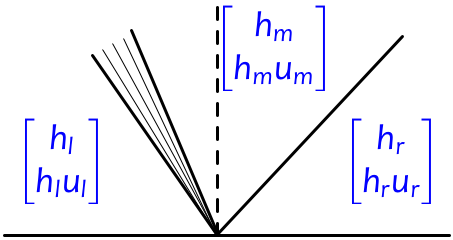
\includegraphics{./figures/shallow_water_riemann.png}
\caption{Structure of Riemann solution}
\end{figure}

In the figure we have one wave going in each direction, but since the
wave speeds depend on \(q\) and can have either sign, it is possible to
have both waves going left, or both going right. In these cases, the
flow is said to be \emph{supercritical}.

To solve the Riemann problem, we must find \(q_m\). To do so we must
find a state that can be connected to \(q_\ell\) by a 1-shock or
1-rarefaction and to \(q_r\) by a 2-shock or 2-rarefaction. We must also
ensure that the resulting waves satisfy the entropy condition.

\hypertarget{shock-waves}{%
\section{Shock waves}\label{shock-waves}}

Let us now consider a shock wave connecting a known state
\(q_*=(h_*, h_* u_*)\) to an unknown state \(q=(h,hu)\). In the context
of the Riemann problem, \(q_*\) will be the known left or right state
and \(q\) will be the unknown middle state. The Rankine--Hugoniot jump
conditions \(s(q_* - q) = f(q_*) - f(q)\) for a shock wave moving at
speed \(s\) read as

\begin{align}
s (h_* - h) & = h_* u_* - h u, \\
s (h_* u_* - h u) & = h_* u_*^2 - h u^2 + \frac{g}{2}(h_*^2 - h^2).
\end{align}

It is convenient to define \(\alpha = h - h_*\). Then we can combine the
two equations above to show that the momenta are related by
\begin{align} \label{SW:hugoniot-locus}
    h u & = h_* u_* + \alpha \left[u_* \pm \sqrt{gh_* \left(1+\frac{\alpha}{h_*}\right)\left(1+\frac{\alpha}{2h_*}\right)}\right]
\end{align} for a shock moving with speed
\begin{align} \label{SW:shock-speed}
    s & = \frac{h_* u_* - h u}{h_* - h} = u_* \mp \sqrt{gh_* \left(1+\frac{\alpha}{h_*}\right)\left(1+\frac{\alpha}{2h_*}\right)} = u_* \mp \sqrt{gh \frac{h_* + h}{2h_*} }.
\end{align}

Choosing the plus sign in (\ref{SW:hugoniot-locus}) (which yields the
minus sign in (\ref{SW:shock-speed})) gives a 1-shock. Choosing the
minus sign in (\ref{SW:hugoniot-locus}) (which yields the plus sign in
(\ref{SW:shock-speed})) gives a 2-shock. Notice from the last expression
in (\ref{SW:shock-speed}) that as \(h \to h^*\) the shock speed
approaches the corresponding characteristic speed
(\ref{SW:char-speeds}), while the ratio of the jumps in momentum and
depth approaches that suggested by the eigenvectors
(\ref{SW:fjac-evecs}).

We can now consider the set of all possible states \((h, h u)\)
satisfying (\ref{SW:hugoniot-locus}). This curve in the \(h - hu\) plane
is known as the Hugoniot locus; there is a family of Hugoniot loci for
1-shocks and another for 2-shocks. Below we plot some members of the
1-loci of curves. \emph{In the interactive notebook you can select the
2-loci instead.}

    \begin{Verbatim}[fontsize=\small,commandchars=\\\{\}]
{\color{incolor}In [{\color{incolor}4}]:} \PY{n}{interact}\PY{p}{(}\PY{n}{shallow\PYZus{}water}\PY{o}{.}\PY{n}{plot\PYZus{}hugoniot\PYZus{}loci}\PY{p}{,} \PY{n}{y\PYZus{}axis}\PY{o}{=}\PY{n}{widgets}\PY{o}{.}\PY{n}{fixed}\PY{p}{(}\PY{l+s+s1}{\PYZsq{}}\PY{l+s+s1}{hu}\PY{l+s+s1}{\PYZsq{}}\PY{p}{)}\PY{p}{,}
                 \PY{n}{plot\PYZus{}1}\PY{o}{=}\PY{n}{widgets}\PY{o}{.}\PY{n}{Checkbox}\PY{p}{(}\PY{n}{description}\PY{o}{=}\PY{l+s+s1}{\PYZsq{}}\PY{l+s+s1}{Plot 1\PYZhy{}loci}\PY{l+s+s1}{\PYZsq{}}\PY{p}{,}\PY{n}{value}\PY{o}{=}\PY{k+kc}{True}\PY{p}{)}\PY{p}{,}
                 \PY{n}{plot\PYZus{}2}\PY{o}{=}\PY{n}{widgets}\PY{o}{.}\PY{n}{Checkbox}\PY{p}{(}\PY{n}{description}\PY{o}{=}\PY{l+s+s1}{\PYZsq{}}\PY{l+s+s1}{Plot 2\PYZhy{}loci}\PY{l+s+s1}{\PYZsq{}}\PY{p}{,}\PY{n}{value}\PY{o}{=}\PY{k+kc}{False}\PY{p}{)}\PY{p}{)}\PY{p}{;}
\end{Verbatim}

    \begin{center}
    \adjustimage{max size={0.9\linewidth}{0.9\paperheight}}{combined_files/combined_210_0.pdf}
    \end{center}
    { \hspace*{\fill} \\}
    
The plot above shows the Hugoniot loci in the \(h\)-\(hu\) plane, the
natural phase plane in terms of the two conserved quantities. Of course,
they all approach the origin as \(h \rightarrow 0\). Alternatively, we
can plot these same curves in the \(h\)-\(u\) plane:

    \begin{Verbatim}[fontsize=\small,commandchars=\\\{\}]
{\color{incolor}In [{\color{incolor}5}]:} \PY{n}{interact}\PY{p}{(}\PY{n}{shallow\PYZus{}water}\PY{o}{.}\PY{n}{plot\PYZus{}hugoniot\PYZus{}loci}\PY{p}{,} \PY{n}{y\PYZus{}axis}\PY{o}{=}\PY{n}{widgets}\PY{o}{.}\PY{n}{fixed}\PY{p}{(}\PY{l+s+s1}{\PYZsq{}}\PY{l+s+s1}{u}\PY{l+s+s1}{\PYZsq{}}\PY{p}{)}\PY{p}{,}
                 \PY{n}{plot\PYZus{}1}\PY{o}{=}\PY{n}{widgets}\PY{o}{.}\PY{n}{Checkbox}\PY{p}{(}\PY{n}{description}\PY{o}{=}\PY{l+s+s1}{\PYZsq{}}\PY{l+s+s1}{Plot 1\PYZhy{}loci}\PY{l+s+s1}{\PYZsq{}}\PY{p}{,}\PY{n}{value}\PY{o}{=}\PY{k+kc}{True}\PY{p}{)}\PY{p}{,}
                 \PY{n}{plot\PYZus{}2}\PY{o}{=}\PY{n}{widgets}\PY{o}{.}\PY{n}{Checkbox}\PY{p}{(}\PY{n}{description}\PY{o}{=}\PY{l+s+s1}{\PYZsq{}}\PY{l+s+s1}{Plot 2\PYZhy{}loci}\PY{l+s+s1}{\PYZsq{}}\PY{p}{,}\PY{n}{value}\PY{o}{=}\PY{k+kc}{False}\PY{p}{)}\PY{p}{)}\PY{p}{;}
\end{Verbatim}

    \begin{center}
    \adjustimage{max size={0.9\linewidth}{0.9\paperheight}}{combined_files/combined_212_0.pdf}
    \end{center}
    { \hspace*{\fill} \\}
    
Note that in this plane the curves in each family are simply vertical
translates of one another, and all curves asymptote to \(\pm \infty\) as
\(h \rightarrow 0\). This means that it is impossible to have a shock
with an adjacent dry (\(h=0\)) state.

\hypertarget{all-shock-riemann-solutions}{%
\subsection{All-shock Riemann
solutions}\label{all-shock-riemann-solutions}}

If we knew a priori that both waves in the Riemann solution were shock
waves, we could find \(q_m\) by finding the intersection of the
1-Hugoniot locus passing through \(q_\ell\) with the 2-Hugoniot locus
passing through \(q_r\). The Riemann solution would then consist simply
of two discontinuities propagating at the speeds given by
(\ref{SW:shock-speed}).

Here is an example for which this is the correct solution: The initial
depth is the same everywhere, \(h_\ell=h_r\), but the velocity
\(u_\ell>0\) while \(u_r<0\) so the flow is toward \(x=0\) from both
sides. Note that in this plot the dark and light blue stripes show a
passive tracer advected with the flow, which is shown only to help
visualize the fluid velocity in these plots.

    \begin{Verbatim}[fontsize=\small,commandchars=\\\{\}]
{\color{incolor}In [{\color{incolor}6}]:} \PY{n}{shallow\PYZus{}water}\PY{o}{.}\PY{n}{plot\PYZus{}riemann\PYZus{}SW}\PY{p}{(}\PY{n}{h\PYZus{}l}\PY{o}{=}\PY{l+m+mi}{2}\PY{p}{,} \PY{n}{h\PYZus{}r}\PY{o}{=}\PY{l+m+mi}{2}\PY{p}{,} \PY{n}{u\PYZus{}l}\PY{o}{=}\PY{l+m+mi}{1}\PY{p}{,} \PY{n}{u\PYZus{}r}\PY{o}{=}\PY{o}{\PYZhy{}}\PY{l+m+mi}{1}\PY{p}{)}
\end{Verbatim}

    \begin{center}
    \adjustimage{max size={0.9\linewidth}{0.9\paperheight}}{combined_files/combined_215_0.pdf}
    \end{center}
    { \hspace*{\fill} \\}
    
    \begin{center}
    \adjustimage{max size={0.9\linewidth}{0.9\paperheight}}{combined_files/combined_215_1.pdf}
    \end{center}
    { \hspace*{\fill} \\}
    
    \begin{center}
    \adjustimage{max size={0.9\linewidth}{0.9\paperheight}}{combined_files/combined_215_2.pdf}
    \end{center}
    { \hspace*{\fill} \\}
    
\emph{In the interactive notebook you can check the boxes to plot the
characteristic families, and notice that the} 1-\emph{characteristics
impinge on the} 1-\emph{shock; the} 2-\emph{characteristics impinge on
the} 2-\emph{shock. Thus these shocks satisfy the entropy condition. You
can also check a box to show the particle paths, which show how the
water is decelerated to} 0 \emph{speed as it goes through each shock.}

\hypertarget{dam-break-problem-all-shock-solution}{%
\subsubsection{Dam-break problem: all-shock
solution}\label{dam-break-problem-all-shock-solution}}

Here's another example, which you might think of as modeling a dam that
suddenly breaks. The water is initially at rest on both sides, but much
deeper on the left. We can again construct a 2-shock Riemann solution,
but \emph{this is not physically correct in this case!}

    \begin{Verbatim}[fontsize=\small,commandchars=\\\{\}]
{\color{incolor}In [{\color{incolor}7}]:} \PY{n}{shallow\PYZus{}water}\PY{o}{.}\PY{n}{plot\PYZus{}riemann\PYZus{}SW}\PY{p}{(}\PY{n}{h\PYZus{}l}\PY{o}{=}\PY{l+m+mi}{4}\PY{p}{,} \PY{n}{h\PYZus{}r}\PY{o}{=}\PY{l+m+mi}{1}\PY{p}{,} \PY{n}{u\PYZus{}l}\PY{o}{=}\PY{l+m+mi}{0}\PY{p}{,} \PY{n}{u\PYZus{}r}\PY{o}{=}\PY{l+m+mi}{0}\PY{p}{,} \PY{n}{plot1}\PY{o}{=}\PY{k+kc}{True}\PY{p}{,}
                                      \PY{n}{force\PYZus{}waves}\PY{o}{=}\PY{l+s+s1}{\PYZsq{}}\PY{l+s+s1}{shock}\PY{l+s+s1}{\PYZsq{}}\PY{p}{,} \PY{n}{particle\PYZus{}paths}\PY{o}{=}\PY{k+kc}{False}\PY{p}{)}\PY{p}{;}
\end{Verbatim}

    \begin{center}
    \adjustimage{max size={0.9\linewidth}{0.9\paperheight}}{combined_files/combined_218_0.pdf}
    \end{center}
    { \hspace*{\fill} \\}
    
    \begin{center}
    \adjustimage{max size={0.9\linewidth}{0.9\paperheight}}{combined_files/combined_218_1.pdf}
    \end{center}
    { \hspace*{\fill} \\}
    
    \begin{center}
    \adjustimage{max size={0.9\linewidth}{0.9\paperheight}}{combined_files/combined_218_2.pdf}
    \end{center}
    { \hspace*{\fill} \\}
    
Notice that the 1-characteristics (which are plotted as thin lines)
don't impinge on the 1-shock; instead, characteristics are diverging
away from it. This shock does not satisfy the entropy condition and
should be replaced with a rarefaction. The corresponding part of the
Hugoniot locus is plotted with a dashed line to remind us that it is
unphysical.

\emph{Now check the box to plot the} 2-\emph{characteristics.} Notice
that these \emph{do} impinge on the 2-shock; this is an
entropy-satisfying shock, and the Hugoniot locus is plotted as a solid
line.

\hypertarget{the-entropy-condition}{%
\subsection{The entropy condition}\label{the-entropy-condition}}

For the 2-shock Riemann solution to be physically correct, each of the
waves must satisfy the Lax entropy condition, with the characteristic
speed to the left of the wave greater than that to the right. Notice
that the shock speed (\ref{SW:shock-speed}) can be written as

\begin{align}
    s & = u_* \pm \sqrt{gh \frac{h_* + h}{2h_*} }.
\end{align}\\
Thus the 1-shock entropy condition reads as

\begin{align*}
u_\ell - \sqrt{gh_\ell} > u_\ell - \sqrt{gh_\ell \frac{h_\ell+h_m}{2h_\ell}} = u_m - \sqrt{gh_m \frac{h_m+h_\ell}{2h_m}} > u_m - \sqrt{gh_m}.
\end{align*}\\
The second expression for the shock speed is obtained by noticing that
the shock speed is invariant under transposition of the left and right
states. The first and second inequalities both simplify to

\begin{align} \label{SW:1-entropy}
    h_m > h_\ell.
\end{align}\\
Similarly, it can be shown that the entropy condition for a 2-shock
connecting \(q_m\) and \(q_r\) is satisfied if and only if

\begin{align} \label{SW:2-entropy}
    h_m > h_r.
\end{align}\\
If (\ref{SW:1-entropy}) or (\ref{SW:2-entropy}) is violated, then the
corresponding wave must be a rarefaction rather than a shock.

Go back and look at the phase plane plots above. You'll notice that the
1-Hugoniot locus passing through \(q_\ell\) is plotted with a solid line
for \(h>h_\ell\) and with a dashed line for \(h<h_\ell\) (and the same
is done for the 2-Hugoniot locus passing through \(q_r\)). This is to
remind us that states connected to \(q_\ell\) by the dashed part are
unphysical.

\hypertarget{rarefaction-waves}{%
\section{Rarefaction waves}\label{rarefaction-waves}}

\hypertarget{integral-curves}{%
\subsection{Integral curves}\label{integral-curves}}

In the LWR traffic flow model, we saw that a rarefaction wave consisted
of a smoothly varying density. For the shallow water system, both the
depth \(h\) and the momentum \(hu\) will vary smoothly through a
rarefaction wave. A given rarefaction wave is associated with just one
characteristic family, and the variation within the wave is at all
points proportional to the corresponding eigenvector \(r_p\). In other
words, all values \(\tilde{q}=(h,hu)\) in the rarefaction lie on a curve
defined by

\begin{align} \label{SW:gen_ode}
    \tilde{q}'(\xi) & = r_p(\tilde{q}(\xi)).
\end{align}

Here \(\tilde{q}(\xi)\) is a parameterization of the solution. For the
shallow water system, (\ref{SW:gen_ode}) reads as

\begin{align}
    h'(\xi)    = q_1'(\xi) & = 1 \label{SW:dh}, \\
    (hu)'(\xi) = q_2'(\xi) & = u \pm \sqrt{gh} = \tilde{q}_2/\tilde{q}_1 - \sqrt{g\tilde{q}_1}, \label{SW:dhu}
\end{align}\\
where we take the minus sign for 1-waves and the plus sign for 2-waves.
We can think of (\ref{SW:dh})-(\ref{SW:dhu}) as an initial value ODE;
fixing the value of \(\tilde{q}\) at one point in the rarefaction wave
determines the whole solution of (\ref{SW:dh})-(\ref{SW:dhu}). We refer
to each of these solutions as an \emph{integral curve}.

For the shallow water system, these equations can be integrated exactly.
If we fix one point \((h_*, h_*u_*)\) on the curve, the whole integral
curve is defined by

\begin{align}
    hu & = hu_* \pm 2h(\sqrt{gh_*} - \sqrt{gh}),
\end{align}\\
where now the plus sign is for 1-waves and the minus sign for 2-waves.
This can be rewritten as

\begin{align} \label{SW:riemann-invariant}
u \pm 2 \sqrt{gh} = u_* \pm 2 \sqrt{gh_*}.
\end{align}\\
From (\ref{SW:riemann-invariant}) we see that the value
\(u + 2 \sqrt{gh}\) is constant along any 1-integral curve, while the
value \(u-2\sqrt{gh}\) is constant along any 2-integral curve. We refer
to these quantities as \emph{Riemann invariants} for the shallow water
system:

\begin{align}
w_1(q) & = u + 2 \sqrt{gh}, \\
w_2(q) & = u - 2 \sqrt{gh}.
\end{align}\\
In other words, the trajectories plotted above are just the level curves
of \(w_1\) and \(w_2\). This allows us to easily plot the integral
curves as a contour plot of \(w_1\) or \(w_2\). \emph{In the notebook
you can select which family of curves to display.}

    \begin{Verbatim}[fontsize=\small,commandchars=\\\{\}]
{\color{incolor}In [{\color{incolor}8}]:} \PY{n}{interact}\PY{p}{(}\PY{n}{shallow\PYZus{}demos}\PY{o}{.}\PY{n}{plot\PYZus{}int\PYZus{}curves}\PY{p}{,} \PY{n}{y\PYZus{}axis}\PY{o}{=}\PY{n}{widgets}\PY{o}{.}\PY{n}{fixed}\PY{p}{(}\PY{l+s+s1}{\PYZsq{}}\PY{l+s+s1}{hu}\PY{l+s+s1}{\PYZsq{}}\PY{p}{)}\PY{p}{,}
                 \PY{n}{plot\PYZus{}1}\PY{o}{=}\PY{n}{widgets}\PY{o}{.}\PY{n}{Checkbox}\PY{p}{(}\PY{n}{description}\PY{o}{=}\PY{l+s+s1}{\PYZsq{}}\PY{l+s+s1}{1\PYZhy{}wave curves}\PY{l+s+s1}{\PYZsq{}}\PY{p}{,}
                                         \PY{n}{value}\PY{o}{=}\PY{k+kc}{True}\PY{p}{)}\PY{p}{,}
                 \PY{n}{plot\PYZus{}2}\PY{o}{=}\PY{n}{widgets}\PY{o}{.}\PY{n}{Checkbox}\PY{p}{(}\PY{n}{description}\PY{o}{=}\PY{l+s+s1}{\PYZsq{}}\PY{l+s+s1}{2\PYZhy{}wave curves}\PY{l+s+s1}{\PYZsq{}}\PY{p}{,}
                                         \PY{n}{value}\PY{o}{=}\PY{k+kc}{False}\PY{p}{)}\PY{p}{)}\PY{p}{;}
\end{Verbatim}

    \begin{center}
    \adjustimage{max size={0.9\linewidth}{0.9\paperheight}}{combined_files/combined_223_0.pdf}
    \end{center}
    { \hspace*{\fill} \\}
    
We can also plot the integral curves in the \(h\)--\(u\) plane:

    \begin{Verbatim}[fontsize=\small,commandchars=\\\{\}]
{\color{incolor}In [{\color{incolor}9}]:} \PY{n}{interact}\PY{p}{(}\PY{n}{shallow\PYZus{}demos}\PY{o}{.}\PY{n}{plot\PYZus{}int\PYZus{}curves}\PY{p}{,} \PY{n}{y\PYZus{}axis}\PY{o}{=}\PY{n}{widgets}\PY{o}{.}\PY{n}{fixed}\PY{p}{(}\PY{l+s+s1}{\PYZsq{}}\PY{l+s+s1}{u}\PY{l+s+s1}{\PYZsq{}}\PY{p}{)}\PY{p}{,}
                 \PY{n}{plot\PYZus{}1}\PY{o}{=}\PY{n}{widgets}\PY{o}{.}\PY{n}{Checkbox}\PY{p}{(}\PY{n}{description}\PY{o}{=}\PY{l+s+s1}{\PYZsq{}}\PY{l+s+s1}{1\PYZhy{}wave curves}\PY{l+s+s1}{\PYZsq{}}\PY{p}{,}
                                         \PY{n}{value}\PY{o}{=}\PY{k+kc}{True}\PY{p}{)}\PY{p}{,}
                 \PY{n}{plot\PYZus{}2}\PY{o}{=}\PY{n}{widgets}\PY{o}{.}\PY{n}{Checkbox}\PY{p}{(}\PY{n}{description}\PY{o}{=}\PY{l+s+s1}{\PYZsq{}}\PY{l+s+s1}{2\PYZhy{}wave curves}\PY{l+s+s1}{\PYZsq{}}\PY{p}{,}
                                         \PY{n}{value}\PY{o}{=}\PY{k+kc}{False}\PY{p}{)}\PY{p}{)}\PY{p}{;}
\end{Verbatim}

    \begin{center}
    \adjustimage{max size={0.9\linewidth}{0.9\paperheight}}{combined_files/combined_225_0.pdf}
    \end{center}
    { \hspace*{\fill} \\}
    
Note that in this plane the integral curves of each family are simply
vertical translates of one another due to the form of the functions
\(w_1\) and \(w_2\). Unlike the Hugoniot loci, the integral curves do
not asymptote to \(\pm\infty\) as \(h \rightarrow 0\) and instead each
approaches a finite value.

\hypertarget{comparison-of-integral-curves-and-hugoniot-loci}{%
\subsection{Comparison of integral curves and Hugoniot
loci}\label{comparison-of-integral-curves-and-hugoniot-loci}}

You may have noticed that the integral curves look very similar to the
Hugoniot loci, especially when plotted in the \(h-hu\) plane. Below we
emphasize the differences by plotting the curve from each of these
families that passes through a specified point. The difference is less
noticeable in the \(h-hu\) plane since all of the curves approach the
origin.

\emph{In the notebook you can select which family to display.}

    \begin{Verbatim}[fontsize=\small,commandchars=\\\{\}]
{\color{incolor}In [{\color{incolor}10}]:} \PY{n}{interact}\PY{p}{(}\PY{n}{shallow\PYZus{}demos}\PY{o}{.}\PY{n}{compare\PYZus{}curves}\PY{p}{,}
                  \PY{n}{wave\PYZus{}family}\PY{o}{=}\PY{n}{RadioButtons}\PY{p}{(}\PY{n}{options}\PY{o}{=}\PY{p}{[}\PY{l+m+mi}{1}\PY{p}{,}\PY{l+m+mi}{2}\PY{p}{]}\PY{p}{,}
                                           \PY{n}{description}\PY{o}{=}\PY{l+s+s1}{\PYZsq{}}\PY{l+s+s1}{Wave family:}\PY{l+s+s1}{\PYZsq{}}\PY{p}{)}\PY{p}{,}
                  \PY{n}{y\PYZus{}axis}\PY{o}{=}\PY{n}{RadioButtons}\PY{p}{(}\PY{n}{options}\PY{o}{=}\PY{p}{[}\PY{l+s+s1}{\PYZsq{}}\PY{l+s+s1}{u}\PY{l+s+s1}{\PYZsq{}}\PY{p}{,}\PY{l+s+s1}{\PYZsq{}}\PY{l+s+s1}{hu}\PY{l+s+s1}{\PYZsq{}}\PY{p}{]}\PY{p}{,}
                                      \PY{n}{description}\PY{o}{=}\PY{l+s+s1}{\PYZsq{}}\PY{l+s+s1}{Vertical axis:}\PY{l+s+s1}{\PYZsq{}}\PY{p}{)}\PY{p}{,}
                  \PY{n}{h0}\PY{o}{=}\PY{n}{FloatSlider}\PY{p}{(}\PY{n+nb}{min}\PY{o}{=}\PY{l+m+mf}{1.e\PYZhy{}1}\PY{p}{,}\PY{n+nb}{max}\PY{o}{=}\PY{l+m+mf}{3.}\PY{p}{,}\PY{n}{value}\PY{o}{=}\PY{l+m+mf}{1.}\PY{p}{,}
                                 \PY{n}{description}\PY{o}{=}\PY{l+s+s1}{\PYZsq{}}\PY{l+s+s1}{\PYZdl{}h\PYZus{}*\PYZdl{}}\PY{l+s+s1}{\PYZsq{}}\PY{p}{)}\PY{p}{,}
                  \PY{n}{u0}\PY{o}{=}\PY{n}{FloatSlider}\PY{p}{(}\PY{n+nb}{min}\PY{o}{=}\PY{o}{\PYZhy{}}\PY{l+m+mi}{3}\PY{p}{,}\PY{n+nb}{max}\PY{o}{=}\PY{l+m+mi}{3}\PY{p}{,}\PY{n}{description}\PY{o}{=}\PY{l+s+s1}{\PYZsq{}}\PY{l+s+s1}{\PYZdl{}u\PYZus{}*\PYZdl{}}\PY{l+s+s1}{\PYZsq{}}\PY{p}{)}\PY{p}{)}\PY{p}{;}
\end{Verbatim}

    \begin{center}
    \adjustimage{max size={0.9\linewidth}{0.9\paperheight}}{combined_files/combined_228_0.pdf}
    \end{center}
    { \hspace*{\fill} \\}
    
Near the point of intersection, the curves are very close; indeed, they
must be tangent at this point since their direction is parallel to the
corresponding eigenvector there (and in fact they also have the same
curvature). Far from this point they diverge; for small depths they must
diverge greatly, since the Hugoniot locus never reaches \(h=0\) at any
finite velocity.

\hypertarget{the-structure-of-centered-rarefaction-waves}{%
\subsection{The structure of centered rarefaction
waves}\label{the-structure-of-centered-rarefaction-waves}}

Rarefactions appearing in the Riemann solution are also similarity
solutions; that is, they are constant along any ray \(\xi=x/t\). For a
\(p\)-rarefaction connecting states \(q_\ell\) and \(q_r\), the
rarefaction thus has the form

\begin{align}
    q(x,t) & = \begin{cases} q_\ell & \text{if } x/t \le \lambda_p(q_\ell), \\
                            \tilde{q}(x/t) & \text{if } \lambda_p(q_\ell) \le \lambda_p(q_r), \\
                            q_r & \text{if } x/t \ge \lambda_p(q_r). \end{cases}
\end{align}

It remains to be determined how \(\tilde{q}\) varies as a function of
\(x/t\). This can be determined by noting that each solution value
\(\tilde{q}\) propagates at the characteristic speed
\(\lambda_p(\tilde{q})\). Letting \(\xi=x/t\), this gives us the
condition

\begin{align} \label{SW:char-sim}
    \lambda_p(\tilde{q}(\xi)) = \xi.
\end{align}

By combining (\ref{SW:char-sim}) with the Riemann invariant condition,
we can find \(\tilde{h}\) and \(\tilde{u}\) within the rarefaction. For
concreteness, let us consider a 1-rarefaction connecting \(q_\ell\) and
\(q_m\). Then (\ref{SW:char-sim}) reads
\(\tilde{u} - \sqrt{g\tilde{h}} = \xi\), which simplifies to

\begin{align} \label{SW:char-sim1}
\tilde{h} = \frac{(\tilde{u}-\xi)^2}{g}.
\end{align}\\
Meanwhile, the fact that \(w_1(\tilde{q})\) is constant means that

\begin{align} \label{SW:w1-const}
    \tilde{u} + 2 \sqrt{g\tilde{h}} = u_\ell + 2 \sqrt{gh_\ell}.
\end{align}\\
Combining (\ref{SW:char-sim1}) with (\ref{SW:w1-const}), we find

\begin{align} \label{SW:1-raref-struct-h}
    \tilde{h} & = \frac{(u_\ell + 2\sqrt{gh_\ell} - \xi)^2}{9g} = \frac{(w_1(q_\ell) - \xi)^2}{9g}, \\
    \tilde{u} & = \frac{1}{3}w_1(q_\ell) + \frac{2}{3}\xi. \label{SW:1-raref-struct-u}
\end{align}\\
We see that \(h\) varies quadratically through the rarefaction, while
\(u\) varies linearly.

\hypertarget{connecting-states}{%
\subsection{Connecting states}\label{connecting-states}}

Suppose we know that the middle state \(q_m\) is connected to the left
and right states by rarefactions. Then we can find \(q_m\) by finding
the intersection of the corresponding integral curves. Here is an
example for which this is the physically correct solution:

\begin{align}
    q_\ell & = \begin{bmatrix} 1 \\ -1 \end{bmatrix}, &
    q_r & = \begin{bmatrix} 1 \\ 1 \end{bmatrix}.
\end{align}

In this case the water is flowing \emph{away} from \(x=0\) on both
sides.

    \begin{Verbatim}[fontsize=\small,commandchars=\\\{\}]
{\color{incolor}In [{\color{incolor}11}]:} \PY{n}{shallow\PYZus{}water}\PY{o}{.}\PY{n}{plot\PYZus{}riemann\PYZus{}SW}\PY{p}{(}\PY{n}{h\PYZus{}l}\PY{o}{=}\PY{l+m+mi}{1}\PY{p}{,} \PY{n}{h\PYZus{}r}\PY{o}{=}\PY{l+m+mi}{1}\PY{p}{,} \PY{n}{u\PYZus{}l}\PY{o}{=}\PY{o}{\PYZhy{}}\PY{l+m+mf}{1.}\PY{p}{,} \PY{n}{u\PYZus{}r}\PY{o}{=}\PY{l+m+mf}{1.}\PY{p}{)}
\end{Verbatim}

    \begin{center}
    \adjustimage{max size={0.9\linewidth}{0.9\paperheight}}{combined_files/combined_232_0.pdf}
    \end{center}
    { \hspace*{\fill} \\}
    
    \begin{center}
    \adjustimage{max size={0.9\linewidth}{0.9\paperheight}}{combined_files/combined_232_1.pdf}
    \end{center}
    { \hspace*{\fill} \\}
    
    \begin{center}
    \adjustimage{max size={0.9\linewidth}{0.9\paperheight}}{combined_files/combined_232_2.pdf}
    \end{center}
    { \hspace*{\fill} \\}
    
Notice that the segment of each integral curve that connects to states
with a smaller depth is plotted as a solid line, while the segment
connecting to states with greater depth is plotted with a dashed line.
This again is to remind us that states connected by a rarefaction
through the solid part are physical (entropy-satisfying), while states
connected by the dashed part would be unphysical (entropy-violating).

\emph{Try changing the velocities to \((1.9, -1.9)\), and notice that
the Riemann solution has a state with almost zero depth in the middle.
What happens if you use even larger outflow velocities? We'll discuss
this later, in the section on dry states.}

\hypertarget{dam-break-problem-all-rarefaction-solution}{%
\subsection{Dam-break problem: all-rarefaction
solution}\label{dam-break-problem-all-rarefaction-solution}}

Next let us revisit the problem from
Section \ref{dam-break-problem-all-shock-solution} where we found that
the all-shock solution was incorrect. This time we'll try to find an
all-rarefaction solution.

    \begin{Verbatim}[fontsize=\small,commandchars=\\\{\}]
{\color{incolor}In [{\color{incolor}12}]:} \PY{n}{shallow\PYZus{}water}\PY{o}{.}\PY{n}{plot\PYZus{}riemann\PYZus{}SW}\PY{p}{(}\PY{n}{h\PYZus{}l}\PY{o}{=}\PY{l+m+mi}{4}\PY{p}{,} \PY{n}{h\PYZus{}r}\PY{o}{=}\PY{l+m+mi}{1}\PY{p}{,} \PY{n}{u\PYZus{}l}\PY{o}{=}\PY{l+m+mi}{0}\PY{p}{,} \PY{n}{u\PYZus{}r}\PY{o}{=}\PY{l+m+mi}{0}\PY{p}{,} \PY{n}{plot2}\PY{o}{=}\PY{k+kc}{True}\PY{p}{,}
                                       \PY{n}{force\PYZus{}waves}\PY{o}{=}\PY{l+s+s1}{\PYZsq{}}\PY{l+s+s1}{raref}\PY{l+s+s1}{\PYZsq{}}\PY{p}{,} \PY{n}{particle\PYZus{}paths}\PY{o}{=}\PY{k+kc}{False}\PY{p}{)}
\end{Verbatim}

    \begin{center}
    \adjustimage{max size={0.9\linewidth}{0.9\paperheight}}{combined_files/combined_236_0.pdf}
    \end{center}
    { \hspace*{\fill} \\}
    
    \begin{center}
    \adjustimage{max size={0.9\linewidth}{0.9\paperheight}}{combined_files/combined_236_1.pdf}
    \end{center}
    { \hspace*{\fill} \\}
    
    \begin{center}
    \adjustimage{max size={0.9\linewidth}{0.9\paperheight}}{combined_files/combined_236_2.pdf}
    \end{center}
    { \hspace*{\fill} \\}
    
Notice that the 2-characteristics (plotted as thin lines) impinge on the
2-rarefaction; in fact they intersect at the left edge of the
rarefaction. This means that the solution we constructed is
triple-valued and nonsensical as a solution to this one-dimensional
conservation law, and so this portion of the solution is omitted in the
plots of depth and momentum. In this case a rarefaction wave is not
physical and should be replaced with a shock; the corresponding part of
the integral curve is hence shown as a dashed line.

\hypertarget{the-riemann-solution}{%
\section{The Riemann solution}\label{the-riemann-solution}}

To determine \(q_m\), we need to know whether each of the two waves is a
shock or rarefaction, so that we can use the appopriate Hugoniot locus
or integral curve. But to determine the nature of each wave, we need to
check (\ref{SW:1-entropy}) or (\ref{SW:2-entropy}), which requires
knowledge of \(h_m\). To deal with this we define a piecewise function
\(\phi_\ell(h)\) that gives

\begin{itemize}
\tightlist
\item
  for \(h>h_\ell\), the momentum connected to \(q_\ell\) by a 1-shock;
\item
  for \(h<h_\ell\), the momentum connected to \(q_\ell\) by a 1-integral
  curve.
\end{itemize}

Thus \(\phi\) is partly a 1-Hugoniot locus and partly a 1-integral
curve; it gives the value of each precisely in the regime where they are
physically correct. We can similarly define a function \(\phi_r(h)\)
related to the 2-Hugoniot locus and 2-integral curve. The middle state
depth \(h_m\) is the value for which \(\phi_\ell(h) = \phi_r(h)\). This
value can be found computationally via a rootfinding algorithm.

\hypertarget{dam-break-problem-correct-solution}{%
\subsection{Dam-break problem: correct
solution}\label{dam-break-problem-correct-solution}}

Below we plot (at last) the correct solution to the dam-break problem,
involving a 1-rarefaction and a 2-shock. Plot the characteristics and
notice how each family behaves correctly with respect to the
corresponding wave in the Riemann solution.

    \begin{Verbatim}[fontsize=\small,commandchars=\\\{\}]
{\color{incolor}In [{\color{incolor}13}]:} \PY{n}{shallow\PYZus{}water}\PY{o}{.}\PY{n}{plot\PYZus{}riemann\PYZus{}SW}\PY{p}{(}\PY{n}{h\PYZus{}l}\PY{o}{=}\PY{l+m+mi}{4}\PY{p}{,} \PY{n}{h\PYZus{}r}\PY{o}{=}\PY{l+m+mi}{1}\PY{p}{,} \PY{n}{u\PYZus{}l}\PY{o}{=}\PY{l+m+mi}{0}\PY{p}{,} \PY{n}{u\PYZus{}r}\PY{o}{=}\PY{l+m+mi}{0}\PY{p}{)}
\end{Verbatim}

    \begin{center}
    \adjustimage{max size={0.9\linewidth}{0.9\paperheight}}{combined_files/combined_240_0.pdf}
    \end{center}
    { \hspace*{\fill} \\}
    
    \begin{center}
    \adjustimage{max size={0.9\linewidth}{0.9\paperheight}}{combined_files/combined_240_1.pdf}
    \end{center}
    { \hspace*{\fill} \\}
    
    \begin{center}
    \adjustimage{max size={0.9\linewidth}{0.9\paperheight}}{combined_files/combined_240_2.pdf}
    \end{center}
    { \hspace*{\fill} \\}
    
\emph{In the interactive notebook you can confirm that}
1-\emph{charactersitics spread out across the rarefaction fan while}
2-\emph{characteristics converge on the shock. View the particle paths
and note that between the two waves the fluid velocity is constant, with
the fluid accelerating across both the rarefaction and shock to the same
intermediate value \(u_m\).}

\hypertarget{dry-states}{%
\section{Dry states}\label{dry-states}}

The approach just described will yield the correct Riemann solution
(provided that the rootfinding algorithm converges) in most situations.
However, it will fail if the solution involves dry (\(h=0\)) states.

\hypertarget{dry-middle-state}{%
\subsection{Dry middle state}\label{dry-middle-state}}

Sometimes it seems that there is no way to connect a given pair of left
and right states via entropy-satisfying shocks or rarefactions. In the
cell below we plot only the physically relevant parts of the integral
curves and Hugoniot loci passing through the left and right states. Both
the \(h-u\) and \(h-hu\) planes are shown. \emph{With the interactive
widget you can try to adjust those states to find a combination for
which none of the curves intersect.}

    \begin{Verbatim}[fontsize=\small,commandchars=\\\{\}]
{\color{incolor}In [{\color{incolor}14}]:} \PY{n}{interact}\PY{p}{(}\PY{n}{shallow\PYZus{}demos}\PY{o}{.}\PY{n}{connect\PYZus{}states}\PY{p}{,}
                  \PY{n}{h\PYZus{}l}\PY{o}{=}\PY{n}{widgets}\PY{o}{.}\PY{n}{FloatSlider}\PY{p}{(}\PY{n+nb}{min}\PY{o}{=}\PY{l+m+mf}{0.001}\PY{p}{,}\PY{n+nb}{max}\PY{o}{=}\PY{l+m+mi}{2}\PY{p}{,}\PY{n}{value}\PY{o}{=}\PY{l+m+mi}{1}\PY{p}{)}\PY{p}{,}
                  \PY{n}{u\PYZus{}l}\PY{o}{=}\PY{n}{widgets}\PY{o}{.}\PY{n}{FloatSlider}\PY{p}{(}\PY{n+nb}{min}\PY{o}{=}\PY{o}{\PYZhy{}}\PY{l+m+mi}{5}\PY{p}{,}\PY{n+nb}{max}\PY{o}{=}\PY{l+m+mi}{5}\PY{p}{,}\PY{n}{value}\PY{o}{=}\PY{o}{\PYZhy{}}\PY{l+m+mi}{1}\PY{p}{)}\PY{p}{,}
                  \PY{n}{h\PYZus{}r}\PY{o}{=}\PY{n}{widgets}\PY{o}{.}\PY{n}{FloatSlider}\PY{p}{(}\PY{n+nb}{min}\PY{o}{=}\PY{l+m+mf}{0.001}\PY{p}{,}\PY{n+nb}{max}\PY{o}{=}\PY{l+m+mi}{2}\PY{p}{,}\PY{n}{value}\PY{o}{=}\PY{l+m+mi}{1}\PY{p}{)}\PY{p}{,}
                  \PY{n}{u\PYZus{}r}\PY{o}{=}\PY{n}{widgets}\PY{o}{.}\PY{n}{FloatSlider}\PY{p}{(}\PY{n+nb}{min}\PY{o}{=}\PY{o}{\PYZhy{}}\PY{l+m+mi}{5}\PY{p}{,}\PY{n+nb}{max}\PY{o}{=}\PY{l+m+mi}{5}\PY{p}{,}\PY{n}{value}\PY{o}{=}\PY{l+m+mi}{1}\PY{p}{)}\PY{p}{)}\PY{p}{;}
\end{Verbatim}

    \begin{center}
    \adjustimage{max size={0.9\linewidth}{0.9\paperheight}}{combined_files/combined_244_0.pdf}
    \end{center}
    { \hspace*{\fill} \\}
    
You should find that by making the initial states flow sufficiently fast
away from each other, there is no intersection in the \(h-u\) plane. In
the \(h-hu\) plane, the integral curves always intersect at the origin.
The reason for this ambiguity is that for zero depth it isn't meaningful
to assign a velocity. Thus in the \(h-u\) plane we could think of the
entire \(u\)-axis as being part of every integral curve. That means that
we can always connect the left and right states via an intermediate
state with depth \(h=0\) (a dry state).

Since the 1-integral curve through \(q_\ell\) reaches \(h=0\) at
\(u = u_\ell + 2 \sqrt{gh_\ell}\) and the 2-integral curve reaches
\(h=0\) at \(u=u_r-2\sqrt{gh_r}\), we see that a dry middle state occurs
if and only if \(u_\ell + 2 \sqrt{gh_\ell} < u_r-2\sqrt{gh_r}\).

It is clear in this case that the solution must consist of two centered
rarefaction waves, connecting the left and right states to the middle
dry state. These centered rarefactions still have the structure derived
above; to complete the solution we only need to know the range of
centered characteristics included in each rarefaction. This is most
conveniently determined by considering the \(h-u\) plane. The 1-integral
curve passing through \(q_\ell\) is given by
\(u = u_\ell + 2(\sqrt{gh_\ell}-\sqrt{gh_r})\); it reaches a dry state
\(h=0\) at \(u=u_\ell + 2\sqrt{gh_\ell}\). Similarly, the 2-integral
curve passing through \(q_r\) reaches a dry state \(h=0\) at
\(u=u_r - 2\sqrt{gh_r}\). Thus the dry state solution is given by

\begin{align}
    q(x,t) & = \begin{cases} 
                        q_\ell &         \text{if } x/t \le u_\ell - \sqrt{gh_\ell}, \\
                        \tilde{q}_\ell & \text{if } u_\ell -  \sqrt{gh_\ell} \le x/t \le u_\ell+2\sqrt{gh_\ell}, \\
                        0 &           \text{if } u_\ell + 2\sqrt{gh_\ell} \le x/t \le u_r - 2\sqrt{gh_r}, \\
                        \tilde{q}_r & \text{if } u_r - 2\sqrt{gh_r} \le x/t \le u_r+\sqrt{gh_r}, \\
                        q_r &         \text{if } x/t \ge u_r + \sqrt{gh_r},
                       \end{cases}
\end{align}\\
where \(\tilde{q}_\ell\) is given by
(\ref{SW:1-raref-struct-h})-(\ref{SW:1-raref-struct-u}) and
\(\tilde{q}_r\) is given by a similar expression.

Here's an example of a Riemann problem whose solution involves a dry
middle state:

    \begin{Verbatim}[fontsize=\small,commandchars=\\\{\}]
{\color{incolor}In [{\color{incolor}15}]:} \PY{n}{shallow\PYZus{}water}\PY{o}{.}\PY{n}{plot\PYZus{}riemann\PYZus{}SW}\PY{p}{(}\PY{n}{h\PYZus{}l}\PY{o}{=}\PY{l+m+mf}{0.5}\PY{p}{,} \PY{n}{h\PYZus{}r}\PY{o}{=}\PY{l+m+mf}{0.5}\PY{p}{,} \PY{n}{u\PYZus{}l}\PY{o}{=}\PY{o}{\PYZhy{}}\PY{l+m+mf}{1.9}\PY{p}{,} \PY{n}{u\PYZus{}r}\PY{o}{=}\PY{l+m+mf}{1.9}\PY{p}{)}
\end{Verbatim}

    \begin{center}
    \adjustimage{max size={0.9\linewidth}{0.9\paperheight}}{combined_files/combined_246_0.pdf}
    \end{center}
    { \hspace*{\fill} \\}
    
    \begin{center}
    \adjustimage{max size={0.9\linewidth}{0.9\paperheight}}{combined_files/combined_246_1.pdf}
    \end{center}
    { \hspace*{\fill} \\}
    
    \begin{center}
    \adjustimage{max size={0.9\linewidth}{0.9\paperheight}}{combined_files/combined_246_2.pdf}
    \end{center}
    { \hspace*{\fill} \\}
    
\hypertarget{dry-initial-states}{%
\subsection{Dry initial states}\label{dry-initial-states}}

What if the left or right state in the Riemann problem is dry? In this
case, the solution consists only of a rarefaction wave connecting the
non-dry state to \(h=0\).

    \begin{Verbatim}[fontsize=\small,commandchars=\\\{\}]
{\color{incolor}In [{\color{incolor}16}]:} \PY{n}{shallow\PYZus{}water}\PY{o}{.}\PY{n}{plot\PYZus{}riemann\PYZus{}SW}\PY{p}{(}\PY{n}{h\PYZus{}l}\PY{o}{=}\PY{l+m+mi}{1}\PY{p}{,} \PY{n}{h\PYZus{}r}\PY{o}{=}\PY{l+m+mi}{0}\PY{p}{,} \PY{n}{u\PYZus{}l}\PY{o}{=}\PY{l+m+mi}{0}\PY{p}{,} \PY{n}{u\PYZus{}r}\PY{o}{=}\PY{l+m+mi}{0}\PY{p}{,} 
                                       \PY{n}{particle\PYZus{}paths}\PY{o}{=}\PY{k+kc}{False}\PY{p}{)}
\end{Verbatim}

    \begin{center}
    \adjustimage{max size={0.9\linewidth}{0.9\paperheight}}{combined_files/combined_248_0.pdf}
    \end{center}
    { \hspace*{\fill} \\}
    
    \begin{center}
    \adjustimage{max size={0.9\linewidth}{0.9\paperheight}}{combined_files/combined_248_1.pdf}
    \end{center}
    { \hspace*{\fill} \\}
    
    \begin{center}
    \adjustimage{max size={0.9\linewidth}{0.9\paperheight}}{combined_files/combined_248_2.pdf}
    \end{center}
    { \hspace*{\fill} \\}
    
\hypertarget{interactive-phase-plane}{%
\section{Interactive phase plane}\label{interactive-phase-plane}}

The live notebook, or
\hreffoot{http://www.clawpack.org/riemann_book/phase_plane/shallow_water_small.html}{this
webpage}, provides an interactive view that allows you to see how the
solution changes as you move the left and right states around in the
phase plane. Be sure to click and drag the dark circles indicating the
values of \(q_\ell\) and \(q_r\) in the top left plot. The time can also
be adjusted by dragging the circle in the top right plot.

The Hugoniot loci are plotted in red and the integral curves in blue.
The portion of each curve that satisfies the entropy condition is
plotted as a solid line, while the entropy-violating parts are plotted
as dashed lines. The curves are plotted for both the left and right
states. Thus the function \(\phi_\ell\) just described consists of the
solid curve (blue and red parts) passing through the left state
\(q_\ell\); the function \(\phi_r\) is the solid curve (blue and red
parts) passing through \(q_r\). The intersection of these curves is
labeled \(q_m\).

\hypertarget{interactive-solution}{%
\section{Interactive solution}\label{interactive-solution}}

Finally, the notebook contains code that generates an interactive plot
showing the solution to the Riemann problem for arbitrary left and right
states, including solutions with dry states.

\hypertarget{shallow-water-equations-with-a-tracer}{%
\chapter{Shallow water equations with a
tracer}\label{shallow-water-equations-with-a-tracer}}
\label{sec:08-Shallow_tracer}
We can augment the shallow water equations discussed in
Chapter \ref{sec:07-Shallow_water} with a quantity \(\phi(x,t)\) that
measures the concentration of a tracer that is advected with the fluid
motion (but has no influence on the fluid dynamics). If \(\phi\) is
measured in units of mass per unit volume (which is really per unit area
of the vertical cross section in this one-dimensional example), then the
mass per unit length along the \(x\) axis is given by
\(h(x,t)\phi(x,t)\). The quantity \(\phi\) satisfies the variable
coefficient advection equation in advective (nonconservative) form: \[
\phi_t(x,t) + u(x,t)\phi_x(x,t) = 0.
\] This equation is also called the ``color equation'', since we can
think of \(\phi\) as measuring the concentration of a dye that changes
the color of the water. We will use this interpretation in the plots
below. By setting the intitial conditions \(\phi(x,0)\) to be piecewise
constant with different values corresponding to different colors, we can
visualize the motion of the fluid better. We will use a dark shade of
blue for the water that is initially to the left of a dam at \(x=0\) and
a lighter shade of blue for the water that is initially to the right.

The quantity \(h\phi\) satisfies the conservative form of the advection
equation, \[
(h\phi)_t + (uh\phi)_x = 0.
\] This can be derived by combining the color equation with the
conservation of mass equation \(h_t +(hu)_x = 0\). Since \(h\phi\)
measures the concentration of dye per unit length in \(x\), and we
assume molecules of dye are not created or destroyed, it makes sense
that this is the conserved quantity.

The full system of equations in conservation form,
\begin{align} \label{SW-tracer}
q_t(x,t) + f(q(x,t))_x = 0,
\end{align} thus takes the form \begin{align*}
\begin{split}
h_t + (hu)_x &=0,\\
(hu)_t + \left(hu^2 + \frac 1 2 gh^2\right)_x &=0,\\
(h\phi)_t + (uh\phi)_x &= 0.
\end{split}
\end{align*}

The Riemann solution for this system has 3 waves. Two of these waves,
with speeds \(u\pm c\) (where \(c=\sqrt{gh}\)) are just the same waves
we studied in the shallow water system. We refer to these as the 1-wave
and 2-wave, to maintain consistency with the last chapter. The
additional wave appearing in this system (the \emph{tracer} wave) moves
at the fluid velocity \(u\) and carries only a jump in the tracer
concentration \(\phi\). It is our first example of what is known as a
contact discontinuity or \emph{linearly degenerate} wave. Because the
fluid velocity is constant across this wave, tracer characteristics
travel parallel to the wave on either side. Thus this family does not
admit shock or rarefaction waves. We will see another example of linear
degeneracy in Chapter \ref{sec:09-Euler} and give a more general
definition at that point.

The 1- and 2-waves can of course each be either a shock wave or
rarefaction wave depending on the initial data, as explained in
Chapter \ref{sec:07-Shallow_water}, since the tracer has no effect on
the structure of these waves. Below we consider a dam break problem in
which case there is one of each.

If you wish to examine the Python code for this chapter, see

\begin{itemize}
\tightlist
\item
  {exact\_solvers/shallow\_water.py} \ldots{}
  \hreffoot{https://github.com/clawpack/riemann_book/blob/master/exact_solvers/shallow_water.py}{on
  github,}
\item
  {exact\_solvers/shallow\_demos.py} \ldots{}
  \hreffoot{https://github.com/clawpack/riemann_book/blob/master/exact_solvers/shallow_demos.py}{on
  github.}
\end{itemize}

\hypertarget{dam-break-problem}{%
\section{Dam break problem}\label{dam-break-problem}}

Here we plot the solution to the dam break Riemann problem for the
shallow water equations with the addition of a tracer. The tracer is now
also taken to be piecewise constant, with light blue representing the
value \(\phi_\ell\) taken in the water the left of the dam, while dark
blue represents the value \(\phi_r\) in the water on the right side of
the dam.

The structure of the depth and velocity are exactly the same as seen and
discussed in detail in Chapter \ref{sec:07-Shallow_water}, and the value
of \(\phi\) is constant across the 1-rarefaction and 2-shock waves. The
discontinuity in \(\phi\) shows the propagation of the contact wave in
the Riemann solution, the contact discontinuity across which \(\phi\) is
discontinuous while \(h\) and \(u\) are continuous.

    \begin{Verbatim}[fontsize=\small,commandchars=\\\{\}]
{\color{incolor}In [{\color{incolor}3}]:} \PY{n}{shallow\PYZus{}water}\PY{o}{.}\PY{n}{plot\PYZus{}riemann\PYZus{}SW}\PY{p}{(}\PY{n}{h\PYZus{}l}\PY{o}{=}\PY{l+m+mi}{3}\PY{p}{,} \PY{n}{h\PYZus{}r}\PY{o}{=}\PY{l+m+mi}{1}\PY{p}{,} \PY{n}{u\PYZus{}l}\PY{o}{=}\PY{l+m+mf}{0.}\PY{p}{,} \PY{n}{u\PYZus{}r}\PY{o}{=}\PY{l+m+mf}{0.}\PY{p}{,} \PY{n}{tracer}\PY{o}{=}\PY{k+kc}{True}\PY{p}{)}
\end{Verbatim}

    \begin{center}
    \adjustimage{max size={0.9\linewidth}{0.9\paperheight}}{combined_files/combined_260_0.pdf}
    \end{center}
    { \hspace*{\fill} \\}
    
    \begin{center}
    \adjustimage{max size={0.9\linewidth}{0.9\paperheight}}{combined_files/combined_260_1.pdf}
    \end{center}
    { \hspace*{\fill} \\}
    
    \begin{center}
    \adjustimage{max size={0.9\linewidth}{0.9\paperheight}}{combined_files/combined_260_2.pdf}
    \end{center}
    { \hspace*{\fill} \\}
    
\emph{In the live notebook you can select which set of characteristics
to plot. Note that the characteristics corresponding to the tracer are
equivalent to the particle paths of the water that were shown in similar
examples in Chapter \ref{sec:07-Shallow_water}. This is because the
characteristic speed is equal to \(u\), the fluid velocity.}

\hypertarget{hyperbolic-structure}{%
\section{Hyperbolic structure}\label{hyperbolic-structure}}

The canonical form (\ref{SW-tracer}) arises by defining \begin{align}
q & = \begin{pmatrix} h \\ hu \\ h \phi \end{pmatrix}, & f & = \begin{pmatrix} hu \\ hu^2 + \frac{1}{2}gh^2 \\ uh\phi\end{pmatrix}.
\end{align}\\
In terms of the conserved quantities, the flux is\\
\begin{align}
f(q) & = \begin{pmatrix} q_2 \\ q_2^2/q_1 + \frac{1}{2}g q_1^2 \\ q_3 q_2/q_1 \end{pmatrix}.
\end{align}\\
Thus the flux Jacobian is\\
\begin{align}
f'(q) & = \begin{pmatrix} 0 & 1 & 0  \\ -(q_2/q_1)^2 + g q_1 & 2 q_2/q_1 & 0 \\ -q_3 q_2/q_1^2 & q_3/q_1 & q_2/q_1 \end{pmatrix} 
        = \begin{pmatrix} 0 & 1 & 0 \\ -u^2 + g h & 2 u & 0 \\ -u\phi & \phi & u \end{pmatrix}.
\end{align}\\
Its eigenvalues are\\
\begin{align*}
    \lambda_1 & = u - \sqrt{gh} & \lambda_\text{tracer} & = u & \lambda_2 & = u + \sqrt{gh},
\end{align*}\\
with corresponding eigenvectors\\
\begin{align*}
    r_1 & = \begin{bmatrix} 1 \\ u-\sqrt{gh} \\ \phi \end{bmatrix} &
    r_\text{tracer} & = \begin{bmatrix} 0 \\ 0 \\ 1 \end{bmatrix} & 
    r_2 & = \begin{bmatrix} 1 \\ u+\sqrt{gh} \\ \phi \end{bmatrix}
\end{align*}\\
We see immediately that the tracer wave carries only a jump in the
tracer itself. It may seem puzzling that the third entry of \(r_1\) and
\(r_3\) is nonzero. Notice that each of these waves carries a jump in
\(h\); since \(\phi\) is constant across each of these waves, there must
be a corresponding jump in \(q_3=\phi h\).

\hypertarget{linear-degeneracy}{%
\section{Linear degeneracy}\label{linear-degeneracy}}

The speed of the tracer wave depends only on \(u\), and \(u\) is
constant across the tracer wave. This means that tracer characteristics
can neither converge nor diverge due to a jump in \(\phi\), but rather
run parallel to it. Characteristic fields with this property are
referred to as being \textbf{linearly degenerate} since the Riemann
solution to the linear advection equation has this same property, that
the characteristic speed is independent of changes in the variable that
jumps across the wave.

If we compute the gradient of the eigenvalue \(\lambda_\text{tracer}\)
by differentiating \(u = hu/h\) with respect to each of the component of
\(q=(h, hu, h\phi)\), we obtain \begin{align} \label{SW:gradu}
\nabla \lambda_\text{tracer} = \begin{bmatrix} -hu/h^2\\ 1/h \\ 0\end{bmatrix}.
\end{align} This vector is orthogonal to the corresponding eigenvector,
\begin{align} \label{SW:lindeg}
\nabla \lambda_\text{tracer} \cdot r_\text{tracer} \equiv 0
\end{align} for all values of \(q\). This is the general mathematical
condition for a linearly degenerate field, since it shows that the
eigenvalue is unchanged as we move along integral curves of the
corresponding eigenvalue.

We will see another example of a linearly degenerate characteristic
family in the next chapter, Chapter \ref{sec:09-Euler}, where we will
see that the Riemann solution to the Euler equations has a very similar
structure to that of the shallow water equations with a tracer. In
general it consists of two nonlinear acoustic waves that can be either
shock or rarefaction waves, depending on the initial data, and an
intermediate contact discontinuity that propagates with the intermediate
fluid velocity, and across which the fluid velocity is constant.

\hypertarget{the-euler-equations-of-gas-dynamics}{%
\chapter{The Euler equations of gas
dynamics}\label{the-euler-equations-of-gas-dynamics}}
\label{sec:09-Euler}
In this notebook, we discuss the equations and the structure of the
exact solution to the Riemann problem. In
Chapter \ref{sec:13-Euler_approximate} and
Chapter \ref{sec:14-FV_compare}, we will investigate approximate Riemann
solvers.

\hypertarget{fluid-dynamics}{%
\section{Fluid dynamics}\label{fluid-dynamics}}

In this chapter we study the system of hyperbolic PDEs that governs the
motions of a compressible gas in the absence of viscosity. These consist
of conservation laws for \emph{mass, momentum}, and \emph{energy}.
Together, they are referred to as the \emph{compressible Euler
equations}, or simply the Euler equations. Our discussion here is fairly
brief; for much more detail see \cite{fvmhp} or \cite{toro2013riemann}.

\hypertarget{mass-conservation}{%
\subsection{Mass conservation}\label{mass-conservation}}

We will use \(\rho(x,t)\) to denote the fluid density and \(u(x,t)\) for
its velocity. Then the equation for conservation of mass is just the
familiar \emph{continuity equation}:

\[\rho_t + (\rho u)_x = 0.\]

\hypertarget{momentum-conservation}{%
\subsection{Momentum conservation}\label{momentum-conservation}}

We discussed the conservation of momentum in a fluid already in
Chapter \ref{sec:03-Acoustics}. For convenience, we review the ideas
here. The momentum density is given by the product of mass density and
velocity, \(\rho u\). The momentum flux has two components. First, the
momentum is transported in the same way that the density is; this flux
is given by the momentum density times the velocity: \(\rho u^2\).

To understand the second term in the momentum flux, we must realize that
a fluid is made up of many tiny molecules. The density and velocity we
are modeling are average values over some small region of space. The
individual molecules in that region are not all moving with exactly
velocity \(u\); that's just their average. Each molecule also has some
additional random velocity component. These random velocities are what
accounts for the \emph{pressure} of the fluid, which we'll denote by
\(p\). These velocity components also lead to a net flux of momentum.
Thus the momentum conservation equation is

\[(\rho u)_t + (\rho u^2 + p)_x = 0.\]

This is very similar to the conservation of momentum equation in the
shallow water equations, as discussed in
Chapter \ref{sec:07-Shallow_water}, in which case \(hu\) is the momentum
density and \(\frac 1 2 gh^2\) is the hydrostatic pressure. For gas
dynamics, a different expression must be used to compute the pressure
\(p\) from the conserved quantities. This relation is called the
\emph{equation of state} of the gas, as discussed further below.

\hypertarget{energy-conservation}{%
\subsection{Energy conservation}\label{energy-conservation}}

The energy has two components: internal energy density \(\rho e\) and
kinetic energy density \(\rho u^2/2\):

\[E = \rho e + \frac{1}{2}\rho u^2.\]

Like the momentum flux, the energy flux involves both bulk transport
(\(Eu\)) and transport due to pressure (\(pu\)):

\[E_t + (u(E+p)) = 0.\]

\hypertarget{equation-of-state}{%
\subsection{Equation of state}\label{equation-of-state}}

You may have noticed that we have 4 unknowns (density, momentum, energy,
and pressure) but only 3 conservation laws. We need one more relation to
close the system. That relation, known as the equation of state,
expresses how the pressure is related to the other quantities. We'll
focus on the case of a polytropic ideal gas, for which

\[p = \rho e (\gamma-1).\]

Here \(\gamma\) is the ratio of specific heats, which for air is
approximately 1.4.

\hypertarget{hyperbolic-structure-of-the-1d-euler-equations}{%
\section{Hyperbolic structure of the 1D Euler
equations}\label{hyperbolic-structure-of-the-1d-euler-equations}}

We can write the three conservation laws as a single system
\(q_t + f(q)_x = 0\) by defining\\
\begin{align}
q & = \begin{pmatrix} \rho \\ \rho u \\ E\end{pmatrix}, & 
f(q) & = \begin{pmatrix} \rho u \\ \rho u^2 + p \\ u(E+p)\end{pmatrix}.
\label{euler_conserved}
\end{align}\\
These are the one-dimensional Euler system. As usual, one can define the
\(3 \times 3\) Jacobian matrix by differentiating this flux function
with respect to the three components of \(q\).

In our discussion of the structure of these equations, it is convenient
to work with the primitive variables \((\rho, u, p)\) rather than the
conserved variables. The quasilinear form is particularly simple in the
primitive variables:

\begin{align} \label{euler_primitive}
\begin{bmatrix} \rho \\ u \\ p \end{bmatrix}_t + 
\begin{bmatrix} u & \rho & 0 \\ 0 & u & 1/\rho \\ 0 & \gamma \rho & u \end{bmatrix} \begin{bmatrix} \rho \\ u \\ p \end{bmatrix}_x & = 0.
\end{align}

\hypertarget{characteristic-velocities}{%
\subsection{Characteristic velocities}\label{characteristic-velocities}}

The eigenvalues of the flux Jacobian \(f'(q)\) for the 1D Euler
equations are:

\begin{align}
\lambda_1 & = u-c & \lambda_2 & = u & \lambda_3 & = u+c
\end{align}

Here \(c\) is the sound speed:

\[ c = \sqrt{\frac{\gamma p}{\rho}}.\]

These are also the eigenvalues of the coefficient matrix appearing in
(\ref{euler_primitive}), and show that acoustic waves propagate at
speeds \(\pm c\) relative to the fluid velocity \(u\). There is also a
characteristic speed \(\lambda_2 =u\) corresponding to the transport of
entropy at the fluid velocity, as discussed further below.

The eigenvectors of the coefficient matrix appearing in
(\ref{euler_primitive}) are:

\begin{align}\label{euler_evecs}
r_1 & = \begin{bmatrix} -\rho/c \\ 1 \\ - \rho c \end{bmatrix} &
r_2 & = \begin{bmatrix} 1 \\ 0 \\ 0 \end{bmatrix} &
r_3 & = \begin{bmatrix}  \rho/c \\ 1 \\ \rho c \end{bmatrix}.
\end{align}

These vectors show the relation between jumps in the primitive variables
across waves in each family. The eigenvectors of the flux Jacobian
\(f'(q)\) arising from the conservative form (\ref{euler_conserved})
would be different, and would give the relation between jumps in the
conserved variables across each wave.

Notice that the second characteristic speed, \(\lambda_2\), depends only
on \(u\) and that \(u\) does not change as we move in the direction of
\(r_2\). In other words, the 2-characteristic velocity is constant on
2-integral curves. This is similar to the wave that carries changes in
the tracer that we considered in Chapter \ref{sec:08-Shallow_tracer}. We
say this characteristic field is \emph{linearly degenerate}; it admits
neither shocks nor rarefactions. In a simple 2-wave, all characteristics
are parallel. A jump in this family carries a change only in the
density, and is referred to as a \emph{contact discontinuity}.

Mathematically, the \(p\)th field is linearly degenerate if
\begin{align}\label{lindegen}
\nabla \lambda_p(q) \cdot r_p(q) = 0,
\end{align} since in this case the eigenvalue \(\lambda_p(q)\) does not
vary in the direction of the eigenvector \(r_p(q)\), and hence is
constant along integral curves of this family. (Recall that \(r_p(q)\)
is the tangent vector at each point on the integral curve.)

The other two fields have characteristic velocities that \emph{do} vary
along the corresponding integral curves. Moreover they vary in a
monotonic manner as we move along an integral curve, always increasing
as we move in one direction, decreasing in the other. Mathematically,
this means that \begin{align}\label{gennonlin}
\nabla \lambda_p(q) \cdot r_p(q) \ne 0
\end{align} as \(q\) varies, so that the directional derivative of
\(\lambda_p(q)\) cannot change sign as we move along the curve. This is
analogous to the flux for a scalar problem being convex, and means that
the 1-wave and the 3-wave in any Riemann solution to the Euler equations
will be a single shock or rarefaction wave, not the sort of compound
waves we observed in Chapter \ref{sec:06-Nonconvex_scalar} in the
nonconvex scalar case. Any characteristic field satisfying
(\ref{gennonlin}) is said to be \emph{genuinely nonlinear}.

\hypertarget{entropy}{%
\subsection{Entropy}\label{entropy}}

Another important quantity in gas dynamics is the \emph{specific
entropy}:

\[ s = c_v \log(p/\rho^\gamma) + C,\]

where \(c_v\) and \(C\) are constants. From the expression
(\ref{euler_evecs}) for the eigenvector \(r_2\), we see that the
pressure and velocity are constant across a 2-wave. A simple 2-wave is
also called an \emph{entropy wave} because a variation in density while
the pressure remains constant requires a variation in the entropy of the
gas as well. On the other hand a simple acoustic wave (a continuously
varying pure 1-wave or 3-wave) has constant entropy throughout the wave;
the specific entropy is a Riemann invariant for these families.

A shock wave (either a 1-wave or 3-wave) satisfies the Rankine-Hugoniot
conditions and exhibits a jump in entropy. To be physically correct, the
entropy of the gas must \emph{increase} as gas molecules pass through
the shock, leading to the \emph{entropy condition} for selecting shock
waves. We have already seen this term used in the context of scalar
nonlinear equations shallow water flow, even though the entropy
condition in those cases did not involve the physical entropy.

\hypertarget{riemann-invariants}{%
\subsection{Riemann invariants}\label{riemann-invariants}}

Since the Euler equations have three components, we expect each integral
curve (a 1D set in 3D space) to be defined by two Riemann invariants.
These are:

\begin{align}
1 & : s, u+\frac{2c}{\gamma-1} \\
2 & : u, p \\
3 & : s, u-\frac{2c}{\gamma-1}.
\end{align}

\hypertarget{integral-curves}{%
\subsection{Integral curves}\label{integral-curves}}

The level sets of these Riemann invariants are two-dimensional surfaces;
the intersection of two appropriate level sets defines an integral
curve.

The 2-integral curves, of course, are simply lines of constant pressure
and velocity (with varying density). Since the field is linearly
degenerate, these coincide with the Hugoniot loci. We can determine the
form of the 1- and 3-integral curves using the Riemann invariants above.
For a curve passing through \((\rho_0,u_0,p_0)\), we find

\begin{align}
    \rho(p) &= (p/p_0)^{1/\gamma} \rho_0,\\
    u(p) & = u_0 \pm \frac{2c_0}{\gamma-1}\left(1-(p/p_0)^{(\gamma-1)/(2\gamma)}\right).
\end{align} Here the plus sign is for 1-waves and the minus sign is for
3-waves.

Below we plot the projection of some integral curves on the \(p-u\)
plane.

If you wish to examine the Python code for this chapter, see:

\begin{itemize}
\tightlist
\item
  {exact\_solvers/euler.py} \ldots{}
  \hreffoot{https://github.com/clawpack/riemann_book/blob/master/exact_solvers/euler.py}{on
  github,}
\item
  {exact\_solvers/euler\_demos.py} \ldots{}
  \hreffoot{https://github.com/clawpack/riemann_book/blob/master/exact_solvers/euler_demos.py}{on
  github.}
\end{itemize}

    \begin{Verbatim}[fontsize=\small,commandchars=\\\{\}]
{\color{incolor}In [{\color{incolor}3}]:} \PY{n}{interact}\PY{p}{(}\PY{n}{euler}\PY{o}{.}\PY{n}{plot\PYZus{}integral\PYZus{}curves}\PY{p}{,}
                 \PY{n}{gamma}\PY{o}{=}\PY{n}{widgets}\PY{o}{.}\PY{n}{FloatSlider}\PY{p}{(}\PY{n+nb}{min}\PY{o}{=}\PY{l+m+mf}{1.1}\PY{p}{,}\PY{n+nb}{max}\PY{o}{=}\PY{l+m+mi}{3}\PY{p}{,}\PY{n}{value}\PY{o}{=}\PY{l+m+mf}{1.4}\PY{p}{)}\PY{p}{,}
                 \PY{n}{rho\PYZus{}0}\PY{o}{=}\PY{n}{widgets}\PY{o}{.}\PY{n}{FloatSlider}\PY{p}{(}\PY{n+nb}{min}\PY{o}{=}\PY{l+m+mf}{0.1}\PY{p}{,}\PY{n+nb}{max}\PY{o}{=}\PY{l+m+mf}{3.}\PY{p}{,}\PY{n}{value}\PY{o}{=}\PY{l+m+mf}{1.}\PY{p}{,} 
                                           \PY{n}{description}\PY{o}{=}\PY{l+s+sa}{r}\PY{l+s+s1}{\PYZsq{}}\PY{l+s+s1}{\PYZdl{}}\PY{l+s+s1}{\PYZbs{}}\PY{l+s+s1}{rho\PYZus{}0\PYZdl{}}\PY{l+s+s1}{\PYZsq{}}\PY{p}{)}\PY{p}{)}\PY{p}{;}
\end{Verbatim}

    \begin{center}
    \adjustimage{max size={0.9\linewidth}{0.9\paperheight}}{combined_files/combined_287_0.png}
    \end{center}
    { \hspace*{\fill} \\}
    
\hypertarget{rankine-hugoniot-jump-conditions}{%
\section{Rankine-Hugoniot jump
conditions}\label{rankine-hugoniot-jump-conditions}}

The Hugoniot loci for 1- and 3-shocks are \begin{align}
    \rho(p) &= \left(\frac{1 + \beta p/p_0}{p/p_\ell + \beta} \right),\\
    u(p) & = u_0 \pm \frac{2c_0}{\sqrt{2\gamma(\gamma-1)}} 
        \left(\frac{1-p/p_0}{\sqrt{1+\beta p/p_0}}\right), \\
\end{align} where \(\beta = (\gamma+1)/(\gamma-1)\). Here the plus sign
is for 1-shocks and the minus sign is for 3-shocks.

Below we plot the projection of some Hugoniot loci on the \(p-u\) plane.

    \begin{Verbatim}[fontsize=\small,commandchars=\\\{\}]
{\color{incolor}In [{\color{incolor}4}]:} \PY{n}{interact}\PY{p}{(}\PY{n}{euler}\PY{o}{.}\PY{n}{plot\PYZus{}hugoniot\PYZus{}loci}\PY{p}{,}
                 \PY{n}{gamma}\PY{o}{=}\PY{n}{widgets}\PY{o}{.}\PY{n}{FloatSlider}\PY{p}{(}\PY{n+nb}{min}\PY{o}{=}\PY{l+m+mf}{1.1}\PY{p}{,}\PY{n+nb}{max}\PY{o}{=}\PY{l+m+mi}{3}\PY{p}{,}\PY{n}{value}\PY{o}{=}\PY{l+m+mf}{1.4}\PY{p}{)}\PY{p}{,}
                 \PY{n}{rho\PYZus{}0}\PY{o}{=}\PY{n}{widgets}\PY{o}{.}\PY{n}{FloatSlider}\PY{p}{(}\PY{n+nb}{min}\PY{o}{=}\PY{l+m+mf}{0.1}\PY{p}{,}\PY{n+nb}{max}\PY{o}{=}\PY{l+m+mf}{3.}\PY{p}{,}\PY{n}{value}\PY{o}{=}\PY{l+m+mf}{1.}\PY{p}{,} 
                                           \PY{n}{description}\PY{o}{=}\PY{l+s+sa}{r}\PY{l+s+s1}{\PYZsq{}}\PY{l+s+s1}{\PYZdl{}}\PY{l+s+s1}{\PYZbs{}}\PY{l+s+s1}{rho\PYZus{}0\PYZdl{}}\PY{l+s+s1}{\PYZsq{}}\PY{p}{)}\PY{p}{)}\PY{p}{;}
\end{Verbatim}

    \begin{center}
    \adjustimage{max size={0.9\linewidth}{0.9\paperheight}}{combined_files/combined_289_0.png}
    \end{center}
    { \hspace*{\fill} \\}
    
\hypertarget{entropy-condition}{%
\subsection{Entropy condition}\label{entropy-condition}}

As mentioned above, a shock wave is physically relevant only if the
entropy of the gas increases as the gas particles move through the
shock. A discontinuity satisfying the Rankine-Hugoniot jump conditions
that violates this entropy condition (an ``entropy-violating shock'') is
not physically correct and should be replaced by a rarefaction wave in
the Riemann solution.

This physical entropy condition is equivalent to the mathematical
condition that for a 1-shock to be physically relevant, the
1-characteristics must impinge on the shock (the Lax entropy condition).
If the entropy condition is violated, the 1-characteristics would spread
out, allowing the insertion of an expansion fan (rarefaction wave).

\hypertarget{exact-solution-of-the-riemann-problem}{%
\section{Exact solution of the Riemann
problem}\label{exact-solution-of-the-riemann-problem}}

The general Riemann solution is found following the steps listed below.
This is essentially the same procedure used to determine the correct
solution to the Riemann problem for the shallow water equations in
Chapter \ref{sec:07-Shallow_water}, where more details are given.

The Euler equations are a system of three equations and the general
Riemann solution consists of three waves, so we must determine two
intermediate states rather than the one intermediate state in the
shallow water equations. However, it is nearly as simple because of the
fact that we know the pressure and velocity are constant across the
2-wave, and so there is a single intermediate pressure \(p_m\) and
velocity \(u_m\) in both intermediate states, and it is only the density
that takes different values \(\rho_{m1}\) and \(\rho_{m2}\). Moreover
any jump in density is allowed across the 2-wave, and we have
expressions given above for how \(u(p)\) varies along any integral curve
or Hugoniot locus, expressions that do not explicitly involve \(\rho\).
So we can determine the intermediate \(p_m\) by finding the intersection
point of two relevant curves, in step 3 of this general algorithm:

\begin{enumerate}
\def\labelenumi{\arabic{enumi}.}
\tightlist
\item
  Define a piecewise function giving the middle state velocity \(u_m\)
  that can be connected to the left state by an entropy-satisfying shock
  or rarefaction, as a function of the middle-state pressure \(p_m\).
\item
  Define a piecewise function giving the middle state velocity \(u_m\)
  that can be connected to the right state by an entropy-satisfying
  shock or rarefaction, as a function of the middle-state pressure
  \(p_m\).
\item
  Use a nonlinear rootfinder to find the intersection of the two
  functions defined above.
\item
  Use the Riemann invariants to find the intermediate state densities
  and the solution structure inside any rarefaction waves.
\end{enumerate}

Step 4 above requires finding the structure of rarefaction waves. This
can be done using the the fact that the Riemann invariants are constant
through the rarefaction wave. See Chapter 14 of \cite{fvmhp} for more
details.

\hypertarget{examples-of-riemann-solutions}{%
\section{Examples of Riemann
solutions}\label{examples-of-riemann-solutions}}

Here we present some representative examples of Riemann problems and
solutions. The examples chosen are closely related to the examples used
in Chapter \ref{sec:07-Shallow_water} and you might want to refer back
to that notebook and compare the results.

\hypertarget{problem-1-sod-shock-tube}{%
\subsection{Problem 1: Sod shock tube}\label{problem-1-sod-shock-tube}}

First we consider the classic shock tube problem. The initial condition
consists of high density and pressure on the left, low density and
pressure on the right and zero velocity on both sides. The solution is
composed of a shock propagating to the right (3-shock), while a
left-going rarefaction forms (1-rarefaction). In between these two
waves, there is a jump in the density, which is the contact
discontinuity (2-wave) in the linearly degenerate characteristic field.

Note that this set of initial conditions is analogous to the ``dam
break'' problem for shallow water quations, and the resulting structure
of the solution is very similar to that obtained when those equations
are solved with the addition of a scalar tracer. However, in the Euler
equations the entropy jump across a 2-wave does affect the fluid
dynamics on either side, so this is not a passive tracer and solving the
Riemann problem is slightly more complex.

    \begin{Verbatim}[fontsize=\small,commandchars=\\\{\}]
{\color{incolor}In [{\color{incolor}5}]:} \PY{n}{left\PYZus{}state}  \PY{o}{=} \PY{n}{State}\PY{p}{(}\PY{n}{Density} \PY{o}{=} \PY{l+m+mf}{3.}\PY{p}{,}
                            \PY{n}{Velocity} \PY{o}{=} \PY{l+m+mf}{0.}\PY{p}{,}
                            \PY{n}{Pressure} \PY{o}{=} \PY{l+m+mf}{3.}\PY{p}{)}
        \PY{n}{right\PYZus{}state} \PY{o}{=} \PY{n}{State}\PY{p}{(}\PY{n}{Density} \PY{o}{=} \PY{l+m+mf}{1.}\PY{p}{,}
                            \PY{n}{Velocity} \PY{o}{=} \PY{l+m+mf}{0.}\PY{p}{,}
                            \PY{n}{Pressure} \PY{o}{=} \PY{l+m+mf}{1.}\PY{p}{)}
        
        \PY{n}{euler}\PY{o}{.}\PY{n}{riemann\PYZus{}solution}\PY{p}{(}\PY{n}{left\PYZus{}state}\PY{p}{,}\PY{n}{right\PYZus{}state}\PY{p}{)}
\end{Verbatim}

    \begin{center}
    \adjustimage{max size={0.9\linewidth}{0.9\paperheight}}{combined_files/combined_295_0.png}
    \end{center}
    { \hspace*{\fill} \\}
    
Here is a plot of the solution in the phase plane, showing the integral
curve connecting the left and middle states, and the Hugoniot locus
connecting the middle and right states.

    \begin{Verbatim}[fontsize=\small,commandchars=\\\{\}]
{\color{incolor}In [{\color{incolor}6}]:} \PY{n}{euler}\PY{o}{.}\PY{n}{phase\PYZus{}plane\PYZus{}plot}\PY{p}{(}\PY{n}{left\PYZus{}state}\PY{p}{,} \PY{n}{right\PYZus{}state}\PY{p}{)}
\end{Verbatim}

    \begin{center}
    \adjustimage{max size={0.9\linewidth}{0.9\paperheight}}{combined_files/combined_297_0.png}
    \end{center}
    { \hspace*{\fill} \\}
    
\hypertarget{problem-2-symmetric-expansion}{%
\subsection{Problem 2: Symmetric
expansion}\label{problem-2-symmetric-expansion}}

Next we consider the case of equal densities and pressures, and equal
and opposite velocities, with the initial states moving away from each
other. The result is two rarefaction waves (the contact has zero
strength).

    \begin{Verbatim}[fontsize=\small,commandchars=\\\{\}]
{\color{incolor}In [{\color{incolor}7}]:} \PY{n}{left\PYZus{}state}  \PY{o}{=} \PY{n}{State}\PY{p}{(}\PY{n}{Density} \PY{o}{=} \PY{l+m+mf}{1.}\PY{p}{,}
                            \PY{n}{Velocity} \PY{o}{=} \PY{o}{\PYZhy{}}\PY{l+m+mf}{3.}\PY{p}{,}
                            \PY{n}{Pressure} \PY{o}{=} \PY{l+m+mf}{1.}\PY{p}{)}
        \PY{n}{right\PYZus{}state} \PY{o}{=} \PY{n}{State}\PY{p}{(}\PY{n}{Density} \PY{o}{=} \PY{l+m+mf}{1.}\PY{p}{,}
                            \PY{n}{Velocity} \PY{o}{=} \PY{l+m+mf}{3.}\PY{p}{,}
                            \PY{n}{Pressure} \PY{o}{=} \PY{l+m+mf}{1.}\PY{p}{)}
        
        \PY{n}{euler}\PY{o}{.}\PY{n}{riemann\PYZus{}solution}\PY{p}{(}\PY{n}{left\PYZus{}state}\PY{p}{,}\PY{n}{right\PYZus{}state}\PY{p}{)}\PY{p}{;}
\end{Verbatim}

    \begin{center}
    \adjustimage{max size={0.9\linewidth}{0.9\paperheight}}{combined_files/combined_299_0.png}
    \end{center}
    { \hspace*{\fill} \\}
    
    \begin{Verbatim}[fontsize=\small,commandchars=\\\{\}]
{\color{incolor}In [{\color{incolor}8}]:} \PY{n}{euler}\PY{o}{.}\PY{n}{phase\PYZus{}plane\PYZus{}plot}\PY{p}{(}\PY{n}{left\PYZus{}state}\PY{p}{,} \PY{n}{right\PYZus{}state}\PY{p}{)}
\end{Verbatim}

    \begin{center}
    \adjustimage{max size={0.9\linewidth}{0.9\paperheight}}{combined_files/combined_300_0.png}
    \end{center}
    { \hspace*{\fill} \\}
    
\hypertarget{problem-3-colliding-flows}{%
\subsection{Problem 3: Colliding
flows}\label{problem-3-colliding-flows}}

Next, consider the case in which the left and right states are moving
toward each other. This leads to a pair of shocks, with a high-density,
high-pressure state in between.

    \begin{Verbatim}[fontsize=\small,commandchars=\\\{\}]
{\color{incolor}In [{\color{incolor}9}]:} \PY{n}{left\PYZus{}state}  \PY{o}{=} \PY{n}{State}\PY{p}{(}\PY{n}{Density} \PY{o}{=} \PY{l+m+mf}{1.}\PY{p}{,}
                            \PY{n}{Velocity} \PY{o}{=} \PY{l+m+mf}{3.}\PY{p}{,}
                            \PY{n}{Pressure} \PY{o}{=} \PY{l+m+mf}{1.}\PY{p}{)}
        \PY{n}{right\PYZus{}state} \PY{o}{=} \PY{n}{State}\PY{p}{(}\PY{n}{Density} \PY{o}{=} \PY{l+m+mf}{1.}\PY{p}{,}
                            \PY{n}{Velocity} \PY{o}{=} \PY{o}{\PYZhy{}}\PY{l+m+mf}{3.}\PY{p}{,}
                            \PY{n}{Pressure} \PY{o}{=} \PY{l+m+mf}{1.}\PY{p}{)}
        
        \PY{n}{euler}\PY{o}{.}\PY{n}{riemann\PYZus{}solution}\PY{p}{(}\PY{n}{left\PYZus{}state}\PY{p}{,}\PY{n}{right\PYZus{}state}\PY{p}{)}
\end{Verbatim}

    \begin{center}
    \adjustimage{max size={0.9\linewidth}{0.9\paperheight}}{combined_files/combined_302_0.png}
    \end{center}
    { \hspace*{\fill} \\}
    
    \begin{Verbatim}[fontsize=\small,commandchars=\\\{\}]
{\color{incolor}In [{\color{incolor}10}]:} \PY{n}{euler}\PY{o}{.}\PY{n}{phase\PYZus{}plane\PYZus{}plot}\PY{p}{(}\PY{n}{left\PYZus{}state}\PY{p}{,} \PY{n}{right\PYZus{}state}\PY{p}{)}
\end{Verbatim}

    \begin{center}
    \adjustimage{max size={0.9\linewidth}{0.9\paperheight}}{combined_files/combined_303_0.png}
    \end{center}
    { \hspace*{\fill} \\}
    
\hypertarget{plot-particle-trajectories}{%
\section{Plot particle trajectories}\label{plot-particle-trajectories}}

In the next plot of the Riemann solution in the \(x\)-\(t\) plane, we
also plot the trajectories of a set of particles initially distributed
along the \(x\) axis at \(t=0\), with the spacing inversely proportional
to the density. The evolution of the distance between particles gives an
indication of how the density changes.

    \begin{Verbatim}[fontsize=\small,commandchars=\\\{\}]
{\color{incolor}In [{\color{incolor}11}]:} \PY{n}{left\PYZus{}state}  \PY{o}{=} \PY{n}{State}\PY{p}{(}\PY{n}{Density} \PY{o}{=} \PY{l+m+mf}{3.}\PY{p}{,}
                             \PY{n}{Velocity} \PY{o}{=} \PY{l+m+mf}{0.}\PY{p}{,}
                             \PY{n}{Pressure} \PY{o}{=} \PY{l+m+mf}{3.}\PY{p}{)}
         \PY{n}{right\PYZus{}state} \PY{o}{=} \PY{n}{State}\PY{p}{(}\PY{n}{Density} \PY{o}{=} \PY{l+m+mf}{1.}\PY{p}{,}
                             \PY{n}{Velocity} \PY{o}{=} \PY{l+m+mf}{0.}\PY{p}{,}
                             \PY{n}{Pressure} \PY{o}{=} \PY{l+m+mf}{1.}\PY{p}{)}
         
         \PY{n}{euler}\PY{o}{.}\PY{n}{plot\PYZus{}riemann\PYZus{}trajectories}\PY{p}{(}\PY{n}{left\PYZus{}state}\PY{p}{,} \PY{n}{right\PYZus{}state}\PY{p}{)}
\end{Verbatim}

    \begin{center}
    \adjustimage{max size={0.9\linewidth}{0.9\paperheight}}{combined_files/combined_305_0.png}
    \end{center}
    { \hspace*{\fill} \\}
    
Since the distance between particles in the above plot is inversely
proportional to density, we see that the density around a particle
increases as it goes through the shock wave but decreases through the
rarefaction wave, and that in general there is a jump in density across
the contact discontinuity, which lies along the particle trajectory
emanating from \(x=0\) at \(t=0\).

\hypertarget{riemann-solution-with-a-colored-tracer}{%
\section{Riemann solution with a colored
tracer}\label{riemann-solution-with-a-colored-tracer}}

Next we plot the Riemann solution with the density plot also showing an
advected color to help visualize the flow better. The fluid initially to
the left of \(x=0\) is colored red and that initially to the right of
\(x=0\) is colored blue, with stripes of different shades of these
colors to help visualize the motion of the fluid.

Let's plot the Sod shock tube data with this colored tracer:

    \begin{Verbatim}[fontsize=\small,commandchars=\\\{\}]
{\color{incolor}In [{\color{incolor}12}]:} \PY{k}{def} \PY{n+nf}{plot\PYZus{}with\PYZus{}stripes\PYZus{}t\PYZus{}slider}\PY{p}{(}\PY{n}{t}\PY{p}{)}\PY{p}{:}
             \PY{n}{euler\PYZus{}demos}\PY{o}{.}\PY{n}{plot\PYZus{}with\PYZus{}stripes}\PY{p}{(}\PY{n}{rho\PYZus{}l}\PY{o}{=}\PY{l+m+mf}{3.}\PY{p}{,}\PY{n}{u\PYZus{}l}\PY{o}{=}\PY{l+m+mf}{0.}\PY{p}{,}\PY{n}{p\PYZus{}l}\PY{o}{=}\PY{l+m+mf}{3.}\PY{p}{,}
                                           \PY{n}{rho\PYZus{}r}\PY{o}{=}\PY{l+m+mf}{1.}\PY{p}{,}\PY{n}{u\PYZus{}r}\PY{o}{=}\PY{l+m+mf}{0.}\PY{p}{,}\PY{n}{p\PYZus{}r}\PY{o}{=}\PY{l+m+mf}{1.}\PY{p}{,}
                                           \PY{n}{gamma}\PY{o}{=}\PY{n}{gamma}\PY{p}{,}\PY{n}{t}\PY{o}{=}\PY{n}{t}\PY{p}{)}
             
         \PY{n}{interact}\PY{p}{(}\PY{n}{plot\PYZus{}with\PYZus{}stripes\PYZus{}t\PYZus{}slider}\PY{p}{,} 
                  \PY{n}{t}\PY{o}{=}\PY{n}{widgets}\PY{o}{.}\PY{n}{FloatSlider}\PY{p}{(}\PY{n+nb}{min}\PY{o}{=}\PY{l+m+mf}{0.}\PY{p}{,}\PY{n+nb}{max}\PY{o}{=}\PY{l+m+mf}{1.}\PY{p}{,}\PY{n}{step}\PY{o}{=}\PY{l+m+mf}{0.1}\PY{p}{,}\PY{n}{value}\PY{o}{=}\PY{l+m+mf}{0.5}\PY{p}{)}\PY{p}{)}\PY{p}{;}
\end{Verbatim}

    \begin{center}
    \adjustimage{max size={0.9\linewidth}{0.9\paperheight}}{combined_files/combined_309_0.png}
    \end{center}
    { \hspace*{\fill} \\}
    
Note the following in the figure above:

\begin{itemize}
\tightlist
\item
  The edges of each stripe are being advected with the fluid velocity,
  so you can visualize how the fluid is moving.
\item
  The width of each stripe initially is inversely proportional to the
  density of the fluid, so that the total mass of gas within each stripe
  is the same.
\item
  The total mass within each stripe remains constant as the flow
  evolves, and the width of each stripe remains inversely proportional
  to the local density.
\item
  The interface between the red and blue gas moves with the contact
  discontinuity. The velocity and pressure are constant but the density
  can vary across this wave.
\end{itemize}

\hypertarget{interactive-riemann-solver}{%
\section{Interactive Riemann solver}\label{interactive-riemann-solver}}

The initial configuration specified below gives a rather different
looking solution than when using initial conditions of Sod, but with the
same mathematical structure. \emph{In the live notebook, you can easily
adjust the initial data and immediately see the resulting solution.}

    \begin{Verbatim}[fontsize=\small,commandchars=\\\{\}]
{\color{incolor}In [{\color{incolor}13}]:} \PY{n}{euler\PYZus{}demos}\PY{o}{.}\PY{n}{euler\PYZus{}demo1}\PY{p}{(}\PY{n}{rho\PYZus{}l}\PY{o}{=}\PY{l+m+mf}{2.}\PY{p}{,}\PY{n}{u\PYZus{}l}\PY{o}{=}\PY{l+m+mf}{0.}\PY{p}{,}\PY{n}{p\PYZus{}l}\PY{o}{=}\PY{l+m+mf}{2.5}\PY{p}{,}
                                 \PY{n}{rho\PYZus{}r}\PY{o}{=}\PY{l+m+mf}{3.}\PY{p}{,}\PY{n}{u\PYZus{}r}\PY{o}{=}\PY{l+m+mf}{0.}\PY{p}{,}\PY{n}{p\PYZus{}r}\PY{o}{=}\PY{l+m+mf}{5.}\PY{p}{,} \PY{n}{gamma}\PY{o}{=}\PY{n}{gamma}\PY{p}{)}
\end{Verbatim}

    \begin{center}
    \adjustimage{max size={0.9\linewidth}{0.9\paperheight}}{combined_files/combined_312_0.png}
    \end{center}
    { \hspace*{\fill} \\}
    
\hypertarget{riemann-problems-with-vacuum}{%
\section{Riemann problems with
vacuum}\label{riemann-problems-with-vacuum}}

A vacuum state (with zero pressure and density) in the Euler equations
is similar to a dry state (with depth \(h=0\)) in the shallow water
equations. It can arise in the solution of the Riemann problem in two
ways:

\begin{enumerate}
\def\labelenumi{\arabic{enumi}.}
\tightlist
\item
  An initial left or right vacuum state: in this case the Riemann
  solution consists of a single rarefaction, connecting the non-vacuum
  state to vacuum.
\item
  A problem where the left and right states are not vacuum but middle
  states are vacuum. Since this means the middle pressure is smaller
  than that to the left or right, this can occur only if the 1- and
  3-waves are both rarefactions. These rarefactions are precisely those
  required to connect the left and right states to the middle vacuum
  state.
\end{enumerate}

\hypertarget{initial-vacuum-state}{%
\subsection{Initial vacuum state}\label{initial-vacuum-state}}

Next we start with the density and pressure set to 0 in the left state.
The velocity plot looks a bit strange, but note that the velocity is
undefined in vacuum. The solution structure consists of a rarefaction
wave, similar to what is observed in the analogous case of a dam break
problem with dry land on one side (depth \(=0\)), as discussed in
Chapter \ref{sec:07-Shallow_water}.

    \begin{Verbatim}[fontsize=\small,commandchars=\\\{\}]
{\color{incolor}In [{\color{incolor}14}]:} \PY{n}{left\PYZus{}state}  \PY{o}{=} \PY{n}{State}\PY{p}{(}\PY{n}{Density} \PY{o}{=}\PY{l+m+mf}{0.}\PY{p}{,}
                             \PY{n}{Velocity} \PY{o}{=} \PY{l+m+mf}{0.}\PY{p}{,}
                             \PY{n}{Pressure} \PY{o}{=} \PY{l+m+mf}{0.}\PY{p}{)}
         \PY{n}{right\PYZus{}state} \PY{o}{=} \PY{n}{State}\PY{p}{(}\PY{n}{Density} \PY{o}{=} \PY{l+m+mf}{1.}\PY{p}{,}
                             \PY{n}{Velocity} \PY{o}{=} \PY{o}{\PYZhy{}}\PY{l+m+mf}{3.}\PY{p}{,}
                             \PY{n}{Pressure} \PY{o}{=} \PY{l+m+mf}{1.}\PY{p}{)}
         
         \PY{n}{euler}\PY{o}{.}\PY{n}{riemann\PYZus{}solution}\PY{p}{(}\PY{n}{left\PYZus{}state}\PY{p}{,}\PY{n}{right\PYZus{}state}\PY{p}{)}
\end{Verbatim}

    \begin{center}
    \adjustimage{max size={0.9\linewidth}{0.9\paperheight}}{combined_files/combined_315_0.png}
    \end{center}
    { \hspace*{\fill} \\}
    
    \begin{Verbatim}[fontsize=\small,commandchars=\\\{\}]
{\color{incolor}In [{\color{incolor}15}]:} \PY{n}{euler}\PY{o}{.}\PY{n}{phase\PYZus{}plane\PYZus{}plot}\PY{p}{(}\PY{n}{left\PYZus{}state}\PY{p}{,} \PY{n}{right\PYZus{}state}\PY{p}{)}
\end{Verbatim}

    \begin{center}
    \adjustimage{max size={0.9\linewidth}{0.9\paperheight}}{combined_files/combined_316_0.png}
    \end{center}
    { \hspace*{\fill} \\}
    
The phase plane plot may look odd, but recall that in the vacuum state
velocity is undefined, and since \(p_\ell = p_m = 0\), the left and
middle states are actually the same.

\hypertarget{middle-vacuum-state}{%
\subsection{Middle vacuum state}\label{middle-vacuum-state}}

Finally, we consider an example where there is sufficiently strong
outflow (\(u_\ell<0\) and \(u_r>0\)) that a vacuum state forms,
analogous to the dry state that appears in the similar example in
Chapter \ref{sec:07-Shallow_water}.

    \begin{Verbatim}[fontsize=\small,commandchars=\\\{\}]
{\color{incolor}In [{\color{incolor}16}]:} \PY{n}{left\PYZus{}state}  \PY{o}{=} \PY{n}{State}\PY{p}{(}\PY{n}{Density} \PY{o}{=}\PY{l+m+mf}{1.}\PY{p}{,}
                             \PY{n}{Velocity} \PY{o}{=} \PY{o}{\PYZhy{}}\PY{l+m+mf}{10.}\PY{p}{,}
                             \PY{n}{Pressure} \PY{o}{=} \PY{l+m+mf}{1.}\PY{p}{)}
         \PY{n}{right\PYZus{}state} \PY{o}{=} \PY{n}{State}\PY{p}{(}\PY{n}{Density} \PY{o}{=} \PY{l+m+mf}{1.}\PY{p}{,}
                             \PY{n}{Velocity} \PY{o}{=} \PY{l+m+mf}{10.}\PY{p}{,}
                             \PY{n}{Pressure} \PY{o}{=} \PY{l+m+mf}{1.}\PY{p}{)}
         
         \PY{n}{euler}\PY{o}{.}\PY{n}{riemann\PYZus{}solution}\PY{p}{(}\PY{n}{left\PYZus{}state}\PY{p}{,}\PY{n}{right\PYZus{}state}\PY{p}{)}
\end{Verbatim}

    \begin{center}
    \adjustimage{max size={0.9\linewidth}{0.9\paperheight}}{combined_files/combined_319_0.png}
    \end{center}
    { \hspace*{\fill} \\}
    
    \begin{Verbatim}[fontsize=\small,commandchars=\\\{\}]
{\color{incolor}In [{\color{incolor}17}]:} \PY{n}{euler}\PY{o}{.}\PY{n}{phase\PYZus{}plane\PYZus{}plot}\PY{p}{(}\PY{n}{left\PYZus{}state}\PY{p}{,} \PY{n}{right\PYZus{}state}\PY{p}{)}
\end{Verbatim}

    \begin{center}
    \adjustimage{max size={0.9\linewidth}{0.9\paperheight}}{combined_files/combined_320_0.png}
    \end{center}
    { \hspace*{\fill} \\}
    
Again the phase plane plot may look odd, but since the velocity is
undefined in the vacuum state the middle state with \(p_m = 0\) actually
connects to both integral curves, which correspond to the two outgoing
rarefaction waves.

\hypertarget{part-ii.-approximate-riemann-solvers}{%
\chapter{Part II. Approximate Riemann
Solvers}\label{part-ii.-approximate-riemann-solvers}}
\label{sec:10-Approximate_solvers}
In Part II of this book we present a number of \emph{approximate Riemann
solvers}. We have already seen that for many important hyperbolic
systems it is possible to work out the exact Riemann solution for
arbitrary left and right states. However, for complicated nonlinear
systems, such as the Euler equations (see Chapter \ref{sec:09-Euler}),
this exact solution can only be determined by solving a nonlinear system
of algebraic equations for the intermediate states and the waves that
connect them. This can be done to arbitrary precision, but only at some
computational expense. The cost of exactly solving a single Riemann
problem may seem insignificant, but it can become prohibitively
expensive when the Riemann solver is used as a building block in a
finite volume method. In this case a Riemann problem must be solved at
every cell edge at every time step.

For example, if we consider a very coarse grid in one space dimension
with only 100 cells and take 100 time steps, then 10,000 Riemann
problems must be solved. In solving practical problems in two or three
space dimensions it is not unusual to require the solution of billions
or trillions of Riemann problems. In this context it can be very
important to develop efficient approximate Riemann solvers that quickly
produce a sufficiently good approximation to the true Riemann solution.

The following points have helped to guide the development of approximate
Riemann solvers:

\begin{itemize}
\item
  If the solution is smooth over much of the domain, then the jump in
  states between neighboring cells will be very small (on the order of
  \(\Delta x\), the cell size) for most of the Riemann problems
  encountered in the numerical solution. Even if the hyperbolic system
  being studied is nonlinear, for such data the equations can be
  approximated by a linearization and we have seen that linear Riemann
  problems can be solved more easily than nonlinear ones. Rather than
  solving a nonlinear system of equations by some iterative method, one
  need only solve a linear system (provided the eigenvalues and
  eigenvectors of the Jacobian matrix are known analytically, as they
  often are for practical problems). In many cases the solution of this
  linear system can also be worked out analytically and is easy to
  implement, so numerical linear algebra is not required.
\item
  In spite of smoothness over much of the domain, in interesting
  problems there are often isolated discontinuities such as shock waves
  that are important to model accurately. So some Riemann problems
  arising in a finite volume method may have large jumps between the
  left and right states. Hence a robust approximate Riemann solver must
  also handle these cases without introducing too much error.
\item
  But even in the case of large jumps in the data, it may not be
  necessary or worthwhile to solve the Riemann problem exactly. The
  information produced by the Riemann solver goes into a numerical
  method that updates the approximate solution in each grid cell and the
  exact structure of the Riemann solution is lost in the process.
\end{itemize}

Each chapter in this part of the book illustrates some common
approximate Riemann solvers in the context of one of the nonlinear
systems studied in part 1. We focus on two popular approaches to
devising approximate Riemann solvers, though these are certainly not the
only approaches: linearized solvers and two-wave solvers.

\hypertarget{finite-volume-methods}{%
\section{Finite volume methods}\label{finite-volume-methods}}

We give a short review of Riemann-based finite volume methods to
illustrate what is typically needed from a Riemann solver in order to
implement such methods. In one space dimension, a finite volume
approximation to the solution \(q(x,t_n)\) at the \(n\)th time step
consists of discrete values \(Q_j^n\), each of which can be viewed as
approximating the cell average of the solution over a grid cell
\(x_{j-1/2} < x < x_{j+1/2}\) for some discrete grid. The cell length
\(\Delta x_j = x_{j+1/2} - x_{j-1/2}\) is often uniform, but this is not
required. Many methods for hyperbolic conservation laws are written in
\emph{conservation form}, in which the numerical solution is advanced
from time \(t_n\) to \(t_{n+1} = t_n + \Delta t_n\) by the explicit
formula

\begin{align}\label{FVupdate}
Q_j^{n+1} = Q_j^n - \frac{\Delta t_n}{\Delta x_j} (F_{j+1/2}^n - F_{j-1/2}^n),
\end{align}

for some definition of the \emph{numerical flux} \(F_{j-1/2}^n\),
typically based on \(Q_{j-1}^n\) and \(Q_j^n\) (and possibly other
nearby cell values at time \(t_n\)).

Dividing (\ref{FVupdate}) by \(\Delta t_n\) and rearranging, this form
can be viewed as a discretization of \(q_t + f(q)_x = 0\), provided the
numerical flux is \emph{consistent} with the true flux \(f(q)\) in a
suitable manner. In particular if the \(Q_i\) used in defining
\(F_{j-1/2}^n\) are all equal to the same value \(\bar q\), then
\(F_{j-1/2}^n\) should reduce to \(f(\bar q)\).

A big advantage of using conservation form is that the numerical method
is conservative. The sum \(\sum \Delta x_j Q_j^n\) approximates the
integral \(\int q(x,t_n)\,dx\). Multiplying (\ref{FVupdate}) by
\(\Delta x_j\) and summing shows that at time \(t_{n+1}\) this sum only
changes due to fluxes at the boundaries of the region in question (due
to cancellation of the flux differences when summing), a property shared
with the true solution. For problems with shock waves, using methods in
conservation form is particularly important since nonconservative
formulations can lead to methods that converge to discontinuous
solutions that look fine but are not correct, e.g.~the shock wave might
propagate at entirely the wrong speed.

\hypertarget{godunovs-method}{%
\subsection{Godunov's method}\label{godunovs-method}}

Trying to compute numerical approximations to hyperbolic problems with
strong shock waves is challenging because of the discontinuities in the
solution --- classical interpretations of
\((F_{j+1/2}^n - F_{j-1/2}^n)/\Delta x_j \approx \partial f/ \partial x\)
break down, oscillations near discontinuities often appear, and methods
can easily go catastrophically unstable.

The landmark paper of Godunov \cite{godunov} was the first to suggest
using the solution to Riemann problems in defining the numerical flux:
\(F_{j-1/2}^n\) is obtained by evaluating \(f(Q_{j-1/2}^*)\), where
\(Q_{j-1/2}^*\) is the Riemann solution evaluated along the ray
\(x/t = 0\) after the standard Riemann problem is solved between states
\(q_\ell=Q_{j-1}^n\) and \(q_r=Q_j^n\) (with the discontinuity placed at
\(x=t=0\) as usual in the definition of the Riemann problem). If the
numerical solution is now defined as a piecewise constant function with
value \(Q_j^n\) in the \(j\)th cell at time \(t_n\), then the exact
solution takes this value along the cell interface \(x_{j-1/2}\) for
sufficiently small later times \(t > t_n\) (until waves from other cell
interfaces begin to interact).

The classic Godunov method was developed for gas dynamics and the exact
Riemann solution was used, but since only one value is used from this
solution and the rest of the structure is thrown away, it is natural to
use some \emph{approximate Riemann solver} that more cheaply estimates
\(Q_{j-1/2}^*\). The approximations discussed in the next few chapters
are often suitable.

Godunov's method turns out to be very robust -- because the shock
structure of the solution is used in defining the interface flux, the
method generally remains stable provided that the
\emph{Courant-Friedrichs-Lewy (CFL) Condition} is satisfied, which
restricts the allowable time step relative to the cell sizes and wave
speeds by requiring that no wave can pass through more than one grid
cell in a single time step. This is clearly a necessary condition for
convergence of the method, based on domain of dependence arguments, and
for Godunov's method (with the exact solver) this is generally
sufficient as well, as verified in countless simulations (though
seemingly impossible to prove in complete generality for nonlinear
systems of equations). When the exact solution is replaced by an
approximate solution, the method may not work as well, and so some care
has to be used in defining a suitable approximation.

\hypertarget{high-resolution-methods}{%
\subsection{High-resolution methods}\label{high-resolution-methods}}

In spite of its robustness, Godunov's method is seldom used as just
described because the built-in \emph{numerical viscosity} that gives it
robustness also leads to very smeared out solutions, particularly around
discontinuities, unless a very fine computational grid is used. For the
advection equation, Godunov's method reduces to the standard
``first-order upwind'' method and in general it is only first order
accurate even on smooth solutions.

A wide variety of higher order Godunov-type (i.e., Riemann solver based)
methods have been developed. One approach first reconstructs better
approximations to the solution at each time from the states \(Q_j^n\),
e.g.~a piecewise polynomial that is linear or quadratic in each grid
cell rather than constant, and then uses the states from these
polynomials evaluated at the cell interfaces to define the Riemann
problems. Another approach, used in the ``wave propagation methods''
developed in \cite{fvmhp}, for example, is to take the waves that come
out of the Riemann solution based on the original data to also define
second order correction terms. In either case some \emph{limiters} must
generally be applied in order to avoid nonphysical oscillations in
solutions, particularly when the true solution has discontinuities.
There is a vast literature on such methods; see for example many of the
books cited in the Chapter \ref{sec:00-Preface}. For our present
purposes the main point is that an approximate Riemann solver is a
necessary ingredient in many methods that are commonly used to obtain
high-resolution approximations to hyperbolic PDEs.

\hypertarget{notation-and-structure-of-approximate-solutions}{%
\section{Notation and structure of approximate
solutions}\label{notation-and-structure-of-approximate-solutions}}

We consider a single Riemann problem with left state \(q_\ell\) and
right state \(q_r\). These states might be \(Q_{j-1}^n\) and \(Q_j^n\)
for a typical interace when using Godunov's method, or other states
defined from them, e.g.~after doing a polynomial reconstruction. At any
rate, from now on we will not discuss the numerical methods or the grid
in its totality, but simply focus on how to define an approximate
Riemann solution based an an arbitrary pair of states. The resulting
``interface solution'' and ``interface flux'' will be denoted simply by
\(Q^*\) and \(F^*\), respectively, as approximations to the Riemann
solution and flux along \(x/t =0\) in the similarity solution.

The Riemann solution gives a resolution of the jump
\(\Delta q = (q_r - q_\ell)\) into a set of propagating waves. In both
of the approaches described below, the approximate Riemann solution
consists entirely of traveling discontinuities, i.e., there are no
rarefaction waves in the approximate solution, although there may be a
discontinuity that approximates such a wave. One should rightly worry
about whether the approximate solution generated with such a method will
satisfy the required entropy condition and end up with rarefaction waves
where needed rather than entropy-violating shocks, and we address this
to some extent in the examples in the following chapters. It is
important to remember that we are discussing the approximate solver that
will be used \emph{at every grid interface} in every time step, and the
numerical viscosity inherent in the numerical method can lead to
rarefactions in the overall numerical approximation even if each
approximate Riemann solution lacks rarefactions. Nonetheless some care
is needed, particularly in the case of \emph{transonic} rarefactions, as
we will see.

Following \cite{fvmhp}, we refer to these traveling discontinuities as
\emph{waves} and denote them by \({\cal W}_p \in {\mathbb R}^m\), where
the index \(p\) denotes the characteristic family and typically ranges
from \(1\) to \(m\) for a system of \(m\) equations, although in an
approximate solver the number of waves may be smaller (or possibly
larger). At any rate, they always have the property that
\begin{align}\label{Wsum}
q_r - q_\ell = \sum_{p} {\cal W}_p.
\end{align} For each wave, the approximate solver must also give a wave
speed \(s_p \in{\mathbb R}\). For a linear system such as acoustics, the
true solution has this form with the \(s_p\) being eigenvalues of the
coefficient matrix and each wave is a corresponding eigenvector, as
described in Chapter \ref{sec:03-Acoustics}. One class of approximate
Riemann solvers descussed below is based on approximating a nonlinear
problem by a linearization locally at each interface.

Once a set of waves and speeds have been defined, we can define an
interface flux as follows: the waves for which \(s_p < 0\) are traveling
to the left while those with \(s_p>0\) are traveling to the right, and
so as an interface flux we could use \(f(Q^*)\), where \(Q^*\) is
defined by either \[
Q^* = q_\ell + \sum_{p: s_p < 0} {\cal W}_p.
\] or \[
Q^* = q_r - \sum_{p: s_p > 0} {\cal W}_p.
\] These two expressions give the same value for \(Q^*\) unless there is
a wave with \(s_p=0\), in which case they could be different if the
corresponding \({\cal W}_p\) is nonzero. However, if we are using the
\emph{exact} Riemann solution (e.g.~for a linear system or a nonlinear
problem in which the solution consists only of shock waves), then a
stationary discontinuity with \(s_p=0\) must have no jump in flux across
it (by the Rankine-Hugoniot condition) and so even if the two values of
\(Q^*\) differ, the flux \(f(Q^*)\) is uniquely defined. For an
approximate Riemann solution this might not be true.

Another way to define the interface flux \(F^*\) would be as
\begin{align}\label{Fstar}
F^* = f(q_\ell) + \sum_{p: s_p \leq 0} s_p{\cal W}_p
= f(q_r) - \sum_{p: s_p \geq 0} s_p{\cal W}_p
\end{align} suggested by the fact that this is the correct flux along
\(x/t = 0\) for a linear system \(f(q)=Aq\) or for a nonlinear system
with only shocks in the solution; in these cases the Rankine-Hugoniot
condition implies that \(s_p{\cal W}_p\) is equal to the jump in flux
across each wave. Note that in this expression the terms in the sum for
\(s_p=0\) drop out so the two expressions always agree.

The wave propagation algorithms described in \cite{fvmhp} and
implemented in Clawpack use a form of Godunov's method based on the sums
appearing in (\ref{Fstar}), called ``fluctuations'', to update the
neighboring cell averages, rather than the flux difference form. In
these methods the waves and speeds which are further used (after
applying a limiter to the waves) to obtain the high-resolution
corrections. An advantage of working with fluctuations, waves, and
speeds rather than interface fluxes is that these quantities often make
sense also for \emph{non-conservative hyperbolic systems,} such as the
variable coefficient linear problem \(q_t + A(x)q_x = 0\), for which
there is no ``flux function''. A Riemann problem is defined by
prescribing matrices \(A_\ell\) and \(A_r\) along with the initial data
\(q_\ell\) and \(q_r\), for example by using the material properties in
the grid cells to the left and right of the interface for acoustics
through a heterogeneous material. The waves are then naturally defined
using the eigenvectors of \(A_\ell\) corresponding to negative
eigenvalues for the left-going waves, and using eigenvectors of \(A_r\)
corresponding to positive eigenvalues for the right-going waves. See
\cite{fvmhp} for more details.

Updating cell averages by fluctuations rather than flux differencing
will give a conservative method (when applied to a hyperbolic problem in
conservation form) only if the waves and speeds in the approximate
solver satisfy \begin{align}
\label{adqdf}
\sum_{p=1}^m s_p {\cal W}_p = f(q_r) - f(q_\ell).
\end{align} This is a natural condition to require of our approximate
Riemann solvers in general, even though the flux-differencing form
(\ref{FVupdate}) always leads to a conservative method, since this is
satisfied by the exact solution in cases where it consists only of
discontinuities and each wave satisfies the Rankine-Hugoniot condition.
When (\ref{adqdf}) is satisfied we say the approximate solver is
conservative.

\hypertarget{linearized-riemann-solvers}{%
\section{Linearized Riemann solvers}\label{linearized-riemann-solvers}}

Consider a nonlinear system \(q_t + f(q)_x = 0\). If \(q_\ell\) and
\(q_r\) are close to each other, as is often the case over smooth
regions of a more general solution, then the nonlinear system can be
approximated by a linear problem of the form \(q_t + \hat A q_x = 0\).
The coefficient matrix \(\hat A\) should be some approximation to
\(f'(q_\ell) \approx f'(q_r)\) in the case where \(\|q_\ell-q_r\|\) is
small. The idea of a general linearized Riemann solver is to define a
matrix \(\hat A(q_\ell, q_r)\) that has this property but also makes
sense as an approximation in the case when \(\|q_\ell-q_r\|\) is not
small. For many nonlinear systems there is a \emph{Roe linearization}, a
particular function that works works very well based on ideas introduced
originally by Roe \cite{Roe1981}. For systems such as the shallow water
equations or the Euler equations, there are closed-form expressions for
the eigenvalues and eigenvectors of \(\hat A\) and the solution of the
linearized Riemann problem, leading to efficient solvers. These will be
presented in the next few chapters.

\hypertarget{two-wave-solvers}{%
\section{Two-wave solvers}\label{two-wave-solvers}}

Since the Riemann solution impacts the overall numerical solution only
based on how it modifies the two neighboring solution values, it seems
reasonable to consider approximations in which only a single wave
propagates in each direction. The solution will have a single
intermediate state \(q_m\) such that \({\cal W}_1 = q_m - q_\ell\) and
\({\cal W}_2 = q_r-q_m\). There are apparently \(m+2\) values to be
determined: the middle state \(q_m \in {\mathbb R}^m\) and the speeds
\(s_1, s_2\). In order for the approximate solver to be conservative, it
must satisfy (\ref{adqdf}), and hence the \(m\) conditions\\
\begin{align}
f(q_r) - f(q_\ell) = s_1 {\cal W}_1 + s_2 {\cal W}_2.
\end{align}\\
This can be solved for the middle state to find\\
\begin{align}  \label{AS:middle_state}
q_m = \frac{f(q_r) - f(q_\ell) - s_2 q_r + s_1 q_\ell}{s_1 - s_2}.
\end{align}\\
It remains only to specify the wave speeds, and it is in this
specification that the various two-wave solvers differ. In the following
sections we briefly discuss the choice of wave speed for a scalar
problem; the choice for systems will be elaborated in subsequent
chapters.

Typically \(s_1 < 0 < s_2\) and so the intermediate state we need is
\(Q^* = q_m\) and \(F^* = f(Q^*)\). However, in some cases both \(s_1\)
and \(s_2\) could have the same sign, in which case \(F^*\) is either
\(f(q_\ell)\) or \(f(q_r)\).

In addition to the references provided below, this class of solvers is
also an ingredient in the so-called \emph{central schemes}. Due to the
extreme simplicity of two-wave solvers, the resulting central schemes
are often even referred to as being ``Riemann-solver-free''.

\hypertarget{lax-friedrichs-lf-and-local-lax-friedrichs-llf}{%
\subsection{Lax-Friedrichs (LF) and local-Lax-Friedrichs
(LLF)}\label{lax-friedrichs-lf-and-local-lax-friedrichs-llf}}

The simplest such solver is the \emph{Lax-Friedrichs method}, in which
it is assumed that both waves have the same speed, in opposite
directions: \[-s_1 = s_2 = a,\] where \(a\ge 0\). Then
(\ref{AS:middle_state}) becomes
\[q_m = -\frac{f(q_r) - f(q_\ell)}{2a} + \frac{q_r + q_\ell}{2}.\] In
the original Lax-Friedrichs method, the wave speed \(a\) is taken to be
the same in every Riemann problem over the entire grid; in the
\emph{local Lax Friedrichs (LLF) method}, a different speed \(a\) may be
chosen for each Riemann problem.

For stability reasons, the wave speed should be chosen at least as large
as the fastest wave speed appearing in the true Riemann solution.
However, choosing a wave speed that is too large leads to excess
diffusion. For the LLF method (originally due to Rusanov), the wave
speed is chosen as \[a(q_r, q_\ell) = \max(|f'(q)|)\]\\
where the maximum is taken over all values of \(q\) between \(q_r\) and
\(q_\ell\). This ensures stability, but may still introduce substantial
damping of slower waves.

\hypertarget{harten-lax-van-leer-hll}{%
\subsection{Harten-Lax-van Leer (HLL)}\label{harten-lax-van-leer-hll}}

A less dissipative solver can be obtained by allowing the left- and
right-going waves to have different speeds. This approach was developed
in \cite{HLL}. The solution is then determined by
(\ref{AS:middle_state}). In the original HLL solver, it was suggested to
again to use speeds that bound the possible speeds occurring in the true
solution. For a scalar problem, this translates to\\
\begin{align*}
s_1 & = \min(f'(q)) \\
s_2 & = \max(f'(q)),
\end{align*}\\
where again the minimum and maximum are taken over all values between
\(q_r\) and \(q_\ell\). Many refinements of this choice have been
proposed in the context of systems of equations, some of which will be
discussed in later chapters.

\hypertarget{an-approximate-solver-for-burgers-equation}{%
\chapter{An approximate solver for Burgers'
equation}\label{an-approximate-solver-for-burgers-equation}}
\label{sec:11-Burgers_approximate}
As a first example, we return to the inviscid Burgers' equation that we
studied in Chapter \ref{sec:04-Burgers}:\\
\begin{align} \label{burgers}
q_t + \left(\frac{1}{2}q^2\right)_x & = 0.
\end{align}\\
Although it is easy to solve the Riemann problem for (\ref{burgers})
exactly, it is nevertheless interesting to consider approximate solvers
because a numerical scheme does not make use of the full Riemann
solution. Furthermore, Burgers' equation provides a simple setting in
which some of the intricacies of more complicated approximate solvers
can be introduced. Recall that we are interested in \textbf{approximate
solutions that consist entirely of traveling discontinuities}.

Recall from Chapter \ref{sec:10-Approximate_solvers} that we use \(Q^*\)
to denote the state along \(x/t = 0\) in the approximate Riemann
solution, and \(F^*\) for the corresponding interface flux that might be
used in a finite volume method.

\hypertarget{shock-wave-solutions}{%
\section{Shock wave solutions}\label{shock-wave-solutions}}

Recall that the exact Riemann solution for (\ref{burgers}) consists of a
single shock or rarefaction wave. We have a shock if \(q_\ell>q_r\) and
we have a rarefaction if \(q_\ell < q_r\). In the case of a shock wave,
we can simply use the exact solution as our approximation. We have a
single wave of strength \({\cal W} = q_r-q_\ell\) traveling at speed
\(s=(q_r+q_\ell)/2\) (since there is only one wave we drop the subscript
on \({\cal W_1}\) and \(s_1\)).

In this case, the numerical flux is \(F^*=f(q_\ell)\) if \(s\geq 0\) and
\(F^*=f(q_r)\) if \(s\leq 0\). In the special case \(s=0\) we have a
stationary shock, and it must be that \(f(q_\ell)=f(q_r)\).

\hypertarget{rarefaction-wave-solutions}{%
\section{Rarefaction wave solutions}\label{rarefaction-wave-solutions}}

As discussed in Chapter \ref{sec:10-Approximate_solvers}, for numerical
purposes it is convenient to approximate a rarefaction wave by a
traveling discontinuity. For Burgers' equation this may seem
unnecessary, but for more complicated solvers for systems of equations
it will be essential.

We will approximate the effect of the rarefaction wave by a fictitious
shock \[{\cal W} = q_r-q_\ell,\]\\
whose speed is given by the Rankine-Hugoniot jump condition:\\
\[s = \frac{f(q_r)-f(q_\ell)}{q_r-q_\ell} = \frac{q_r + q_\ell}{2}.\]\\
Recall that this is indeed a weak solution of the Riemann problem. This
fictitious shock is not entropy-satisfying, but as long as it's
traveling entirely to the left or entirely to the right, the effect on
the numerical solution will be the same as if we used a
(entropy-satisfying) rarefaction wave. This must be true since both
solutions are conservative and so averaging the wave over the single
cell it affects must give the same value. The numerical flux is again
\(F^*=f(q_\ell)\) if \(s\geq 0\) and \(F^*=f(q_r)\) if \(s \leq 0\).

Because this is a scalar equation with convex flux, both the Roe and HLL
approaches will simplify to what we have already described. But we
briefly discuss them here to further illustrate the main ideas.

\hypertarget{a-roe-solver}{%
\section{A Roe solver}\label{a-roe-solver}}

Now we consider a linearized solver, in which we replace our nonlinear
hyperbolic system with a linearization about some intermediate state
\(\hat{q}\). For Burgers' equation, the quasilinear form is
\(q_t + q q_x = 0\) and the linearization gives\\
\[q_t + \hat{q}q_x = 0.\]\\
This is simply the advection equation with velocity \(\hat{q}\). The
solution of the Riemann problem for this equation consists of a wave
\({\cal W} = q_r - q_\ell\) traveling at speed \(s = \hat{q}\). It
remains only to determine the state \(\hat{q}\), which is also the wave
speed.

The defining feature of a Roe linearization is that it should give the
exact solution in case the states \((q_\ell, q_r)\) lie on a single
Hugoniot locus -- i.e., when the solution is a single shock. We can
achieve this by choosing\\
\[\hat{q} = \frac{q_r + q_\ell}{2}\]\\
so that the Rankine-Hugoniot condition is satisfied. This is equivalent
to using the approximate solver described already in the sections above.

\hypertarget{examples}{%
\subsection{Examples}\label{examples}}

Below we show solutions for three examples; the first involves a shock,
the second a (non-transonic) rarefaction, and the third a transonic
rarefaction. In the first row we plot the exact solution in terms of the
waves in the \(x\)-\(t\) plane; in the second row we plot numerical
solutions obtained with PyClaw by using a simple first-order method
combined with the Riemann solver.

To examine the Python code for this chapter, see:

\begin{itemize}
\tightlist
\item
  {exact\_solvers/burgers.py} \ldots{}
  \hreffoot{https://github.com/clawpack/riemann_book/blob/master/exact_solvers/burgers.py}{on
  github.}
\end{itemize}

    \begin{Verbatim}[fontsize=\small,commandchars=\\\{\}]
{\color{incolor}In [{\color{incolor}3}]:} \PY{k}{def} \PY{n+nf}{setup}\PY{p}{(}\PY{n}{q\PYZus{}l}\PY{p}{,} \PY{n}{q\PYZus{}r}\PY{p}{,} \PY{n}{N}\PY{o}{=}\PY{l+m+mi}{500}\PY{p}{,} \PY{n}{efix}\PY{o}{=}\PY{k+kc}{False}\PY{p}{)}\PY{p}{:}
        
            \PY{k+kn}{from} \PY{n+nn}{clawpack} \PY{k}{import} \PY{n}{pyclaw}
            \PY{k+kn}{from} \PY{n+nn}{clawpack} \PY{k}{import} \PY{n}{riemann}
            
            \PY{n}{rs} \PY{o}{=} \PY{n}{riemann}\PY{o}{.}\PY{n}{burgers\PYZus{}1D\PYZus{}py}\PY{o}{.}\PY{n}{burgers\PYZus{}1D}
            \PY{n}{solver} \PY{o}{=} \PY{n}{pyclaw}\PY{o}{.}\PY{n}{ClawSolver1D}\PY{p}{(}\PY{n}{rs}\PY{p}{)}        
            \PY{n}{solver}\PY{o}{.}\PY{n}{order} \PY{o}{=} \PY{l+m+mi}{1}
            \PY{n}{solver}\PY{o}{.}\PY{n}{kernel\PYZus{}language} \PY{o}{=} \PY{l+s+s1}{\PYZsq{}}\PY{l+s+s1}{Python}\PY{l+s+s1}{\PYZsq{}}
            
            \PY{n}{solver}\PY{o}{.}\PY{n}{bc\PYZus{}lower}\PY{p}{[}\PY{l+m+mi}{0}\PY{p}{]}\PY{o}{=}\PY{n}{pyclaw}\PY{o}{.}\PY{n}{BC}\PY{o}{.}\PY{n}{extrap}
            \PY{n}{solver}\PY{o}{.}\PY{n}{bc\PYZus{}upper}\PY{p}{[}\PY{l+m+mi}{0}\PY{p}{]}\PY{o}{=}\PY{n}{pyclaw}\PY{o}{.}\PY{n}{BC}\PY{o}{.}\PY{n}{extrap}
        
            \PY{n}{x} \PY{o}{=} \PY{n}{pyclaw}\PY{o}{.}\PY{n}{Dimension}\PY{p}{(}\PY{o}{\PYZhy{}}\PY{l+m+mf}{1.0}\PY{p}{,}\PY{l+m+mf}{1.0}\PY{p}{,}\PY{n}{N}\PY{p}{,}\PY{n}{name}\PY{o}{=}\PY{l+s+s1}{\PYZsq{}}\PY{l+s+s1}{x}\PY{l+s+s1}{\PYZsq{}}\PY{p}{)}
            \PY{n}{domain} \PY{o}{=} \PY{n}{pyclaw}\PY{o}{.}\PY{n}{Domain}\PY{p}{(}\PY{p}{[}\PY{n}{x}\PY{p}{]}\PY{p}{)}
            \PY{n}{state} \PY{o}{=} \PY{n}{pyclaw}\PY{o}{.}\PY{n}{State}\PY{p}{(}\PY{n}{domain}\PY{p}{,}\PY{l+m+mi}{1}\PY{p}{)}
            
            \PY{n}{state}\PY{o}{.}\PY{n}{problem\PYZus{}data}\PY{p}{[}\PY{l+s+s1}{\PYZsq{}}\PY{l+s+s1}{efix}\PY{l+s+s1}{\PYZsq{}}\PY{p}{]} \PY{o}{=} \PY{n}{efix}
        
            \PY{n}{xc} \PY{o}{=} \PY{n}{state}\PY{o}{.}\PY{n}{grid}\PY{o}{.}\PY{n}{p\PYZus{}centers}\PY{p}{[}\PY{l+m+mi}{0}\PY{p}{]}
        
            \PY{n}{state}\PY{o}{.}\PY{n}{q}\PY{p}{[}\PY{l+m+mi}{0} \PY{p}{,}\PY{p}{:}\PY{p}{]} \PY{o}{=} \PY{p}{(}\PY{n}{xc}\PY{o}{\PYZlt{}}\PY{o}{=}\PY{l+m+mi}{0}\PY{p}{)}\PY{o}{*}\PY{n}{q\PYZus{}l} \PY{o}{+} \PY{p}{(}\PY{n}{xc}\PY{o}{\PYZgt{}}\PY{l+m+mi}{0}\PY{p}{)}\PY{o}{*}\PY{n}{q\PYZus{}r}
        
            \PY{n}{claw} \PY{o}{=} \PY{n}{pyclaw}\PY{o}{.}\PY{n}{Controller}\PY{p}{(}\PY{p}{)}
            \PY{n}{claw}\PY{o}{.}\PY{n}{tfinal} \PY{o}{=} \PY{l+m+mf}{0.5}
            \PY{n}{claw}\PY{o}{.}\PY{n}{solution} \PY{o}{=} \PY{n}{pyclaw}\PY{o}{.}\PY{n}{Solution}\PY{p}{(}\PY{n}{state}\PY{p}{,}\PY{n}{domain}\PY{p}{)}
            \PY{n}{claw}\PY{o}{.}\PY{n}{solver} \PY{o}{=} \PY{n}{solver}
            \PY{n}{claw}\PY{o}{.}\PY{n}{keep\PYZus{}copy} \PY{o}{=} \PY{k+kc}{True}
            \PY{n}{claw}\PY{o}{.}\PY{n}{verbosity}\PY{o}{=}\PY{l+m+mi}{0}
        
            \PY{k}{return} \PY{n}{claw}
\end{Verbatim}

    \begin{Verbatim}[fontsize=\small,commandchars=\\\{\}]
{\color{incolor}In [{\color{incolor}4}]:} \PY{n}{N} \PY{o}{=} \PY{l+m+mi}{200}  \PY{c+c1}{\PYZsh{} number of grid cells to use}
        
        \PY{n}{shock} \PY{o}{=} \PY{n}{setup}\PY{p}{(}\PY{l+m+mf}{2.}\PY{p}{,}\PY{l+m+mf}{1.}\PY{p}{,}\PY{n}{N}\PY{o}{=}\PY{n}{N}\PY{p}{)}
        \PY{n}{shock}\PY{o}{.}\PY{n}{run}\PY{p}{(}\PY{p}{)}
        \PY{n}{shocksol} \PY{o}{=} \PY{n}{burgers}\PY{o}{.}\PY{n}{exact\PYZus{}riemann\PYZus{}solution}\PY{p}{(}\PY{l+m+mf}{2.}\PY{p}{,}\PY{l+m+mf}{1.}\PY{p}{)}
        
        \PY{n}{raref} \PY{o}{=} \PY{n}{setup}\PY{p}{(}\PY{l+m+mf}{1.}\PY{p}{,}\PY{l+m+mf}{2.}\PY{p}{,}\PY{n}{N}\PY{o}{=}\PY{n}{N}\PY{p}{)}
        \PY{n}{raref}\PY{o}{.}\PY{n}{run}\PY{p}{(}\PY{p}{)}
        \PY{n}{rarefsol} \PY{o}{=} \PY{n}{burgers}\PY{o}{.}\PY{n}{exact\PYZus{}riemann\PYZus{}solution}\PY{p}{(}\PY{l+m+mf}{1.}\PY{p}{,}\PY{l+m+mf}{2.}\PY{p}{)}
        
        \PY{n}{transonic} \PY{o}{=} \PY{n}{setup}\PY{p}{(}\PY{o}{\PYZhy{}}\PY{l+m+mf}{1.}\PY{p}{,}\PY{l+m+mf}{2.}\PY{p}{,}\PY{n}{N}\PY{o}{=}\PY{n}{N}\PY{p}{)}
        \PY{n}{transonic}\PY{o}{.}\PY{n}{run}\PY{p}{(}\PY{p}{)}
        \PY{n}{transonicsol} \PY{o}{=} \PY{n}{burgers}\PY{o}{.}\PY{n}{exact\PYZus{}riemann\PYZus{}solution}\PY{p}{(}\PY{o}{\PYZhy{}}\PY{l+m+mf}{1.}\PY{p}{,}\PY{l+m+mf}{2.}\PY{p}{)}
        
        \PY{k}{def} \PY{n+nf}{plot\PYZus{}frame}\PY{p}{(}\PY{n}{i}\PY{p}{)}\PY{p}{:}
            \PY{n}{fig}\PY{p}{,} \PY{n}{axes} \PY{o}{=} \PY{n}{plt}\PY{o}{.}\PY{n}{subplots}\PY{p}{(}\PY{l+m+mi}{2}\PY{p}{,}\PY{l+m+mi}{3}\PY{p}{,}\PY{n}{figsize}\PY{o}{=}\PY{p}{(}\PY{l+m+mi}{8}\PY{p}{,}\PY{l+m+mi}{4}\PY{p}{)}\PY{p}{)}
            \PY{k}{for} \PY{n}{ax} \PY{o+ow}{in} \PY{n}{axes}\PY{p}{[}\PY{l+m+mi}{0}\PY{p}{]}\PY{p}{:}
                \PY{n}{ax}\PY{o}{.}\PY{n}{set\PYZus{}xlim}\PY{p}{(}\PY{p}{(}\PY{o}{\PYZhy{}}\PY{l+m+mi}{1}\PY{p}{,}\PY{l+m+mi}{1}\PY{p}{)}\PY{p}{)}\PY{p}{;} \PY{n}{ax}\PY{o}{.}\PY{n}{set\PYZus{}ylim}\PY{p}{(}\PY{p}{(}\PY{o}{\PYZhy{}}\PY{l+m+mf}{1.1}\PY{p}{,}\PY{l+m+mf}{2.1}\PY{p}{)}\PY{p}{)}
            
            \PY{n}{sxc} \PY{o}{=} \PY{n}{shock}\PY{o}{.}\PY{n}{frames}\PY{p}{[}\PY{l+m+mi}{0}\PY{p}{]}\PY{o}{.}\PY{n}{grid}\PY{o}{.}\PY{n}{x}\PY{o}{.}\PY{n}{centers}
            \PY{n}{rxc} \PY{o}{=} \PY{n}{raref}\PY{o}{.}\PY{n}{frames}\PY{p}{[}\PY{l+m+mi}{0}\PY{p}{]}\PY{o}{.}\PY{n}{grid}\PY{o}{.}\PY{n}{x}\PY{o}{.}\PY{n}{centers}
            \PY{n}{txc} \PY{o}{=} \PY{n}{transonic}\PY{o}{.}\PY{n}{frames}\PY{p}{[}\PY{l+m+mi}{0}\PY{p}{]}\PY{o}{.}\PY{n}{grid}\PY{o}{.}\PY{n}{x}\PY{o}{.}\PY{n}{centers}
            
            \PY{n}{t} \PY{o}{=} \PY{n}{i}\PY{o}{/}\PY{l+m+mf}{10.}
            \PY{n}{axes}\PY{p}{[}\PY{l+m+mi}{1}\PY{p}{]}\PY{p}{[}\PY{l+m+mi}{0}\PY{p}{]}\PY{o}{.}\PY{n}{plot}\PY{p}{(}\PY{n}{sxc}\PY{p}{,} \PY{n}{shock}\PY{o}{.}\PY{n}{frames}\PY{p}{[}\PY{n}{i}\PY{p}{]}\PY{o}{.}\PY{n}{q}\PY{p}{[}\PY{l+m+mi}{0}\PY{p}{,}\PY{p}{:}\PY{p}{]}\PY{p}{,}\PY{l+s+s1}{\PYZsq{}}\PY{l+s+s1}{\PYZhy{}k}\PY{l+s+s1}{\PYZsq{}}\PY{p}{,}\PY{n}{lw}\PY{o}{=}\PY{l+m+mi}{2}\PY{p}{)}
            \PY{n}{axes}\PY{p}{[}\PY{l+m+mi}{1}\PY{p}{]}\PY{p}{[}\PY{l+m+mi}{0}\PY{p}{]}\PY{o}{.}\PY{n}{set\PYZus{}title}\PY{p}{(}\PY{l+s+s1}{\PYZsq{}}\PY{l+s+s1}{Shock(t=}\PY{l+s+s1}{\PYZsq{}} \PY{o}{+} \PY{n+nb}{str}\PY{p}{(}\PY{n}{t}\PY{p}{)} \PY{o}{+} \PY{l+s+s1}{\PYZsq{}}\PY{l+s+s1}{)}\PY{l+s+s1}{\PYZsq{}}\PY{p}{)}
            \PY{n}{axes}\PY{p}{[}\PY{l+m+mi}{1}\PY{p}{]}\PY{p}{[}\PY{l+m+mi}{1}\PY{p}{]}\PY{o}{.}\PY{n}{plot}\PY{p}{(}\PY{n}{rxc}\PY{p}{,} \PY{n}{raref}\PY{o}{.}\PY{n}{frames}\PY{p}{[}\PY{n}{i}\PY{p}{]}\PY{o}{.}\PY{n}{q}\PY{p}{[}\PY{l+m+mi}{0}\PY{p}{,}\PY{p}{:}\PY{p}{]}\PY{p}{,}\PY{l+s+s1}{\PYZsq{}}\PY{l+s+s1}{\PYZhy{}k}\PY{l+s+s1}{\PYZsq{}}\PY{p}{,}\PY{n}{lw}\PY{o}{=}\PY{l+m+mi}{2}\PY{p}{)}
            \PY{n}{axes}\PY{p}{[}\PY{l+m+mi}{1}\PY{p}{]}\PY{p}{[}\PY{l+m+mi}{1}\PY{p}{]}\PY{o}{.}\PY{n}{set\PYZus{}title}\PY{p}{(}\PY{l+s+s1}{\PYZsq{}}\PY{l+s+s1}{Rarefaction(t=}\PY{l+s+s1}{\PYZsq{}} \PY{o}{+} \PY{n+nb}{str}\PY{p}{(}\PY{n}{t}\PY{p}{)} \PY{o}{+} \PY{l+s+s1}{\PYZsq{}}\PY{l+s+s1}{)}\PY{l+s+s1}{\PYZsq{}}\PY{p}{)}
            \PY{n}{axes}\PY{p}{[}\PY{l+m+mi}{1}\PY{p}{]}\PY{p}{[}\PY{l+m+mi}{2}\PY{p}{]}\PY{o}{.}\PY{n}{plot}\PY{p}{(}\PY{n}{txc}\PY{p}{,} \PY{n}{transonic}\PY{o}{.}\PY{n}{frames}\PY{p}{[}\PY{n}{i}\PY{p}{]}\PY{o}{.}\PY{n}{q}\PY{p}{[}\PY{l+m+mi}{0}\PY{p}{,}\PY{p}{:}\PY{p}{]}\PY{p}{,}\PY{l+s+s1}{\PYZsq{}}\PY{l+s+s1}{\PYZhy{}k}\PY{l+s+s1}{\PYZsq{}}\PY{p}{,}\PY{n}{lw}\PY{o}{=}\PY{l+m+mi}{2}\PY{p}{)}
            \PY{n}{axes}\PY{p}{[}\PY{l+m+mi}{1}\PY{p}{]}\PY{p}{[}\PY{l+m+mi}{2}\PY{p}{]}\PY{o}{.}\PY{n}{set\PYZus{}title}\PY{p}{(}\PY{l+s+s1}{\PYZsq{}}\PY{l+s+s1}{Transonic rarefaction(t=}\PY{l+s+s1}{\PYZsq{}} \PY{o}{+} \PY{n+nb}{str}\PY{p}{(}\PY{n}{t}\PY{p}{)} \PY{o}{+} \PY{l+s+s1}{\PYZsq{}}\PY{l+s+s1}{)}\PY{l+s+s1}{\PYZsq{}}\PY{p}{)}
            
            \PY{n}{riemann\PYZus{}tools}\PY{o}{.}\PY{n}{plot\PYZus{}waves}\PY{p}{(}\PY{o}{*}\PY{n}{shocksol}\PY{p}{,}\PY{n}{ax}\PY{o}{=}\PY{n}{axes}\PY{p}{[}\PY{l+m+mi}{0}\PY{p}{]}\PY{p}{[}\PY{l+m+mi}{0}\PY{p}{]}\PY{p}{,}\PY{n}{t}\PY{o}{=}\PY{n}{t}\PY{p}{)}
            \PY{n}{riemann\PYZus{}tools}\PY{o}{.}\PY{n}{plot\PYZus{}waves}\PY{p}{(}\PY{o}{*}\PY{n}{rarefsol}\PY{p}{,}\PY{n}{ax}\PY{o}{=}\PY{n}{axes}\PY{p}{[}\PY{l+m+mi}{0}\PY{p}{]}\PY{p}{[}\PY{l+m+mi}{1}\PY{p}{]}\PY{p}{,}\PY{n}{t}\PY{o}{=}\PY{n}{t}\PY{p}{)}
            \PY{n}{riemann\PYZus{}tools}\PY{o}{.}\PY{n}{plot\PYZus{}waves}\PY{p}{(}\PY{o}{*}\PY{n}{transonicsol}\PY{p}{,}\PY{n}{ax}\PY{o}{=}\PY{n}{axes}\PY{p}{[}\PY{l+m+mi}{0}\PY{p}{]}\PY{p}{[}\PY{l+m+mi}{2}\PY{p}{]}\PY{p}{,}\PY{n}{t}\PY{o}{=}\PY{n}{t}\PY{p}{)}
            \PY{n}{plt}\PY{o}{.}\PY{n}{tight\PYZus{}layout}\PY{p}{(}\PY{p}{)}
            \PY{n}{plt}\PY{o}{.}\PY{n}{show}\PY{p}{(}\PY{p}{)}
            
        \PY{n}{interact}\PY{p}{(}\PY{n}{plot\PYZus{}frame}\PY{p}{,} \PY{n}{i}\PY{o}{=}\PY{n}{IntSlider}\PY{p}{(}\PY{n+nb}{min}\PY{o}{=}\PY{l+m+mi}{0}\PY{p}{,} \PY{n+nb}{max}\PY{o}{=}\PY{l+m+mi}{10}\PY{p}{,} \PY{n}{value}\PY{o}{=}\PY{l+m+mi}{5}\PY{p}{,} \PY{n}{description}\PY{o}{=}\PY{l+s+s1}{\PYZsq{}}\PY{l+s+s1}{Frame}\PY{l+s+s1}{\PYZsq{}}\PY{p}{)}\PY{p}{)}\PY{p}{;}
\end{Verbatim}

    \begin{center}
    \adjustimage{max size={0.9\linewidth}{0.9\paperheight}}{combined_files/combined_351_0.pdf}
    \end{center}
    { \hspace*{\fill} \\}
    
The solutions obtained for the shock wave and for the first rarefaction
wave are good approximations of the true solution. In the case of the
transonic rarefaction, however, we see that part of the rarefaction has
been replaced by an entropy-violating shock. Refining the grid in this
numerical solution would not help; the method converges to a weak
solution that does not satisfy the entropy condition. \emph{In the live
notebook you can try adjusting \(N\) in the cell above to investigate
this.}

At the end of this chapter we will show how to apply an \emph{entropy
fix} so that the solver gives a good approximation also in the transonic
case.

\hypertarget{two-wave-solvers}{%
\section{Two-wave solvers}\label{two-wave-solvers}}

For Burgers' equation, the exact Riemann solution consists of a single
wave. It is thus natural to modify the HLL approach by assuming that one
of the waves vanishes, and denote the speed of the other wave simply by
\(s\). Then the conservation condition discussed in
Section \ref{two-wave-solvers} reduces to\\
\[f(q_r) - f(q_\ell) = s (q_r - q_\ell),\]\\
which is just the Rankine-Hugoniot condition and again leads to the
speed discussed above. Since the solution involves only one wave, that
wave must carry the entire jump \(q_r - q_\ell\), so this solver is
entirely equivalent to that already described.

It is also possible to follow the full HLL approach, taking
\begin{align*}
s_1 & = \min f'(q) = \min(q_\ell, q_r) \\
s_2 & = \max f'(q) = \max(q_\ell, q_r).
\end{align*} Since \(f(q) = q^2/2\), it is easy to verify that
regardless of the values of \(q_\ell\) and \(q_r\), this leads to\\
\[q_m = \frac{q_r + q_\ell}{2},\]\\
so that each of the two waves carries half of the jump.

\hypertarget{transonic-rarefactions}{%
\section{Transonic rarefactions}\label{transonic-rarefactions}}

In the approaches above, the solution was approximated by a single wave
traveling either to the left or right. For this scalar problem, this
``approximation'' is, in fact, an exact weak solution of the Riemann
problem. As discussed already, we do not typically need to worry about
the fact that it may be entropy-violating, since the effect on the
numerical solution (after averaging) is identical to that of the
entropy-satisfying solution.

However, if \(q_\ell < 0 < q_r\), then the true solution is a
\emph{transonic rarefaction}, in which part of the wave travels to the
left and part travels to the right. In this case, the true Riemann
solution would lead to changes to both the left and right adjacent
cells, whereas an approximate solution with a single wave will only
modify one or the other. This leads to an incorrect numerical solution
(on the macroscopic level), as seen in the PyClaw example above. It is
therefore necessary to modify the Riemann solver, imposing what is known
as an \emph{entropy fix} in the transonic case.

Specifically, we use a solution consisting of two waves, each of which
captures the net effect of the corresponding rarefaction wave that
appears in the exact solution:

\begin{align}
{\cal W}_1 & = q_m - q_\ell, & s_1 = \frac{q_\ell + q_m}{2} \\
{\cal W}_2 & = q_r - q_m, & s_2 = \frac{q_m + q_r}{2}.
\end{align}

For Burgers' equation, the value \(q_s=0\) is the \emph{sonic point}
satisfying \(f'(q_s)=0\). A transonic rarefaction wave takes the value
\(Q^*=q_s\) along \(x/t = 0\) and so it makes sense to choose
\(q_m = 0\). The formulas above then simplify to

\begin{align}
{\cal W}_1 & = - q_\ell, & s_1 = q_\ell / 2 < 0 \\
{\cal W}_2 & = q_r, & s_2 = q_r / 2 > 0.
\end{align}

Note that this can also be viewed as an HLL solver, although not with
the usual choice of wave speeds. Choosing the waves speeds
\(s_1=q_\ell/2\) and \(s_2=q_r/2\) and then solving for \(q_m\) by
requiring conservation gives \(q_m=0\).

We now repeat the PyClaw simulation performed above, but with the
entropy fix applied.

    \begin{Verbatim}[fontsize=\small,commandchars=\\\{\}]
{\color{incolor}In [{\color{incolor}5}]:} \PY{n}{N} \PY{o}{=} \PY{l+m+mi}{200}  \PY{c+c1}{\PYZsh{} number of grid cells to use}
        \PY{n}{shock\PYZus{}efix} \PY{o}{=} \PY{n}{setup}\PY{p}{(}\PY{l+m+mf}{2.}\PY{p}{,}\PY{l+m+mf}{1.}\PY{p}{,}\PY{n}{N}\PY{o}{=}\PY{n}{N}\PY{p}{,}\PY{n}{efix}\PY{o}{=}\PY{k+kc}{True}\PY{p}{)}
        \PY{n}{shock\PYZus{}efix}\PY{o}{.}\PY{n}{run}\PY{p}{(}\PY{p}{)}
        \PY{n}{shocksol} \PY{o}{=} \PY{n}{burgers}\PY{o}{.}\PY{n}{exact\PYZus{}riemann\PYZus{}solution}\PY{p}{(}\PY{l+m+mf}{2.}\PY{p}{,}\PY{l+m+mf}{1.}\PY{p}{)}
        
        \PY{n}{raref\PYZus{}efix} \PY{o}{=} \PY{n}{setup}\PY{p}{(}\PY{l+m+mf}{1.}\PY{p}{,}\PY{l+m+mf}{2.}\PY{p}{,}\PY{n}{N}\PY{o}{=}\PY{n}{N}\PY{p}{,}\PY{n}{efix}\PY{o}{=}\PY{k+kc}{True}\PY{p}{)}
        \PY{n}{raref\PYZus{}efix}\PY{o}{.}\PY{n}{run}\PY{p}{(}\PY{p}{)}
        \PY{n}{rarefsol} \PY{o}{=} \PY{n}{burgers}\PY{o}{.}\PY{n}{exact\PYZus{}riemann\PYZus{}solution}\PY{p}{(}\PY{l+m+mf}{1.}\PY{p}{,}\PY{l+m+mf}{2.}\PY{p}{)}
        
        \PY{n}{transonic\PYZus{}efix} \PY{o}{=} \PY{n}{setup}\PY{p}{(}\PY{o}{\PYZhy{}}\PY{l+m+mf}{1.}\PY{p}{,}\PY{l+m+mf}{2.}\PY{p}{,}\PY{n}{N}\PY{o}{=}\PY{n}{N}\PY{p}{,}\PY{n}{efix}\PY{o}{=}\PY{k+kc}{True}\PY{p}{)}
        \PY{n}{transonic\PYZus{}efix}\PY{o}{.}\PY{n}{run}\PY{p}{(}\PY{p}{)}
        \PY{n}{transonicsol} \PY{o}{=} \PY{n}{burgers}\PY{o}{.}\PY{n}{exact\PYZus{}riemann\PYZus{}solution}\PY{p}{(}\PY{o}{\PYZhy{}}\PY{l+m+mf}{1.}\PY{p}{,}\PY{l+m+mf}{2.}\PY{p}{)}
        
        \PY{k}{def} \PY{n+nf}{plot\PYZus{}frame}\PY{p}{(}\PY{n}{i}\PY{p}{)}\PY{p}{:}
            \PY{n}{fig}\PY{p}{,} \PY{n}{axes} \PY{o}{=} \PY{n}{plt}\PY{o}{.}\PY{n}{subplots}\PY{p}{(}\PY{l+m+mi}{2}\PY{p}{,}\PY{l+m+mi}{3}\PY{p}{,}\PY{n}{figsize}\PY{o}{=}\PY{p}{(}\PY{l+m+mi}{8}\PY{p}{,}\PY{l+m+mi}{4}\PY{p}{)}\PY{p}{)}
            \PY{k}{for} \PY{n}{ax} \PY{o+ow}{in} \PY{n}{axes}\PY{p}{[}\PY{l+m+mi}{0}\PY{p}{]}\PY{p}{:}
                \PY{n}{ax}\PY{o}{.}\PY{n}{set\PYZus{}xlim}\PY{p}{(}\PY{p}{(}\PY{o}{\PYZhy{}}\PY{l+m+mi}{1}\PY{p}{,}\PY{l+m+mi}{1}\PY{p}{)}\PY{p}{)}\PY{p}{;} \PY{n}{ax}\PY{o}{.}\PY{n}{set\PYZus{}ylim}\PY{p}{(}\PY{p}{(}\PY{o}{\PYZhy{}}\PY{l+m+mf}{1.1}\PY{p}{,}\PY{l+m+mf}{2.1}\PY{p}{)}\PY{p}{)}
                
            \PY{n}{sxc} \PY{o}{=} \PY{n}{shock\PYZus{}efix}\PY{o}{.}\PY{n}{frames}\PY{p}{[}\PY{l+m+mi}{0}\PY{p}{]}\PY{o}{.}\PY{n}{grid}\PY{o}{.}\PY{n}{x}\PY{o}{.}\PY{n}{centers}
            \PY{n}{rxc} \PY{o}{=} \PY{n}{raref\PYZus{}efix}\PY{o}{.}\PY{n}{frames}\PY{p}{[}\PY{l+m+mi}{0}\PY{p}{]}\PY{o}{.}\PY{n}{grid}\PY{o}{.}\PY{n}{x}\PY{o}{.}\PY{n}{centers}
            \PY{n}{txc} \PY{o}{=} \PY{n}{transonic\PYZus{}efix}\PY{o}{.}\PY{n}{frames}\PY{p}{[}\PY{l+m+mi}{0}\PY{p}{]}\PY{o}{.}\PY{n}{grid}\PY{o}{.}\PY{n}{x}\PY{o}{.}\PY{n}{centers}
            
            \PY{n}{t} \PY{o}{=} \PY{n}{i}\PY{o}{/}\PY{l+m+mf}{10.}
            \PY{n}{axes}\PY{p}{[}\PY{l+m+mi}{1}\PY{p}{]}\PY{p}{[}\PY{l+m+mi}{0}\PY{p}{]}\PY{o}{.}\PY{n}{plot}\PY{p}{(}\PY{n}{sxc}\PY{p}{,} \PY{n}{shock\PYZus{}efix}\PY{o}{.}\PY{n}{frames}\PY{p}{[}\PY{n}{i}\PY{p}{]}\PY{o}{.}\PY{n}{q}\PY{p}{[}\PY{l+m+mi}{0}\PY{p}{,}\PY{p}{:}\PY{p}{]}\PY{p}{,}\PY{l+s+s1}{\PYZsq{}}\PY{l+s+s1}{\PYZhy{}k}\PY{l+s+s1}{\PYZsq{}}\PY{p}{,}\PY{n}{lw}\PY{o}{=}\PY{l+m+mi}{2}\PY{p}{)}
            \PY{n}{axes}\PY{p}{[}\PY{l+m+mi}{1}\PY{p}{]}\PY{p}{[}\PY{l+m+mi}{0}\PY{p}{]}\PY{o}{.}\PY{n}{set\PYZus{}title}\PY{p}{(}\PY{l+s+s1}{\PYZsq{}}\PY{l+s+s1}{Shock(t=}\PY{l+s+s1}{\PYZsq{}} \PY{o}{+} \PY{n+nb}{str}\PY{p}{(}\PY{n}{t}\PY{p}{)} \PY{o}{+} \PY{l+s+s1}{\PYZsq{}}\PY{l+s+s1}{)}\PY{l+s+s1}{\PYZsq{}}\PY{p}{)}
            \PY{n}{axes}\PY{p}{[}\PY{l+m+mi}{1}\PY{p}{]}\PY{p}{[}\PY{l+m+mi}{1}\PY{p}{]}\PY{o}{.}\PY{n}{plot}\PY{p}{(}\PY{n}{rxc}\PY{p}{,} \PY{n}{raref\PYZus{}efix}\PY{o}{.}\PY{n}{frames}\PY{p}{[}\PY{n}{i}\PY{p}{]}\PY{o}{.}\PY{n}{q}\PY{p}{[}\PY{l+m+mi}{0}\PY{p}{,}\PY{p}{:}\PY{p}{]}\PY{p}{,}\PY{l+s+s1}{\PYZsq{}}\PY{l+s+s1}{\PYZhy{}k}\PY{l+s+s1}{\PYZsq{}}\PY{p}{,}\PY{n}{lw}\PY{o}{=}\PY{l+m+mi}{2}\PY{p}{)}
            \PY{n}{axes}\PY{p}{[}\PY{l+m+mi}{1}\PY{p}{]}\PY{p}{[}\PY{l+m+mi}{1}\PY{p}{]}\PY{o}{.}\PY{n}{set\PYZus{}title}\PY{p}{(}\PY{l+s+s1}{\PYZsq{}}\PY{l+s+s1}{Rarefaction(t=}\PY{l+s+s1}{\PYZsq{}} \PY{o}{+} \PY{n+nb}{str}\PY{p}{(}\PY{n}{t}\PY{p}{)} \PY{o}{+} \PY{l+s+s1}{\PYZsq{}}\PY{l+s+s1}{)}\PY{l+s+s1}{\PYZsq{}}\PY{p}{)}
            \PY{n}{axes}\PY{p}{[}\PY{l+m+mi}{1}\PY{p}{]}\PY{p}{[}\PY{l+m+mi}{2}\PY{p}{]}\PY{o}{.}\PY{n}{plot}\PY{p}{(}\PY{n}{txc}\PY{p}{,} \PY{n}{transonic\PYZus{}efix}\PY{o}{.}\PY{n}{frames}\PY{p}{[}\PY{n}{i}\PY{p}{]}\PY{o}{.}\PY{n}{q}\PY{p}{[}\PY{l+m+mi}{0}\PY{p}{,}\PY{p}{:}\PY{p}{]}\PY{p}{,}\PY{l+s+s1}{\PYZsq{}}\PY{l+s+s1}{\PYZhy{}k}\PY{l+s+s1}{\PYZsq{}}\PY{p}{,}\PY{n}{lw}\PY{o}{=}\PY{l+m+mi}{2}\PY{p}{)}
            \PY{n}{axes}\PY{p}{[}\PY{l+m+mi}{1}\PY{p}{]}\PY{p}{[}\PY{l+m+mi}{2}\PY{p}{]}\PY{o}{.}\PY{n}{set\PYZus{}title}\PY{p}{(}\PY{l+s+s1}{\PYZsq{}}\PY{l+s+s1}{Transonic rarefaction(t=}\PY{l+s+s1}{\PYZsq{}} \PY{o}{+} \PY{n+nb}{str}\PY{p}{(}\PY{n}{t}\PY{p}{)} \PY{o}{+} \PY{l+s+s1}{\PYZsq{}}\PY{l+s+s1}{)}\PY{l+s+s1}{\PYZsq{}}\PY{p}{)}
            
            \PY{n}{riemann\PYZus{}tools}\PY{o}{.}\PY{n}{plot\PYZus{}waves}\PY{p}{(}\PY{o}{*}\PY{n}{shocksol}\PY{p}{,}\PY{n}{ax}\PY{o}{=}\PY{n}{axes}\PY{p}{[}\PY{l+m+mi}{0}\PY{p}{]}\PY{p}{[}\PY{l+m+mi}{0}\PY{p}{]}\PY{p}{,}\PY{n}{t}\PY{o}{=}\PY{n}{t}\PY{p}{)}
            \PY{n}{riemann\PYZus{}tools}\PY{o}{.}\PY{n}{plot\PYZus{}waves}\PY{p}{(}\PY{o}{*}\PY{n}{rarefsol}\PY{p}{,}\PY{n}{ax}\PY{o}{=}\PY{n}{axes}\PY{p}{[}\PY{l+m+mi}{0}\PY{p}{]}\PY{p}{[}\PY{l+m+mi}{1}\PY{p}{]}\PY{p}{,}\PY{n}{t}\PY{o}{=}\PY{n}{t}\PY{p}{)}
            \PY{n}{riemann\PYZus{}tools}\PY{o}{.}\PY{n}{plot\PYZus{}waves}\PY{p}{(}\PY{o}{*}\PY{n}{transonicsol}\PY{p}{,}\PY{n}{ax}\PY{o}{=}\PY{n}{axes}\PY{p}{[}\PY{l+m+mi}{0}\PY{p}{]}\PY{p}{[}\PY{l+m+mi}{2}\PY{p}{]}\PY{p}{,}\PY{n}{t}\PY{o}{=}\PY{n}{t}\PY{p}{)}
            \PY{n}{plt}\PY{o}{.}\PY{n}{tight\PYZus{}layout}\PY{p}{(}\PY{p}{)}
            \PY{n}{plt}\PY{o}{.}\PY{n}{show}\PY{p}{(}\PY{p}{)}
            
        \PY{n}{interact}\PY{p}{(}\PY{n}{plot\PYZus{}frame}\PY{p}{,} \PY{n}{i}\PY{o}{=}\PY{n}{IntSlider}\PY{p}{(}\PY{n+nb}{min}\PY{o}{=}\PY{l+m+mi}{0}\PY{p}{,} \PY{n+nb}{max}\PY{o}{=}\PY{l+m+mi}{10}\PY{p}{,} \PY{n}{value}\PY{o}{=}\PY{l+m+mi}{5}\PY{p}{,} \PY{n}{description}\PY{o}{=}\PY{l+s+s1}{\PYZsq{}}\PY{l+s+s1}{Frame}\PY{l+s+s1}{\PYZsq{}}\PY{p}{)}\PY{p}{)}\PY{p}{;}
\end{Verbatim}

    \begin{center}
    \adjustimage{max size={0.9\linewidth}{0.9\paperheight}}{combined_files/combined_357_0.pdf}
    \end{center}
    { \hspace*{\fill} \\}
    
The entropy fix has no effect on the first two solutions, since it is
applied only in the case of a transonic rarefaction. The third solution
is greatly improved over the previous result. There is still a small
\emph{entropy glitch} visible at the origin, but the numerical solution
will converge to the correct weak solution as the grid is refined.
\emph{In the live notebook you can try adjusting \(N\) in the cell above
to investigate this.}

\hypertarget{approximate-solvers-for-the-shallow-water-equations}{%
\chapter{Approximate solvers for the shallow water
equations}\label{approximate-solvers-for-the-shallow-water-equations}}
\label{sec:12-Shallow_water_approximate}
In this chapter we discuss approximate Riemann solvers for the shallow
water equations:\\
\begin{align}
    h_t + (hu)_x & = 0 \label{SWA_mass} \\
    (hu)_t + \left(hu^2 + \frac{1}{2}gh^2\right)_x & = 0. \label{SWA_mom}
\end{align}

To examine the Python code for this chapter, and for the exact Riemann
solution, see:

\begin{itemize}
\tightlist
\item
  {exact\_solvers/shallow\_water.py} \ldots{}
  \hreffoot{https://github.com/clawpack/riemann_book/blob/master/exact_solvers/shallow_water.py}{on
  github.}
\end{itemize}

We investigated the exact solution of the Riemann problem for this
system in Chapter \ref{sec:07-Shallow_water}. Recall that the system has
two genuinely nonlinear characteristic fields, so the solution consists
of two waves, each of which may be a shock or a rarefaction.

Recall that the flux Jacobian is\\
\begin{align}
f'(q) & = \begin{pmatrix} 0 & 1 \\ -(q_2/q_1)^2 + g q_1 & 2 q_2/q_1 \end{pmatrix} 
        = \begin{pmatrix} 0 & 1 \\ -u^2 + g h & 2 u \end{pmatrix}.
\end{align}\\
Its eigenvalues are\\
\begin{align} \label{SWA:char-speeds}
    \lambda_1 & = u - \sqrt{gh} & \lambda_2 & = u + \sqrt{gh},
\end{align}\\
with corresponding eigenvectors\\
\begin{align} \label{SWA:fjac-evecs}
    r_1 & = \begin{bmatrix} 1 \\ u-\sqrt{gh} \end{bmatrix} &
    r_2 & = \begin{bmatrix} 1 \\ u+\sqrt{gh} \end{bmatrix}.
\end{align}

\hypertarget{roe-solver}{%
\section{Roe solver}\label{roe-solver}}

To define a linearized Riemann solver, we consider the quasilinear form
\(q_t + f'(q)q_x=0\), and replace the Jacobian \(f'(q)\) by some matrix
\(\hat{A}(q_\ell,q_r)\) depending on the left and right states. This
matrix should satisfy three properties:

\begin{enumerate}
\def\labelenumi{\arabic{enumi}.}
\tightlist
\item
  Consistency: \(\hat{A}(q_\ell,q_r) \to f'(q)\) as
  \(q_\ell, q_r \to q\).
\item
  Hyperbolicity: \(\hat{A}\) must be diagonalizable with real
  eigenvalues, so that we can define the waves and speeds needed in the
  approximate solution.
\item
  Conservation:
  \(\hat{A}(q_\ell,q_r)(q_r - q_\ell) = f(q_r) - f(q_\ell)\).
\end{enumerate}

The first two properties are essential for any linearized approximate
Riemann solver. As mentioned in
Chapter \ref{sec:11-Burgers_approximate}, the third property is the
defining property of a Roe solver. It ensures that if \(q_r\) and
\(q_\ell\) can be connected by a single shock (i.e., if they lie on a
common Hugoniot locus), then the approximate solver will in fact yield
the exact solution -- a single discontinuity propagating at the speed
given by the Rankine-Hugoniot jump condition. This property is quite
useful, since at most points (in space and time) where a shock appears,
it is an isolated shock corresponding to one characteristic family. Only
at isolated points in space and time do multiple shocks interact.

Here we derive the Roe solver for the shallow water equations in a
simple and straightforward way by applying the conservation requirement.
Roe's original paper \cite{roe1981approximate} (which dealt with the
Euler equations rather than the shallow water equations) gave a
different and possibly more general derivation that is also reviewed in
Chapter 15 of \cite{fvmhp}.

One natural approach is to look for a matrix \(\hat{A}\) that is the
flux Jacobian evaluated at some average state:\\
\[\hat{A}(q_\ell,q_r) = f'(\hat{q}).\]\\
This guarantees property 2, and will ensure property 1 as long as
\(\hat{q}\) is chosen as some kind of average of \(q_\ell\) and \(q_r\).
For the shallow water system, this means that the linearized equations
take the form\\
\begin{align} \label{SWA_quasilinear}
h_t + (hu)_x & = 0 \\
(hu)_t + (g\hat{h}-\hat{u}^2)h_x + 2\hat{u}(hu)_x & = 0. \nonumber
\end{align}\\
Observe that (\ref{SWA_quasilinear}) is linear \emph{not in the physical
variables \(h, u\), but in the conserved variables \(h, hu\)}. In the
context of a Riemann solver, \(\hat{q}\) will be some kind of average of
the initial states \(q_\ell, q_r\).

The characteristic speeds of the linear hyperbolic system
(\ref{SWA_quasilinear}) are just the characteristic speeds of the
original shallow water system, evaluated at the average state
\(\hat{q}\):\\
\begin{align} \label{SWA:avg-char-speeds}
    s_1 & = \hat{u} - \sqrt{g\hat{h}} & s_2 & = \hat{u} + \sqrt{g\hat{h}},
\end{align}\\
with corresponding eigenvectors\\
\begin{align} \label{SWA:avg-fjac-evecs}
    \hat{r}_1 = r_1(\hat{q}) & = \begin{bmatrix} 1 \\ \hat{u}-\sqrt{g\hat{h}} \end{bmatrix} &
    \hat{r}_2 = r_2(\hat{q}) & = \begin{bmatrix} 1 \\ \hat{u}+\sqrt{g\hat{h}} \end{bmatrix}.
\end{align}

The linearized solver simply decomposes the jump \(q_r-q_\ell\) in terms
of the eigenvectors, to define the waves:\\
\begin{align} \label{SWA:wave-decomp}
q_r - q_\ell = \alpha_1 \hat{r}_1 + \alpha_2 \hat{r}_2 = {\mathcal W}_1 + {\mathcal W}_2
\end{align}\\
and uses the speeds given by (\ref{SWA:avg-char-speeds}). We refer to
\(\alpha_1, \alpha_2\) as the wave strengths; they can be found by
solving the system above, which amounts to\\
\begin{align}
\alpha = \hat{R}^{-1}(q_r-q_\ell),
\end{align}\\
where \(\hat{R} = (\hat{r}_1 | \hat{r}_2)\) is the matrix of right
eigenvectors, and thus \(\hat{R}^{-1}\) is the matrix whose rows are the
left eigenvectors. This leads to the expressions\\
\begin{align}
\alpha_1 & = \frac{(\hat{u}+ \hat{c}) \delta_1 - \delta_2}{2\hat{c}} \\
\alpha_2 & = \frac{-(\hat{u} - \hat{c}) \delta_1 + \delta_2}{2\hat{c}},
\end{align}\\
where \(\hat{c} = \sqrt{g\hat{h}}\) and \(\delta = q_r -q_\ell\).

\hypertarget{derivation-of-roe-averages}{%
\subsection{Derivation of Roe
averages}\label{derivation-of-roe-averages}}

It remains only to specify the average state \((\hat{h},\hat{u})\). We
do so by solving the conservation condition:\\
\begin{align} \label{SWA:roe_cons}
f'(\hat{q}) (q_r - q_\ell) & = f(q_r) - f(q_\ell).
\end{align}\\
For convenience we recall here the relevant quantities:\\
\begin{align}
f'(\hat{q}) & = \begin{pmatrix} 0 & 1 \\ -\hat{u}^2 + g \hat{h} & 2 \hat{u} \end{pmatrix},
\end{align} \begin{align*}
q_r - q_\ell & = \begin{pmatrix} h_r - h_\ell \\ h_r u_r - h_\ell u_\ell \end{pmatrix},
& f(q_r) - f(q_\ell) & = \begin{pmatrix} h_r u_r - h_\ell u_\ell \\ h_r u_r^2 - h_\ell u_\ell^2 + \frac{g}{2}(h_r^2-h_\ell^2)\end{pmatrix}.  
\end{align*} The first equation of (\ref{SWA:roe_cons}) is an identity,
satisfied no matter how \(\hat{u}\) and \(\hat{h}\) are chosen. We
therefore turn to the second equation:\\
\begin{align} \label{SWA:2nd}
    (-\hat{u}^2 + g\hat{h})(h_r-h_\ell) + 2\hat{u}(h_r u_r - h_\ell u_\ell) & = h_r u_r^2 - h_\ell u_\ell^2 + \frac{g}{2}(h_r^2-h_\ell^2).
\end{align} Since (\ref{SWA:2nd}) must hold for any value of \(g\), we
can equate separately the terms involving \(g\) and those not involving
\(g\). For the terms with \(g\) in them, we get:\\
\begin{align}  \label{SWA:h_roe1}
\hat{h}(h_r-h_\ell) & = \frac{1}{2} (h_r^2 - h_\ell^2),
\end{align}\\
which gives the arithmetic average\\
\begin{align}  \label{SWA:h_roe}
\hat{h} = \frac{h_r + h_\ell}{2}.
\end{align} Equating terms that do not involve \(g\), we get a quadratic
equation for \(\hat{u}\):\\
\[(h_r-h_\ell)\hat{u}^2 - 2(h_r u_r - h_\ell u_\ell) \hat{u} + h_r u_r^2 - h_\ell u_\ell^2 = 0.\]\\
The two roots of this equation are\\
\[\hat{u}_\pm = \frac{h_r u_r - h_\ell u_\ell \mp \sqrt{h_r h_\ell} (u_\ell-u_r)}{h_r-h_\ell}.\]\\
Simplifying these expressions further, we find\\
\begin{align} \label{SWA:u_roe}
    \hat{u}_\pm = \frac{\sqrt{h_r}u_r \pm \sqrt{h_\ell}u_\ell}{\sqrt{h_r} \pm \sqrt{h_\ell}},
\end{align}\\
where the same sign (plus or minus) must be taken in both numerator and
denominator. Either of these expressions can be used for \(\hat{u}\), as
long as \(h_r \ne h_\ell\). The value \(\hat{u}_+\) is preferable for
two reasons: first, it is well defined even when \(h_r = h_\ell\);
second, it has the appearance of a weighted average of \(u\), and its
value always lies between \(u_\ell\) and \(u_r\).

The values given by (\ref{SWA:h_roe}) and (\ref{SWA:u_roe}) (with the
plus sign) are known as the \emph{Roe-averaged} depth and velocity. This
completes the definition of the approximate Roe solver. An
implementation appears below.

    \begin{Verbatim}[fontsize=\small,commandchars=\\\{\}]
{\color{incolor}In [{\color{incolor}3}]:} \PY{k}{def} \PY{n+nf}{shallow\PYZus{}water\PYZus{}roe}\PY{p}{(}\PY{n}{q\PYZus{}l}\PY{p}{,} \PY{n}{q\PYZus{}r}\PY{p}{,} \PY{n}{grav}\PY{o}{=}\PY{l+m+mf}{1.}\PY{p}{)}\PY{p}{:}
            \PY{l+s+sd}{\PYZdq{}\PYZdq{}\PYZdq{}}
        \PY{l+s+sd}{    Approximate Roe solver for the shallow water equations.}
        \PY{l+s+sd}{    \PYZdq{}\PYZdq{}\PYZdq{}}
            
            \PY{n}{h\PYZus{}l} \PY{o}{=} \PY{n}{q\PYZus{}l}\PY{p}{[}\PY{l+m+mi}{0}\PY{p}{]}
            \PY{n}{hu\PYZus{}l} \PY{o}{=} \PY{n}{q\PYZus{}l}\PY{p}{[}\PY{l+m+mi}{1}\PY{p}{]}
            \PY{n}{u\PYZus{}l} \PY{o}{=} \PY{n}{hu\PYZus{}l}\PY{o}{/}\PY{n}{h\PYZus{}l}
            \PY{n}{h\PYZus{}r} \PY{o}{=} \PY{n}{q\PYZus{}r}\PY{p}{[}\PY{l+m+mi}{0}\PY{p}{]}
            \PY{n}{hu\PYZus{}r} \PY{o}{=} \PY{n}{q\PYZus{}r}\PY{p}{[}\PY{l+m+mi}{1}\PY{p}{]}
            \PY{n}{u\PYZus{}r} \PY{o}{=} \PY{n}{hu\PYZus{}r}\PY{o}{/}\PY{n}{h\PYZus{}r}
            
            \PY{n}{delta} \PY{o}{=} \PY{n}{q\PYZus{}r} \PY{o}{\PYZhy{}} \PY{n}{q\PYZus{}l}
            
            \PY{c+c1}{\PYZsh{} Roe averages}
            \PY{n}{h\PYZus{}hat} \PY{o}{=} \PY{p}{(}\PY{n}{h\PYZus{}r} \PY{o}{+} \PY{n}{h\PYZus{}l}\PY{p}{)}\PY{o}{/}\PY{l+m+mf}{2.}
            \PY{n}{u\PYZus{}hat} \PY{o}{=} \PY{p}{(}\PY{n}{np}\PY{o}{.}\PY{n}{sqrt}\PY{p}{(}\PY{n}{h\PYZus{}r}\PY{p}{)}\PY{o}{*}\PY{n}{u\PYZus{}r} \PY{o}{+} \PY{n}{np}\PY{o}{.}\PY{n}{sqrt}\PY{p}{(}\PY{n}{h\PYZus{}l}\PY{p}{)}\PY{o}{*}\PY{n}{u\PYZus{}l}\PY{p}{)} \PYZbs{}
                        \PY{o}{/} \PY{p}{(}\PY{n}{np}\PY{o}{.}\PY{n}{sqrt}\PY{p}{(}\PY{n}{h\PYZus{}r}\PY{p}{)} \PY{o}{+} \PY{n}{np}\PY{o}{.}\PY{n}{sqrt}\PY{p}{(}\PY{n}{h\PYZus{}l}\PY{p}{)}\PY{p}{)}
            \PY{n}{c\PYZus{}hat} \PY{o}{=} \PY{n}{np}\PY{o}{.}\PY{n}{sqrt}\PY{p}{(}\PY{n}{grav}\PY{o}{*}\PY{n}{h\PYZus{}hat}\PY{p}{)}
            
            \PY{n}{s1} \PY{o}{=} \PY{n}{u\PYZus{}hat} \PY{o}{\PYZhy{}} \PY{n}{c\PYZus{}hat}
            \PY{n}{s2} \PY{o}{=} \PY{n}{u\PYZus{}hat} \PY{o}{+} \PY{n}{c\PYZus{}hat}
            
            \PY{n}{alpha1} \PY{o}{=} \PY{p}{(} \PY{p}{(}\PY{n}{u\PYZus{}hat}\PY{o}{+}\PY{n}{c\PYZus{}hat}\PY{p}{)}\PY{o}{*}\PY{n}{delta}\PY{p}{[}\PY{l+m+mi}{0}\PY{p}{]} \PY{o}{\PYZhy{}} \PY{n}{delta}\PY{p}{[}\PY{l+m+mi}{1}\PY{p}{]}\PY{p}{)}\PY{o}{/}\PY{p}{(}\PY{l+m+mi}{2}\PY{o}{*}\PY{n}{c\PYZus{}hat}\PY{p}{)}
            \PY{n}{alpha2} \PY{o}{=} \PY{p}{(}\PY{o}{\PYZhy{}}\PY{p}{(}\PY{n}{u\PYZus{}hat}\PY{o}{\PYZhy{}}\PY{n}{c\PYZus{}hat}\PY{p}{)}\PY{o}{*}\PY{n}{delta}\PY{p}{[}\PY{l+m+mi}{0}\PY{p}{]} \PY{o}{+} \PY{n}{delta}\PY{p}{[}\PY{l+m+mi}{1}\PY{p}{]}\PY{p}{)}\PY{o}{/}\PY{p}{(}\PY{l+m+mi}{2}\PY{o}{*}\PY{n}{c\PYZus{}hat}\PY{p}{)}
            
            \PY{n}{h\PYZus{}m} \PY{o}{=} \PY{n}{q\PYZus{}l}\PY{p}{[}\PY{l+m+mi}{0}\PY{p}{]} \PY{o}{+} \PY{n}{alpha1}
            \PY{n}{hu\PYZus{}m} \PY{o}{=} \PY{n}{q\PYZus{}l}\PY{p}{[}\PY{l+m+mi}{1}\PY{p}{]} \PY{o}{+} \PY{n}{alpha1} \PY{o}{*} \PY{p}{(}\PY{n}{u\PYZus{}hat} \PY{o}{\PYZhy{}} \PY{n}{c\PYZus{}hat}\PY{p}{)}
            \PY{n}{q\PYZus{}m} \PY{o}{=} \PY{n}{np}\PY{o}{.}\PY{n}{array}\PY{p}{(}\PY{p}{[}\PY{n}{h\PYZus{}m}\PY{p}{,} \PY{n}{hu\PYZus{}m}\PY{p}{]}\PY{p}{)}
            
            \PY{n}{states} \PY{o}{=} \PY{n}{np}\PY{o}{.}\PY{n}{column\PYZus{}stack}\PY{p}{(}\PY{p}{[}\PY{n}{q\PYZus{}l}\PY{p}{,}\PY{n}{q\PYZus{}m}\PY{p}{,}\PY{n}{q\PYZus{}r}\PY{p}{]}\PY{p}{)}
            \PY{n}{speeds} \PY{o}{=} \PY{p}{[}\PY{n}{s1}\PY{p}{,} \PY{n}{s2}\PY{p}{]}
            \PY{n}{wave\PYZus{}types} \PY{o}{=} \PY{p}{[}\PY{l+s+s1}{\PYZsq{}}\PY{l+s+s1}{contact}\PY{l+s+s1}{\PYZsq{}}\PY{p}{,}\PY{l+s+s1}{\PYZsq{}}\PY{l+s+s1}{contact}\PY{l+s+s1}{\PYZsq{}}\PY{p}{]}
            
            \PY{k}{def} \PY{n+nf}{reval}\PY{p}{(}\PY{n}{xi}\PY{p}{)}\PY{p}{:}
                \PY{n}{h\PYZus{}out}  \PY{o}{=} \PY{p}{(}\PY{n}{xi}\PY{o}{\PYZlt{}}\PY{n}{s1}\PY{p}{)}\PY{o}{*}\PY{n}{h\PYZus{}l} \PY{o}{+} \PY{p}{(}\PY{n}{s1}\PY{o}{\PYZlt{}}\PY{o}{=}\PY{n}{xi}\PY{p}{)}\PY{o}{*}\PY{p}{(}\PY{n}{xi}\PY{o}{\PYZlt{}}\PY{o}{=}\PY{n}{s2}\PY{p}{)}\PY{o}{*}\PY{n}{h\PYZus{}m} \PY{o}{+} \PY{p}{(}\PY{n}{s2}\PY{o}{\PYZlt{}}\PY{n}{xi}\PY{p}{)}\PY{o}{*}\PY{n}{h\PYZus{}r}
                \PY{n}{hu\PYZus{}out} \PY{o}{=} \PY{p}{(}\PY{n}{xi}\PY{o}{\PYZlt{}}\PY{n}{s1}\PY{p}{)}\PY{o}{*}\PY{n}{hu\PYZus{}l} \PY{o}{+} \PY{p}{(}\PY{n}{s1}\PY{o}{\PYZlt{}}\PY{o}{=}\PY{n}{xi}\PY{p}{)}\PY{o}{*}\PY{p}{(}\PY{n}{xi}\PY{o}{\PYZlt{}}\PY{o}{=}\PY{n}{s2}\PY{p}{)}\PY{o}{*}\PY{n}{hu\PYZus{}m} \PY{o}{+} \PY{p}{(}\PY{n}{s2}\PY{o}{\PYZlt{}}\PY{n}{xi}\PY{p}{)}\PY{o}{*}\PY{n}{hu\PYZus{}r}
                \PY{k}{return} \PY{n}{h\PYZus{}out}\PY{p}{,} \PY{n}{hu\PYZus{}out}
            
            \PY{k}{return} \PY{n}{states}\PY{p}{,} \PY{n}{speeds}\PY{p}{,} \PY{n}{reval}\PY{p}{,} \PY{n}{wave\PYZus{}types}
\end{Verbatim}

Here is an example showing the solution from the Roe solver, compared
with the exact Riemann solution.

    \begin{Verbatim}[fontsize=\small,commandchars=\\\{\}]
{\color{incolor}In [{\color{incolor}4}]:} \PY{c+c1}{\PYZsh{} Dam\PYZhy{}break example}
        \PY{n}{h\PYZus{}l} \PY{o}{=} \PY{l+m+mi}{4}\PY{p}{;} \PY{n}{h\PYZus{}r} \PY{o}{=} \PY{l+m+mi}{1}
        \PY{n}{u\PYZus{}l} \PY{o}{=} \PY{l+m+mi}{0}\PY{p}{;} \PY{n}{u\PYZus{}r} \PY{o}{=} \PY{l+m+mi}{0}
        
        \PY{k}{def} \PY{n+nf}{make\PYZus{}plot\PYZus{}functions}\PY{p}{(}\PY{n}{h\PYZus{}l}\PY{p}{,} \PY{n}{u\PYZus{}l}\PY{p}{,} \PY{n}{h\PYZus{}r}\PY{p}{,} \PY{n}{u\PYZus{}r}\PY{p}{)}\PY{p}{:}
            \PY{n}{hu\PYZus{}l} \PY{o}{=} \PY{n}{h\PYZus{}l}\PY{o}{*}\PY{n}{u\PYZus{}l}\PY{p}{;} \PY{n}{hu\PYZus{}r} \PY{o}{=} \PY{n}{h\PYZus{}r}\PY{o}{*}\PY{n}{u\PYZus{}r}
            \PY{n}{q\PYZus{}l} \PY{o}{=} \PY{n}{np}\PY{o}{.}\PY{n}{array}\PY{p}{(}\PY{p}{[}\PY{n}{h\PYZus{}l}\PY{p}{,} \PY{n}{hu\PYZus{}l}\PY{p}{]}\PY{p}{)}\PY{p}{;} \PY{n}{q\PYZus{}r} \PY{o}{=} \PY{n}{np}\PY{o}{.}\PY{n}{array}\PY{p}{(}\PY{p}{[}\PY{n}{h\PYZus{}r}\PY{p}{,} \PY{n}{hu\PYZus{}r}\PY{p}{]}\PY{p}{)}
            \PY{n}{ex\PYZus{}states}\PY{p}{,} \PY{n}{ex\PYZus{}speeds}\PY{p}{,} \PY{n}{ex\PYZus{}reval}\PY{p}{,} \PY{n}{ex\PYZus{}wave\PYZus{}types} \PY{o}{=} \PYZbs{}
                                            \PY{n}{sw}\PY{o}{.}\PY{n}{exact\PYZus{}riemann\PYZus{}solution}\PY{p}{(}\PY{n}{q\PYZus{}l}\PY{p}{,}\PY{n}{q\PYZus{}r}\PY{p}{)}
            \PY{n}{states}\PY{p}{,} \PY{n}{speeds}\PY{p}{,} \PY{n}{reval}\PY{p}{,} \PY{n}{wave\PYZus{}types} \PY{o}{=} \PY{n}{shallow\PYZus{}water\PYZus{}roe}\PY{p}{(}\PY{n}{q\PYZus{}l}\PY{p}{,} \PY{n}{q\PYZus{}r}\PY{p}{)}
        
            \PY{n}{pr} \PY{o}{=} \PY{n}{rt}\PY{o}{.}\PY{n}{make\PYZus{}plot\PYZus{}function}\PY{p}{(}\PY{p}{[}\PY{n}{ex\PYZus{}states}\PY{p}{,} \PY{n}{states}\PY{p}{]}\PY{p}{,}
                                       \PY{p}{[}\PY{n}{ex\PYZus{}speeds}\PY{p}{,} \PY{n}{speeds}\PY{p}{]}\PY{p}{,}
                                       \PY{p}{[}\PY{n}{ex\PYZus{}reval}\PY{p}{,} \PY{n}{reval}\PY{p}{]}\PY{p}{,}
                                       \PY{p}{[}\PY{n}{ex\PYZus{}wave\PYZus{}types}\PY{p}{,} \PY{n}{wave\PYZus{}types}\PY{p}{]}\PY{p}{,}
                                       \PY{n}{variable\PYZus{}names}\PY{o}{=}\PY{n}{sw}\PY{o}{.}\PY{n}{conserved\PYZus{}variables}\PY{p}{)}
            
            \PY{n}{pp} \PY{o}{=} \PY{n}{sw}\PY{o}{.}\PY{n}{phase\PYZus{}plane\PYZus{}plot}\PY{p}{(}\PY{n}{q\PYZus{}l}\PY{p}{,} \PY{n}{q\PYZus{}r}\PY{p}{,} \PY{n}{g}\PY{o}{=}\PY{l+m+mf}{1.}\PY{p}{,} \PY{n}{y\PYZus{}axis}\PY{o}{=}\PY{l+s+s1}{\PYZsq{}}\PY{l+s+s1}{u}\PY{l+s+s1}{\PYZsq{}}\PY{p}{,} 
                                     \PY{n}{approx\PYZus{}states}\PY{o}{=}\PY{n}{states}\PY{p}{)}
        
            \PY{k}{return} \PY{n}{pp}\PY{p}{,} \PY{n}{pr}
        
        \PY{n}{phase\PYZus{}plane}\PY{p}{,} \PY{n}{comparison} \PY{o}{=} \PY{n}{make\PYZus{}plot\PYZus{}functions}\PY{p}{(}\PY{n}{h\PYZus{}l}\PY{p}{,} \PY{n}{u\PYZus{}l}\PY{p}{,} \PY{n}{h\PYZus{}r}\PY{p}{,} \PY{n}{u\PYZus{}r}\PY{p}{)}
        \PY{n}{interact}\PY{p}{(}\PY{n}{comparison}\PY{p}{,} \PY{n}{t}\PY{o}{=}\PY{n}{widgets}\PY{o}{.}\PY{n}{FloatSlider}\PY{p}{(}\PY{n+nb}{min}\PY{o}{=}\PY{l+m+mi}{0}\PY{p}{,}\PY{n+nb}{max}\PY{o}{=}\PY{o}{.}\PY{l+m+mi}{9}\PY{p}{,}\PY{n}{step}\PY{o}{=}\PY{o}{.}\PY{l+m+mi}{1}\PY{p}{,}\PY{n}{value}\PY{o}{=}\PY{l+m+mf}{0.4}\PY{p}{)}\PY{p}{)}\PY{p}{;}
\end{Verbatim}

    \begin{center}
    \adjustimage{max size={0.9\linewidth}{0.9\paperheight}}{combined_files/combined_372_0.pdf}
    \end{center}
    { \hspace*{\fill} \\}
    
    \begin{center}
    \adjustimage{max size={0.9\linewidth}{0.9\paperheight}}{combined_files/combined_372_1.pdf}
    \end{center}
    { \hspace*{\fill} \\}
    
Here and throughout this section, we plot the approximate solution in
green. As usual, Hugoniot loci and shock paths are plotted in red, while
integral curves and rarefaction fans are plotted in blue.

Notice that the rarefaction wave is approximated by a discontinuity.

The next example illustrates the exactness property for isolated shocks.
Here we have chosen \(q_\ell\) and \(q_r\) such that they are related by
a single 2-shock (up to rounding errors).

    \begin{Verbatim}[fontsize=\small,commandchars=\\\{\}]
{\color{incolor}In [{\color{incolor}5}]:} \PY{n}{h\PYZus{}l} \PY{o}{=} \PY{l+m+mf}{2.20698770767}\PY{p}{;} \PY{n}{h\PYZus{}r} \PY{o}{=} \PY{l+m+mf}{1.}
        \PY{n}{u\PYZus{}l} \PY{o}{=} \PY{l+m+mf}{2.27057814896}\PY{o}{/}\PY{n}{h\PYZus{}l}\PY{p}{;} \PY{n}{hu\PYZus{}r} \PY{o}{=} \PY{l+m+mf}{0.}
        
        \PY{n}{phase\PYZus{}plane}\PY{p}{,} \PY{n}{comparison} \PY{o}{=} \PY{n}{make\PYZus{}plot\PYZus{}functions}\PY{p}{(}\PY{n}{h\PYZus{}l}\PY{p}{,} \PY{n}{u\PYZus{}l}\PY{p}{,} \PY{n}{h\PYZus{}r}\PY{p}{,} \PY{n}{u\PYZus{}r}\PY{p}{)}
        \PY{n}{interact}\PY{p}{(}\PY{n}{comparison}\PY{p}{,} \PY{n}{t}\PY{o}{=}\PY{n}{widgets}\PY{o}{.}\PY{n}{FloatSlider}\PY{p}{(}\PY{n+nb}{min}\PY{o}{=}\PY{l+m+mi}{0}\PY{p}{,}\PY{n+nb}{max}\PY{o}{=}\PY{o}{.}\PY{l+m+mi}{9}\PY{p}{,}\PY{n}{step}\PY{o}{=}\PY{o}{.}\PY{l+m+mi}{1}\PY{p}{,}\PY{n}{value}\PY{o}{=}\PY{l+m+mf}{0.4}\PY{p}{)}\PY{p}{)}\PY{p}{;}
\end{Verbatim}

    \begin{center}
    \adjustimage{max size={0.9\linewidth}{0.9\paperheight}}{combined_files/combined_375_0.pdf}
    \end{center}
    { \hspace*{\fill} \\}
    
    \begin{center}
    \adjustimage{max size={0.9\linewidth}{0.9\paperheight}}{combined_files/combined_375_1.pdf}
    \end{center}
    { \hspace*{\fill} \\}
    
Because the exact and approximate solutions are the same, the exact
solution is not visible in these plots. The only exception is the 1-wave
in the first plot; the speed of the 1-wave appears different for the Roe
solution and the exact solution, but this is unimportant since the
1-wave has zero strength.

\hypertarget{entropy-fix}{%
\subsection{Entropy fix}\label{entropy-fix}}

As discussed previously, the use of an entropy-violating discontinuity
in place of a rarefaction can be problematic in the case of a transonic
rarefaction. For the Roe solver, we can again apply an entropy fix,
splitting the single discontinuity into two waves, to avoid this
problem. Several different entropy fixes have been proposed; here we
focus on one that is quite general and effective in practice.

Suppose that \(\lambda_1(q_\ell) < 0\) while \(\lambda_1(q_m)>0\). In
this case, it appears that the 1-wave should be a transonic rarefaction.
We take the 1-wave \({\mathcal W}_1\) of the Roe solver, with speed
\(s_1\), and split it into two waves,
\({\mathcal W}_{1\ell} = \alpha_{1\ell} r_1\) and
\({\mathcal W}_{1r} = \alpha_{1r} r_1\), with speeds
\(\lambda_1(q_\ell), \lambda_1(q_m)\). Two requirements determine the
strength of these waves. First, the total jump across them should be
equal to the jump across the original wave:

\[{\mathcal W}_{1\ell} + {\mathcal W}_{1r} = {\mathcal W}_1.\]

Second, we must maintain conservation:

\[\lambda_1(q_\ell) {\mathcal W}_{1\ell} + \lambda_1(q_m) {\mathcal W}_{1r} = s_1 {\mathcal W}_1.\]

This leads to

\begin{align*}
{\mathcal W}_{1\ell} & = \frac{\lambda_1(q_m)-s_1}{\lambda_1(q_m)-\lambda_1(q_\ell)}{\mathcal W}_1 \\
{\mathcal W}_{1r} & = \frac{s_1 - \lambda_1(q_\ell)}{\lambda_1(q_m)-\lambda_1(q_\ell)}{\mathcal W}_1.
\end{align*}

We can check in a similar way for a transonic 2-rarefaction, and modify
the 2-wave accordingly. Note that only one of the two characteristic
fields can be transonic in the Riemann solution for the shallow water
equations.

This entropy fix is implemented in the solver below.

    \begin{Verbatim}[fontsize=\small,commandchars=\\\{\}]
{\color{incolor}In [{\color{incolor}6}]:} \PY{k}{def} \PY{n+nf}{shallow\PYZus{}water\PYZus{}roe\PYZus{}with\PYZus{}efix}\PY{p}{(}\PY{n}{q\PYZus{}l}\PY{p}{,} \PY{n}{q\PYZus{}r}\PY{p}{,} \PY{n}{grav}\PY{o}{=}\PY{l+m+mf}{1.}\PY{p}{,} \PY{n}{efix}\PY{o}{=}\PY{k+kc}{True}\PY{p}{)}\PY{p}{:}
            \PY{l+s+sd}{\PYZdq{}\PYZdq{}\PYZdq{}}
        \PY{l+s+sd}{    Approximate Roe solver for the shallow water equations,}
        \PY{l+s+sd}{    with entropy fix.}
        \PY{l+s+sd}{    \PYZdq{}\PYZdq{}\PYZdq{}}
            
            \PY{n}{h\PYZus{}l} \PY{o}{=} \PY{n}{q\PYZus{}l}\PY{p}{[}\PY{l+m+mi}{0}\PY{p}{]}
            \PY{n}{hu\PYZus{}l} \PY{o}{=} \PY{n}{q\PYZus{}l}\PY{p}{[}\PY{l+m+mi}{1}\PY{p}{]}
            \PY{n}{u\PYZus{}l} \PY{o}{=} \PY{n}{hu\PYZus{}l}\PY{o}{/}\PY{n}{h\PYZus{}l}
            \PY{n}{h\PYZus{}r} \PY{o}{=} \PY{n}{q\PYZus{}r}\PY{p}{[}\PY{l+m+mi}{0}\PY{p}{]}
            \PY{n}{hu\PYZus{}r} \PY{o}{=} \PY{n}{q\PYZus{}r}\PY{p}{[}\PY{l+m+mi}{1}\PY{p}{]}
            \PY{n}{u\PYZus{}r} \PY{o}{=} \PY{n}{hu\PYZus{}r}\PY{o}{/}\PY{n}{h\PYZus{}r}
            
            \PY{n}{delta} \PY{o}{=} \PY{n}{q\PYZus{}r} \PY{o}{\PYZhy{}} \PY{n}{q\PYZus{}l}
            
            \PY{c+c1}{\PYZsh{} Roe averages}
            \PY{n}{h\PYZus{}hat} \PY{o}{=} \PY{p}{(}\PY{n}{h\PYZus{}r} \PY{o}{+} \PY{n}{h\PYZus{}l}\PY{p}{)}\PY{o}{/}\PY{l+m+mf}{2.}
            \PY{n}{u\PYZus{}hat} \PY{o}{=} \PY{p}{(}\PY{n}{np}\PY{o}{.}\PY{n}{sqrt}\PY{p}{(}\PY{n}{h\PYZus{}r}\PY{p}{)}\PY{o}{*}\PY{n}{u\PYZus{}r} \PY{o}{+} \PY{n}{np}\PY{o}{.}\PY{n}{sqrt}\PY{p}{(}\PY{n}{h\PYZus{}l}\PY{p}{)}\PY{o}{*}\PY{n}{u\PYZus{}l}\PY{p}{)} \PY{o}{/}  \PYZbs{}
                    \PY{p}{(}\PY{n}{np}\PY{o}{.}\PY{n}{sqrt}\PY{p}{(}\PY{n}{h\PYZus{}r}\PY{p}{)} \PY{o}{+} \PY{n}{np}\PY{o}{.}\PY{n}{sqrt}\PY{p}{(}\PY{n}{h\PYZus{}l}\PY{p}{)}\PY{p}{)}
            \PY{n}{c\PYZus{}hat} \PY{o}{=} \PY{n}{np}\PY{o}{.}\PY{n}{sqrt}\PY{p}{(}\PY{n}{grav}\PY{o}{*}\PY{n}{h\PYZus{}hat}\PY{p}{)}
            
            \PY{n}{s1} \PY{o}{=} \PY{n}{u\PYZus{}hat} \PY{o}{\PYZhy{}} \PY{n}{c\PYZus{}hat}
            \PY{n}{s2} \PY{o}{=} \PY{n}{u\PYZus{}hat} \PY{o}{+} \PY{n}{c\PYZus{}hat}
            
            \PY{n}{alpha1} \PY{o}{=} \PY{p}{(} \PY{p}{(}\PY{n}{u\PYZus{}hat}\PY{o}{+}\PY{n}{c\PYZus{}hat}\PY{p}{)}\PY{o}{*}\PY{n}{delta}\PY{p}{[}\PY{l+m+mi}{0}\PY{p}{]} \PY{o}{\PYZhy{}} \PY{n}{delta}\PY{p}{[}\PY{l+m+mi}{1}\PY{p}{]}\PY{p}{)}\PY{o}{/}\PY{p}{(}\PY{l+m+mi}{2}\PY{o}{*}\PY{n}{c\PYZus{}hat}\PY{p}{)}
            \PY{c+c1}{\PYZsh{}alpha2 = (\PYZhy{}(u\PYZus{}hat\PYZhy{}c\PYZus{}hat)*delta[0] + delta[1])/(2*c\PYZus{}hat)}
            
            \PY{n}{h\PYZus{}m} \PY{o}{=} \PY{n}{q\PYZus{}l}\PY{p}{[}\PY{l+m+mi}{0}\PY{p}{]} \PY{o}{+} \PY{n}{alpha1}
            \PY{n}{hu\PYZus{}m} \PY{o}{=} \PY{n}{q\PYZus{}l}\PY{p}{[}\PY{l+m+mi}{1}\PY{p}{]} \PY{o}{+} \PY{n}{alpha1} \PY{o}{*} \PY{p}{(}\PY{n}{u\PYZus{}hat} \PY{o}{\PYZhy{}} \PY{n}{c\PYZus{}hat}\PY{p}{)}
            \PY{n}{u\PYZus{}m} \PY{o}{=} \PY{n}{hu\PYZus{}m}\PY{o}{/}\PY{n}{h\PYZus{}m}
            \PY{n}{q\PYZus{}m} \PY{o}{=} \PY{n}{np}\PY{o}{.}\PY{n}{array}\PY{p}{(}\PY{p}{[}\PY{n}{h\PYZus{}m}\PY{p}{,} \PY{n}{hu\PYZus{}m}\PY{p}{]}\PY{p}{)}
                
            \PY{n}{transonic} \PY{o}{=} \PY{k+kc}{None}
            \PY{k}{if} \PY{n}{efix}\PY{p}{:}
                \PY{c+c1}{\PYZsh{} Check if either wave appears transonic}
                \PY{n}{lambda\PYZus{}1\PYZus{}l} \PY{o}{=} \PY{n}{u\PYZus{}l} \PY{o}{\PYZhy{}} \PY{n}{np}\PY{o}{.}\PY{n}{sqrt}\PY{p}{(}\PY{n}{grav}\PY{o}{*}\PY{n}{h\PYZus{}l}\PY{p}{)}
                \PY{n}{lambda\PYZus{}1\PYZus{}m} \PY{o}{=} \PY{n}{u\PYZus{}m} \PY{o}{\PYZhy{}} \PY{n}{np}\PY{o}{.}\PY{n}{sqrt}\PY{p}{(}\PY{n}{grav}\PY{o}{*}\PY{n}{h\PYZus{}m}\PY{p}{)}
                \PY{n}{lambda\PYZus{}2\PYZus{}m} \PY{o}{=} \PY{n}{u\PYZus{}m} \PY{o}{+} \PY{n}{np}\PY{o}{.}\PY{n}{sqrt}\PY{p}{(}\PY{n}{grav}\PY{o}{*}\PY{n}{h\PYZus{}m}\PY{p}{)}
                \PY{n}{lambda\PYZus{}2\PYZus{}r} \PY{o}{=} \PY{n}{u\PYZus{}r} \PY{o}{+} \PY{n}{np}\PY{o}{.}\PY{n}{sqrt}\PY{p}{(}\PY{n}{grav}\PY{o}{*}\PY{n}{h\PYZus{}r}\PY{p}{)}
                
                \PY{k}{if} \PY{n}{lambda\PYZus{}1\PYZus{}l} \PY{o}{\PYZlt{}} \PY{l+m+mi}{0} \PY{o}{\PYZlt{}} \PY{n}{lambda\PYZus{}1\PYZus{}m}\PY{p}{:} \PY{c+c1}{\PYZsh{} 1\PYZhy{}wave appears transonic}
                    \PY{n}{transonic} \PY{o}{=} \PY{l+m+mi}{1}
                \PY{k}{elif} \PY{n}{lambda\PYZus{}2\PYZus{}m} \PY{o}{\PYZlt{}} \PY{l+m+mi}{0} \PY{o}{\PYZlt{}} \PY{n}{lambda\PYZus{}2\PYZus{}r}\PY{p}{:} \PY{c+c1}{\PYZsh{} 2\PYZhy{}wave appears transonic}
                    \PY{n}{transonic} \PY{o}{=} \PY{l+m+mi}{2}
            
            \PY{k}{if} \PY{n}{transonic} \PY{o}{==} \PY{l+m+mi}{1}\PY{p}{:}
                \PY{n}{beta} \PY{o}{=} \PY{p}{(}\PY{n}{lambda\PYZus{}1\PYZus{}m} \PY{o}{\PYZhy{}} \PY{n}{s1}\PY{p}{)}\PY{o}{/}\PY{p}{(}\PY{n}{lambda\PYZus{}1\PYZus{}m} \PY{o}{\PYZhy{}} \PY{n}{lambda\PYZus{}1\PYZus{}l}\PY{p}{)}
                \PY{n}{alpha1\PYZus{}l} \PY{o}{=} \PY{n}{beta}\PY{o}{*}\PY{n}{alpha1}
                \PY{c+c1}{\PYZsh{}alpha\PYZus{}1\PYZus{}r = (1\PYZhy{}beta)*alpha1}
                \PY{n}{h\PYZus{}m\PYZus{}new} \PY{o}{=} \PY{n}{q\PYZus{}l}\PY{p}{[}\PY{l+m+mi}{0}\PY{p}{]} \PY{o}{+} \PY{n}{alpha1\PYZus{}l}
                \PY{n}{hu\PYZus{}m\PYZus{}new} \PY{o}{=} \PY{n}{q\PYZus{}l}\PY{p}{[}\PY{l+m+mi}{1}\PY{p}{]} \PY{o}{+} \PY{n}{alpha1\PYZus{}l} \PY{o}{*} \PY{p}{(}\PY{n}{u\PYZus{}hat}\PY{o}{\PYZhy{}}\PY{n}{c\PYZus{}hat}\PY{p}{)}
                \PY{n}{q\PYZus{}m\PYZus{}new} \PY{o}{=} \PY{n}{np}\PY{o}{.}\PY{n}{array}\PY{p}{(}\PY{p}{[}\PY{n}{h\PYZus{}m\PYZus{}new}\PY{p}{,} \PY{n}{hu\PYZus{}m\PYZus{}new}\PY{p}{]}\PY{p}{)}
                \PY{n}{states} \PY{o}{=} \PY{n}{np}\PY{o}{.}\PY{n}{column\PYZus{}stack}\PY{p}{(}\PY{p}{[}\PY{n}{q\PYZus{}l}\PY{p}{,}\PY{n}{q\PYZus{}m\PYZus{}new}\PY{p}{,}\PY{n}{q\PYZus{}m}\PY{p}{,}\PY{n}{q\PYZus{}r}\PY{p}{]}\PY{p}{)}
                \PY{n}{speeds} \PY{o}{=} \PY{p}{[}\PY{n}{lambda\PYZus{}1\PYZus{}l}\PY{p}{,} \PY{n}{lambda\PYZus{}1\PYZus{}m}\PY{p}{,} \PY{n}{s2}\PY{p}{]}
                \PY{n}{wave\PYZus{}types} \PY{o}{=} \PY{p}{[}\PY{l+s+s1}{\PYZsq{}}\PY{l+s+s1}{contact}\PY{l+s+s1}{\PYZsq{}}\PY{p}{]}\PY{o}{*}\PY{l+m+mi}{3}
                
                \PY{k}{def} \PY{n+nf}{reval}\PY{p}{(}\PY{n}{xi}\PY{p}{)}\PY{p}{:}
                    \PY{n}{h\PYZus{}out}  \PY{o}{=} \PY{p}{(}\PY{n}{xi}\PY{o}{\PYZlt{}}\PY{n}{speeds}\PY{p}{[}\PY{l+m+mi}{0}\PY{p}{]}\PY{p}{)}\PY{o}{*}\PY{n}{states}\PY{p}{[}\PY{l+m+mi}{0}\PY{p}{,}\PY{l+m+mi}{0}\PY{p}{]} \PY{o}{+} \PYZbs{}
                             \PY{p}{(}\PY{n}{speeds}\PY{p}{[}\PY{l+m+mi}{0}\PY{p}{]}\PY{o}{\PYZlt{}}\PY{o}{=}\PY{n}{xi}\PY{p}{)}\PY{o}{*}\PY{p}{(}\PY{n}{xi}\PY{o}{\PYZlt{}}\PY{n}{speeds}\PY{p}{[}\PY{l+m+mi}{1}\PY{p}{]}\PY{p}{)}\PY{o}{*}\PY{n}{states}\PY{p}{[}\PY{l+m+mi}{0}\PY{p}{,}\PY{l+m+mi}{1}\PY{p}{]} \PY{o}{+} \PYZbs{}
                             \PY{p}{(}\PY{n}{speeds}\PY{p}{[}\PY{l+m+mi}{1}\PY{p}{]}\PY{o}{\PYZlt{}}\PY{o}{=}\PY{n}{xi}\PY{p}{)}\PY{o}{*}\PY{p}{(}\PY{n}{xi}\PY{o}{\PYZlt{}}\PY{n}{speeds}\PY{p}{[}\PY{l+m+mi}{2}\PY{p}{]}\PY{p}{)}\PY{o}{*}\PY{n}{states}\PY{p}{[}\PY{l+m+mi}{0}\PY{p}{,}\PY{l+m+mi}{2}\PY{p}{]} \PY{o}{+} \PYZbs{}
                             \PY{p}{(}\PY{n}{speeds}\PY{p}{[}\PY{l+m+mi}{2}\PY{p}{]}\PY{o}{\PYZlt{}}\PY{o}{=}\PY{n}{xi}\PY{p}{)}\PY{o}{*}\PY{n}{states}\PY{p}{[}\PY{l+m+mi}{0}\PY{p}{,}\PY{l+m+mi}{3}\PY{p}{]}
                    \PY{n}{hu\PYZus{}out} \PY{o}{=} \PY{p}{(}\PY{n}{xi}\PY{o}{\PYZlt{}}\PY{n}{speeds}\PY{p}{[}\PY{l+m+mi}{0}\PY{p}{]}\PY{p}{)}\PY{o}{*}\PY{n}{states}\PY{p}{[}\PY{l+m+mi}{1}\PY{p}{,}\PY{l+m+mi}{0}\PY{p}{]} \PY{o}{+} \PYZbs{}
                             \PY{p}{(}\PY{n}{speeds}\PY{p}{[}\PY{l+m+mi}{0}\PY{p}{]}\PY{o}{\PYZlt{}}\PY{o}{=}\PY{n}{xi}\PY{p}{)}\PY{o}{*}\PY{p}{(}\PY{n}{xi}\PY{o}{\PYZlt{}}\PY{n}{speeds}\PY{p}{[}\PY{l+m+mi}{1}\PY{p}{]}\PY{p}{)}\PY{o}{*}\PY{n}{states}\PY{p}{[}\PY{l+m+mi}{1}\PY{p}{,}\PY{l+m+mi}{1}\PY{p}{]} \PY{o}{+} \PYZbs{}
                             \PY{p}{(}\PY{n}{speeds}\PY{p}{[}\PY{l+m+mi}{1}\PY{p}{]}\PY{o}{\PYZlt{}}\PY{o}{=}\PY{n}{xi}\PY{p}{)}\PY{o}{*}\PY{p}{(}\PY{n}{xi}\PY{o}{\PYZlt{}}\PY{n}{speeds}\PY{p}{[}\PY{l+m+mi}{2}\PY{p}{]}\PY{p}{)}\PY{o}{*}\PY{n}{states}\PY{p}{[}\PY{l+m+mi}{1}\PY{p}{,}\PY{l+m+mi}{2}\PY{p}{]} \PY{o}{+} \PYZbs{}
                             \PY{p}{(}\PY{n}{speeds}\PY{p}{[}\PY{l+m+mi}{2}\PY{p}{]}\PY{o}{\PYZlt{}}\PY{o}{=}\PY{n}{xi}\PY{p}{)}\PY{o}{*}\PY{n}{states}\PY{p}{[}\PY{l+m+mi}{1}\PY{p}{,}\PY{l+m+mi}{3}\PY{p}{]}
                    \PY{k}{return} \PY{n}{h\PYZus{}out}\PY{p}{,} \PY{n}{hu\PYZus{}out}
                
            \PY{k}{elif} \PY{n}{transonic} \PY{o}{==} \PY{l+m+mi}{2}\PY{p}{:}
                \PY{n}{beta} \PY{o}{=} \PY{p}{(}\PY{n}{lambda\PYZus{}2\PYZus{}r} \PY{o}{\PYZhy{}} \PY{n}{s2}\PY{p}{)}\PY{o}{/}\PY{p}{(}\PY{n}{lambda\PYZus{}2\PYZus{}r} \PY{o}{\PYZhy{}} \PY{n}{lambda\PYZus{}2\PYZus{}m}\PY{p}{)}
                \PY{c+c1}{\PYZsh{}alpha2\PYZus{}l = beta*alpha2}
                \PY{n}{alpha2\PYZus{}r} \PY{o}{=} \PY{p}{(}\PY{l+m+mi}{1}\PY{o}{\PYZhy{}}\PY{n}{beta}\PY{p}{)}\PY{o}{*}\PY{n}{alpha2}
                \PY{n}{h\PYZus{}m\PYZus{}new} \PY{o}{=} \PY{n}{q\PYZus{}r}\PY{p}{[}\PY{l+m+mi}{0}\PY{p}{]} \PY{o}{\PYZhy{}} \PY{n}{alpha2\PYZus{}r}
                \PY{n}{hu\PYZus{}m\PYZus{}new} \PY{o}{=} \PY{n}{q\PYZus{}r}\PY{p}{[}\PY{l+m+mi}{1}\PY{p}{]} \PY{o}{\PYZhy{}} \PY{n}{alpha2\PYZus{}r}\PY{o}{*}\PY{p}{(}\PY{n}{u\PYZus{}hat}\PY{o}{+}\PY{n}{c\PYZus{}hat}\PY{p}{)}
                \PY{n}{q\PYZus{}m\PYZus{}new} \PY{o}{=} \PY{n}{np}\PY{o}{.}\PY{n}{array}\PY{p}{(}\PY{p}{[}\PY{n}{h\PYZus{}m\PYZus{}new}\PY{p}{,} \PY{n}{hu\PYZus{}m\PYZus{}new}\PY{p}{]}\PY{p}{)}
                \PY{n}{states} \PY{o}{=} \PY{n}{np}\PY{o}{.}\PY{n}{column\PYZus{}stack}\PY{p}{(}\PY{p}{[}\PY{n}{q\PYZus{}l}\PY{p}{,}\PY{n}{q\PYZus{}m}\PY{p}{,}\PY{n}{q\PYZus{}m\PYZus{}new}\PY{p}{,}\PY{n}{q\PYZus{}r}\PY{p}{]}\PY{p}{)}
                \PY{n}{speeds} \PY{o}{=} \PY{p}{[}\PY{n}{s1}\PY{p}{,}\PY{n}{lambda\PYZus{}2\PYZus{}}\PY{p}{,} \PY{n}{lambda\PYZus{}2\PYZus{}r}\PY{p}{]}
                \PY{n}{wave\PYZus{}types} \PY{o}{=} \PY{p}{[}\PY{l+s+s1}{\PYZsq{}}\PY{l+s+s1}{contact}\PY{l+s+s1}{\PYZsq{}}\PY{p}{]}\PY{o}{*}\PY{l+m+mi}{3}
        
                \PY{k}{def} \PY{n+nf}{reval}\PY{p}{(}\PY{n}{xi}\PY{p}{)}\PY{p}{:}
                    \PY{n}{h\PYZus{}out}  \PY{o}{=} \PY{p}{(}\PY{n}{xi}\PY{o}{\PYZlt{}}\PY{n}{speeds}\PY{p}{[}\PY{l+m+mi}{0}\PY{p}{]}\PY{p}{)}\PY{o}{*}\PY{n}{states}\PY{p}{[}\PY{l+m+mi}{0}\PY{p}{,}\PY{l+m+mi}{0}\PY{p}{]} \PY{o}{+} \PYZbs{}
                             \PY{p}{(}\PY{n}{speeds}\PY{p}{[}\PY{l+m+mi}{0}\PY{p}{]}\PY{o}{\PYZlt{}}\PY{o}{=}\PY{n}{xi}\PY{p}{)}\PY{o}{*}\PY{p}{(}\PY{n}{xi}\PY{o}{\PYZlt{}}\PY{n}{speeds}\PY{p}{[}\PY{l+m+mi}{1}\PY{p}{]}\PY{p}{)}\PY{o}{*}\PY{n}{states}\PY{p}{[}\PY{l+m+mi}{0}\PY{p}{,}\PY{l+m+mi}{1}\PY{p}{]} \PY{o}{+} \PYZbs{}
                             \PY{p}{(}\PY{n}{speeds}\PY{p}{[}\PY{l+m+mi}{1}\PY{p}{]}\PY{o}{\PYZlt{}}\PY{o}{=}\PY{n}{xi}\PY{p}{)}\PY{o}{*}\PY{p}{(}\PY{n}{xi}\PY{o}{\PYZlt{}}\PY{n}{speeds}\PY{p}{[}\PY{l+m+mi}{2}\PY{p}{]}\PY{p}{)}\PY{o}{*}\PY{n}{states}\PY{p}{[}\PY{l+m+mi}{0}\PY{p}{,}\PY{l+m+mi}{2}\PY{p}{]} \PY{o}{+} \PYZbs{}
                             \PY{p}{(}\PY{n}{speeds}\PY{p}{[}\PY{l+m+mi}{2}\PY{p}{]}\PY{o}{\PYZlt{}}\PY{o}{=}\PY{n}{xi}\PY{p}{)}\PY{o}{*}\PY{n}{states}\PY{p}{[}\PY{l+m+mi}{0}\PY{p}{,}\PY{l+m+mi}{3}\PY{p}{]}
                    \PY{n}{hu\PYZus{}out} \PY{o}{=} \PY{p}{(}\PY{n}{xi}\PY{o}{\PYZlt{}}\PY{n}{speeds}\PY{p}{[}\PY{l+m+mi}{0}\PY{p}{]}\PY{p}{)}\PY{o}{*}\PY{n}{states}\PY{p}{[}\PY{l+m+mi}{1}\PY{p}{,}\PY{l+m+mi}{0}\PY{p}{]} \PY{o}{+} \PYZbs{}
                             \PY{p}{(}\PY{n}{speeds}\PY{p}{[}\PY{l+m+mi}{0}\PY{p}{]}\PY{o}{\PYZlt{}}\PY{o}{=}\PY{n}{xi}\PY{p}{)}\PY{o}{*}\PY{p}{(}\PY{n}{xi}\PY{o}{\PYZlt{}}\PY{n}{speeds}\PY{p}{[}\PY{l+m+mi}{1}\PY{p}{]}\PY{p}{)}\PY{o}{*}\PY{n}{states}\PY{p}{[}\PY{l+m+mi}{1}\PY{p}{,}\PY{l+m+mi}{1}\PY{p}{]} \PY{o}{+} \PYZbs{}
                             \PY{p}{(}\PY{n}{speeds}\PY{p}{[}\PY{l+m+mi}{1}\PY{p}{]}\PY{o}{\PYZlt{}}\PY{o}{=}\PY{n}{xi}\PY{p}{)}\PY{o}{*}\PY{p}{(}\PY{n}{xi}\PY{o}{\PYZlt{}}\PY{n}{speeds}\PY{p}{[}\PY{l+m+mi}{2}\PY{p}{]}\PY{p}{)}\PY{o}{*}\PY{n}{states}\PY{p}{[}\PY{l+m+mi}{1}\PY{p}{,}\PY{l+m+mi}{2}\PY{p}{]} \PY{o}{+} \PYZbs{}
                             \PY{p}{(}\PY{n}{speeds}\PY{p}{[}\PY{l+m+mi}{2}\PY{p}{]}\PY{o}{\PYZlt{}}\PY{o}{=}\PY{n}{xi}\PY{p}{)}\PY{o}{*}\PY{n}{states}\PY{p}{[}\PY{l+m+mi}{1}\PY{p}{,}\PY{l+m+mi}{3}\PY{p}{]}
                    \PY{k}{return} \PY{n}{h\PYZus{}out}\PY{p}{,} \PY{n}{hu\PYZus{}out}
                
            \PY{k}{else}\PY{p}{:}    
                \PY{n}{states} \PY{o}{=} \PY{n}{np}\PY{o}{.}\PY{n}{column\PYZus{}stack}\PY{p}{(}\PY{p}{[}\PY{n}{q\PYZus{}l}\PY{p}{,}\PY{n}{q\PYZus{}m}\PY{p}{,}\PY{n}{q\PYZus{}r}\PY{p}{]}\PY{p}{)}
                \PY{n}{speeds} \PY{o}{=} \PY{p}{[}\PY{n}{s1}\PY{p}{,} \PY{n}{s2}\PY{p}{]}
                \PY{n}{wave\PYZus{}types} \PY{o}{=} \PY{p}{[}\PY{l+s+s1}{\PYZsq{}}\PY{l+s+s1}{contact}\PY{l+s+s1}{\PYZsq{}}\PY{p}{,}\PY{l+s+s1}{\PYZsq{}}\PY{l+s+s1}{contact}\PY{l+s+s1}{\PYZsq{}}\PY{p}{]}
            
                \PY{k}{def} \PY{n+nf}{reval}\PY{p}{(}\PY{n}{xi}\PY{p}{)}\PY{p}{:}
                    \PY{n}{h}  \PY{o}{=} \PY{p}{(}\PY{n}{xi}\PY{o}{\PYZlt{}}\PY{n}{s1}\PY{p}{)}\PY{o}{*}\PY{n}{h\PYZus{}l} \PY{o}{+} \PY{p}{(}\PY{n}{s1}\PY{o}{\PYZlt{}}\PY{o}{=}\PY{n}{xi}\PY{p}{)}\PY{o}{*}\PY{p}{(}\PY{n}{xi}\PY{o}{\PYZlt{}}\PY{o}{=}\PY{n}{s2}\PY{p}{)}\PY{o}{*}\PY{n}{h\PYZus{}m} \PY{o}{+} \PY{p}{(}\PY{n}{s2}\PY{o}{\PYZlt{}}\PY{n}{xi}\PY{p}{)}\PY{o}{*}\PY{n}{h\PYZus{}r}
                    \PY{n}{hu} \PY{o}{=} \PY{p}{(}\PY{n}{xi}\PY{o}{\PYZlt{}}\PY{n}{s1}\PY{p}{)}\PY{o}{*}\PY{n}{hu\PYZus{}l} \PY{o}{+} \PY{p}{(}\PY{n}{s1}\PY{o}{\PYZlt{}}\PY{o}{=}\PY{n}{xi}\PY{p}{)}\PY{o}{*}\PY{p}{(}\PY{n}{xi}\PY{o}{\PYZlt{}}\PY{o}{=}\PY{n}{s2}\PY{p}{)}\PY{o}{*}\PY{n}{hu\PYZus{}m} \PY{o}{+} \PY{p}{(}\PY{n}{s2}\PY{o}{\PYZlt{}}\PY{n}{xi}\PY{p}{)}\PY{o}{*}\PY{n}{hu\PYZus{}r}
                    \PY{k}{return} \PY{n}{h}\PY{p}{,} \PY{n}{hu}
            
            \PY{k}{return} \PY{n}{states}\PY{p}{,} \PY{n}{speeds}\PY{p}{,} \PY{n}{reval}\PY{p}{,} \PY{n}{wave\PYZus{}types}
\end{Verbatim}

An implementation of this solver for use in Clawpack can be found
\hreffoot{https://github.com/clawpack/riemann/blob/c0a41c664e9a13d35a113409dea92f3c87648d09/src/rp1_shallow_roe_with_efix.f90}{here}.

\hypertarget{roe-solver-examples}{%
\subsection{Roe solver examples}\label{roe-solver-examples}}

Here are some examples of problems with transonic rarefactions, showing
the behavior of the solver. The first example involves two rarefaction
waves; the left-going one is transonic.

    \begin{Verbatim}[fontsize=\small,commandchars=\\\{\}]
{\color{incolor}In [{\color{incolor}7}]:} \PY{n}{h\PYZus{}l} \PY{o}{=} \PY{l+m+mi}{1}\PY{p}{;} \PY{n}{h\PYZus{}r} \PY{o}{=} \PY{l+m+mi}{1}
        \PY{n}{u\PYZus{}l} \PY{o}{=} \PY{l+m+mf}{0.5}\PY{p}{;} \PY{n}{u\PYZus{}r} \PY{o}{=} \PY{l+m+mi}{2}
        
        \PY{k}{def} \PY{n+nf}{compare\PYZus{}efix}\PY{p}{(}\PY{n}{h\PYZus{}l}\PY{p}{,}\PY{n}{u\PYZus{}l}\PY{p}{,}\PY{n}{h\PYZus{}r}\PY{p}{,}\PY{n}{u\PYZus{}r}\PY{p}{)}\PY{p}{:}
            \PY{n}{hu\PYZus{}l} \PY{o}{=} \PY{n}{h\PYZus{}l}\PY{o}{*}\PY{n}{u\PYZus{}l}\PY{p}{;} \PY{n}{hu\PYZus{}r} \PY{o}{=} \PY{n}{h\PYZus{}r}\PY{o}{*}\PY{n}{u\PYZus{}r}
            \PY{n}{q\PYZus{}l} \PY{o}{=} \PY{n}{np}\PY{o}{.}\PY{n}{array}\PY{p}{(}\PY{p}{[}\PY{n}{h\PYZus{}l}\PY{p}{,} \PY{n}{hu\PYZus{}l}\PY{p}{]}\PY{p}{)}\PY{p}{;} \PY{n}{q\PYZus{}r} \PY{o}{=} \PY{n}{np}\PY{o}{.}\PY{n}{array}\PY{p}{(}\PY{p}{[}\PY{n}{h\PYZus{}r}\PY{p}{,} \PY{n}{hu\PYZus{}r}\PY{p}{]}\PY{p}{)}
            \PY{n}{ex\PYZus{}states}\PY{p}{,} \PY{n}{ex\PYZus{}speeds}\PY{p}{,} \PY{n}{ex\PYZus{}reval}\PY{p}{,} \PY{n}{ex\PYZus{}wave\PYZus{}types} \PY{o}{=} \PYZbs{}
                                \PY{n}{sw}\PY{o}{.}\PY{n}{exact\PYZus{}riemann\PYZus{}solution}\PY{p}{(}\PY{n}{q\PYZus{}l}\PY{p}{,}\PY{n}{q\PYZus{}r}\PY{p}{)}
            \PY{n}{states}\PY{p}{,} \PY{n}{speeds}\PY{p}{,} \PY{n}{reval}\PY{p}{,} \PY{n}{wave\PYZus{}types} \PY{o}{=} \PYZbs{}
                                \PY{n}{shallow\PYZus{}water\PYZus{}roe\PYZus{}with\PYZus{}efix}\PY{p}{(}\PY{n}{q\PYZus{}l}\PY{p}{,} \PY{n}{q\PYZus{}r}\PY{p}{)}
            \PY{n}{no\PYZus{}efix\PYZus{}states}\PY{p}{,} \PY{n}{no\PYZus{}efix\PYZus{}speeds}\PY{p}{,} \PY{n}{no\PYZus{}efix\PYZus{}reval}\PY{p}{,} \PY{n}{no\PYZus{}efix\PYZus{}wave\PYZus{}types} \PY{o}{=} \PYZbs{}
                                \PY{n}{shallow\PYZus{}water\PYZus{}roe}\PY{p}{(}\PY{n}{q\PYZus{}l}\PY{p}{,} \PY{n}{q\PYZus{}r}\PY{p}{)}
        
            \PY{n}{plot\PYZus{}function} \PY{o}{=} \PYZbs{}
                \PY{n}{rt}\PY{o}{.}\PY{n}{make\PYZus{}plot\PYZus{}function}\PY{p}{(}\PY{p}{[}\PY{n}{ex\PYZus{}states}\PY{p}{,} \PY{n}{no\PYZus{}efix\PYZus{}states}\PY{p}{,} \PY{n}{states}\PY{p}{]}\PY{p}{,}
                                      \PY{p}{[}\PY{n}{ex\PYZus{}speeds}\PY{p}{,} \PY{n}{no\PYZus{}efix\PYZus{}speeds}\PY{p}{,} \PY{n}{speeds}\PY{p}{]}\PY{p}{,}
                                      \PY{p}{[}\PY{n}{ex\PYZus{}reval}\PY{p}{,} \PY{n}{no\PYZus{}efix\PYZus{}reval}\PY{p}{,} \PY{n}{reval}\PY{p}{]}\PY{p}{,}
                                      \PY{p}{[}\PY{n}{ex\PYZus{}wave\PYZus{}types}\PY{p}{,} \PY{n}{no\PYZus{}efix\PYZus{}wave\PYZus{}types}\PY{p}{,} \PY{n}{wave\PYZus{}types}\PY{p}{]}\PY{p}{,}
                                      \PY{p}{[}\PY{l+s+s1}{\PYZsq{}}\PY{l+s+s1}{Exact}\PY{l+s+s1}{\PYZsq{}}\PY{p}{,}\PY{l+s+s1}{\PYZsq{}}\PY{l+s+s1}{Roe w/o fix}\PY{l+s+s1}{\PYZsq{}}\PY{p}{,}\PY{l+s+s1}{\PYZsq{}}\PY{l+s+s1}{Roe with fix}\PY{l+s+s1}{\PYZsq{}}\PY{p}{]}\PY{p}{,}
                                      \PY{n}{layout}\PY{o}{=}\PY{l+s+s1}{\PYZsq{}}\PY{l+s+s1}{vertical}\PY{l+s+s1}{\PYZsq{}}\PY{p}{,}
                                      \PY{n}{variable\PYZus{}names}\PY{o}{=}\PY{n}{sw}\PY{o}{.}\PY{n}{conserved\PYZus{}variables}\PY{p}{)}
            \PY{n}{interact}\PY{p}{(}\PY{n}{plot\PYZus{}function}\PY{p}{,} \PY{n}{t}\PY{o}{=}\PY{n}{widgets}\PY{o}{.}\PY{n}{FloatSlider}\PY{p}{(}\PY{n+nb}{min}\PY{o}{=}\PY{l+m+mi}{0}\PY{p}{,}\PY{n+nb}{max}\PY{o}{=}\PY{o}{.}\PY{l+m+mi}{9}\PY{p}{,}\PY{n}{step}\PY{o}{=}\PY{o}{.}\PY{l+m+mi}{1}\PY{p}{,}\PY{n}{value}\PY{o}{=}\PY{l+m+mf}{0.4}\PY{p}{)}\PY{p}{)}\PY{p}{;}
            \PY{k}{return} \PY{n}{q\PYZus{}l}\PY{p}{,} \PY{n}{q\PYZus{}r}\PY{p}{,} \PY{n}{states}\PY{p}{,} \PY{n}{no\PYZus{}efix\PYZus{}states}
        
        \PY{n}{q\PYZus{}l}\PY{p}{,} \PY{n}{q\PYZus{}r}\PY{p}{,} \PY{n}{states}\PY{p}{,} \PY{n}{no\PYZus{}efix\PYZus{}states} \PY{o}{=} \PY{n}{compare\PYZus{}efix}\PY{p}{(}\PY{n}{h\PYZus{}l}\PY{p}{,}\PY{n}{u\PYZus{}l}\PY{p}{,}\PY{n}{h\PYZus{}r}\PY{p}{,}\PY{n}{u\PYZus{}r}\PY{p}{)}
\end{Verbatim}

    \begin{center}
    \adjustimage{max size={0.9\linewidth}{0.9\paperheight}}{combined_files/combined_383_0.pdf}
    \end{center}
    { \hspace*{\fill} \\}
    
    \begin{Verbatim}[fontsize=\small,commandchars=\\\{\}]
{\color{incolor}In [{\color{incolor}8}]:} \PY{n}{fig}\PY{p}{,} \PY{n}{ax} \PY{o}{=} \PY{n}{plt}\PY{o}{.}\PY{n}{subplots}\PY{p}{(}\PY{l+m+mi}{1}\PY{p}{,}\PY{l+m+mi}{2}\PY{p}{,}\PY{n}{figsize}\PY{o}{=}\PY{p}{(}\PY{l+m+mi}{10}\PY{p}{,}\PY{l+m+mi}{4}\PY{p}{)}\PY{p}{)}
        \PY{n}{sw}\PY{o}{.}\PY{n}{phase\PYZus{}plane\PYZus{}plot}\PY{p}{(}\PY{n}{q\PYZus{}l}\PY{p}{,}\PY{n}{q\PYZus{}r}\PY{p}{,}\PY{n}{g}\PY{o}{=}\PY{l+m+mf}{1.}\PY{p}{,}\PY{n}{y\PYZus{}axis}\PY{o}{=}\PY{l+s+s1}{\PYZsq{}}\PY{l+s+s1}{u}\PY{l+s+s1}{\PYZsq{}}\PY{p}{,}
                            \PY{n}{approx\PYZus{}states}\PY{o}{=}\PY{n}{no\PYZus{}efix\PYZus{}states}\PY{p}{,}\PY{n}{ax}\PY{o}{=}\PY{n}{ax}\PY{p}{[}\PY{l+m+mi}{0}\PY{p}{]}\PY{p}{)}
        \PY{n}{sw}\PY{o}{.}\PY{n}{phase\PYZus{}plane\PYZus{}plot}\PY{p}{(}\PY{n}{q\PYZus{}l}\PY{p}{,}\PY{n}{q\PYZus{}r}\PY{p}{,}\PY{n}{g}\PY{o}{=}\PY{l+m+mf}{1.}\PY{p}{,}\PY{n}{y\PYZus{}axis}\PY{o}{=}\PY{l+s+s1}{\PYZsq{}}\PY{l+s+s1}{u}\PY{l+s+s1}{\PYZsq{}}\PY{p}{,}
                            \PY{n}{approx\PYZus{}states}\PY{o}{=}\PY{n}{states}\PY{p}{,}\PY{n}{ax}\PY{o}{=}\PY{n}{ax}\PY{p}{[}\PY{l+m+mi}{1}\PY{p}{]}\PY{p}{,}\PY{n}{color}\PY{o}{=}\PY{l+s+s1}{\PYZsq{}}\PY{l+s+s1}{orange}\PY{l+s+s1}{\PYZsq{}}\PY{p}{)}
        \PY{n}{ax}\PY{p}{[}\PY{l+m+mi}{0}\PY{p}{]}\PY{o}{.}\PY{n}{set\PYZus{}title}\PY{p}{(}\PY{l+s+s1}{\PYZsq{}}\PY{l+s+s1}{Without entropy fix}\PY{l+s+s1}{\PYZsq{}}\PY{p}{)}
        \PY{n}{ax}\PY{p}{[}\PY{l+m+mi}{1}\PY{p}{]}\PY{o}{.}\PY{n}{set\PYZus{}title}\PY{p}{(}\PY{l+s+s1}{\PYZsq{}}\PY{l+s+s1}{With entropy fix}\PY{l+s+s1}{\PYZsq{}}\PY{p}{)}\PY{p}{;}
\end{Verbatim}

    \begin{center}
    \adjustimage{max size={0.9\linewidth}{0.9\paperheight}}{combined_files/combined_384_0.pdf}
    \end{center}
    { \hspace*{\fill} \\}
    
The next example is a dam-break problem; the rarefaction wave is
transonic because initially the water is all moving to the right.

    \begin{Verbatim}[fontsize=\small,commandchars=\\\{\}]
{\color{incolor}In [{\color{incolor}9}]:} \PY{n}{h\PYZus{}l} \PY{o}{=} \PY{l+m+mi}{4}\PY{p}{;} \PY{n}{h\PYZus{}r} \PY{o}{=} \PY{l+m+mi}{1}
        \PY{n}{u\PYZus{}l} \PY{o}{=} \PY{l+m+mi}{1}\PY{p}{;} \PY{n}{u\PYZus{}r} \PY{o}{=} \PY{l+m+mi}{1}
        
        \PY{n}{q\PYZus{}l}\PY{p}{,} \PY{n}{q\PYZus{}r}\PY{p}{,} \PY{n}{states}\PY{p}{,} \PY{n}{no\PYZus{}efix\PYZus{}states} \PY{o}{=} \PY{n}{compare\PYZus{}efix}\PY{p}{(}\PY{n}{h\PYZus{}l}\PY{p}{,}\PY{n}{u\PYZus{}l}\PY{p}{,}\PY{n}{h\PYZus{}r}\PY{p}{,}\PY{n}{u\PYZus{}r}\PY{p}{)}
\end{Verbatim}

    \begin{center}
    \adjustimage{max size={0.9\linewidth}{0.9\paperheight}}{combined_files/combined_386_0.pdf}
    \end{center}
    { \hspace*{\fill} \\}
    
    \begin{Verbatim}[fontsize=\small,commandchars=\\\{\}]
{\color{incolor}In [{\color{incolor}10}]:} \PY{n}{fig}\PY{p}{,} \PY{n}{ax} \PY{o}{=} \PY{n}{plt}\PY{o}{.}\PY{n}{subplots}\PY{p}{(}\PY{l+m+mi}{1}\PY{p}{,}\PY{l+m+mi}{2}\PY{p}{,}\PY{n}{figsize}\PY{o}{=}\PY{p}{(}\PY{l+m+mi}{10}\PY{p}{,}\PY{l+m+mi}{4}\PY{p}{)}\PY{p}{)}
         \PY{n}{sw}\PY{o}{.}\PY{n}{phase\PYZus{}plane\PYZus{}plot}\PY{p}{(}\PY{n}{q\PYZus{}l}\PY{p}{,}\PY{n}{q\PYZus{}r}\PY{p}{,}\PY{n}{g}\PY{o}{=}\PY{l+m+mf}{1.}\PY{p}{,}\PY{n}{y\PYZus{}axis}\PY{o}{=}\PY{l+s+s1}{\PYZsq{}}\PY{l+s+s1}{u}\PY{l+s+s1}{\PYZsq{}}\PY{p}{,}
                             \PY{n}{approx\PYZus{}states}\PY{o}{=}\PY{n}{no\PYZus{}efix\PYZus{}states}\PY{p}{,}\PY{n}{ax}\PY{o}{=}\PY{n}{ax}\PY{p}{[}\PY{l+m+mi}{0}\PY{p}{]}\PY{p}{)}
         \PY{n}{sw}\PY{o}{.}\PY{n}{phase\PYZus{}plane\PYZus{}plot}\PY{p}{(}\PY{n}{q\PYZus{}l}\PY{p}{,}\PY{n}{q\PYZus{}r}\PY{p}{,}\PY{n}{g}\PY{o}{=}\PY{l+m+mf}{1.}\PY{p}{,}\PY{n}{y\PYZus{}axis}\PY{o}{=}\PY{l+s+s1}{\PYZsq{}}\PY{l+s+s1}{u}\PY{l+s+s1}{\PYZsq{}}\PY{p}{,}
                             \PY{n}{approx\PYZus{}states}\PY{o}{=}\PY{n}{states}\PY{p}{,}\PY{n}{ax}\PY{o}{=}\PY{n}{ax}\PY{p}{[}\PY{l+m+mi}{1}\PY{p}{]}\PY{p}{,}\PY{n}{color}\PY{o}{=}\PY{l+s+s1}{\PYZsq{}}\PY{l+s+s1}{orange}\PY{l+s+s1}{\PYZsq{}}\PY{p}{)}
         \PY{n}{ax}\PY{p}{[}\PY{l+m+mi}{0}\PY{p}{]}\PY{o}{.}\PY{n}{set\PYZus{}title}\PY{p}{(}\PY{l+s+s1}{\PYZsq{}}\PY{l+s+s1}{Without entropy fix}\PY{l+s+s1}{\PYZsq{}}\PY{p}{)}
         \PY{n}{ax}\PY{p}{[}\PY{l+m+mi}{1}\PY{p}{]}\PY{o}{.}\PY{n}{set\PYZus{}title}\PY{p}{(}\PY{l+s+s1}{\PYZsq{}}\PY{l+s+s1}{With entropy fix}\PY{l+s+s1}{\PYZsq{}}\PY{p}{)}\PY{p}{;}
\end{Verbatim}

    \begin{center}
    \adjustimage{max size={0.9\linewidth}{0.9\paperheight}}{combined_files/combined_387_0.pdf}
    \end{center}
    { \hspace*{\fill} \\}
    
\hypertarget{positivity}{%
\subsection{Positivity}\label{positivity}}

In the shallow water system, it is both physically and mathematically
essential that the depth remain non-negative. Unfortunately, as the next
example shows, the Roe solver does not always guarantee this.

    \begin{Verbatim}[fontsize=\small,commandchars=\\\{\}]
{\color{incolor}In [{\color{incolor}11}]:} \PY{n}{h\PYZus{}l} \PY{o}{=} \PY{l+m+mi}{1}\PY{p}{;} \PY{n}{h\PYZus{}r} \PY{o}{=} \PY{l+m+mi}{1}
         \PY{n}{u\PYZus{}l} \PY{o}{=} \PY{o}{\PYZhy{}}\PY{l+m+mf}{1.5}\PY{p}{;} \PY{n}{u\PYZus{}r} \PY{o}{=} \PY{l+m+mf}{1.5}
         
         \PY{n}{hu\PYZus{}l} \PY{o}{=} \PY{n}{h\PYZus{}l}\PY{o}{*}\PY{n}{u\PYZus{}l}\PY{p}{;} \PY{n}{hu\PYZus{}r} \PY{o}{=} \PY{n}{h\PYZus{}r}\PY{o}{*}\PY{n}{u\PYZus{}r}
         \PY{n}{q\PYZus{}l} \PY{o}{=} \PY{n}{np}\PY{o}{.}\PY{n}{array}\PY{p}{(}\PY{p}{[}\PY{n}{h\PYZus{}l}\PY{p}{,} \PY{n}{hu\PYZus{}l}\PY{p}{]}\PY{p}{)}\PY{p}{;} \PY{n}{q\PYZus{}r} \PY{o}{=} \PY{n}{np}\PY{o}{.}\PY{n}{array}\PY{p}{(}\PY{p}{[}\PY{n}{h\PYZus{}r}\PY{p}{,} \PY{n}{hu\PYZus{}r}\PY{p}{]}\PY{p}{)}
         \PY{n}{ex\PYZus{}states}\PY{p}{,} \PY{n}{ex\PYZus{}speeds}\PY{p}{,} \PY{n}{ex\PYZus{}reval}\PY{p}{,} \PY{n}{ex\PYZus{}wave\PYZus{}types} \PY{o}{=} \PYZbs{}
                         \PY{n}{sw}\PY{o}{.}\PY{n}{exact\PYZus{}riemann\PYZus{}solution}\PY{p}{(}\PY{n}{q\PYZus{}l}\PY{p}{,}\PY{n}{q\PYZus{}r}\PY{p}{)}
         \PY{n}{states}\PY{p}{,} \PY{n}{speeds}\PY{p}{,} \PY{n}{reval}\PY{p}{,} \PY{n}{wave\PYZus{}types} \PY{o}{=} \PYZbs{}
                         \PY{n}{shallow\PYZus{}water\PYZus{}roe\PYZus{}with\PYZus{}efix}\PY{p}{(}\PY{n}{q\PYZus{}l}\PY{p}{,} \PY{n}{q\PYZus{}r}\PY{p}{)}
         
         \PY{n}{plot\PYZus{}function} \PY{o}{=} \PYZbs{}
             \PY{n}{rt}\PY{o}{.}\PY{n}{make\PYZus{}plot\PYZus{}function}\PY{p}{(}\PY{p}{[}\PY{n}{ex\PYZus{}states}\PY{p}{,} \PY{n}{states}\PY{p}{]}\PY{p}{,}
                                   \PY{p}{[}\PY{n}{ex\PYZus{}speeds}\PY{p}{,} \PY{n}{speeds}\PY{p}{]}\PY{p}{,}
                                   \PY{p}{[}\PY{n}{ex\PYZus{}reval}\PY{p}{,} \PY{n}{reval}\PY{p}{]}\PY{p}{,}
                                   \PY{p}{[}\PY{n}{ex\PYZus{}wave\PYZus{}types}\PY{p}{,} \PY{n}{wave\PYZus{}types}\PY{p}{]}\PY{p}{,}
                                   \PY{n}{variable\PYZus{}names}\PY{o}{=}\PY{n}{sw}\PY{o}{.}\PY{n}{conserved\PYZus{}variables}\PY{p}{)}
         \PY{n}{interact}\PY{p}{(}\PY{n}{plot\PYZus{}function}\PY{p}{,} \PY{n}{t}\PY{o}{=}\PY{n}{widgets}\PY{o}{.}\PY{n}{FloatSlider}\PY{p}{(}\PY{n+nb}{min}\PY{o}{=}\PY{l+m+mi}{0}\PY{p}{,}\PY{n+nb}{max}\PY{o}{=}\PY{o}{.}\PY{l+m+mi}{9}\PY{p}{,}\PY{n}{step}\PY{o}{=}\PY{o}{.}\PY{l+m+mi}{1}\PY{p}{,}\PY{n}{value}\PY{o}{=}\PY{l+m+mf}{0.4}\PY{p}{)}\PY{p}{)}\PY{p}{;}
\end{Verbatim}

    \begin{center}
    \adjustimage{max size={0.9\linewidth}{0.9\paperheight}}{combined_files/combined_390_0.pdf}
    \end{center}
    { \hspace*{\fill} \\}
    
    \begin{Verbatim}[fontsize=\small,commandchars=\\\{\}]
{\color{incolor}In [{\color{incolor}12}]:} \PY{n}{sw}\PY{o}{.}\PY{n}{phase\PYZus{}plane\PYZus{}plot}\PY{p}{(}\PY{n}{q\PYZus{}l}\PY{p}{,}\PY{n}{q\PYZus{}r}\PY{p}{,}\PY{n}{g}\PY{o}{=}\PY{l+m+mf}{1.}\PY{p}{,}\PY{n}{y\PYZus{}axis}\PY{o}{=}\PY{l+s+s1}{\PYZsq{}}\PY{l+s+s1}{u}\PY{l+s+s1}{\PYZsq{}}\PY{p}{,}
                             \PY{n}{approx\PYZus{}states}\PY{o}{=}\PY{n}{states}\PY{p}{,} \PY{n}{hmin} \PY{o}{=} \PY{o}{\PYZhy{}}\PY{l+m+mi}{1}\PY{p}{)}
         \PY{n}{plt}\PY{o}{.}\PY{n}{plot}\PY{p}{(}\PY{p}{[}\PY{l+m+mi}{0}\PY{p}{,}\PY{l+m+mi}{0}\PY{p}{]}\PY{p}{,} \PY{p}{[}\PY{o}{\PYZhy{}}\PY{l+m+mi}{2}\PY{p}{,}\PY{l+m+mi}{2}\PY{p}{]}\PY{p}{,} \PY{l+s+s1}{\PYZsq{}}\PY{l+s+s1}{r\PYZhy{}\PYZhy{}}\PY{l+s+s1}{\PYZsq{}}\PY{p}{)}
         \PY{n}{plt}\PY{o}{.}\PY{n}{text}\PY{p}{(}\PY{o}{\PYZhy{}}\PY{l+m+mf}{0.8}\PY{p}{,}\PY{l+m+mf}{1.5}\PY{p}{,}\PY{l+s+s1}{\PYZsq{}}\PY{l+s+s1}{Unphysical states}\PY{l+s+s1}{\PYZsq{}}\PY{p}{,}\PY{n}{color}\PY{o}{=}\PY{l+s+s1}{\PYZsq{}}\PY{l+s+s1}{red}\PY{l+s+s1}{\PYZsq{}}\PY{p}{)}
\end{Verbatim}

\begin{Verbatim}[commandchars=\\\{\}]
{\color{outcolor}Out[{\color{outcolor}12}]:} Text(-0.8,1.5,'Unphysical states')
\end{Verbatim}
            
    \begin{center}
    \adjustimage{max size={0.9\linewidth}{0.9\paperheight}}{combined_files/combined_391_1.pdf}
    \end{center}
    { \hspace*{\fill} \\}
    
In fact, this is a feature of all linearized Riemann solvers: for some
Riemann problems, they will produce negative intermediate states. The
HLL solver described next does guarantee a positive solution for all
initial data.

\hypertarget{hll-solver}{%
\section{HLL solver}\label{hll-solver}}

\hypertarget{derivation-and-implementation}{%
\subsection{Derivation and
implementation}\label{derivation-and-implementation}}

Recall that an HLL approximate solver is based on a fictitious solution
consisting of two waves (discontinuities) with a single intermediate
state \(q_m\) between them. The waves are thus\\
\begin{align}
{\mathcal W}_1 & = q_m - q_\ell \\
{\mathcal W}_2 & = q_r - q_m.
\end{align}\\
The middle state is determined by the requirement of conservation:\\
\begin{align}
s_1 {\mathcal W}_1 + s_2 {\mathcal W}_2 & = f(q_r) - f(q_\ell),
\end{align}\\
which can be solved for \(q_m\) to find\\
\begin{align}  \label{SWA:hll_middle_state}
q_m = \frac{f(q_r) - f(q_\ell) - s_2 q_r + s_1 q_\ell}{s_1 - s_2}.
\end{align}

The key remaining ingredient is the choice of the wave speeds
\(s_1, s_2\). These should approximate the wave speeds appearing in the
true Riemann solution. In general, it is desirable for the purpose of
stability that the speeds used be approximations of the fastest (left-
and right-going) waves in the Riemann solution. Indeed, in the original
paper of Harten, Lax, and van Leer \cite{HLL} it was proposed to use
lower and upper bounds on the true wave speeds. However, overestimating
the wave speeds leads to increased diffusion, and various refinements to
the choice of wave speeds were subsequently proposed. Here we choose the
wave speeds based on a suggestion of Einfeldt (originally in the context
of the Euler equations); the resulting solver is often referred to as an
HLLE solver.

For the shallow water system, the 1-wave speed is always less than or
equal to the 2-wave speed. If the 1-wave is a rarefaction, then the
minimum wave velocity is given simply by \(\lambda_1(q_\ell)\), the
characteristic speed at the left edge of the 1-rarefaction fan. If the
left-going wave speed is a shock, then the minimum wave velocity is the
shock speed. We cannot determine the shock speed exactly without solving
the Riemann problem -- just what we hope to avoid. Instead, we can use
an approximate shock speed based on the Roe average:

\[\hat{s}_1 = \hat{u} - \hat{c}.\]

Since we don't know whether the 1-wave should be a shock or a
rarefaction, we use a lower bound on these two speeds, by taking their
minimum:

\[s_1 = \min\left(\lambda_1(q_\ell), \hat{u}-\hat{c}\right).\]

Similarly, the second wave speed is given by

\[s_2 = \max\left(\lambda_2(q_r), \hat{u}+\hat{c}\right).\]

This completes the definition of the solver. Notice that if the states
\(q_\ell, q_r\) are connected by a single 2-shock, then the value of
\(s_2\) will be the exact shock speed (since the Roe speed is exact in
this case, and the shock speed will be faster than the characteristic
speed ahead of it). Furthermore, by substituting the Rankine-Hugoniot
conditions into (\ref{SWA:hll_middle_state}), one sees that the the
middle state in this case will be \(q_m = q_\ell\). Thus the HLLE solver
gives the exact solution for this case. Similarly, it yields the exact
solution when the initial states are connected by just a 1-shock. It
shares this nice property with the Roe solver (as long as the wave
speeds are chosen as just described).

    \begin{Verbatim}[fontsize=\small,commandchars=\\\{\}]
{\color{incolor}In [{\color{incolor}13}]:} \PY{k}{def} \PY{n+nf}{shallow\PYZus{}water\PYZus{}hll}\PY{p}{(}\PY{n}{q\PYZus{}l}\PY{p}{,} \PY{n}{q\PYZus{}r}\PY{p}{,} \PY{n}{grav}\PY{o}{=}\PY{l+m+mf}{1.}\PY{p}{)}\PY{p}{:}
             \PY{l+s+sd}{\PYZdq{}\PYZdq{}\PYZdq{}}
         \PY{l+s+sd}{    HLLE approximate solver for the shallow water equations.}
         \PY{l+s+sd}{    \PYZdq{}\PYZdq{}\PYZdq{}}
             \PY{n}{h\PYZus{}l} \PY{o}{=} \PY{n}{q\PYZus{}l}\PY{p}{[}\PY{l+m+mi}{0}\PY{p}{]}
             \PY{n}{hu\PYZus{}l} \PY{o}{=} \PY{n}{q\PYZus{}l}\PY{p}{[}\PY{l+m+mi}{1}\PY{p}{]}
             \PY{n}{u\PYZus{}l} \PY{o}{=} \PY{n}{hu\PYZus{}l}\PY{o}{/}\PY{n}{h\PYZus{}l}
             \PY{n}{h\PYZus{}r} \PY{o}{=} \PY{n}{q\PYZus{}r}\PY{p}{[}\PY{l+m+mi}{0}\PY{p}{]}
             \PY{n}{hu\PYZus{}r} \PY{o}{=} \PY{n}{q\PYZus{}r}\PY{p}{[}\PY{l+m+mi}{1}\PY{p}{]}
             \PY{n}{u\PYZus{}r} \PY{o}{=} \PY{n}{hu\PYZus{}r}\PY{o}{/}\PY{n}{h\PYZus{}r}
                 
             \PY{c+c1}{\PYZsh{} Roe averages}
             \PY{n}{h\PYZus{}hat} \PY{o}{=} \PY{p}{(}\PY{n}{h\PYZus{}r} \PY{o}{+} \PY{n}{h\PYZus{}l}\PY{p}{)}\PY{o}{/}\PY{l+m+mf}{2.}
             \PY{n}{u\PYZus{}hat} \PY{o}{=} \PY{p}{(}\PY{n}{np}\PY{o}{.}\PY{n}{sqrt}\PY{p}{(}\PY{n}{h\PYZus{}r}\PY{p}{)}\PY{o}{*}\PY{n}{u\PYZus{}r} \PY{o}{+} \PY{n}{np}\PY{o}{.}\PY{n}{sqrt}\PY{p}{(}\PY{n}{h\PYZus{}l}\PY{p}{)}\PY{o}{*}\PY{n}{u\PYZus{}l}\PY{p}{)} \PY{o}{/} \PYZbs{}
                     \PY{p}{(}\PY{n}{np}\PY{o}{.}\PY{n}{sqrt}\PY{p}{(}\PY{n}{h\PYZus{}r}\PY{p}{)} \PY{o}{+} \PY{n}{np}\PY{o}{.}\PY{n}{sqrt}\PY{p}{(}\PY{n}{h\PYZus{}l}\PY{p}{)}\PY{p}{)}
             \PY{n}{c\PYZus{}hat} \PY{o}{=} \PY{n}{np}\PY{o}{.}\PY{n}{sqrt}\PY{p}{(}\PY{n}{grav}\PY{o}{*}\PY{n}{h\PYZus{}hat}\PY{p}{)}
         
             \PY{n}{lambda\PYZus{}1\PYZus{}l} \PY{o}{=} \PY{n}{u\PYZus{}l} \PY{o}{\PYZhy{}} \PY{n}{np}\PY{o}{.}\PY{n}{sqrt}\PY{p}{(}\PY{n}{grav}\PY{o}{*}\PY{n}{h\PYZus{}l}\PY{p}{)}
             \PY{n}{lambda\PYZus{}2\PYZus{}r} \PY{o}{=} \PY{n}{u\PYZus{}r} \PY{o}{+} \PY{n}{np}\PY{o}{.}\PY{n}{sqrt}\PY{p}{(}\PY{n}{grav}\PY{o}{*}\PY{n}{h\PYZus{}r}\PY{p}{)}
             
             \PY{n}{s1} \PY{o}{=} \PY{n+nb}{min}\PY{p}{(}\PY{n}{lambda\PYZus{}1\PYZus{}l}\PY{p}{,} \PY{n}{u\PYZus{}hat} \PY{o}{\PYZhy{}} \PY{n}{c\PYZus{}hat}\PY{p}{)}
             \PY{n}{s2} \PY{o}{=} \PY{n+nb}{max}\PY{p}{(}\PY{n}{lambda\PYZus{}2\PYZus{}r}\PY{p}{,} \PY{n}{u\PYZus{}hat} \PY{o}{+} \PY{n}{c\PYZus{}hat}\PY{p}{)}
             
             \PY{n}{h\PYZus{}m} \PY{o}{=} \PY{p}{(}\PY{n}{hu\PYZus{}r} \PY{o}{\PYZhy{}} \PY{n}{hu\PYZus{}l} \PY{o}{\PYZhy{}} \PY{n}{s2}\PY{o}{*}\PY{n}{h\PYZus{}r} \PY{o}{+} \PY{n}{s1}\PY{o}{*}\PY{n}{h\PYZus{}l}\PY{p}{)}\PY{o}{/}\PY{p}{(}\PY{n}{s1}\PY{o}{\PYZhy{}}\PY{n}{s2}\PY{p}{)}
             \PY{n}{hu\PYZus{}m} \PY{o}{=} \PY{p}{(}\PY{n}{hu\PYZus{}r}\PY{o}{*}\PY{n}{u\PYZus{}r} \PY{o}{\PYZhy{}} \PY{n}{hu\PYZus{}l}\PY{o}{*}\PY{n}{u\PYZus{}l} \PY{o}{+} \PY{l+m+mf}{0.5}\PY{o}{*}\PY{n}{grav}\PY{o}{*}\PY{p}{(}\PY{n}{h\PYZus{}r}\PY{o}{*}\PY{o}{*}\PY{l+m+mi}{2} \PY{o}{\PYZhy{}} \PY{n}{h\PYZus{}l}\PY{o}{*}\PY{o}{*}\PY{l+m+mi}{2}\PY{p}{)} \PYZbs{}
                     \PY{o}{\PYZhy{}} \PY{n}{s2}\PY{o}{*}\PY{n}{hu\PYZus{}r} \PY{o}{+} \PY{n}{s1}\PY{o}{*}\PY{n}{hu\PYZus{}l}\PY{p}{)}\PY{o}{/}\PY{p}{(}\PY{n}{s1}\PY{o}{\PYZhy{}}\PY{n}{s2}\PY{p}{)}
             \PY{n}{q\PYZus{}m} \PY{o}{=} \PY{n}{np}\PY{o}{.}\PY{n}{array}\PY{p}{(}\PY{p}{[}\PY{n}{h\PYZus{}m}\PY{p}{,} \PY{n}{hu\PYZus{}m}\PY{p}{]}\PY{p}{)}
             
             \PY{n}{states} \PY{o}{=} \PY{n}{np}\PY{o}{.}\PY{n}{column\PYZus{}stack}\PY{p}{(}\PY{p}{[}\PY{n}{q\PYZus{}l}\PY{p}{,}\PY{n}{q\PYZus{}m}\PY{p}{,}\PY{n}{q\PYZus{}r}\PY{p}{]}\PY{p}{)}
             \PY{n}{speeds} \PY{o}{=} \PY{p}{[}\PY{n}{s1}\PY{p}{,} \PY{n}{s2}\PY{p}{]}
             \PY{n}{wave\PYZus{}types} \PY{o}{=} \PY{p}{[}\PY{l+s+s1}{\PYZsq{}}\PY{l+s+s1}{contact}\PY{l+s+s1}{\PYZsq{}}\PY{p}{,}\PY{l+s+s1}{\PYZsq{}}\PY{l+s+s1}{contact}\PY{l+s+s1}{\PYZsq{}}\PY{p}{]}
             
             \PY{k}{def} \PY{n+nf}{reval}\PY{p}{(}\PY{n}{xi}\PY{p}{)}\PY{p}{:}
                 \PY{n}{h\PYZus{}out}  \PY{o}{=} \PY{p}{(}\PY{n}{xi}\PY{o}{\PYZlt{}}\PY{n}{s1}\PY{p}{)}\PY{o}{*}\PY{n}{h\PYZus{}l} \PY{o}{+} \PY{p}{(}\PY{n}{s1}\PY{o}{\PYZlt{}}\PY{o}{=}\PY{n}{xi}\PY{p}{)}\PY{o}{*}\PY{p}{(}\PY{n}{xi}\PY{o}{\PYZlt{}}\PY{o}{=}\PY{n}{s2}\PY{p}{)}\PY{o}{*}\PY{n}{h\PYZus{}m} \PY{o}{+} \PY{p}{(}\PY{n}{s2}\PY{o}{\PYZlt{}}\PY{n}{xi}\PY{p}{)}\PY{o}{*}\PY{n}{h\PYZus{}r}
                 \PY{n}{hu\PYZus{}out} \PY{o}{=} \PY{p}{(}\PY{n}{xi}\PY{o}{\PYZlt{}}\PY{n}{s1}\PY{p}{)}\PY{o}{*}\PY{n}{hu\PYZus{}l} \PY{o}{+} \PY{p}{(}\PY{n}{s1}\PY{o}{\PYZlt{}}\PY{o}{=}\PY{n}{xi}\PY{p}{)}\PY{o}{*}\PY{p}{(}\PY{n}{xi}\PY{o}{\PYZlt{}}\PY{o}{=}\PY{n}{s2}\PY{p}{)}\PY{o}{*}\PY{n}{hu\PYZus{}m} \PY{o}{+} \PY{p}{(}\PY{n}{s2}\PY{o}{\PYZlt{}}\PY{n}{xi}\PY{p}{)}\PY{o}{*}\PY{n}{hu\PYZus{}r}
                 \PY{k}{return} \PY{n}{h\PYZus{}out}\PY{p}{,} \PY{n}{hu\PYZus{}out}
             
             \PY{k}{return} \PY{n}{states}\PY{p}{,} \PY{n}{speeds}\PY{p}{,} \PY{n}{reval}\PY{p}{,} \PY{n}{wave\PYZus{}types}
\end{Verbatim}

An implementation of this solver for use in Clawpack can be found
\hreffoot{https://github.com/clawpack/riemann/blob/c0a41c664e9a13d35a113409dea92f3c87648d09/src/rp1_shallow_hlle.f90}{here}.

\hypertarget{examples-using-the-hll-solver}{%
\subsection{Examples using the HLL
solver}\label{examples-using-the-hll-solver}}

    \begin{Verbatim}[fontsize=\small,commandchars=\\\{\}]
{\color{incolor}In [{\color{incolor}14}]:} \PY{k}{def} \PY{n+nf}{compare\PYZus{}solutions}\PY{p}{(}\PY{n}{q\PYZus{}l}\PY{p}{,} \PY{n}{q\PYZus{}r}\PY{p}{,} \PY{n}{solvers}\PY{p}{)}\PY{p}{:}
             \PY{n}{outputs} \PY{o}{=} \PY{p}{[}\PY{p}{]}
             \PY{n}{states} \PY{o}{=} \PY{p}{\PYZob{}}\PY{p}{\PYZcb{}}
         
             \PY{k}{for} \PY{n}{solver} \PY{o+ow}{in} \PY{n}{solvers}\PY{p}{:}
                 \PY{k}{if} \PY{n}{solver}\PY{o}{.}\PY{n}{lower}\PY{p}{(}\PY{p}{)} \PY{o}{==} \PY{l+s+s1}{\PYZsq{}}\PY{l+s+s1}{exact}\PY{l+s+s1}{\PYZsq{}}\PY{p}{:}
                     \PY{n}{outputs}\PY{o}{.}\PY{n}{append}\PY{p}{(}\PY{n}{sw}\PY{o}{.}\PY{n}{exact\PYZus{}riemann\PYZus{}solution}\PY{p}{(}\PY{n}{q\PYZus{}l}\PY{p}{,}\PY{n}{q\PYZus{}r}\PY{p}{)}\PY{p}{)}
                 \PY{k}{if} \PY{n}{solver}\PY{o}{.}\PY{n}{lower}\PY{p}{(}\PY{p}{)} \PY{o}{==} \PY{l+s+s1}{\PYZsq{}}\PY{l+s+s1}{hll}\PY{l+s+s1}{\PYZsq{}}\PY{p}{:}
                     \PY{n}{outputs}\PY{o}{.}\PY{n}{append}\PY{p}{(}\PY{n}{shallow\PYZus{}water\PYZus{}hll}\PY{p}{(}\PY{n}{q\PYZus{}l}\PY{p}{,} \PY{n}{q\PYZus{}r}\PY{p}{)}\PY{p}{)}
                     \PY{n}{states}\PY{p}{[}\PY{l+s+s1}{\PYZsq{}}\PY{l+s+s1}{hll}\PY{l+s+s1}{\PYZsq{}}\PY{p}{]} \PY{o}{=} \PY{n}{outputs}\PY{p}{[}\PY{o}{\PYZhy{}}\PY{l+m+mi}{1}\PY{p}{]}\PY{p}{[}\PY{l+m+mi}{0}\PY{p}{]}
                 \PY{k}{if} \PY{n}{solver}\PY{o}{.}\PY{n}{lower}\PY{p}{(}\PY{p}{)} \PY{o}{==} \PY{l+s+s1}{\PYZsq{}}\PY{l+s+s1}{roe}\PY{l+s+s1}{\PYZsq{}}\PY{p}{:}
                     \PY{n}{outputs}\PY{o}{.}\PY{n}{append}\PY{p}{(}\PY{n}{shallow\PYZus{}water\PYZus{}roe\PYZus{}with\PYZus{}efix}\PY{p}{(}\PY{n}{q\PYZus{}l}\PY{p}{,} \PY{n}{q\PYZus{}r}\PY{p}{)}\PY{p}{)}
                     \PY{n}{states}\PY{p}{[}\PY{l+s+s1}{\PYZsq{}}\PY{l+s+s1}{roe}\PY{l+s+s1}{\PYZsq{}}\PY{p}{]} \PY{o}{=} \PY{n}{outputs}\PY{p}{[}\PY{o}{\PYZhy{}}\PY{l+m+mi}{1}\PY{p}{]}\PY{p}{[}\PY{l+m+mi}{0}\PY{p}{]}
                 \PY{k}{if} \PY{n}{solver}\PY{o}{.}\PY{n}{lower}\PY{p}{(}\PY{p}{)} \PY{o}{==} \PY{l+s+s1}{\PYZsq{}}\PY{l+s+s1}{roe no efix}\PY{l+s+s1}{\PYZsq{}}\PY{p}{:}
                     \PY{n}{outputs}\PY{o}{.}\PY{n}{append}\PY{p}{(}\PY{n}{shallow\PYZus{}water\PYZus{}roe}\PY{p}{(}\PY{n}{q\PYZus{}l}\PY{p}{,} \PY{n}{q\PYZus{}r}\PY{p}{)}\PY{p}{)}
                     \PY{n}{states}\PY{p}{[}\PY{l+s+s1}{\PYZsq{}}\PY{l+s+s1}{roe no efix}\PY{l+s+s1}{\PYZsq{}}\PY{p}{]} \PY{o}{=} \PY{n}{outputs}\PY{p}{[}\PY{o}{\PYZhy{}}\PY{l+m+mi}{1}\PY{p}{]}\PY{p}{[}\PY{l+m+mi}{0}\PY{p}{]}
                     
             \PY{n}{plot\PYZus{}function} \PY{o}{=} \PYZbs{}
                 \PY{n}{rt}\PY{o}{.}\PY{n}{make\PYZus{}plot\PYZus{}function}\PY{p}{(}\PY{p}{[}\PY{n}{val}\PY{p}{[}\PY{l+m+mi}{0}\PY{p}{]} \PY{k}{for} \PY{n}{val} \PY{o+ow}{in} \PY{n}{outputs}\PY{p}{]}\PY{p}{,}
                                       \PY{p}{[}\PY{n}{val}\PY{p}{[}\PY{l+m+mi}{1}\PY{p}{]} \PY{k}{for} \PY{n}{val} \PY{o+ow}{in} \PY{n}{outputs}\PY{p}{]}\PY{p}{,}
                                       \PY{p}{[}\PY{n}{val}\PY{p}{[}\PY{l+m+mi}{2}\PY{p}{]} \PY{k}{for} \PY{n}{val} \PY{o+ow}{in} \PY{n}{outputs}\PY{p}{]}\PY{p}{,}
                                       \PY{p}{[}\PY{n}{val}\PY{p}{[}\PY{l+m+mi}{3}\PY{p}{]} \PY{k}{for} \PY{n}{val} \PY{o+ow}{in} \PY{n}{outputs}\PY{p}{]}\PY{p}{,}
                                       \PY{n}{solvers}\PY{p}{,} \PY{n}{layout}\PY{o}{=}\PY{l+s+s1}{\PYZsq{}}\PY{l+s+s1}{horizontal}\PY{l+s+s1}{\PYZsq{}}\PY{p}{,}
                                       \PY{n}{variable\PYZus{}names}\PY{o}{=}\PY{n}{sw}\PY{o}{.}\PY{n}{conserved\PYZus{}variables}\PY{p}{)}
             
             \PY{n}{interact}\PY{p}{(}\PY{n}{plot\PYZus{}function}\PY{p}{,}
                      \PY{n}{t}\PY{o}{=}\PY{n}{widgets}\PY{o}{.}\PY{n}{FloatSlider}\PY{p}{(}\PY{n+nb}{min}\PY{o}{=}\PY{l+m+mi}{0}\PY{p}{,}\PY{n+nb}{max}\PY{o}{=}\PY{l+m+mf}{0.9}\PY{p}{,}\PY{n}{step}\PY{o}{=}\PY{l+m+mf}{0.1}\PY{p}{,}\PY{n}{value}\PY{o}{=}\PY{l+m+mf}{0.4}\PY{p}{)}\PY{p}{)}\PY{p}{;}
             
             \PY{k}{return} \PY{n}{states}
\end{Verbatim}

Our first example is a standard dam-break problem.

    \begin{Verbatim}[fontsize=\small,commandchars=\\\{\}]
{\color{incolor}In [{\color{incolor}15}]:} \PY{c+c1}{\PYZsh{} Dam\PYZhy{}break example}
         \PY{n}{h\PYZus{}l} \PY{o}{=} \PY{l+m+mi}{4}\PY{p}{;} \PY{n}{h\PYZus{}r} \PY{o}{=} \PY{l+m+mi}{1}
         \PY{n}{u\PYZus{}l} \PY{o}{=} \PY{l+m+mi}{0}\PY{p}{;} \PY{n}{u\PYZus{}r} \PY{o}{=} \PY{l+m+mi}{0}
         
         \PY{n}{hu\PYZus{}l} \PY{o}{=} \PY{n}{h\PYZus{}l}\PY{o}{*}\PY{n}{u\PYZus{}l}\PY{p}{;} \PY{n}{hu\PYZus{}r} \PY{o}{=} \PY{n}{h\PYZus{}r}\PY{o}{*}\PY{n}{u\PYZus{}r}
         \PY{n}{q\PYZus{}l} \PY{o}{=} \PY{n}{np}\PY{o}{.}\PY{n}{array}\PY{p}{(}\PY{p}{[}\PY{n}{h\PYZus{}l}\PY{p}{,} \PY{n}{hu\PYZus{}l}\PY{p}{]}\PY{p}{)}\PY{p}{;} \PY{n}{q\PYZus{}r} \PY{o}{=} \PY{n}{np}\PY{o}{.}\PY{n}{array}\PY{p}{(}\PY{p}{[}\PY{n}{h\PYZus{}r}\PY{p}{,} \PY{n}{hu\PYZus{}r}\PY{p}{]}\PY{p}{)}
         
         \PY{n}{states} \PY{o}{=} \PY{n}{compare\PYZus{}solutions}\PY{p}{(}\PY{n}{q\PYZus{}l}\PY{p}{,} \PY{n}{q\PYZus{}r}\PY{p}{,} \PY{p}{[}\PY{l+s+s1}{\PYZsq{}}\PY{l+s+s1}{Exact}\PY{l+s+s1}{\PYZsq{}}\PY{p}{,}\PY{l+s+s1}{\PYZsq{}}\PY{l+s+s1}{HLL}\PY{l+s+s1}{\PYZsq{}}\PY{p}{]}\PY{p}{)}
\end{Verbatim}

    \begin{center}
    \adjustimage{max size={0.9\linewidth}{0.9\paperheight}}{combined_files/combined_401_0.pdf}
    \end{center}
    { \hspace*{\fill} \\}
    
    \begin{Verbatim}[fontsize=\small,commandchars=\\\{\}]
{\color{incolor}In [{\color{incolor}16}]:} \PY{n}{sw}\PY{o}{.}\PY{n}{phase\PYZus{}plane\PYZus{}plot}\PY{p}{(}\PY{n}{q\PYZus{}l}\PY{p}{,}\PY{n}{q\PYZus{}r}\PY{p}{,}\PY{n}{g}\PY{o}{=}\PY{l+m+mf}{1.}\PY{p}{,}\PY{n}{y\PYZus{}axis}\PY{o}{=}\PY{l+s+s1}{\PYZsq{}}\PY{l+s+s1}{u}\PY{l+s+s1}{\PYZsq{}}\PY{p}{,}\PY{n}{approx\PYZus{}states}\PY{o}{=}\PY{n}{states}\PY{p}{[}\PY{l+s+s1}{\PYZsq{}}\PY{l+s+s1}{hll}\PY{l+s+s1}{\PYZsq{}}\PY{p}{]}\PY{p}{)}
\end{Verbatim}

    \begin{center}
    \adjustimage{max size={0.9\linewidth}{0.9\paperheight}}{combined_files/combined_402_0.pdf}
    \end{center}
    { \hspace*{\fill} \\}
    
In the next example, the left and right states are constructed so as to
be connected exactly by a single right-going shock. As we have
discussed, the solver captures this solution exactly.

    \begin{Verbatim}[fontsize=\small,commandchars=\\\{\}]
{\color{incolor}In [{\color{incolor}17}]:} \PY{c+c1}{\PYZsh{} Isolated 2\PYZhy{}shock example}
         \PY{n}{h\PYZus{}l} \PY{o}{=} \PY{l+m+mf}{2.20698770767}\PY{p}{;} \PY{n}{h\PYZus{}r} \PY{o}{=} \PY{l+m+mf}{1.}
         \PY{n}{u\PYZus{}l} \PY{o}{=} \PY{l+m+mf}{2.27057814896}\PY{o}{/}\PY{n}{h\PYZus{}l}\PY{p}{;} \PY{n}{hu\PYZus{}r} \PY{o}{=} \PY{l+m+mf}{0.}
         
         \PY{n}{hu\PYZus{}l} \PY{o}{=} \PY{n}{h\PYZus{}l}\PY{o}{*}\PY{n}{u\PYZus{}l}\PY{p}{;} \PY{n}{hu\PYZus{}r} \PY{o}{=} \PY{n}{h\PYZus{}r}\PY{o}{*}\PY{n}{u\PYZus{}r}
         \PY{n}{q\PYZus{}l} \PY{o}{=} \PY{n}{np}\PY{o}{.}\PY{n}{array}\PY{p}{(}\PY{p}{[}\PY{n}{h\PYZus{}l}\PY{p}{,} \PY{n}{hu\PYZus{}l}\PY{p}{]}\PY{p}{)}\PY{p}{;} \PY{n}{q\PYZus{}r} \PY{o}{=} \PY{n}{np}\PY{o}{.}\PY{n}{array}\PY{p}{(}\PY{p}{[}\PY{n}{h\PYZus{}r}\PY{p}{,} \PY{n}{hu\PYZus{}r}\PY{p}{]}\PY{p}{)}
         
         \PY{n}{states} \PY{o}{=} \PY{n}{compare\PYZus{}solutions}\PY{p}{(}\PY{n}{q\PYZus{}l}\PY{p}{,} \PY{n}{q\PYZus{}r}\PY{p}{,} \PY{p}{[}\PY{l+s+s1}{\PYZsq{}}\PY{l+s+s1}{Exact}\PY{l+s+s1}{\PYZsq{}}\PY{p}{,}\PY{l+s+s1}{\PYZsq{}}\PY{l+s+s1}{HLL}\PY{l+s+s1}{\PYZsq{}}\PY{p}{]}\PY{p}{)}
\end{Verbatim}

    \begin{center}
    \adjustimage{max size={0.9\linewidth}{0.9\paperheight}}{combined_files/combined_404_0.pdf}
    \end{center}
    { \hspace*{\fill} \\}
    
    \begin{Verbatim}[fontsize=\small,commandchars=\\\{\}]
{\color{incolor}In [{\color{incolor}18}]:} \PY{n}{sw}\PY{o}{.}\PY{n}{phase\PYZus{}plane\PYZus{}plot}\PY{p}{(}\PY{n}{q\PYZus{}l}\PY{p}{,}\PY{n}{q\PYZus{}r}\PY{p}{,}\PY{n}{g}\PY{o}{=}\PY{l+m+mf}{1.}\PY{p}{,}\PY{n}{y\PYZus{}axis}\PY{o}{=}\PY{l+s+s1}{\PYZsq{}}\PY{l+s+s1}{u}\PY{l+s+s1}{\PYZsq{}}\PY{p}{,}
                             \PY{n}{approx\PYZus{}states}\PY{o}{=}\PY{n}{states}\PY{p}{[}\PY{l+s+s1}{\PYZsq{}}\PY{l+s+s1}{hll}\PY{l+s+s1}{\PYZsq{}}\PY{p}{]}\PY{p}{)}
\end{Verbatim}

    \begin{center}
    \adjustimage{max size={0.9\linewidth}{0.9\paperheight}}{combined_files/combined_405_0.pdf}
    \end{center}
    { \hspace*{\fill} \\}
    
The final example includes a transonic rarefaction.

    \begin{Verbatim}[fontsize=\small,commandchars=\\\{\}]
{\color{incolor}In [{\color{incolor}19}]:} \PY{c+c1}{\PYZsh{} Transonic rarefaction example a}
         \PY{n}{h\PYZus{}l} \PY{o}{=} \PY{l+m+mi}{1}\PY{p}{;} \PY{n}{h\PYZus{}r} \PY{o}{=} \PY{l+m+mi}{1}
         \PY{n}{u\PYZus{}l} \PY{o}{=} \PY{l+m+mf}{0.5}\PY{p}{;} \PY{n}{u\PYZus{}r} \PY{o}{=} \PY{l+m+mi}{2}
         
         \PY{n}{hu\PYZus{}l} \PY{o}{=} \PY{n}{h\PYZus{}l}\PY{o}{*}\PY{n}{u\PYZus{}l}\PY{p}{;} \PY{n}{hu\PYZus{}r} \PY{o}{=} \PY{n}{h\PYZus{}r}\PY{o}{*}\PY{n}{u\PYZus{}r}
         \PY{n}{q\PYZus{}l} \PY{o}{=} \PY{n}{np}\PY{o}{.}\PY{n}{array}\PY{p}{(}\PY{p}{[}\PY{n}{h\PYZus{}l}\PY{p}{,} \PY{n}{hu\PYZus{}l}\PY{p}{]}\PY{p}{)}\PY{p}{;} \PY{n}{q\PYZus{}r} \PY{o}{=} \PY{n}{np}\PY{o}{.}\PY{n}{array}\PY{p}{(}\PY{p}{[}\PY{n}{h\PYZus{}r}\PY{p}{,} \PY{n}{hu\PYZus{}r}\PY{p}{]}\PY{p}{)}
         
         \PY{n}{states} \PY{o}{=} \PY{n}{compare\PYZus{}solutions}\PY{p}{(}\PY{n}{q\PYZus{}l}\PY{p}{,} \PY{n}{q\PYZus{}r}\PY{p}{,} \PY{p}{[}\PY{l+s+s1}{\PYZsq{}}\PY{l+s+s1}{Exact}\PY{l+s+s1}{\PYZsq{}}\PY{p}{,}\PY{l+s+s1}{\PYZsq{}}\PY{l+s+s1}{HLL}\PY{l+s+s1}{\PYZsq{}}\PY{p}{]}\PY{p}{)}
\end{Verbatim}

    \begin{center}
    \adjustimage{max size={0.9\linewidth}{0.9\paperheight}}{combined_files/combined_407_0.pdf}
    \end{center}
    { \hspace*{\fill} \\}
    
    \begin{Verbatim}[fontsize=\small,commandchars=\\\{\}]
{\color{incolor}In [{\color{incolor}20}]:} \PY{n}{sw}\PY{o}{.}\PY{n}{phase\PYZus{}plane\PYZus{}plot}\PY{p}{(}\PY{n}{q\PYZus{}l}\PY{p}{,}\PY{n}{q\PYZus{}r}\PY{p}{,}\PY{n}{g}\PY{o}{=}\PY{l+m+mf}{1.}\PY{p}{,}\PY{n}{y\PYZus{}axis}\PY{o}{=}\PY{l+s+s1}{\PYZsq{}}\PY{l+s+s1}{u}\PY{l+s+s1}{\PYZsq{}}\PY{p}{,}\PY{n}{approx\PYZus{}states}\PY{o}{=}\PY{n}{states}\PY{p}{[}\PY{l+s+s1}{\PYZsq{}}\PY{l+s+s1}{hll}\PY{l+s+s1}{\PYZsq{}}\PY{p}{]}\PY{p}{)}
\end{Verbatim}

    \begin{center}
    \adjustimage{max size={0.9\linewidth}{0.9\paperheight}}{combined_files/combined_408_0.pdf}
    \end{center}
    { \hspace*{\fill} \\}
    
Notice that, by design, the HLLE wave always lies exactly on the leading
edge of a rarefaction wave, when compared to the true solution.

The momentum solution above has the interesting feature that the
solution in the 1-rarefaction is not monotone but appears as a ``bump''.
This can be explained by plotting the solution in the h-hu phase plane,
where one sees that the integral curve has a local maximum between
\(q_\ell\) and \(q_m\):

    \begin{Verbatim}[fontsize=\small,commandchars=\\\{\}]
{\color{incolor}In [{\color{incolor}21}]:} \PY{n}{sw}\PY{o}{.}\PY{n}{phase\PYZus{}plane\PYZus{}plot}\PY{p}{(}\PY{n}{q\PYZus{}l}\PY{p}{,}\PY{n}{q\PYZus{}r}\PY{p}{,}\PY{n}{g}\PY{o}{=}\PY{l+m+mf}{1.}\PY{p}{,}\PY{n}{y\PYZus{}axis}\PY{o}{=}\PY{l+s+s1}{\PYZsq{}}\PY{l+s+s1}{hu}\PY{l+s+s1}{\PYZsq{}}\PY{p}{,}\PY{n}{approx\PYZus{}states}\PY{o}{=}\PY{n}{states}\PY{p}{[}\PY{l+s+s1}{\PYZsq{}}\PY{l+s+s1}{hll}\PY{l+s+s1}{\PYZsq{}}\PY{p}{]}\PY{p}{)}
\end{Verbatim}

    \begin{center}
    \adjustimage{max size={0.9\linewidth}{0.9\paperheight}}{combined_files/combined_410_0.pdf}
    \end{center}
    { \hspace*{\fill} \\}
    
\hypertarget{entropy-and-positivity}{%
\subsection{Entropy and positivity}\label{entropy-and-positivity}}

It can be shown that the HLLE solver always preserves positivity and
does not require an entropy fix. Both of these properties result in part
from the fact that the HLLE solver is more diffusive than the Roe
solver.

    \begin{Verbatim}[fontsize=\small,commandchars=\\\{\}]
{\color{incolor}In [{\color{incolor}22}]:} \PY{c+c1}{\PYZsh{} Transonic rarefaction example b}
         \PY{n}{h\PYZus{}l} \PY{o}{=} \PY{l+m+mi}{4}\PY{p}{;} \PY{n}{h\PYZus{}r} \PY{o}{=} \PY{l+m+mi}{1}
         \PY{n}{u\PYZus{}l} \PY{o}{=} \PY{l+m+mi}{4}\PY{p}{;} \PY{n}{u\PYZus{}r} \PY{o}{=} \PY{l+m+mi}{1}
         
         \PY{n}{hu\PYZus{}l} \PY{o}{=} \PY{n}{h\PYZus{}l}\PY{o}{*}\PY{n}{u\PYZus{}l}\PY{p}{;} \PY{n}{hu\PYZus{}r} \PY{o}{=} \PY{n}{h\PYZus{}r}\PY{o}{*}\PY{n}{u\PYZus{}r}
         \PY{n}{q\PYZus{}l} \PY{o}{=} \PY{n}{np}\PY{o}{.}\PY{n}{array}\PY{p}{(}\PY{p}{[}\PY{n}{h\PYZus{}l}\PY{p}{,} \PY{n}{hu\PYZus{}l}\PY{p}{]}\PY{p}{)}\PY{p}{;} \PY{n}{q\PYZus{}r} \PY{o}{=} \PY{n}{np}\PY{o}{.}\PY{n}{array}\PY{p}{(}\PY{p}{[}\PY{n}{h\PYZus{}r}\PY{p}{,} \PY{n}{hu\PYZus{}r}\PY{p}{]}\PY{p}{)}
         
         \PY{n}{states} \PY{o}{=} \PY{n}{compare\PYZus{}solutions}\PY{p}{(}\PY{n}{q\PYZus{}l}\PY{p}{,} \PY{n}{q\PYZus{}r}\PY{p}{,} \PY{p}{[}\PY{l+s+s1}{\PYZsq{}}\PY{l+s+s1}{Exact}\PY{l+s+s1}{\PYZsq{}}\PY{p}{,}\PY{l+s+s1}{\PYZsq{}}\PY{l+s+s1}{HLL}\PY{l+s+s1}{\PYZsq{}}\PY{p}{]}\PY{p}{)}
\end{Verbatim}

    \begin{center}
    \adjustimage{max size={0.9\linewidth}{0.9\paperheight}}{combined_files/combined_413_0.pdf}
    \end{center}
    { \hspace*{\fill} \\}
    
    \begin{Verbatim}[fontsize=\small,commandchars=\\\{\}]
{\color{incolor}In [{\color{incolor}23}]:} \PY{n}{sw}\PY{o}{.}\PY{n}{phase\PYZus{}plane\PYZus{}plot}\PY{p}{(}\PY{n}{q\PYZus{}l}\PY{p}{,}\PY{n}{q\PYZus{}r}\PY{p}{,}\PY{n}{g}\PY{o}{=}\PY{l+m+mf}{1.}\PY{p}{,}\PY{n}{y\PYZus{}axis}\PY{o}{=}\PY{l+s+s1}{\PYZsq{}}\PY{l+s+s1}{u}\PY{l+s+s1}{\PYZsq{}}\PY{p}{,}
                             \PY{n}{approx\PYZus{}states}\PY{o}{=}\PY{n}{states}\PY{p}{[}\PY{l+s+s1}{\PYZsq{}}\PY{l+s+s1}{hll}\PY{l+s+s1}{\PYZsq{}}\PY{p}{]}\PY{p}{)}
\end{Verbatim}

    \begin{center}
    \adjustimage{max size={0.9\linewidth}{0.9\paperheight}}{combined_files/combined_414_0.pdf}
    \end{center}
    { \hspace*{\fill} \\}
    
The final example below illustrates that the HLLE solver maintains
positivity when the same initial data is used as in the example with the
Roe solver above where a negative intermediate depth was obtained.

    \begin{Verbatim}[fontsize=\small,commandchars=\\\{\}]
{\color{incolor}In [{\color{incolor}24}]:} \PY{n}{h\PYZus{}l} \PY{o}{=} \PY{l+m+mi}{1}\PY{p}{;} \PY{n}{h\PYZus{}r} \PY{o}{=} \PY{l+m+mi}{1}
         \PY{n}{u\PYZus{}l} \PY{o}{=} \PY{o}{\PYZhy{}}\PY{l+m+mf}{1.5}\PY{p}{;} \PY{n}{u\PYZus{}r} \PY{o}{=} \PY{l+m+mf}{1.5}
         
         \PY{n}{hu\PYZus{}l} \PY{o}{=} \PY{n}{h\PYZus{}l}\PY{o}{*}\PY{n}{u\PYZus{}l}\PY{p}{;} \PY{n}{hu\PYZus{}r} \PY{o}{=} \PY{n}{h\PYZus{}r}\PY{o}{*}\PY{n}{u\PYZus{}r}
         \PY{n}{q\PYZus{}l} \PY{o}{=} \PY{n}{np}\PY{o}{.}\PY{n}{array}\PY{p}{(}\PY{p}{[}\PY{n}{h\PYZus{}l}\PY{p}{,} \PY{n}{hu\PYZus{}l}\PY{p}{]}\PY{p}{)}\PY{p}{;} \PY{n}{q\PYZus{}r} \PY{o}{=} \PY{n}{np}\PY{o}{.}\PY{n}{array}\PY{p}{(}\PY{p}{[}\PY{n}{h\PYZus{}r}\PY{p}{,} \PY{n}{hu\PYZus{}r}\PY{p}{]}\PY{p}{)}
         
         \PY{n}{states} \PY{o}{=} \PY{n}{compare\PYZus{}solutions}\PY{p}{(}\PY{n}{q\PYZus{}l}\PY{p}{,} \PY{n}{q\PYZus{}r}\PY{p}{,} \PY{p}{[}\PY{l+s+s1}{\PYZsq{}}\PY{l+s+s1}{Exact}\PY{l+s+s1}{\PYZsq{}}\PY{p}{,}\PY{l+s+s1}{\PYZsq{}}\PY{l+s+s1}{HLL}\PY{l+s+s1}{\PYZsq{}}\PY{p}{]}\PY{p}{)}
\end{Verbatim}

    \begin{center}
    \adjustimage{max size={0.9\linewidth}{0.9\paperheight}}{combined_files/combined_416_0.pdf}
    \end{center}
    { \hspace*{\fill} \\}
    
    \begin{Verbatim}[fontsize=\small,commandchars=\\\{\}]
{\color{incolor}In [{\color{incolor}25}]:} \PY{n}{sw}\PY{o}{.}\PY{n}{phase\PYZus{}plane\PYZus{}plot}\PY{p}{(}\PY{n}{q\PYZus{}l}\PY{p}{,}\PY{n}{q\PYZus{}r}\PY{p}{,}\PY{n}{g}\PY{o}{=}\PY{l+m+mf}{1.}\PY{p}{,}\PY{n}{y\PYZus{}axis}\PY{o}{=}\PY{l+s+s1}{\PYZsq{}}\PY{l+s+s1}{u}\PY{l+s+s1}{\PYZsq{}}\PY{p}{,}
                             \PY{n}{approx\PYZus{}states}\PY{o}{=}\PY{n}{states}\PY{p}{[}\PY{l+s+s1}{\PYZsq{}}\PY{l+s+s1}{hll}\PY{l+s+s1}{\PYZsq{}}\PY{p}{]}\PY{p}{)}
\end{Verbatim}

    \begin{center}
    \adjustimage{max size={0.9\linewidth}{0.9\paperheight}}{combined_files/combined_417_0.pdf}
    \end{center}
    { \hspace*{\fill} \\}
    
The above discussion concerns the nature of a single approximate Riemann
solution. In a numerical method, the approximate solver is used
repeatedly, so it is interesting to compare the performance of the HLLE
and Roe Riemann solvers when they are used within a full discretization
to solve the shallow water equations. We will do so in the
Chapter \ref{sec:14-FV_compare}.

\hypertarget{approximate-solvers-for-the-euler-equations-of-gas-dynamics}{%
\chapter{Approximate solvers for the Euler equations of gas
dynamics}\label{approximate-solvers-for-the-euler-equations-of-gas-dynamics}}
\label{sec:13-Euler_approximate}
In this chapter we discuss approximate solvers for the one-dimensional
Euler equations:

\begin{align}
    \rho_t + (\rho u)_x & = 0 \\
    (\rho u)_t + (\rho u^2 + p)_x & = 0 \\
    E_t + ((E+p)u)_x & = 0.
\end{align}

As in Chapter \ref{sec:09-Euler}, we focus on the case of an ideal gas,
for which the total energy is given by

\begin{align} \label{EA:EOS}
    E = \frac{p}{\gamma-1} + \frac{1}{2}\rho u^2.
\end{align}

To examine the Python code for this chapter, and for the exact Riemann
solution, see:

\begin{itemize}
\tightlist
\item
  {exact\_solvers/euler.py} \ldots{}
  \hreffoot{https://github.com/clawpack/riemann_book/blob/master/exact_solvers/euler.py}{on
  github.}
\end{itemize}

\hypertarget{roe-solver}{%
\section{Roe solver}\label{roe-solver}}

We first derive a Roe solver for the Euler equations, following the same
approach as in Chapter \ref{sec:12-Shallow_water_approximate}. Namely,
we assume that \(\hat{A} = f'(\hat{q})\) for some average state
\(\hat{q}\), and impose the condition of conservation:

\begin{align} \label{EA:cons}
    f'(\hat{q}) (q_r - q_\ell) & = f(q_r) - f(q_\ell).
\end{align}

We will need the following quantities:

\begin{align}
q & = \begin{pmatrix} \rho \\ \rho u \\ E \end{pmatrix}, \ \ \ \ \ \  f(q) = \begin{pmatrix} \rho u \\ \rho u^2 + p \\ H u \rho \end{pmatrix}, \\
f'(\hat{q}) & = \begin{pmatrix} 
                0 & 1 & 0 \\ 
                \frac{\gamma-3}{2}\hat{u}^2 & (3-\gamma)\hat{u} & \gamma-1 \\
                \frac{\gamma-1}{2}\hat{u}^3 - \hat{u}\hat{H} & \hat{H} - (\gamma-1)\hat{u}^2 & \gamma \hat{u} \end{pmatrix}.
\end{align}

Here \(H = \frac{E+p}{\rho}\) is the enthalpy. We have rewritten most
expressions involving \(E\) in terms of \(H\) because it simplifies the
derivation that follows. We now solve (\ref{EA:cons}) to find
\(\hat{u}\) and \(\hat{H}\). It turns out that, for the case of a
polytropic ideal gas, the average density \(\hat{\rho}\) plays no role
in the Roe solver.

The first equation of (\ref{EA:cons}) is an identity, satisfied
independently of our choice of \(\hat{q}\). The second equation is
(using (\ref{EA:EOS}))

\begin{align}
    \frac{\gamma-3}{2}\hat{u}^2 (\rho_r - \rho_\ell) + (3-\gamma)\hat{u}(\rho_r u_r - \rho_\ell u_\ell) \\ + (\gamma-1)\left( \frac{p_r-p_\ell}{\gamma-1} + \frac{1}{2}(\rho_r u_r^2 - \rho_\ell u_\ell^2) \right) & = \rho_r u_r^2 - \rho_\ell u_\ell^2 + p_r - p_\ell,
\end{align}

which simplifies to a quadratic equation for \(\hat{u}\):

\begin{align} \label{EA:u_quadratic}
    (\rho_r - \rho_\ell)\hat{u}^2 - 2(\rho_r u_r - \rho_\ell u_\ell) \hat{u} + (\rho_r u_r^2 - \rho_\ell u_\ell^2) & = 0,
\end{align}

with roots

\begin{align}
    \hat{u}_\pm & = \frac{\rho_r u_r - \rho_\ell u_\ell \mp \sqrt{\rho_r \rho_\ell} (u_\ell - u_r)}{\rho_r - \rho_\ell} = \frac{\sqrt{\rho_r} u_r \pm \sqrt{\rho_\ell} u_\ell}{\sqrt{\rho_r}\pm\sqrt{\rho_\ell}}
\end{align}

Notice that this is identical to the Roe average of the velocity for the
shallow water equations, if we replace the density \(\rho\) with depth
\(h\). As before, we choose the root \(u_+\) since it is well defined
for all values of \(\rho_r, \rho_\ell\).

Next we find \(\hat{H}\) by solving the last equation of
(\ref{EA:cons}), which reads\\
\begin{align}
    \left( \frac{\gamma-1}{2}\hat{u}^3 - \hat{u}\hat{H} \right)(\rho_r - \rho_\ell) \\ + \left( \hat{H} - (\gamma-1)\hat{u}^2 \right)(\rho_r u_r - \rho_\ell u_\ell) + \gamma \hat{u}(E_r - E_\ell) & = H_r u_r \rho_r - H_\ell u_\ell \rho_\ell.
\end{align}\\
We can simplify this using the equality
\(\gamma E = \rho H + \frac{\gamma-1}{2}\rho u^2\) and solve for
\(\hat{H}\) to find\\
\begin{align}
    \hat{H}_{\pm} & = \frac{\rho_r H_r (u_r - \hat{u}_+) - \rho_\ell H_\ell (u_\ell - \hat{u}_+)}{\rho_r u_r - \rho_\ell u_\ell - \hat{u}_\pm(\rho_r -\rho_\ell)} \\
    & = \frac{\rho_r H_r (u_r - \hat{u}_+) - \rho_\ell H_\ell (u_\ell - \hat{u}_+)}{\pm\sqrt{\rho_r \rho_\ell}(u_r-u_\ell)} \\
    & = \frac{\rho_r H_r - \rho_\ell H_\ell \mp\sqrt{\rho_r \rho_\ell}(H_r - H_\ell)}{\rho_r - \rho_\ell} \\
    & = \frac{\sqrt{\rho_r}H_r \pm \sqrt{\rho_\ell} H_\ell}{\sqrt{\rho_r}\pm\sqrt{\rho_\ell}}.
\end{align}\\
Once more, we take the plus sign in the final expression for
\(\hat{H}\), giving the Roe averages \[
\hat{u} = \frac{\sqrt{\rho_r} u_r + \sqrt{\rho_\ell} u_\ell}{\sqrt{\rho_r} + \sqrt{\rho_\ell}},
\qquad \hat{H} = \frac{\sqrt{\rho_r}H_r + \sqrt{\rho_\ell} H_\ell}{\sqrt{\rho_r} + \sqrt{\rho_\ell}}.
\]

To implement the Roe solver, we also need the eigenvalues and
eigenvectors of the averaged flux Jacobian \(f'(\hat{q})\). These are
just the eigenvalues of the true Jacobian, evaluated at the averaged
state: \begin{align}
    \lambda_1 & = \hat{u} - \hat{c}, & \lambda_2 & = \hat{u} & \lambda_3 & = \hat{u} + \hat{c},
\end{align}\\
\begin{align}
r_1 & = \begin{bmatrix} 1 \\ \hat{u}-\hat{c} \\ \hat{H}-\hat{u}\hat{c}\end{bmatrix} &
r_2 & = \begin{bmatrix} 1 \\ \hat{u} \\ \frac{1}{2}\hat{u}^2 \end{bmatrix} &
r_3 & = \begin{bmatrix} 1 \\ \hat{u}+\hat{c} \\ \hat{H}+\hat{u}\hat{c}\end{bmatrix}.
\end{align} Here \(\hat{c} = \sqrt{(\gamma-1)(\hat{H}-\hat{u}^2/2)}\).

Solving the system of equations \begin{align}
q_r - q_\ell & = \sum_{p=1}^3 {\mathcal W}_p = \sum_{p=1}^3 \alpha_p r_p
\end{align}\\
for the wave strengths gives \begin{align}
    \alpha_2 & = \delta_1 + (\gamma-1)\frac{\hat{u}\delta_2 - \delta_3}{\hat{c}^2} \\
    \alpha_3 & = \frac{\delta_2 + (\hat{c}-\hat{u})\delta_1 - \hat{c}\alpha_2}{2\hat{c}} \\
    \alpha_1 & = \delta_1 - \alpha_2 - \alpha_3,
\end{align}\\
where \(\delta = q_r - q_\ell\). We now have everything we need to
implement the Roe solver.

    \begin{Verbatim}[fontsize=\small,commandchars=\\\{\}]
{\color{incolor}In [{\color{incolor}3}]:} \PY{k}{def} \PY{n+nf}{roe\PYZus{}averages}\PY{p}{(}\PY{n}{q\PYZus{}l}\PY{p}{,} \PY{n}{q\PYZus{}r}\PY{p}{,} \PY{n}{gamma}\PY{o}{=}\PY{l+m+mf}{1.4}\PY{p}{)}\PY{p}{:}
            \PY{n}{rho\PYZus{}sqrt\PYZus{}l} \PY{o}{=} \PY{n}{np}\PY{o}{.}\PY{n}{sqrt}\PY{p}{(}\PY{n}{q\PYZus{}l}\PY{p}{[}\PY{l+m+mi}{0}\PY{p}{]}\PY{p}{)}
            \PY{n}{rho\PYZus{}sqrt\PYZus{}r} \PY{o}{=} \PY{n}{np}\PY{o}{.}\PY{n}{sqrt}\PY{p}{(}\PY{n}{q\PYZus{}r}\PY{p}{[}\PY{l+m+mi}{0}\PY{p}{]}\PY{p}{)}
            \PY{n}{p\PYZus{}l} \PY{o}{=} \PY{p}{(}\PY{n}{gamma}\PY{o}{\PYZhy{}}\PY{l+m+mf}{1.}\PY{p}{)}\PY{o}{*}\PY{p}{(}\PY{n}{q\PYZus{}l}\PY{p}{[}\PY{l+m+mi}{2}\PY{p}{]}\PY{o}{\PYZhy{}}\PY{l+m+mf}{0.5}\PY{o}{*}\PY{p}{(}\PY{n}{q\PYZus{}l}\PY{p}{[}\PY{l+m+mi}{1}\PY{p}{]}\PY{o}{*}\PY{o}{*}\PY{l+m+mi}{2}\PY{p}{)}\PY{o}{/}\PY{n}{q\PYZus{}l}\PY{p}{[}\PY{l+m+mi}{0}\PY{p}{]}\PY{p}{)}
            \PY{n}{p\PYZus{}r} \PY{o}{=} \PY{p}{(}\PY{n}{gamma}\PY{o}{\PYZhy{}}\PY{l+m+mf}{1.}\PY{p}{)}\PY{o}{*}\PY{p}{(}\PY{n}{q\PYZus{}r}\PY{p}{[}\PY{l+m+mi}{2}\PY{p}{]}\PY{o}{\PYZhy{}}\PY{l+m+mf}{0.5}\PY{o}{*}\PY{p}{(}\PY{n}{q\PYZus{}r}\PY{p}{[}\PY{l+m+mi}{1}\PY{p}{]}\PY{o}{*}\PY{o}{*}\PY{l+m+mi}{2}\PY{p}{)}\PY{o}{/}\PY{n}{q\PYZus{}r}\PY{p}{[}\PY{l+m+mi}{0}\PY{p}{]}\PY{p}{)}
            \PY{n}{denom} \PY{o}{=} \PY{n}{rho\PYZus{}sqrt\PYZus{}l} \PY{o}{+} \PY{n}{rho\PYZus{}sqrt\PYZus{}r}
            \PY{n}{u\PYZus{}hat} \PY{o}{=} \PY{p}{(}\PY{n}{q\PYZus{}l}\PY{p}{[}\PY{l+m+mi}{1}\PY{p}{]}\PY{o}{/}\PY{n}{rho\PYZus{}sqrt\PYZus{}l} \PY{o}{+} \PY{n}{q\PYZus{}r}\PY{p}{[}\PY{l+m+mi}{1}\PY{p}{]}\PY{o}{/}\PY{n}{rho\PYZus{}sqrt\PYZus{}r}\PY{p}{)}\PY{o}{/}\PY{n}{denom}
            \PY{n}{H\PYZus{}hat} \PY{o}{=} \PY{p}{(}\PY{p}{(}\PY{n}{q\PYZus{}l}\PY{p}{[}\PY{l+m+mi}{2}\PY{p}{]}\PY{o}{+}\PY{n}{p\PYZus{}l}\PY{p}{)}\PY{o}{/}\PY{n}{rho\PYZus{}sqrt\PYZus{}l} \PY{o}{+} \PY{p}{(}\PY{n}{q\PYZus{}r}\PY{p}{[}\PY{l+m+mi}{2}\PY{p}{]}\PY{o}{+}\PY{n}{p\PYZus{}r}\PY{p}{)}\PY{o}{/}\PY{n}{rho\PYZus{}sqrt\PYZus{}r}\PY{p}{)}\PY{o}{/}\PY{n}{denom}
            \PY{n}{c\PYZus{}hat} \PY{o}{=} \PY{n}{np}\PY{o}{.}\PY{n}{sqrt}\PY{p}{(}\PY{p}{(}\PY{n}{gamma}\PY{o}{\PYZhy{}}\PY{l+m+mi}{1}\PY{p}{)}\PY{o}{*}\PY{p}{(}\PY{n}{H\PYZus{}hat}\PY{o}{\PYZhy{}}\PY{l+m+mf}{0.5}\PY{o}{*}\PY{n}{u\PYZus{}hat}\PY{o}{*}\PY{o}{*}\PY{l+m+mi}{2}\PY{p}{)}\PY{p}{)}
            
            \PY{k}{return} \PY{n}{u\PYZus{}hat}\PY{p}{,} \PY{n}{c\PYZus{}hat}\PY{p}{,} \PY{n}{H\PYZus{}hat}
            
            
        \PY{k}{def} \PY{n+nf}{Euler\PYZus{}roe}\PY{p}{(}\PY{n}{q\PYZus{}l}\PY{p}{,} \PY{n}{q\PYZus{}r}\PY{p}{,} \PY{n}{gamma}\PY{o}{=}\PY{l+m+mf}{1.4}\PY{p}{)}\PY{p}{:}
            \PY{l+s+sd}{\PYZdq{}\PYZdq{}\PYZdq{}}
        \PY{l+s+sd}{    Approximate Roe solver for the Euler equations.}
        \PY{l+s+sd}{    \PYZdq{}\PYZdq{}\PYZdq{}}
            
            \PY{n}{rho\PYZus{}l} \PY{o}{=} \PY{n}{q\PYZus{}l}\PY{p}{[}\PY{l+m+mi}{0}\PY{p}{]}
            \PY{n}{rhou\PYZus{}l} \PY{o}{=} \PY{n}{q\PYZus{}l}\PY{p}{[}\PY{l+m+mi}{1}\PY{p}{]}
            \PY{n}{u\PYZus{}l} \PY{o}{=} \PY{n}{rhou\PYZus{}l}\PY{o}{/}\PY{n}{rho\PYZus{}l}
            \PY{n}{rho\PYZus{}r} \PY{o}{=} \PY{n}{q\PYZus{}r}\PY{p}{[}\PY{l+m+mi}{0}\PY{p}{]}
            \PY{n}{rhou\PYZus{}r} \PY{o}{=} \PY{n}{q\PYZus{}r}\PY{p}{[}\PY{l+m+mi}{1}\PY{p}{]}
            \PY{n}{u\PYZus{}r} \PY{o}{=} \PY{n}{rhou\PYZus{}r}\PY{o}{/}\PY{n}{rho\PYZus{}r}
            
            \PY{n}{u\PYZus{}hat}\PY{p}{,} \PY{n}{c\PYZus{}hat}\PY{p}{,} \PY{n}{H\PYZus{}hat} \PY{o}{=} \PY{n}{roe\PYZus{}averages}\PY{p}{(}\PY{n}{q\PYZus{}l}\PY{p}{,} \PY{n}{q\PYZus{}r}\PY{p}{,} \PY{n}{gamma}\PY{p}{)}
            
            \PY{n}{dq} \PY{o}{=} \PY{n}{q\PYZus{}r} \PY{o}{\PYZhy{}} \PY{n}{q\PYZus{}l}
            
            \PY{n}{s1} \PY{o}{=} \PY{n}{u\PYZus{}hat} \PY{o}{\PYZhy{}} \PY{n}{c\PYZus{}hat}
            \PY{n}{s2} \PY{o}{=} \PY{n}{u\PYZus{}hat}
            \PY{n}{s3} \PY{o}{=} \PY{n}{u\PYZus{}hat} \PY{o}{+} \PY{n}{c\PYZus{}hat}
            
            \PY{n}{alpha2} \PY{o}{=} \PY{p}{(}\PY{n}{gamma}\PY{o}{\PYZhy{}}\PY{l+m+mf}{1.}\PY{p}{)}\PY{o}{/}\PY{n}{c\PYZus{}hat}\PY{o}{*}\PY{o}{*}\PY{l+m+mi}{2} \PY{o}{*}\PY{p}{(}\PY{p}{(}\PY{n}{H\PYZus{}hat}\PY{o}{\PYZhy{}}\PY{n}{u\PYZus{}hat}\PY{o}{*}\PY{o}{*}\PY{l+m+mi}{2}\PY{p}{)}\PY{o}{*}\PY{n}{dq}\PY{p}{[}\PY{l+m+mi}{0}\PY{p}{]}\PY{o}{+}\PY{n}{u\PYZus{}hat}\PY{o}{*}\PY{n}{dq}\PY{p}{[}\PY{l+m+mi}{1}\PY{p}{]}\PY{o}{\PYZhy{}}\PY{n}{dq}\PY{p}{[}\PY{l+m+mi}{2}\PY{p}{]}\PY{p}{)}
            \PY{n}{alpha3} \PY{o}{=} \PY{p}{(}\PY{n}{dq}\PY{p}{[}\PY{l+m+mi}{1}\PY{p}{]} \PY{o}{+} \PY{p}{(}\PY{n}{c\PYZus{}hat} \PY{o}{\PYZhy{}} \PY{n}{u\PYZus{}hat}\PY{p}{)}\PY{o}{*}\PY{n}{dq}\PY{p}{[}\PY{l+m+mi}{0}\PY{p}{]} \PY{o}{\PYZhy{}} \PY{n}{c\PYZus{}hat}\PY{o}{*}\PY{n}{alpha2}\PY{p}{)} \PY{o}{/} \PY{p}{(}\PY{l+m+mf}{2.}\PY{o}{*}\PY{n}{c\PYZus{}hat}\PY{p}{)}
            \PY{n}{alpha1} \PY{o}{=} \PY{n}{dq}\PY{p}{[}\PY{l+m+mi}{0}\PY{p}{]} \PY{o}{\PYZhy{}} \PY{n}{alpha2} \PY{o}{\PYZhy{}} \PY{n}{alpha3}
            
            \PY{n}{r1} \PY{o}{=} \PY{n}{np}\PY{o}{.}\PY{n}{array}\PY{p}{(}\PY{p}{[}\PY{l+m+mf}{1.}\PY{p}{,} \PY{n}{u\PYZus{}hat}\PY{o}{\PYZhy{}}\PY{n}{c\PYZus{}hat}\PY{p}{,} \PY{n}{H\PYZus{}hat} \PY{o}{\PYZhy{}} \PY{n}{u\PYZus{}hat}\PY{o}{*}\PY{n}{c\PYZus{}hat}\PY{p}{]}\PY{p}{)}
            \PY{n}{r2} \PY{o}{=} \PY{n}{np}\PY{o}{.}\PY{n}{array}\PY{p}{(}\PY{p}{[}\PY{l+m+mf}{1.}\PY{p}{,} \PY{n}{u\PYZus{}hat}\PY{p}{,} \PY{l+m+mf}{0.5}\PY{o}{*}\PY{n}{u\PYZus{}hat}\PY{o}{*}\PY{o}{*}\PY{l+m+mi}{2}\PY{p}{]}\PY{p}{)}
            \PY{n}{q\PYZus{}l\PYZus{}star} \PY{o}{=} \PY{n}{q\PYZus{}l} \PY{o}{+} \PY{n}{alpha1}\PY{o}{*}\PY{n}{r1}
            \PY{n}{q\PYZus{}r\PYZus{}star} \PY{o}{=} \PY{n}{q\PYZus{}l\PYZus{}star} \PY{o}{+} \PY{n}{alpha2}\PY{o}{*}\PY{n}{r2}
            
            \PY{n}{states} \PY{o}{=} \PY{n}{np}\PY{o}{.}\PY{n}{column\PYZus{}stack}\PY{p}{(}\PY{p}{[}\PY{n}{q\PYZus{}l}\PY{p}{,}\PY{n}{q\PYZus{}l\PYZus{}star}\PY{p}{,}\PY{n}{q\PYZus{}r\PYZus{}star}\PY{p}{,}\PY{n}{q\PYZus{}r}\PY{p}{]}\PY{p}{)}
            \PY{n}{speeds} \PY{o}{=} \PY{p}{[}\PY{n}{s1}\PY{p}{,} \PY{n}{s2}\PY{p}{,} \PY{n}{s3}\PY{p}{]}
            \PY{n}{wave\PYZus{}types} \PY{o}{=} \PY{p}{[}\PY{l+s+s1}{\PYZsq{}}\PY{l+s+s1}{contact}\PY{l+s+s1}{\PYZsq{}}\PY{p}{,}\PY{l+s+s1}{\PYZsq{}}\PY{l+s+s1}{contact}\PY{l+s+s1}{\PYZsq{}}\PY{p}{,} \PY{l+s+s1}{\PYZsq{}}\PY{l+s+s1}{contact}\PY{l+s+s1}{\PYZsq{}}\PY{p}{]}
            
            \PY{k}{def} \PY{n+nf}{reval}\PY{p}{(}\PY{n}{xi}\PY{p}{)}\PY{p}{:}
                \PY{n}{rho} \PY{o}{=} \PY{p}{(}\PY{n}{xi}\PY{o}{\PYZlt{}}\PY{n}{s1}\PY{p}{)}\PY{o}{*}\PY{n}{states}\PY{p}{[}\PY{l+m+mi}{0}\PY{p}{,}\PY{l+m+mi}{0}\PY{p}{]} \PY{o}{+} \PY{p}{(}\PY{n}{s1}\PY{o}{\PYZlt{}}\PY{o}{=}\PY{n}{xi}\PY{p}{)}\PY{o}{*}\PY{p}{(}\PY{n}{xi}\PY{o}{\PYZlt{}}\PY{n}{s2}\PY{p}{)}\PY{o}{*}\PY{n}{states}\PY{p}{[}\PY{l+m+mi}{0}\PY{p}{,}\PY{l+m+mi}{1}\PY{p}{]} \PY{o}{+} \PYZbs{}
                      \PY{p}{(}\PY{n}{s2}\PY{o}{\PYZlt{}}\PY{o}{=}\PY{n}{xi}\PY{p}{)}\PY{o}{*}\PY{p}{(}\PY{n}{xi}\PY{o}{\PYZlt{}}\PY{n}{s3}\PY{p}{)}\PY{o}{*}\PY{n}{states}\PY{p}{[}\PY{l+m+mi}{0}\PY{p}{,}\PY{l+m+mi}{2}\PY{p}{]} \PY{o}{+} \PY{p}{(}\PY{n}{s3}\PY{o}{\PYZlt{}}\PY{o}{=}\PY{n}{xi}\PY{p}{)}\PY{o}{*}\PY{n}{states}\PY{p}{[}\PY{l+m+mi}{0}\PY{p}{,}\PY{l+m+mi}{3}\PY{p}{]}
                \PY{n}{mom} \PY{o}{=} \PY{p}{(}\PY{n}{xi}\PY{o}{\PYZlt{}}\PY{n}{s1}\PY{p}{)}\PY{o}{*}\PY{n}{states}\PY{p}{[}\PY{l+m+mi}{1}\PY{p}{,}\PY{l+m+mi}{0}\PY{p}{]} \PY{o}{+} \PY{p}{(}\PY{n}{s1}\PY{o}{\PYZlt{}}\PY{o}{=}\PY{n}{xi}\PY{p}{)}\PY{o}{*}\PY{p}{(}\PY{n}{xi}\PY{o}{\PYZlt{}}\PY{n}{s2}\PY{p}{)}\PY{o}{*}\PY{n}{states}\PY{p}{[}\PY{l+m+mi}{1}\PY{p}{,}\PY{l+m+mi}{1}\PY{p}{]} \PY{o}{+} \PYZbs{}
                      \PY{p}{(}\PY{n}{s2}\PY{o}{\PYZlt{}}\PY{o}{=}\PY{n}{xi}\PY{p}{)}\PY{o}{*}\PY{p}{(}\PY{n}{xi}\PY{o}{\PYZlt{}}\PY{n}{s3}\PY{p}{)}\PY{o}{*}\PY{n}{states}\PY{p}{[}\PY{l+m+mi}{1}\PY{p}{,}\PY{l+m+mi}{2}\PY{p}{]} \PY{o}{+} \PY{p}{(}\PY{n}{s3}\PY{o}{\PYZlt{}}\PY{o}{=}\PY{n}{xi}\PY{p}{)}\PY{o}{*}\PY{n}{states}\PY{p}{[}\PY{l+m+mi}{1}\PY{p}{,}\PY{l+m+mi}{3}\PY{p}{]}
                \PY{n}{E} \PY{o}{=} \PY{p}{(}\PY{n}{xi}\PY{o}{\PYZlt{}}\PY{n}{s1}\PY{p}{)}\PY{o}{*}\PY{n}{states}\PY{p}{[}\PY{l+m+mi}{2}\PY{p}{,}\PY{l+m+mi}{0}\PY{p}{]} \PY{o}{+} \PY{p}{(}\PY{n}{s1}\PY{o}{\PYZlt{}}\PY{o}{=}\PY{n}{xi}\PY{p}{)}\PY{o}{*}\PY{p}{(}\PY{n}{xi}\PY{o}{\PYZlt{}}\PY{n}{s2}\PY{p}{)}\PY{o}{*}\PY{n}{states}\PY{p}{[}\PY{l+m+mi}{2}\PY{p}{,}\PY{l+m+mi}{1}\PY{p}{]} \PY{o}{+} \PYZbs{}
                      \PY{p}{(}\PY{n}{s2}\PY{o}{\PYZlt{}}\PY{o}{=}\PY{n}{xi}\PY{p}{)}\PY{o}{*}\PY{p}{(}\PY{n}{xi}\PY{o}{\PYZlt{}}\PY{n}{s3}\PY{p}{)}\PY{o}{*}\PY{n}{states}\PY{p}{[}\PY{l+m+mi}{2}\PY{p}{,}\PY{l+m+mi}{2}\PY{p}{]} \PY{o}{+} \PY{p}{(}\PY{n}{s3}\PY{o}{\PYZlt{}}\PY{o}{=}\PY{n}{xi}\PY{p}{)}\PY{o}{*}\PY{n}{states}\PY{p}{[}\PY{l+m+mi}{2}\PY{p}{,}\PY{l+m+mi}{3}\PY{p}{]}
                \PY{k}{return} \PY{n}{rho}\PY{p}{,} \PY{n}{mom}\PY{p}{,} \PY{n}{E}
            
            \PY{k}{return} \PY{n}{states}\PY{p}{,} \PY{n}{speeds}\PY{p}{,} \PY{n}{reval}\PY{p}{,} \PY{n}{wave\PYZus{}types}
\end{Verbatim}

An implementation of this solver for use in Clawpack can be found
\hreffoot{https://github.com/clawpack/riemann/blob/c0a41c664e9a13d35a113409dea92f3c87648d09/src/rp1_euler_with_efix.f90}{here}.
Recall that an exact Riemann solver for the Euler equations appears in
{exact\_solvers/euler.py}.

\hypertarget{examples}{%
\subsection{Examples}\label{examples}}

Let's compare the Roe approximation to the exact solution. As a first
example, we use the Sod shock tube.

    \begin{Verbatim}[fontsize=\small,commandchars=\\\{\}]
{\color{incolor}In [{\color{incolor}4}]:} \PY{k}{def} \PY{n+nf}{compare\PYZus{}solutions}\PY{p}{(}\PY{n}{left\PYZus{}state}\PY{p}{,} \PY{n}{right\PYZus{}state}\PY{p}{,} \PY{n}{solvers}\PY{o}{=}\PY{p}{[}\PY{l+s+s1}{\PYZsq{}}\PY{l+s+s1}{Exact}\PY{l+s+s1}{\PYZsq{}}\PY{p}{,}\PY{l+s+s1}{\PYZsq{}}\PY{l+s+s1}{HLLE}\PY{l+s+s1}{\PYZsq{}}\PY{p}{]}\PY{p}{)}\PY{p}{:}
            \PY{n}{q\PYZus{}l} \PY{o}{=} \PY{n}{np}\PY{o}{.}\PY{n}{array}\PY{p}{(}\PY{n}{euler}\PY{o}{.}\PY{n}{primitive\PYZus{}to\PYZus{}conservative}\PY{p}{(}\PY{o}{*}\PY{n}{left\PYZus{}state}\PY{p}{)}\PY{p}{)}
            \PY{n}{q\PYZus{}r} \PY{o}{=} \PY{n}{np}\PY{o}{.}\PY{n}{array}\PY{p}{(}\PY{n}{euler}\PY{o}{.}\PY{n}{primitive\PYZus{}to\PYZus{}conservative}\PY{p}{(}\PY{o}{*}\PY{n}{right}\PY{p}{)}\PY{p}{)}
        
            \PY{n}{outputs} \PY{o}{=} \PY{p}{[}\PY{p}{]}
            \PY{n}{states} \PY{o}{=} \PY{p}{\PYZob{}}\PY{p}{\PYZcb{}}
        
            \PY{k}{for} \PY{n}{solver} \PY{o+ow}{in} \PY{n}{solvers}\PY{p}{:}
                \PY{k}{if} \PY{n}{solver}\PY{o}{.}\PY{n}{lower}\PY{p}{(}\PY{p}{)} \PY{o}{==} \PY{l+s+s1}{\PYZsq{}}\PY{l+s+s1}{exact}\PY{l+s+s1}{\PYZsq{}}\PY{p}{:}
                    \PY{n}{outputs}\PY{o}{.}\PY{n}{append}\PY{p}{(}\PY{n}{euler}\PY{o}{.}\PY{n}{exact\PYZus{}riemann\PYZus{}solution}\PY{p}{(}\PY{n}{q\PYZus{}l}\PY{p}{,}\PY{n}{q\PYZus{}r}\PY{p}{)}\PY{p}{)}
                \PY{k}{if} \PY{n}{solver}\PY{o}{.}\PY{n}{lower}\PY{p}{(}\PY{p}{)} \PY{o}{==} \PY{l+s+s1}{\PYZsq{}}\PY{l+s+s1}{hlle}\PY{l+s+s1}{\PYZsq{}}\PY{p}{:}
                    \PY{n}{outputs}\PY{o}{.}\PY{n}{append}\PY{p}{(}\PY{n}{Euler\PYZus{}hlle}\PY{p}{(}\PY{n}{q\PYZus{}l}\PY{p}{,} \PY{n}{q\PYZus{}r}\PY{p}{)}\PY{p}{)}
                    \PY{n}{states}\PY{p}{[}\PY{l+s+s1}{\PYZsq{}}\PY{l+s+s1}{hlle}\PY{l+s+s1}{\PYZsq{}}\PY{p}{]} \PY{o}{=} \PY{n}{outputs}\PY{p}{[}\PY{o}{\PYZhy{}}\PY{l+m+mi}{1}\PY{p}{]}\PY{p}{[}\PY{l+m+mi}{0}\PY{p}{]}
                \PY{k}{if} \PY{n}{solver}\PY{o}{.}\PY{n}{lower}\PY{p}{(}\PY{p}{)} \PY{o}{==} \PY{l+s+s1}{\PYZsq{}}\PY{l+s+s1}{roe}\PY{l+s+s1}{\PYZsq{}}\PY{p}{:}
                    \PY{n}{outputs}\PY{o}{.}\PY{n}{append}\PY{p}{(}\PY{n}{Euler\PYZus{}roe}\PY{p}{(}\PY{n}{q\PYZus{}l}\PY{p}{,} \PY{n}{q\PYZus{}r}\PY{p}{)}\PY{p}{)}
                    \PY{n}{states}\PY{p}{[}\PY{l+s+s1}{\PYZsq{}}\PY{l+s+s1}{roe}\PY{l+s+s1}{\PYZsq{}}\PY{p}{]} \PY{o}{=} \PY{n}{outputs}\PY{p}{[}\PY{o}{\PYZhy{}}\PY{l+m+mi}{1}\PY{p}{]}\PY{p}{[}\PY{l+m+mi}{0}\PY{p}{]}
        
            \PY{n}{plot\PYZus{}function} \PY{o}{=} \PYZbs{}
                \PY{n}{rt}\PY{o}{.}\PY{n}{make\PYZus{}plot\PYZus{}function}\PY{p}{(}\PY{p}{[}\PY{n}{val}\PY{p}{[}\PY{l+m+mi}{0}\PY{p}{]} \PY{k}{for} \PY{n}{val} \PY{o+ow}{in} \PY{n}{outputs}\PY{p}{]}\PY{p}{,}
                                      \PY{p}{[}\PY{n}{val}\PY{p}{[}\PY{l+m+mi}{1}\PY{p}{]} \PY{k}{for} \PY{n}{val} \PY{o+ow}{in} \PY{n}{outputs}\PY{p}{]}\PY{p}{,}
                                      \PY{p}{[}\PY{n}{val}\PY{p}{[}\PY{l+m+mi}{2}\PY{p}{]} \PY{k}{for} \PY{n}{val} \PY{o+ow}{in} \PY{n}{outputs}\PY{p}{]}\PY{p}{,}
                                      \PY{p}{[}\PY{n}{val}\PY{p}{[}\PY{l+m+mi}{3}\PY{p}{]} \PY{k}{for} \PY{n}{val} \PY{o+ow}{in} \PY{n}{outputs}\PY{p}{]}\PY{p}{,}
                                      \PY{n}{solvers}\PY{p}{,} \PY{n}{layout}\PY{o}{=}\PY{l+s+s1}{\PYZsq{}}\PY{l+s+s1}{vertical}\PY{l+s+s1}{\PYZsq{}}\PY{p}{,}
                                      \PY{n}{variable\PYZus{}names}\PY{o}{=}\PY{n}{euler}\PY{o}{.}\PY{n}{primitive\PYZus{}variables}\PY{p}{,}
                                      \PY{n}{derived\PYZus{}variables}\PY{o}{=}\PY{n}{euler}\PY{o}{.}\PY{n}{cons\PYZus{}to\PYZus{}prim}\PY{p}{,}
                                      \PY{n}{vertical\PYZus{}spacing}\PY{o}{=}\PY{l+m+mf}{0.15}\PY{p}{,}
                                      \PY{n}{show\PYZus{}time\PYZus{}legend}\PY{o}{=}\PY{k+kc}{True}\PY{p}{)}
            
            \PY{n}{interact}\PY{p}{(}\PY{n}{plot\PYZus{}function}\PY{p}{,}
                     \PY{n}{t}\PY{o}{=}\PY{n}{widgets}\PY{o}{.}\PY{n}{FloatSlider}\PY{p}{(}\PY{n+nb}{min}\PY{o}{=}\PY{l+m+mi}{0}\PY{p}{,}\PY{n+nb}{max}\PY{o}{=}\PY{l+m+mf}{0.9}\PY{p}{,}\PY{n}{step}\PY{o}{=}\PY{l+m+mf}{0.1}\PY{p}{,}\PY{n}{value}\PY{o}{=}\PY{l+m+mf}{0.4}\PY{p}{)}\PY{p}{)}\PY{p}{;}
            
            \PY{k}{return} \PY{n}{states}
\end{Verbatim}

    \begin{Verbatim}[fontsize=\small,commandchars=\\\{\}]
{\color{incolor}In [{\color{incolor}5}]:} \PY{n}{left}  \PY{o}{=} \PY{n}{State}\PY{p}{(}\PY{n}{Density} \PY{o}{=} \PY{l+m+mf}{3.}\PY{p}{,}
                      \PY{n}{Velocity} \PY{o}{=} \PY{l+m+mf}{0.}\PY{p}{,}
                      \PY{n}{Pressure} \PY{o}{=} \PY{l+m+mf}{3.}\PY{p}{)}
        \PY{n}{right} \PY{o}{=} \PY{n}{State}\PY{p}{(}\PY{n}{Density} \PY{o}{=} \PY{l+m+mf}{1.}\PY{p}{,}
                      \PY{n}{Velocity} \PY{o}{=} \PY{l+m+mf}{0.}\PY{p}{,}
                      \PY{n}{Pressure} \PY{o}{=} \PY{l+m+mf}{1.}\PY{p}{)}
        
        \PY{n}{states} \PY{o}{=} \PY{n}{compare\PYZus{}solutions}\PY{p}{(}\PY{n}{left}\PY{p}{,} \PY{n}{right}\PY{p}{,} \PY{n}{solvers}\PY{o}{=}\PY{p}{[}\PY{l+s+s1}{\PYZsq{}}\PY{l+s+s1}{Exact}\PY{l+s+s1}{\PYZsq{}}\PY{p}{,}\PY{l+s+s1}{\PYZsq{}}\PY{l+s+s1}{Roe}\PY{l+s+s1}{\PYZsq{}}\PY{p}{]}\PY{p}{)}
\end{Verbatim}

    \begin{center}
    \adjustimage{max size={0.9\linewidth}{0.9\paperheight}}{combined_files/combined_433_0.pdf}
    \end{center}
    { \hspace*{\fill} \\}
    
    \begin{Verbatim}[fontsize=\small,commandchars=\\\{\}]
{\color{incolor}In [{\color{incolor}6}]:} \PY{n}{euler}\PY{o}{.}\PY{n}{phase\PYZus{}plane\PYZus{}plot}\PY{p}{(}\PY{n}{left}\PY{p}{,} \PY{n}{right}\PY{p}{,} \PY{n}{approx\PYZus{}states}\PY{o}{=}\PY{n}{states}\PY{p}{[}\PY{l+s+s1}{\PYZsq{}}\PY{l+s+s1}{roe}\PY{l+s+s1}{\PYZsq{}}\PY{p}{]}\PY{p}{)}
\end{Verbatim}

    \begin{center}
    \adjustimage{max size={0.9\linewidth}{0.9\paperheight}}{combined_files/combined_434_0.pdf}
    \end{center}
    { \hspace*{\fill} \\}
    
Recall that in the true solution the middle wave is a contact
discontinuity and carries only a jump in the density. For that reason
the three-dimensional phase space plot is generally shown projected onto
the pressure-velocity plane as shown above: The two intermediate states
in the true solution have the same pressure and velocity, and so are
denoted by a single Middle state in the phase plane plot.

The Roe solver, on the other hand, generates a middle wave that carries
a jump in all 3 variables and there are two green dots appearing in the
plot above for the two middle states (though the pressure jump is quite
small in this example). For a Riemann problem like this one with zero
initial velocity on both sides, the Roe average velocity must also be
zero, so the middle wave is stationary; this is of course not typically
true in the exact solution, even when \(u_\ell=u_r=0\).

Here is a second example. Experiment with the initial states to explore
how the Roe solution compares to the exact solution.

    \begin{Verbatim}[fontsize=\small,commandchars=\\\{\}]
{\color{incolor}In [{\color{incolor}7}]:} \PY{n}{left}  \PY{o}{=} \PY{n}{State}\PY{p}{(}\PY{n}{Density} \PY{o}{=} \PY{l+m+mf}{0.1}\PY{p}{,}
                      \PY{n}{Velocity} \PY{o}{=} \PY{l+m+mf}{0.}\PY{p}{,}
                      \PY{n}{Pressure} \PY{o}{=} \PY{l+m+mf}{0.1}\PY{p}{)}
        \PY{n}{right} \PY{o}{=} \PY{n}{State}\PY{p}{(}\PY{n}{Density} \PY{o}{=} \PY{l+m+mf}{1.}\PY{p}{,}
                      \PY{n}{Velocity} \PY{o}{=} \PY{l+m+mf}{1.}\PY{p}{,}
                      \PY{n}{Pressure} \PY{o}{=} \PY{l+m+mf}{1.}\PY{p}{)}
        
        \PY{n}{states} \PY{o}{=} \PY{n}{compare\PYZus{}solutions}\PY{p}{(}\PY{n}{left}\PY{p}{,} \PY{n}{right}\PY{p}{,} \PY{n}{solvers}\PY{o}{=}\PY{p}{[}\PY{l+s+s1}{\PYZsq{}}\PY{l+s+s1}{Exact}\PY{l+s+s1}{\PYZsq{}}\PY{p}{,}\PY{l+s+s1}{\PYZsq{}}\PY{l+s+s1}{Roe}\PY{l+s+s1}{\PYZsq{}}\PY{p}{]}\PY{p}{)}
\end{Verbatim}

    \begin{center}
    \adjustimage{max size={0.9\linewidth}{0.9\paperheight}}{combined_files/combined_437_0.pdf}
    \end{center}
    { \hspace*{\fill} \\}
    
    \begin{Verbatim}[fontsize=\small,commandchars=\\\{\}]
{\color{incolor}In [{\color{incolor}8}]:} \PY{n}{euler}\PY{o}{.}\PY{n}{phase\PYZus{}plane\PYZus{}plot}\PY{p}{(}\PY{n}{left}\PY{p}{,} \PY{n}{right}\PY{p}{,} \PY{n}{approx\PYZus{}states}\PY{o}{=}\PY{n}{states}\PY{p}{[}\PY{l+s+s1}{\PYZsq{}}\PY{l+s+s1}{roe}\PY{l+s+s1}{\PYZsq{}}\PY{p}{]}\PY{p}{)}
\end{Verbatim}

    \begin{center}
    \adjustimage{max size={0.9\linewidth}{0.9\paperheight}}{combined_files/combined_438_0.pdf}
    \end{center}
    { \hspace*{\fill} \\}
    
\hypertarget{single-shock-solution}{%
\subsection{Single-shock solution}\label{single-shock-solution}}

Next we demonstrate the exactness property of the Roe solver by applying
it to a case where the left and right states are connected by a single
shock wave.

    \begin{Verbatim}[fontsize=\small,commandchars=\\\{\}]
{\color{incolor}In [{\color{incolor}9}]:} \PY{n}{M} \PY{o}{=} \PY{l+m+mf}{2.}  \PY{c+c1}{\PYZsh{} Mach number of the shock wave}
        \PY{n}{gamma} \PY{o}{=} \PY{l+m+mf}{1.4}
        \PY{n}{mu} \PY{o}{=} \PY{l+m+mi}{2}\PY{o}{*}\PY{p}{(}\PY{n}{M}\PY{o}{*}\PY{o}{*}\PY{l+m+mi}{2}\PY{o}{\PYZhy{}}\PY{l+m+mi}{1}\PY{p}{)}\PY{o}{/}\PY{p}{(}\PY{n}{M}\PY{o}{*}\PY{p}{(}\PY{n}{gamma}\PY{o}{+}\PY{l+m+mf}{1.}\PY{p}{)}\PY{p}{)}
        \PY{n}{right} \PY{o}{=} \PY{n}{State}\PY{p}{(}\PY{n}{Density} \PY{o}{=} \PY{l+m+mf}{1.}\PY{p}{,}
                      \PY{n}{Velocity} \PY{o}{=} \PY{l+m+mf}{0.}\PY{p}{,}
                      \PY{n}{Pressure} \PY{o}{=} \PY{l+m+mf}{1.}\PY{p}{)}
        \PY{n}{c\PYZus{}r} \PY{o}{=} \PY{n}{np}\PY{o}{.}\PY{n}{sqrt}\PY{p}{(}\PY{n}{gamma}\PY{o}{*}\PY{n}{right}\PY{o}{.}\PY{n}{Pressure}\PY{o}{/}\PY{n}{right}\PY{o}{.}\PY{n}{Density}\PY{p}{)}
        
        \PY{n}{rho\PYZus{}l} \PY{o}{=} \PY{n}{right}\PY{o}{.}\PY{n}{Density} \PY{o}{*} \PY{n}{M}\PY{o}{/}\PY{p}{(}\PY{n}{M}\PY{o}{\PYZhy{}}\PY{n}{mu}\PY{p}{)}
        \PY{n}{p\PYZus{}l} \PY{o}{=} \PY{n}{right}\PY{o}{.}\PY{n}{Pressure} \PY{o}{*} \PY{p}{(}\PY{p}{(}\PY{l+m+mi}{2}\PY{o}{*}\PY{n}{M}\PY{o}{*}\PY{o}{*}\PY{l+m+mi}{2}\PY{o}{\PYZhy{}}\PY{l+m+mi}{1}\PY{p}{)}\PY{o}{*}\PY{n}{gamma}\PY{o}{+}\PY{l+m+mi}{1}\PY{p}{)}\PY{o}{/}\PY{p}{(}\PY{n}{gamma}\PY{o}{+}\PY{l+m+mi}{1}\PY{p}{)}
        \PY{n}{u\PYZus{}l} \PY{o}{=} \PY{n}{mu}\PY{o}{*}\PY{n}{c\PYZus{}r}
        
        \PY{n}{left} \PY{o}{=} \PY{n}{State}\PY{p}{(}\PY{n}{Density} \PY{o}{=} \PY{n}{rho\PYZus{}l}\PY{p}{,}
                     \PY{n}{Velocity} \PY{o}{=} \PY{n}{u\PYZus{}l}\PY{p}{,}
                    \PY{n}{Pressure} \PY{o}{=} \PY{n}{p\PYZus{}l}\PY{p}{)}
        
        \PY{n}{states} \PY{o}{=} \PY{n}{compare\PYZus{}solutions}\PY{p}{(}\PY{n}{left}\PY{p}{,} \PY{n}{right}\PY{p}{,} \PY{n}{solvers}\PY{o}{=}\PY{p}{[}\PY{l+s+s1}{\PYZsq{}}\PY{l+s+s1}{Exact}\PY{l+s+s1}{\PYZsq{}}\PY{p}{,}\PY{l+s+s1}{\PYZsq{}}\PY{l+s+s1}{Roe}\PY{l+s+s1}{\PYZsq{}}\PY{p}{]}\PY{p}{)}
\end{Verbatim}

    \begin{center}
    \adjustimage{max size={0.9\linewidth}{0.9\paperheight}}{combined_files/combined_440_0.pdf}
    \end{center}
    { \hspace*{\fill} \\}
    
    \begin{Verbatim}[fontsize=\small,commandchars=\\\{\}]
{\color{incolor}In [{\color{incolor}10}]:} \PY{n}{euler}\PY{o}{.}\PY{n}{phase\PYZus{}plane\PYZus{}plot}\PY{p}{(}\PY{n}{left}\PY{p}{,} \PY{n}{right}\PY{p}{,} \PY{n}{approx\PYZus{}states}\PY{o}{=}\PY{n}{states}\PY{p}{[}\PY{l+s+s1}{\PYZsq{}}\PY{l+s+s1}{roe}\PY{l+s+s1}{\PYZsq{}}\PY{p}{]}\PY{p}{)}
\end{Verbatim}

    \begin{center}
    \adjustimage{max size={0.9\linewidth}{0.9\paperheight}}{combined_files/combined_441_0.pdf}
    \end{center}
    { \hspace*{\fill} \\}
    
It is evident that the solution consists of a single right-going shock.
The exact solution cannot be seen because it coincides exactly with the
Roe solution. The path of the shock in the first plot also cannot be
seen since it is plotted under the path of the rightmost Roe solution
wave. The two solutions differ only in the wave speeds predicted for the
other two waves, but since these waves have zero strength this makes no
difference.

\hypertarget{transonic-rarefactions-and-an-entropy-fix}{%
\subsection{Transonic rarefactions and an entropy
fix}\label{transonic-rarefactions-and-an-entropy-fix}}

Here is an example of a Riemann problem whose solution includes a
transonic 2-rarefaction:

    \begin{Verbatim}[fontsize=\small,commandchars=\\\{\}]
{\color{incolor}In [{\color{incolor}11}]:} \PY{n}{left}  \PY{o}{=} \PY{n}{State}\PY{p}{(}\PY{n}{Density} \PY{o}{=} \PY{l+m+mf}{0.1}\PY{p}{,}
                       \PY{n}{Velocity} \PY{o}{=} \PY{o}{\PYZhy{}}\PY{l+m+mf}{2.}\PY{p}{,}
                       \PY{n}{Pressure} \PY{o}{=} \PY{l+m+mf}{0.1}\PY{p}{)}
         \PY{n}{right} \PY{o}{=} \PY{n}{State}\PY{p}{(}\PY{n}{Density} \PY{o}{=} \PY{l+m+mf}{1.}\PY{p}{,}
                       \PY{n}{Velocity} \PY{o}{=} \PY{o}{\PYZhy{}}\PY{l+m+mf}{1.}\PY{p}{,}
                       \PY{n}{Pressure} \PY{o}{=} \PY{l+m+mf}{1.}\PY{p}{)}
         
         \PY{n}{states} \PY{o}{=} \PY{n}{compare\PYZus{}solutions}\PY{p}{(}\PY{n}{left}\PY{p}{,} \PY{n}{right}\PY{p}{,} \PY{n}{solvers}\PY{o}{=}\PY{p}{[}\PY{l+s+s1}{\PYZsq{}}\PY{l+s+s1}{Exact}\PY{l+s+s1}{\PYZsq{}}\PY{p}{,}\PY{l+s+s1}{\PYZsq{}}\PY{l+s+s1}{Roe}\PY{l+s+s1}{\PYZsq{}}\PY{p}{]}\PY{p}{)}
\end{Verbatim}

    \begin{center}
    \adjustimage{max size={0.9\linewidth}{0.9\paperheight}}{combined_files/combined_444_0.pdf}
    \end{center}
    { \hspace*{\fill} \\}
    
Notice that in the exact solution, the right edge of the rarefaction
travels to the right. In the Roe solution, all waves travel to the left.
As in the case of the shallow water equations, here too this behavior
can lead to unphysical solutions when this approximate solver is used in
a numerical discretization. In order to correct this, we can split the
single wave into two when a transonic rarefaction is present, in a way
similar to what is done in the shallow water equations. We do not go
into details here.

\hypertarget{hlle-solver}{%
\section{HLLE Solver}\label{hlle-solver}}

Recall that an HLL solver uses only two waves with a constant state
between them. The Euler equations are our first example for which the
number of waves in the true solution is larger than the number of waves
in the approximate solution. As one might expect, this leads to
noticeable inaccuracy in solutions produced by the solver.

Again following Einfeldt, the left-going wave speed is chosen to be the
minimum of the Roe speed for the 1-wave and the characterstic speed
\(\lambda^1\) in the left state \(q_\ell\). The right-going wave speed
is chosen to be the maximum of the Roe speed for the 3-wave and the
characteristic speed \(\lambda^3\) in the right state \(q_r\).
Effectively, this means that \begin{align}
    s_1 & = \min(u_\ell - c_\ell, \hat{u}-\hat{c}) \\
    s_2 & = \max(u_r + c_r, \hat{u}+\hat{c})
\end{align}

Recall that once we have chosen these two wave speeds, conservation
dictates the value of the intermediate state:\\
\begin{align}  \label{SWA:hll_middle_state}
q_m = \frac{f(q_r) - f(q_\ell) - s_2 q_r + s_1 q_\ell}{s_1 - s_2}.
\end{align}

    \begin{Verbatim}[fontsize=\small,commandchars=\\\{\}]
{\color{incolor}In [{\color{incolor}12}]:} \PY{k}{def} \PY{n+nf}{Euler\PYZus{}hlle}\PY{p}{(}\PY{n}{q\PYZus{}l}\PY{p}{,} \PY{n}{q\PYZus{}r}\PY{p}{,} \PY{n}{gamma}\PY{o}{=}\PY{l+m+mf}{1.4}\PY{p}{)}\PY{p}{:}
             \PY{l+s+sd}{\PYZdq{}\PYZdq{}\PYZdq{}HLLE approximate solver for the Euler equations.\PYZdq{}\PYZdq{}\PYZdq{}}
             
             \PY{n}{rho\PYZus{}l} \PY{o}{=} \PY{n}{q\PYZus{}l}\PY{p}{[}\PY{l+m+mi}{0}\PY{p}{]}
             \PY{n}{rhou\PYZus{}l} \PY{o}{=} \PY{n}{q\PYZus{}l}\PY{p}{[}\PY{l+m+mi}{1}\PY{p}{]}
             \PY{n}{u\PYZus{}l} \PY{o}{=} \PY{n}{rhou\PYZus{}l}\PY{o}{/}\PY{n}{rho\PYZus{}l}
             \PY{n}{rho\PYZus{}r} \PY{o}{=} \PY{n}{q\PYZus{}r}\PY{p}{[}\PY{l+m+mi}{0}\PY{p}{]}
             \PY{n}{rhou\PYZus{}r} \PY{o}{=} \PY{n}{q\PYZus{}r}\PY{p}{[}\PY{l+m+mi}{1}\PY{p}{]}
             \PY{n}{u\PYZus{}r} \PY{o}{=} \PY{n}{rhou\PYZus{}r}\PY{o}{/}\PY{n}{rho\PYZus{}r}
             \PY{n}{E\PYZus{}r} \PY{o}{=} \PY{n}{q\PYZus{}r}\PY{p}{[}\PY{l+m+mi}{2}\PY{p}{]}
             \PY{n}{E\PYZus{}l} \PY{o}{=} \PY{n}{q\PYZus{}l}\PY{p}{[}\PY{l+m+mi}{2}\PY{p}{]}
             
             \PY{n}{u\PYZus{}hat}\PY{p}{,} \PY{n}{c\PYZus{}hat}\PY{p}{,} \PY{n}{H\PYZus{}hat} \PY{o}{=} \PY{n}{roe\PYZus{}averages}\PY{p}{(}\PY{n}{q\PYZus{}l}\PY{p}{,} \PY{n}{q\PYZus{}r}\PY{p}{,} \PY{n}{gamma}\PY{p}{)}
             \PY{n}{p\PYZus{}r} \PY{o}{=} \PY{p}{(}\PY{n}{gamma}\PY{o}{\PYZhy{}}\PY{l+m+mf}{1.}\PY{p}{)} \PY{o}{*} \PY{p}{(}\PY{n}{E\PYZus{}r} \PY{o}{\PYZhy{}} \PY{n}{rho\PYZus{}r}\PY{o}{*}\PY{n}{u\PYZus{}r}\PY{o}{*}\PY{o}{*}\PY{l+m+mi}{2}\PY{o}{/}\PY{l+m+mf}{2.}\PY{p}{)}
             \PY{n}{p\PYZus{}l} \PY{o}{=} \PY{p}{(}\PY{n}{gamma}\PY{o}{\PYZhy{}}\PY{l+m+mf}{1.}\PY{p}{)} \PY{o}{*} \PY{p}{(}\PY{n}{E\PYZus{}l} \PY{o}{\PYZhy{}} \PY{n}{rho\PYZus{}l}\PY{o}{*}\PY{n}{u\PYZus{}l}\PY{o}{*}\PY{o}{*}\PY{l+m+mi}{2}\PY{o}{/}\PY{l+m+mf}{2.}\PY{p}{)}
             \PY{n}{H\PYZus{}r} \PY{o}{=} \PY{p}{(}\PY{n}{E\PYZus{}r}\PY{o}{+}\PY{n}{p\PYZus{}r}\PY{p}{)} \PY{o}{/} \PY{n}{rho\PYZus{}r}
             \PY{n}{H\PYZus{}l} \PY{o}{=} \PY{p}{(}\PY{n}{E\PYZus{}l}\PY{o}{+}\PY{n}{p\PYZus{}l}\PY{p}{)} \PY{o}{/} \PY{n}{rho\PYZus{}l}
             \PY{n}{c\PYZus{}r} \PY{o}{=} \PY{n}{np}\PY{o}{.}\PY{n}{sqrt}\PY{p}{(}\PY{p}{(}\PY{n}{gamma}\PY{o}{\PYZhy{}}\PY{l+m+mf}{1.}\PY{p}{)}\PY{o}{*}\PY{p}{(}\PY{n}{H\PYZus{}r}\PY{o}{\PYZhy{}}\PY{n}{u\PYZus{}r}\PY{o}{*}\PY{o}{*}\PY{l+m+mi}{2}\PY{o}{/}\PY{l+m+mf}{2.}\PY{p}{)}\PY{p}{)}
             \PY{n}{c\PYZus{}l} \PY{o}{=} \PY{n}{np}\PY{o}{.}\PY{n}{sqrt}\PY{p}{(}\PY{p}{(}\PY{n}{gamma}\PY{o}{\PYZhy{}}\PY{l+m+mf}{1.}\PY{p}{)}\PY{o}{*}\PY{p}{(}\PY{n}{H\PYZus{}l}\PY{o}{\PYZhy{}}\PY{n}{u\PYZus{}l}\PY{o}{*}\PY{o}{*}\PY{l+m+mi}{2}\PY{o}{/}\PY{l+m+mf}{2.}\PY{p}{)}\PY{p}{)}
             
             \PY{n}{s1} \PY{o}{=} \PY{n+nb}{min}\PY{p}{(}\PY{n}{u\PYZus{}l}\PY{o}{\PYZhy{}}\PY{n}{c\PYZus{}l}\PY{p}{,}\PY{n}{u\PYZus{}hat}\PY{o}{\PYZhy{}}\PY{n}{c\PYZus{}hat}\PY{p}{)}
             \PY{n}{s2} \PY{o}{=} \PY{n+nb}{max}\PY{p}{(}\PY{n}{u\PYZus{}r}\PY{o}{+}\PY{n}{c\PYZus{}r}\PY{p}{,}\PY{n}{u\PYZus{}hat}\PY{o}{+}\PY{n}{c\PYZus{}hat}\PY{p}{)}
             
             \PY{n}{rho\PYZus{}m} \PY{o}{=} \PY{p}{(}\PY{n}{rhou\PYZus{}r} \PY{o}{\PYZhy{}} \PY{n}{rhou\PYZus{}l} \PY{o}{\PYZhy{}} \PY{n}{s2}\PY{o}{*}\PY{n}{rho\PYZus{}r} \PY{o}{+} \PY{n}{s1}\PY{o}{*}\PY{n}{rho\PYZus{}l}\PY{p}{)}\PY{o}{/}\PY{p}{(}\PY{n}{s1}\PY{o}{\PYZhy{}}\PY{n}{s2}\PY{p}{)}
             \PY{n}{rhou\PYZus{}m} \PY{o}{=} \PY{p}{(}\PY{n}{rho\PYZus{}r}\PY{o}{*}\PY{n}{u\PYZus{}r}\PY{o}{*}\PY{o}{*}\PY{l+m+mi}{2} \PY{o}{\PYZhy{}} \PY{n}{rho\PYZus{}l}\PY{o}{*}\PY{n}{u\PYZus{}l}\PY{o}{*}\PY{o}{*}\PY{l+m+mi}{2} \PYZbs{}
                       \PY{o}{+} \PY{n}{p\PYZus{}r} \PY{o}{\PYZhy{}} \PY{n}{p\PYZus{}l} \PY{o}{\PYZhy{}} \PY{n}{s2}\PY{o}{*}\PY{n}{rhou\PYZus{}r} \PY{o}{+} \PY{n}{s1}\PY{o}{*}\PY{n}{rhou\PYZus{}l}\PY{p}{)}\PY{o}{/}\PY{p}{(}\PY{n}{s1}\PY{o}{\PYZhy{}}\PY{n}{s2}\PY{p}{)}
             \PY{n}{E\PYZus{}m} \PY{o}{=} \PY{p}{(} \PY{n}{u\PYZus{}r}\PY{o}{*}\PY{p}{(}\PY{n}{E\PYZus{}r}\PY{o}{+}\PY{n}{p\PYZus{}r}\PY{p}{)} \PY{o}{\PYZhy{}} \PY{n}{u\PYZus{}l}\PY{o}{*}\PY{p}{(}\PY{n}{E\PYZus{}l}\PY{o}{+}\PY{n}{p\PYZus{}l}\PY{p}{)} \PY{o}{\PYZhy{}} \PY{n}{s2}\PY{o}{*}\PY{n}{E\PYZus{}r} \PY{o}{+} \PY{n}{s1}\PY{o}{*}\PY{n}{E\PYZus{}l}\PY{p}{)}\PY{o}{/}\PY{p}{(}\PY{n}{s1}\PY{o}{\PYZhy{}}\PY{n}{s2}\PY{p}{)}
             \PY{n}{q\PYZus{}m} \PY{o}{=} \PY{n}{np}\PY{o}{.}\PY{n}{array}\PY{p}{(}\PY{p}{[}\PY{n}{rho\PYZus{}m}\PY{p}{,} \PY{n}{rhou\PYZus{}m}\PY{p}{,} \PY{n}{E\PYZus{}m}\PY{p}{]}\PY{p}{)}
             
             \PY{n}{states} \PY{o}{=} \PY{n}{np}\PY{o}{.}\PY{n}{column\PYZus{}stack}\PY{p}{(}\PY{p}{[}\PY{n}{q\PYZus{}l}\PY{p}{,}\PY{n}{q\PYZus{}m}\PY{p}{,}\PY{n}{q\PYZus{}r}\PY{p}{]}\PY{p}{)}
             \PY{n}{speeds} \PY{o}{=} \PY{p}{[}\PY{n}{s1}\PY{p}{,} \PY{n}{s2}\PY{p}{]}
             \PY{n}{wave\PYZus{}types} \PY{o}{=} \PY{p}{[}\PY{l+s+s1}{\PYZsq{}}\PY{l+s+s1}{contact}\PY{l+s+s1}{\PYZsq{}}\PY{p}{,}\PY{l+s+s1}{\PYZsq{}}\PY{l+s+s1}{contact}\PY{l+s+s1}{\PYZsq{}}\PY{p}{]}
             
             \PY{k}{def} \PY{n+nf}{reval}\PY{p}{(}\PY{n}{xi}\PY{p}{)}\PY{p}{:}
                 \PY{n}{rho}  \PY{o}{=} \PY{p}{(}\PY{n}{xi}\PY{o}{\PYZlt{}}\PY{n}{s1}\PY{p}{)}\PY{o}{*}\PY{n}{rho\PYZus{}l} \PY{o}{+} \PY{p}{(}\PY{n}{s1}\PY{o}{\PYZlt{}}\PY{o}{=}\PY{n}{xi}\PY{p}{)}\PY{o}{*}\PY{p}{(}\PY{n}{xi}\PY{o}{\PYZlt{}}\PY{o}{=}\PY{n}{s2}\PY{p}{)}\PY{o}{*}\PY{n}{rho\PYZus{}m} \PY{o}{+} \PY{p}{(}\PY{n}{s2}\PY{o}{\PYZlt{}}\PY{n}{xi}\PY{p}{)}\PY{o}{*}\PY{n}{rho\PYZus{}r}
                 \PY{n}{mom}  \PY{o}{=} \PY{p}{(}\PY{n}{xi}\PY{o}{\PYZlt{}}\PY{n}{s1}\PY{p}{)}\PY{o}{*}\PY{n}{rhou\PYZus{}l} \PY{o}{+} \PY{p}{(}\PY{n}{s1}\PY{o}{\PYZlt{}}\PY{o}{=}\PY{n}{xi}\PY{p}{)}\PY{o}{*}\PY{p}{(}\PY{n}{xi}\PY{o}{\PYZlt{}}\PY{o}{=}\PY{n}{s2}\PY{p}{)}\PY{o}{*}\PY{n}{rhou\PYZus{}m} \PY{o}{+} \PY{p}{(}\PY{n}{s2}\PY{o}{\PYZlt{}}\PY{n}{xi}\PY{p}{)}\PY{o}{*}\PY{n}{rhou\PYZus{}r}
                 \PY{n}{E}  \PY{o}{=} \PY{p}{(}\PY{n}{xi}\PY{o}{\PYZlt{}}\PY{n}{s1}\PY{p}{)}\PY{o}{*}\PY{n}{E\PYZus{}l} \PY{o}{+} \PY{p}{(}\PY{n}{s1}\PY{o}{\PYZlt{}}\PY{o}{=}\PY{n}{xi}\PY{p}{)}\PY{o}{*}\PY{p}{(}\PY{n}{xi}\PY{o}{\PYZlt{}}\PY{o}{=}\PY{n}{s2}\PY{p}{)}\PY{o}{*}\PY{n}{E\PYZus{}m} \PY{o}{+} \PY{p}{(}\PY{n}{s2}\PY{o}{\PYZlt{}}\PY{n}{xi}\PY{p}{)}\PY{o}{*}\PY{n}{E\PYZus{}r}
                 \PY{k}{return} \PY{n}{rho}\PY{p}{,} \PY{n}{mom}\PY{p}{,} \PY{n}{E}
         
             \PY{k}{return} \PY{n}{states}\PY{p}{,} \PY{n}{speeds}\PY{p}{,} \PY{n}{reval}\PY{p}{,} \PY{n}{wave\PYZus{}types}
\end{Verbatim}

\hypertarget{examples}{%
\subsection{Examples}\label{examples}}

    \begin{Verbatim}[fontsize=\small,commandchars=\\\{\}]
{\color{incolor}In [{\color{incolor}13}]:} \PY{n}{left}  \PY{o}{=} \PY{n}{State}\PY{p}{(}\PY{n}{Density} \PY{o}{=} \PY{l+m+mf}{3.}\PY{p}{,}
                       \PY{n}{Velocity} \PY{o}{=} \PY{l+m+mf}{0.}\PY{p}{,}
                       \PY{n}{Pressure} \PY{o}{=} \PY{l+m+mf}{3.}\PY{p}{)}
         \PY{n}{right} \PY{o}{=} \PY{n}{State}\PY{p}{(}\PY{n}{Density} \PY{o}{=} \PY{l+m+mf}{1.}\PY{p}{,}
                       \PY{n}{Velocity} \PY{o}{=} \PY{l+m+mf}{0.}\PY{p}{,}
                       \PY{n}{Pressure} \PY{o}{=} \PY{l+m+mf}{1.}\PY{p}{)}
             
         \PY{n}{states} \PY{o}{=} \PY{n}{compare\PYZus{}solutions}\PY{p}{(}\PY{n}{left}\PY{p}{,} \PY{n}{right}\PY{p}{,} \PY{n}{solvers}\PY{o}{=}\PY{p}{[}\PY{l+s+s1}{\PYZsq{}}\PY{l+s+s1}{Exact}\PY{l+s+s1}{\PYZsq{}}\PY{p}{,}\PY{l+s+s1}{\PYZsq{}}\PY{l+s+s1}{HLLE}\PY{l+s+s1}{\PYZsq{}}\PY{p}{]}\PY{p}{)}
\end{Verbatim}

    \begin{center}
    \adjustimage{max size={0.9\linewidth}{0.9\paperheight}}{combined_files/combined_449_0.pdf}
    \end{center}
    { \hspace*{\fill} \\}
    
    \begin{Verbatim}[fontsize=\small,commandchars=\\\{\}]
{\color{incolor}In [{\color{incolor}14}]:} \PY{n}{euler}\PY{o}{.}\PY{n}{phase\PYZus{}plane\PYZus{}plot}\PY{p}{(}\PY{n}{left}\PY{p}{,} \PY{n}{right}\PY{p}{,} \PY{n}{approx\PYZus{}states}\PY{o}{=}\PY{n}{states}\PY{p}{[}\PY{l+s+s1}{\PYZsq{}}\PY{l+s+s1}{hlle}\PY{l+s+s1}{\PYZsq{}}\PY{p}{]}\PY{p}{)}
\end{Verbatim}

    \begin{center}
    \adjustimage{max size={0.9\linewidth}{0.9\paperheight}}{combined_files/combined_450_0.pdf}
    \end{center}
    { \hspace*{\fill} \\}
    
\hypertarget{preservation-of-positivity}{%
\subsection{Preservation of
positivity}\label{preservation-of-positivity}}

Just as we saw in the case of the shallow water equations, the Roe
solver (or any linearized solver) for the Euler equations fails to
preserve positivity of the pressure and/or density in some situations.
Here is one example.

    \begin{Verbatim}[fontsize=\small,commandchars=\\\{\}]
{\color{incolor}In [{\color{incolor}15}]:} \PY{n}{left}  \PY{o}{=} \PY{n}{State}\PY{p}{(}\PY{n}{Density} \PY{o}{=} \PY{l+m+mf}{1.}\PY{p}{,}
                       \PY{n}{Velocity} \PY{o}{=} \PY{o}{\PYZhy{}}\PY{l+m+mf}{5.}\PY{p}{,}
                       \PY{n}{Pressure} \PY{o}{=} \PY{l+m+mf}{1.}\PY{p}{)}
         \PY{n}{right} \PY{o}{=} \PY{n}{State}\PY{p}{(}\PY{n}{Density} \PY{o}{=} \PY{l+m+mf}{1.}\PY{p}{,}
                       \PY{n}{Velocity} \PY{o}{=} \PY{l+m+mf}{1.}\PY{p}{,}
                       \PY{n}{Pressure} \PY{o}{=} \PY{l+m+mf}{1.}\PY{p}{)}
         
         \PY{n}{states} \PY{o}{=} \PY{n}{compare\PYZus{}solutions}\PY{p}{(}\PY{n}{left}\PY{p}{,} \PY{n}{right}\PY{p}{,} \PY{n}{solvers}\PY{o}{=}\PY{p}{[}\PY{l+s+s1}{\PYZsq{}}\PY{l+s+s1}{Exact}\PY{l+s+s1}{\PYZsq{}}\PY{p}{,} \PY{l+s+s1}{\PYZsq{}}\PY{l+s+s1}{Roe}\PY{l+s+s1}{\PYZsq{}}\PY{p}{]}\PY{p}{)}
\end{Verbatim}

    \begin{center}
    \adjustimage{max size={0.9\linewidth}{0.9\paperheight}}{combined_files/combined_452_0.pdf}
    \end{center}
    { \hspace*{\fill} \\}
    
As we can see, in this example each Roe solver wave moves much more
slowly than the leading edge of the corresponding true rarefaction. In
order to maintain conservation, this implies that the middle Roe state
must have lower density than the true middle state. This leads to a
negative density. Note that the velocity and pressure take huge values
in the intermediate state.

The HLLE solver, on the other hand, guarantees positivity of the density
and pressure. Since the HLLE wave speed in the case of a rarefaction is
always the speed of the leading edge of the true rarefaction, and since
the HLLE solution is conservative, the density in a rarefaction will
always be at least as great as that of the true solution. This can be
seen clearly in the example below.

    \begin{Verbatim}[fontsize=\small,commandchars=\\\{\}]
{\color{incolor}In [{\color{incolor}16}]:} \PY{n}{left}  \PY{o}{=} \PY{n}{State}\PY{p}{(}\PY{n}{Density} \PY{o}{=} \PY{l+m+mf}{1.}\PY{p}{,}
                             \PY{n}{Velocity} \PY{o}{=} \PY{o}{\PYZhy{}}\PY{l+m+mf}{10.}\PY{p}{,}
                             \PY{n}{Pressure} \PY{o}{=} \PY{l+m+mf}{1.}\PY{p}{)}
         \PY{n}{right} \PY{o}{=} \PY{n}{State}\PY{p}{(}\PY{n}{Density} \PY{o}{=} \PY{l+m+mf}{1.}\PY{p}{,}
                             \PY{n}{Velocity} \PY{o}{=} \PY{l+m+mf}{1.}\PY{p}{,}
                             \PY{n}{Pressure} \PY{o}{=} \PY{l+m+mf}{1.}\PY{p}{)}
         
         \PY{n}{states} \PY{o}{=} \PY{n}{compare\PYZus{}solutions}\PY{p}{(}\PY{n}{left}\PY{p}{,} \PY{n}{right}\PY{p}{,} \PY{n}{solvers}\PY{o}{=}\PY{p}{[}\PY{l+s+s1}{\PYZsq{}}\PY{l+s+s1}{Exact}\PY{l+s+s1}{\PYZsq{}}\PY{p}{,} \PY{l+s+s1}{\PYZsq{}}\PY{l+s+s1}{HLLE}\PY{l+s+s1}{\PYZsq{}}\PY{p}{]}\PY{p}{)}\PY{p}{;}
\end{Verbatim}

    \begin{center}
    \adjustimage{max size={0.9\linewidth}{0.9\paperheight}}{combined_files/combined_454_0.pdf}
    \end{center}
    { \hspace*{\fill} \\}
    
    \begin{Verbatim}[fontsize=\small,commandchars=\\\{\}]
{\color{incolor}In [{\color{incolor}17}]:} \PY{n}{euler}\PY{o}{.}\PY{n}{phase\PYZus{}plane\PYZus{}plot}\PY{p}{(}\PY{n}{left}\PY{p}{,}\PY{n}{right}\PY{p}{,}\PY{n}{approx\PYZus{}states}\PY{o}{=}\PY{n}{states}\PY{p}{[}\PY{l+s+s1}{\PYZsq{}}\PY{l+s+s1}{hlle}\PY{l+s+s1}{\PYZsq{}}\PY{p}{]}\PY{p}{)}
\end{Verbatim}

    \begin{center}
    \adjustimage{max size={0.9\linewidth}{0.9\paperheight}}{combined_files/combined_455_0.pdf}
    \end{center}
    { \hspace*{\fill} \\}
    
Again recall that we are only considering a single Riemann solution in
this chapter. In Chapter \ref{sec:14-FV_compare} we observe the effect
of using these approximate solvers in a full discretization.

\hypertarget{finite-volume-discretizations-with-approximate-riemann-solvers}{%
\chapter{Finite volume discretizations with approximate Riemann
solvers}\label{finite-volume-discretizations-with-approximate-riemann-solvers}}
\label{sec:14-FV_compare}
In the previous few chapters we introduced several approximate Riemann
solvers for different nonlinear conservation laws and showed some
comparisons of the approximate solution to a single Riemann problem with
the true solution, where there often appear to be significant
differences. However, their intended use is as a building block for
finite volume methods such as Godunov's method or high-resolution
extensions.

How do these solvers impact the solution accuracy when used within a
finite volume discretization? To investigate, we will use them within
\hreffoot{http://www.clawpack.org/pyclaw/}{PyClaw} to solve several test
problems.

In particular, for both the shallow water equations and the Euler
equations, we will apply the numerical method to solve dam break and
shock tube problems, which are themselves Riemann problems and so we can
compute the exact solution, but once discretized require the solution of
a different set of Riemann problems at each cell interface every time
step.

For the Euler equations we will also consider the Woodward-Colella blast
wave problem. The initial data consists of two Riemann problems, with
resulting shock waves of differing strengths. These shock waves later
interact with each other.

In this chapter we include extensive sections of code in the notebook.
This is meant to more easily allow the reader to use these as templates
for setting up other problems in PyClaw. For the code in this chapter we
use approximate Riemann solvers from PyClaw that can be found in these
files:

\begin{itemize}
\tightlist
\item
  \hreffoot{https://github.com/clawpack/riemann/blob/master/riemann/euler_1D_py.py}{euler\_1D\_py.py,}
\item
  \hreffoot{https://github.com/clawpack/riemann/blob/master/riemann/shallow_1D_py.py}{shallow\_roe\_with\_efix\_1D.}
\end{itemize}

\hypertarget{shallow-water-equations}{%
\section{Shallow water equations}\label{shallow-water-equations}}

We compare results obtained with using the high-resolution wave
propagation method implemented in PyClaw (with limiters to avoid
nonphysical oscillations). We compare the results obtained when combined
with two different approximate Riemann solvers: the Roe solver and HLLE.

    \begin{Verbatim}[fontsize=\small,commandchars=\\\{\}]
{\color{incolor}In [{\color{incolor}3}]:} \PY{k+kn}{from} \PY{n+nn}{exact\PYZus{}solvers} \PY{k}{import} \PY{n}{shallow\PYZus{}water} \PY{k}{as} \PY{n}{sw}
        \PY{k+kn}{from} \PY{n+nn}{clawpack} \PY{k}{import} \PY{n}{riemann}
        \PY{k+kn}{from} \PY{n+nn}{clawpack}\PY{n+nn}{.}\PY{n+nn}{riemann}\PY{n+nn}{.}\PY{n+nn}{shallow\PYZus{}roe\PYZus{}with\PYZus{}efix\PYZus{}1D\PYZus{}constants} \PY{k}{import} \PY{n}{depth}\PY{p}{,} \PY{n}{momentum}\PY{p}{,} \PY{n}{num\PYZus{}eqn}
        
        \PY{k}{def} \PY{n+nf}{setup}\PY{p}{(}\PY{n}{riemann\PYZus{}solver}\PY{o}{=}\PY{l+s+s1}{\PYZsq{}}\PY{l+s+s1}{roe}\PY{l+s+s1}{\PYZsq{}}\PY{p}{,}\PY{n}{N}\PY{o}{=}\PY{l+m+mi}{20}\PY{p}{,}\PY{n}{IC}\PY{o}{=}\PY{l+s+s1}{\PYZsq{}}\PY{l+s+s1}{dam\PYZhy{}break}\PY{l+s+s1}{\PYZsq{}}\PY{p}{)}\PY{p}{:}
        
            \PY{k+kn}{from} \PY{n+nn}{clawpack} \PY{k}{import} \PY{n}{pyclaw}
        
            \PY{k}{if} \PY{n}{riemann\PYZus{}solver}\PY{o}{.}\PY{n}{lower}\PY{p}{(}\PY{p}{)} \PY{o}{==} \PY{l+s+s1}{\PYZsq{}}\PY{l+s+s1}{roe}\PY{l+s+s1}{\PYZsq{}}\PY{p}{:}
                \PY{n}{rs} \PY{o}{=} \PY{n}{riemann}\PY{o}{.}\PY{n}{shallow\PYZus{}roe\PYZus{}with\PYZus{}efix\PYZus{}1D}
            \PY{k}{elif} \PY{n}{riemann\PYZus{}solver}\PY{o}{.}\PY{n}{lower}\PY{p}{(}\PY{p}{)} \PY{o}{==} \PY{l+s+s1}{\PYZsq{}}\PY{l+s+s1}{hlle}\PY{l+s+s1}{\PYZsq{}}\PY{p}{:}
                \PY{n}{rs} \PY{o}{=} \PY{n}{riemann}\PY{o}{.}\PY{n}{shallow\PYZus{}hlle\PYZus{}1D}
         
            \PY{n}{solver} \PY{o}{=} \PY{n}{pyclaw}\PY{o}{.}\PY{n}{ClawSolver1D}\PY{p}{(}\PY{n}{rs}\PY{p}{)}
                
            \PY{n}{solver}\PY{o}{.}\PY{n}{bc\PYZus{}lower}\PY{p}{[}\PY{l+m+mi}{0}\PY{p}{]} \PY{o}{=} \PY{n}{pyclaw}\PY{o}{.}\PY{n}{BC}\PY{o}{.}\PY{n}{extrap}
            \PY{n}{solver}\PY{o}{.}\PY{n}{bc\PYZus{}upper}\PY{p}{[}\PY{l+m+mi}{0}\PY{p}{]} \PY{o}{=} \PY{n}{pyclaw}\PY{o}{.}\PY{n}{BC}\PY{o}{.}\PY{n}{extrap}
        
            \PY{n}{xlower} \PY{o}{=} \PY{o}{\PYZhy{}}\PY{l+m+mf}{5.0}
            \PY{n}{xupper} \PY{o}{=} \PY{l+m+mf}{5.0}
            \PY{n}{x} \PY{o}{=} \PY{n}{pyclaw}\PY{o}{.}\PY{n}{Dimension}\PY{p}{(}\PY{n}{xlower}\PY{p}{,}\PY{n}{xupper}\PY{p}{,}\PY{n}{N}\PY{p}{,}\PY{n}{name}\PY{o}{=}\PY{l+s+s1}{\PYZsq{}}\PY{l+s+s1}{x}\PY{l+s+s1}{\PYZsq{}}\PY{p}{)}
            \PY{n}{domain} \PY{o}{=} \PY{n}{pyclaw}\PY{o}{.}\PY{n}{Domain}\PY{p}{(}\PY{n}{x}\PY{p}{)}
            \PY{n}{state} \PY{o}{=} \PY{n}{pyclaw}\PY{o}{.}\PY{n}{State}\PY{p}{(}\PY{n}{domain}\PY{p}{,}\PY{n}{num\PYZus{}eqn}\PY{p}{)}
        
            \PY{c+c1}{\PYZsh{} Gravitational constant}
            \PY{n}{state}\PY{o}{.}\PY{n}{problem\PYZus{}data}\PY{p}{[}\PY{l+s+s1}{\PYZsq{}}\PY{l+s+s1}{grav}\PY{l+s+s1}{\PYZsq{}}\PY{p}{]} \PY{o}{=} \PY{l+m+mf}{1.0}
            \PY{n}{state}\PY{o}{.}\PY{n}{problem\PYZus{}data}\PY{p}{[}\PY{l+s+s1}{\PYZsq{}}\PY{l+s+s1}{dry\PYZus{}tolerance}\PY{l+s+s1}{\PYZsq{}}\PY{p}{]} \PY{o}{=} \PY{l+m+mf}{1e\PYZhy{}3}
            \PY{n}{state}\PY{o}{.}\PY{n}{problem\PYZus{}data}\PY{p}{[}\PY{l+s+s1}{\PYZsq{}}\PY{l+s+s1}{sea\PYZus{}level}\PY{l+s+s1}{\PYZsq{}}\PY{p}{]} \PY{o}{=} \PY{l+m+mf}{0.0}
            
            \PY{n}{xc} \PY{o}{=} \PY{n}{state}\PY{o}{.}\PY{n}{grid}\PY{o}{.}\PY{n}{x}\PY{o}{.}\PY{n}{centers}
        
            \PY{n}{x0}\PY{o}{=}\PY{l+m+mf}{0.}
        
            \PY{n}{hl} \PY{o}{=} \PY{l+m+mf}{10.}
            \PY{n}{ul} \PY{o}{=} \PY{l+m+mf}{0.}
            \PY{n}{hr} \PY{o}{=} \PY{l+m+mf}{0.5}
            \PY{n}{ur} \PY{o}{=} \PY{l+m+mf}{0.}
            \PY{n}{state}\PY{o}{.}\PY{n}{q}\PY{p}{[}\PY{n}{depth}\PY{p}{,}\PY{p}{:}\PY{p}{]} \PY{o}{=} \PY{n}{hl} \PY{o}{*} \PY{p}{(}\PY{n}{xc} \PY{o}{\PYZlt{}}\PY{o}{=} \PY{n}{x0}\PY{p}{)} \PY{o}{+} \PY{n}{hr} \PY{o}{*} \PY{p}{(}\PY{n}{xc} \PY{o}{\PYZgt{}} \PY{n}{x0}\PY{p}{)}
            \PY{n}{state}\PY{o}{.}\PY{n}{q}\PY{p}{[}\PY{n}{momentum}\PY{p}{,}\PY{p}{:}\PY{p}{]} \PY{o}{=} \PY{n}{hl}\PY{o}{*}\PY{n}{ul} \PY{o}{*} \PY{p}{(}\PY{n}{xc} \PY{o}{\PYZlt{}}\PY{o}{=} \PY{n}{x0}\PY{p}{)} \PY{o}{+} \PY{n}{hr}\PY{o}{*}\PY{n}{ur} \PY{o}{*} \PY{p}{(}\PY{n}{xc} \PY{o}{\PYZgt{}} \PY{n}{x0}\PY{p}{)}
        
            \PY{n}{claw} \PY{o}{=} \PY{n}{pyclaw}\PY{o}{.}\PY{n}{Controller}\PY{p}{(}\PY{p}{)}
            \PY{n}{claw}\PY{o}{.}\PY{n}{keep\PYZus{}copy} \PY{o}{=} \PY{k+kc}{True}
            \PY{n}{claw}\PY{o}{.}\PY{n}{output\PYZus{}format} \PY{o}{=} \PY{k+kc}{None}
            \PY{n}{claw}\PY{o}{.}\PY{n}{tfinal} \PY{o}{=} \PY{l+m+mf}{1.0}
            \PY{n}{claw}\PY{o}{.}\PY{n}{solution} \PY{o}{=} \PY{n}{pyclaw}\PY{o}{.}\PY{n}{Solution}\PY{p}{(}\PY{n}{state}\PY{p}{,}\PY{n}{domain}\PY{p}{)}
            \PY{n}{claw}\PY{o}{.}\PY{n}{solver} \PY{o}{=} \PY{n}{solver}
        
            \PY{k}{return} \PY{n}{claw}
\end{Verbatim}

    \begin{Verbatim}[fontsize=\small,commandchars=\\\{\}]
{\color{incolor}In [{\color{incolor}4}]:} \PY{n}{N} \PY{o}{=} \PY{l+m+mi}{40}  \PY{c+c1}{\PYZsh{} number of grid cells to use}
        \PY{n}{q\PYZus{}l} \PY{o}{=} \PY{p}{[}\PY{l+m+mi}{10}\PY{p}{,}\PY{l+m+mi}{0}\PY{p}{]}
        \PY{n}{q\PYZus{}r} \PY{o}{=} \PY{p}{[}\PY{l+m+mf}{0.5}\PY{p}{,}\PY{l+m+mi}{0}\PY{p}{]}
        
        \PY{c+c1}{\PYZsh{} Roe solution}
        \PY{n}{roe\PYZus{}sw} \PY{o}{=} \PY{n}{setup}\PY{p}{(}\PY{n}{riemann\PYZus{}solver}\PY{o}{=}\PY{l+s+s1}{\PYZsq{}}\PY{l+s+s1}{roe}\PY{l+s+s1}{\PYZsq{}}\PY{p}{,}\PY{n}{N}\PY{o}{=}\PY{n}{N}\PY{p}{)}
        \PY{n}{roe\PYZus{}sw}\PY{o}{.}\PY{n}{verbosity} \PY{o}{=} \PY{l+m+mi}{0}
        \PY{n}{status} \PY{o}{=} \PY{n}{roe\PYZus{}sw}\PY{o}{.}\PY{n}{run}\PY{p}{(}\PY{p}{)}
        \PY{n}{xc\PYZus{}sw} \PY{o}{=} \PY{n}{roe\PYZus{}sw}\PY{o}{.}\PY{n}{grid}\PY{o}{.}\PY{n}{x}\PY{o}{.}\PY{n}{centers}
        
        \PY{c+c1}{\PYZsh{} HLLE solution}
        \PY{n}{hlle\PYZus{}sw} \PY{o}{=} \PY{n}{setup}\PY{p}{(}\PY{n}{riemann\PYZus{}solver}\PY{o}{=}\PY{l+s+s1}{\PYZsq{}}\PY{l+s+s1}{hlle}\PY{l+s+s1}{\PYZsq{}}\PY{p}{,}\PY{n}{N}\PY{o}{=}\PY{n}{N}\PY{p}{)}
        \PY{n}{hlle\PYZus{}sw}\PY{o}{.}\PY{n}{verbosity} \PY{o}{=} \PY{l+m+mi}{0}
        \PY{n}{status} \PY{o}{=} \PY{n}{hlle\PYZus{}sw}\PY{o}{.}\PY{n}{run}\PY{p}{(}\PY{p}{)}
        
        \PY{c+c1}{\PYZsh{} Exact solution}
        \PY{n}{xc\PYZus{}exact\PYZus{}sw} \PY{o}{=} \PY{n}{np}\PY{o}{.}\PY{n}{linspace}\PY{p}{(}\PY{o}{\PYZhy{}}\PY{l+m+mi}{5}\PY{p}{,}\PY{l+m+mi}{5}\PY{p}{,}\PY{l+m+mi}{2000}\PY{p}{)}
        \PY{n}{states\PYZus{}sw}\PY{p}{,} \PY{n}{speeds\PYZus{}sw}\PY{p}{,} \PY{n}{reval\PYZus{}sw}\PY{p}{,} \PY{n}{wave\PYZus{}types\PYZus{}sw} \PY{o}{=} \PYZbs{}
                        \PY{n}{sw}\PY{o}{.}\PY{n}{exact\PYZus{}riemann\PYZus{}solution}\PY{p}{(}\PY{n}{q\PYZus{}l}\PY{p}{,} \PY{n}{q\PYZus{}r}\PY{p}{)}
        \PY{k}{def} \PY{n+nf}{plot\PYZus{}frame}\PY{p}{(}\PY{n}{i}\PY{p}{)}\PY{p}{:}
            \PY{n}{t} \PY{o}{=} \PY{n}{roe\PYZus{}sw}\PY{o}{.}\PY{n}{frames}\PY{p}{[}\PY{n}{i}\PY{p}{]}\PY{o}{.}\PY{n}{t}\PY{o}{+}\PY{l+m+mf}{1.e\PYZhy{}13}
            \PY{n}{fig}\PY{p}{,} \PY{n}{ax} \PY{o}{=} \PY{n}{plt}\PY{o}{.}\PY{n}{subplots}\PY{p}{(}\PY{l+m+mi}{2}\PY{p}{,}\PY{l+m+mi}{1}\PY{p}{,} \PY{n}{sharex}\PY{o}{=}\PY{k+kc}{True}\PY{p}{,} \PY{n}{figsize}\PY{o}{=}\PY{p}{(}\PY{l+m+mi}{8}\PY{p}{,}\PY{l+m+mi}{5}\PY{p}{)}\PY{p}{)}
            \PY{n}{variablenames} \PY{o}{=} \PY{p}{[}\PY{l+s+s2}{\PYZdq{}}\PY{l+s+s2}{Depth}\PY{l+s+s2}{\PYZdq{}}\PY{p}{,} \PY{l+s+s2}{\PYZdq{}}\PY{l+s+s2}{Momentum}\PY{l+s+s2}{\PYZdq{}}\PY{p}{]}
            \PY{n}{variables} \PY{o}{=} \PY{p}{[}\PY{n}{depth}\PY{p}{,} \PY{n}{momentum}\PY{p}{]}
            \PY{n}{ylims} \PY{o}{=} \PY{p}{[}\PY{p}{[}\PY{o}{\PYZhy{}}\PY{l+m+mi}{1}\PY{p}{,}\PY{l+m+mi}{12}\PY{p}{]}\PY{p}{,} \PY{p}{[}\PY{o}{\PYZhy{}}\PY{l+m+mi}{5}\PY{p}{,}\PY{l+m+mi}{12}\PY{p}{]}\PY{p}{]}
            \PY{n}{plt}\PY{o}{.}\PY{n}{subplots\PYZus{}adjust}\PY{p}{(}\PY{n}{hspace}\PY{o}{=}\PY{l+m+mi}{0}\PY{p}{)}
            \PY{n}{ax}\PY{p}{[}\PY{l+m+mi}{0}\PY{p}{]}\PY{o}{.}\PY{n}{title}\PY{o}{.}\PY{n}{set\PYZus{}text}\PY{p}{(}\PY{l+s+s1}{\PYZsq{}}\PY{l+s+s1}{Solutions at t=}\PY{l+s+si}{\PYZob{}:.2f\PYZcb{}}\PY{l+s+s1}{\PYZsq{}}\PY{o}{.}\PY{n}{format}\PY{p}{(}\PY{n}{t}\PY{p}{)}\PY{p}{)}
            \PY{n}{ax}\PY{p}{[}\PY{l+m+mi}{0}\PY{p}{]}\PY{o}{.}\PY{n}{set\PYZus{}xlim}\PY{p}{(}\PY{p}{(}\PY{o}{\PYZhy{}}\PY{l+m+mi}{5}\PY{p}{,}\PY{l+m+mi}{5}\PY{p}{)}\PY{p}{)}
            \PY{n}{ax}\PY{p}{[}\PY{l+m+mi}{1}\PY{p}{]}\PY{o}{.}\PY{n}{set}\PY{p}{(}\PY{n}{xlabel} \PY{o}{=} \PY{l+s+s1}{\PYZsq{}}\PY{l+s+s1}{x}\PY{l+s+s1}{\PYZsq{}}\PY{p}{)}
            \PY{k}{for} \PY{n}{j}\PY{p}{,} \PY{n}{variable} \PY{o+ow}{in} \PY{n+nb}{enumerate}\PY{p}{(}\PY{n}{variables}\PY{p}{)}\PY{p}{:}
                \PY{n}{ax}\PY{p}{[}\PY{n}{j}\PY{p}{]}\PY{o}{.}\PY{n}{set\PYZus{}ylim}\PY{p}{(}\PY{n}{ylims}\PY{p}{[}\PY{n}{j}\PY{p}{]}\PY{p}{)}
                \PY{n}{ax}\PY{p}{[}\PY{n}{j}\PY{p}{]}\PY{o}{.}\PY{n}{plot}\PY{p}{(}\PY{n}{xc\PYZus{}exact\PYZus{}sw}\PY{p}{,}\PY{n}{reval\PYZus{}sw}\PY{p}{(}\PY{n}{xc\PYZus{}exact\PYZus{}sw}\PY{o}{/}\PY{p}{(}\PY{n}{t}\PY{o}{+}\PY{l+m+mf}{1.e\PYZhy{}16}\PY{p}{)}\PY{p}{)}\PY{p}{[}\PY{n}{j}\PY{p}{]}\PY{p}{,}\PY{l+s+s1}{\PYZsq{}}\PY{l+s+s1}{\PYZhy{}k}\PY{l+s+s1}{\PYZsq{}}\PY{p}{,}\PY{n}{lw}\PY{o}{=}\PY{l+m+mi}{1}\PY{p}{)}
                \PY{n}{ax}\PY{p}{[}\PY{n}{j}\PY{p}{]}\PY{o}{.}\PY{n}{plot}\PY{p}{(}\PY{n}{xc\PYZus{}sw}\PY{p}{,} \PY{n}{hlle\PYZus{}sw}\PY{o}{.}\PY{n}{frames}\PY{p}{[}\PY{n}{i}\PY{p}{]}\PY{o}{.}\PY{n}{q}\PY{p}{[}\PY{n}{variable}\PY{p}{,}\PY{p}{:}\PY{p}{]}\PY{p}{,}\PY{l+s+s1}{\PYZsq{}}\PY{l+s+s1}{\PYZhy{}ob}\PY{l+s+s1}{\PYZsq{}}\PY{p}{,}\PY{n}{lw}\PY{o}{=}\PY{l+m+mi}{2}\PY{p}{,}\PY{n}{markersize}\PY{o}{=}\PY{l+m+mi}{4}\PY{p}{)}
                \PY{n}{ax}\PY{p}{[}\PY{n}{j}\PY{p}{]}\PY{o}{.}\PY{n}{plot}\PY{p}{(}\PY{n}{xc\PYZus{}sw}\PY{p}{,} \PY{n}{roe\PYZus{}sw}\PY{o}{.}\PY{n}{frames}\PY{p}{[}\PY{n}{i}\PY{p}{]}\PY{o}{.}\PY{n}{q}\PY{p}{[}\PY{n}{variable}\PY{p}{,}\PY{p}{:}\PY{p}{]}\PY{p}{,}\PY{l+s+s1}{\PYZsq{}}\PY{l+s+s1}{\PYZhy{}or}\PY{l+s+s1}{\PYZsq{}}\PY{p}{,}\PY{n}{lw}\PY{o}{=}\PY{l+m+mf}{0.5}\PY{p}{,}\PY{n}{markersize}\PY{o}{=}\PY{l+m+mi}{3}\PY{p}{)}
                \PY{n}{ax}\PY{p}{[}\PY{n}{j}\PY{p}{]}\PY{o}{.}\PY{n}{legend}\PY{p}{(}\PY{p}{[}\PY{l+s+s1}{\PYZsq{}}\PY{l+s+s1}{Exact}\PY{l+s+s1}{\PYZsq{}}\PY{p}{,}\PY{l+s+s1}{\PYZsq{}}\PY{l+s+s1}{HLLE}\PY{l+s+s1}{\PYZsq{}}\PY{p}{,}\PY{l+s+s1}{\PYZsq{}}\PY{l+s+s1}{Roe}\PY{l+s+s1}{\PYZsq{}}\PY{p}{]}\PY{p}{,}\PY{n}{loc}\PY{o}{=}\PY{l+s+s1}{\PYZsq{}}\PY{l+s+s1}{best}\PY{l+s+s1}{\PYZsq{}}\PY{p}{)}
                \PY{n}{ax}\PY{p}{[}\PY{n}{j}\PY{p}{]}\PY{o}{.}\PY{n}{set}\PY{p}{(}\PY{n}{ylabel}\PY{o}{=}\PY{n}{variablenames}\PY{p}{[}\PY{n}{j}\PY{p}{]}\PY{p}{)}
            \PY{n}{plt}\PY{o}{.}\PY{n}{show}\PY{p}{(}\PY{p}{)}
            
        \PY{n}{interact}\PY{p}{(}\PY{n}{plot\PYZus{}frame}\PY{p}{,} \PY{n}{i}\PY{o}{=}\PY{n}{widgets}\PY{o}{.}\PY{n}{IntSlider}\PY{p}{(}\PY{n+nb}{min}\PY{o}{=}\PY{l+m+mi}{0}\PY{p}{,}\PY{n+nb}{max}\PY{o}{=}\PY{l+m+mi}{10}\PY{p}{,}\PY{n}{value}\PY{o}{=}\PY{l+m+mi}{5}\PY{p}{)}\PY{p}{)}\PY{p}{;}
\end{Verbatim}

    \begin{center}
    \adjustimage{max size={0.9\linewidth}{0.9\paperheight}}{combined_files/combined_464_0.pdf}
    \end{center}
    { \hspace*{\fill} \\}
    
Clearly, both solvers give very similar results for this problem. They
converge to the same solution, as you can verify by increasing the value
of \(N\) above in the live notebook. You can also try varying the left
and right states.

\hypertarget{euler-equations}{%
\section{Euler equations}\label{euler-equations}}

We perform a similar test for the Euler equations with shock tube
initial data.

\hypertarget{sod-shock-tube-problem}{%
\subsection{Sod shock tube problem}\label{sod-shock-tube-problem}}

We first consider the classic shocktube problem proposed by Sod and
already discussed in Chapter \ref{sec:09-Euler}. This is a particular
Riemann problem in which the initial velocity is zero on both sides of a
discontinuity in pressure and/or density of a gas, and so the exact
Riemann solver for the Euler equations would provide the exact solution
for all time, consisting of a right-going shock, a left-going
rarefaction, and an intermediate contact discontinuity.

In the numerical experiments done in this notebook, we use this initial
data for a more general finite volume method that could be used to
approximate the solution for any initial data. In the first time step
there is a single cell interface with nontrivial Riemann data, but as
the solution evolves on the grid the Riemann problems that arise in
subsequent time steps are very different from the single problem we
started with. Depending on the accuracy of the numerical method, the
resolution of the grid, and the choice of approximate Riemann solver to
use at each grid cell every time step, the numerical solution may
deviate significantly from the exact solution to the original shocktube
problem. This makes a good initial test problem for numerical methods
because the exact solution can be computed for comparison purposes, and
because it clearly shows whether the method introduces oscillations
around discontinuities and/or smears them out.

    \begin{Verbatim}[fontsize=\small,commandchars=\\\{\}]
{\color{incolor}In [{\color{incolor}5}]:} \PY{k+kn}{from} \PY{n+nn}{clawpack}\PY{n+nn}{.}\PY{n+nn}{riemann}\PY{n+nn}{.}\PY{n+nn}{euler\PYZus{}with\PYZus{}efix\PYZus{}1D\PYZus{}constants} \PYZbs{}
            \PY{k+kn}{import} \PY{n+nn}{density}\PY{o}{,} \PY{n+nn}{momentum}\PY{o}{,} \PY{n+nn}{energy}\PY{o}{,} \PY{n+nn}{num\PYZus{}eqn}
        
        \PY{k}{def} \PY{n+nf}{shocktube}\PY{p}{(}\PY{n}{q\PYZus{}l}\PY{p}{,} \PY{n}{q\PYZus{}r}\PY{p}{,} \PY{n}{N}\PY{o}{=}\PY{l+m+mi}{50}\PY{p}{,} \PY{n}{riemann\PYZus{}solver}\PY{o}{=}\PY{l+s+s1}{\PYZsq{}}\PY{l+s+s1}{HLL}\PY{l+s+s1}{\PYZsq{}}\PY{p}{,} 
                      \PY{n}{solver\PYZus{}type}\PY{o}{=}\PY{l+s+s1}{\PYZsq{}}\PY{l+s+s1}{classic}\PY{l+s+s1}{\PYZsq{}}\PY{p}{)}\PY{p}{:}
        
            \PY{k+kn}{from} \PY{n+nn}{clawpack} \PY{k}{import} \PY{n}{pyclaw}
            \PY{k+kn}{from} \PY{n+nn}{clawpack} \PY{k}{import} \PY{n}{riemann}
        
            \PY{k}{if} \PY{n}{riemann\PYZus{}solver} \PY{o}{==} \PY{l+s+s1}{\PYZsq{}}\PY{l+s+s1}{Roe}\PY{l+s+s1}{\PYZsq{}}\PY{p}{:}
                \PY{n}{rs} \PY{o}{=} \PY{n}{riemann}\PY{o}{.}\PY{n}{euler\PYZus{}1D\PYZus{}py}\PY{o}{.}\PY{n}{euler\PYZus{}roe\PYZus{}1D}
            \PY{k}{elif} \PY{n}{riemann\PYZus{}solver} \PY{o}{==} \PY{l+s+s1}{\PYZsq{}}\PY{l+s+s1}{HLL}\PY{l+s+s1}{\PYZsq{}}\PY{p}{:}
                \PY{n}{rs} \PY{o}{=} \PY{n}{riemann}\PY{o}{.}\PY{n}{euler\PYZus{}1D\PYZus{}py}\PY{o}{.}\PY{n}{euler\PYZus{}hll\PYZus{}1D}
        
            \PY{k}{if} \PY{n}{solver\PYZus{}type} \PY{o}{==} \PY{l+s+s1}{\PYZsq{}}\PY{l+s+s1}{classic}\PY{l+s+s1}{\PYZsq{}}\PY{p}{:}
                \PY{n}{solver} \PY{o}{=} \PY{n}{pyclaw}\PY{o}{.}\PY{n}{ClawSolver1D}\PY{p}{(}\PY{n}{rs}\PY{p}{)}        
                \PY{n}{solver}\PY{o}{.}\PY{n}{limiters} \PY{o}{=} \PY{n}{pyclaw}\PY{o}{.}\PY{n}{limiters}\PY{o}{.}\PY{n}{tvd}\PY{o}{.}\PY{n}{MC}
            \PY{k}{else}\PY{p}{:}
                \PY{n}{solver} \PY{o}{=} \PY{n}{pyclaw}\PY{o}{.}\PY{n}{SharpClawSolver1D}\PY{p}{(}\PY{n}{rs}\PY{p}{)}
        
            \PY{n}{solver}\PY{o}{.}\PY{n}{kernel\PYZus{}language} \PY{o}{=} \PY{l+s+s1}{\PYZsq{}}\PY{l+s+s1}{Python}\PY{l+s+s1}{\PYZsq{}}
            
            \PY{n}{solver}\PY{o}{.}\PY{n}{bc\PYZus{}lower}\PY{p}{[}\PY{l+m+mi}{0}\PY{p}{]}\PY{o}{=}\PY{n}{pyclaw}\PY{o}{.}\PY{n}{BC}\PY{o}{.}\PY{n}{extrap}
            \PY{n}{solver}\PY{o}{.}\PY{n}{bc\PYZus{}upper}\PY{p}{[}\PY{l+m+mi}{0}\PY{p}{]}\PY{o}{=}\PY{n}{pyclaw}\PY{o}{.}\PY{n}{BC}\PY{o}{.}\PY{n}{extrap}
        
            \PY{n}{x} \PY{o}{=} \PY{n}{pyclaw}\PY{o}{.}\PY{n}{Dimension}\PY{p}{(}\PY{o}{\PYZhy{}}\PY{l+m+mf}{1.0}\PY{p}{,}\PY{l+m+mf}{1.0}\PY{p}{,}\PY{n}{N}\PY{p}{,}\PY{n}{name}\PY{o}{=}\PY{l+s+s1}{\PYZsq{}}\PY{l+s+s1}{x}\PY{l+s+s1}{\PYZsq{}}\PY{p}{)}
            \PY{n}{domain} \PY{o}{=} \PY{n}{pyclaw}\PY{o}{.}\PY{n}{Domain}\PY{p}{(}\PY{p}{[}\PY{n}{x}\PY{p}{]}\PY{p}{)}
            \PY{n}{state} \PY{o}{=} \PY{n}{pyclaw}\PY{o}{.}\PY{n}{State}\PY{p}{(}\PY{n}{domain}\PY{p}{,}\PY{n}{num\PYZus{}eqn}\PY{p}{)}
        
            \PY{n}{gamma} \PY{o}{=} \PY{l+m+mf}{1.4}
            \PY{n}{state}\PY{o}{.}\PY{n}{problem\PYZus{}data}\PY{p}{[}\PY{l+s+s1}{\PYZsq{}}\PY{l+s+s1}{gamma}\PY{l+s+s1}{\PYZsq{}}\PY{p}{]}\PY{o}{=} \PY{n}{gamma}
            \PY{n}{state}\PY{o}{.}\PY{n}{problem\PYZus{}data}\PY{p}{[}\PY{l+s+s1}{\PYZsq{}}\PY{l+s+s1}{gamma1}\PY{l+s+s1}{\PYZsq{}}\PY{p}{]}\PY{o}{=} \PY{n}{gamma}\PY{o}{\PYZhy{}}\PY{l+m+mf}{1.}
        
            \PY{n}{state}\PY{o}{.}\PY{n}{problem\PYZus{}data}\PY{p}{[}\PY{l+s+s1}{\PYZsq{}}\PY{l+s+s1}{efix}\PY{l+s+s1}{\PYZsq{}}\PY{p}{]} \PY{o}{=} \PY{k+kc}{False}
        
            \PY{n}{xc} \PY{o}{=} \PY{n}{state}\PY{o}{.}\PY{n}{grid}\PY{o}{.}\PY{n}{p\PYZus{}centers}\PY{p}{[}\PY{l+m+mi}{0}\PY{p}{]}
            
            \PY{n}{velocity} \PY{o}{=} \PY{p}{(}\PY{n}{xc}\PY{o}{\PYZlt{}}\PY{o}{=}\PY{l+m+mi}{0}\PY{p}{)}\PY{o}{*}\PY{n}{q\PYZus{}l}\PY{p}{[}\PY{l+m+mi}{1}\PY{p}{]} \PY{o}{+} \PY{p}{(}\PY{n}{xc}\PY{o}{\PYZgt{}}\PY{l+m+mi}{0}\PY{p}{)}\PY{o}{*}\PY{n}{q\PYZus{}r}\PY{p}{[}\PY{l+m+mi}{1}\PY{p}{]}
            \PY{n}{pressure} \PY{o}{=} \PY{p}{(}\PY{n}{xc}\PY{o}{\PYZlt{}}\PY{o}{=}\PY{l+m+mi}{0}\PY{p}{)}\PY{o}{*}\PY{n}{q\PYZus{}l}\PY{p}{[}\PY{l+m+mi}{2}\PY{p}{]} \PY{o}{+} \PY{p}{(}\PY{n}{xc}\PY{o}{\PYZgt{}}\PY{l+m+mi}{0}\PY{p}{)}\PY{o}{*}\PY{n}{q\PYZus{}r}\PY{p}{[}\PY{l+m+mi}{2}\PY{p}{]}
        
            \PY{n}{state}\PY{o}{.}\PY{n}{q}\PY{p}{[}\PY{n}{density} \PY{p}{,}\PY{p}{:}\PY{p}{]} \PY{o}{=} \PY{p}{(}\PY{n}{xc}\PY{o}{\PYZlt{}}\PY{o}{=}\PY{l+m+mi}{0}\PY{p}{)}\PY{o}{*}\PY{n}{q\PYZus{}l}\PY{p}{[}\PY{l+m+mi}{0}\PY{p}{]} \PY{o}{+} \PY{p}{(}\PY{n}{xc}\PY{o}{\PYZgt{}}\PY{l+m+mi}{0}\PY{p}{)}\PY{o}{*}\PY{n}{q\PYZus{}r}\PY{p}{[}\PY{l+m+mi}{0}\PY{p}{]}
            \PY{n}{state}\PY{o}{.}\PY{n}{q}\PY{p}{[}\PY{n}{momentum}\PY{p}{,}\PY{p}{:}\PY{p}{]} \PY{o}{=} \PY{n}{velocity} \PY{o}{*} \PY{n}{state}\PY{o}{.}\PY{n}{q}\PY{p}{[}\PY{n}{density}\PY{p}{,}\PY{p}{:}\PY{p}{]}
            \PY{n}{state}\PY{o}{.}\PY{n}{q}\PY{p}{[}\PY{n}{energy}  \PY{p}{,}\PY{p}{:}\PY{p}{]} \PY{o}{=} \PY{n}{pressure}\PY{o}{/}\PY{p}{(}\PY{n}{gamma} \PY{o}{\PYZhy{}} \PY{l+m+mf}{1.}\PY{p}{)} \PY{o}{+} \PYZbs{}
                                  \PY{l+m+mf}{0.5} \PY{o}{*} \PY{n}{state}\PY{o}{.}\PY{n}{q}\PY{p}{[}\PY{n}{density}\PY{p}{,}\PY{p}{:}\PY{p}{]} \PY{o}{*} \PY{n}{velocity}\PY{o}{*}\PY{o}{*}\PY{l+m+mi}{2}
        
            \PY{n}{claw} \PY{o}{=} \PY{n}{pyclaw}\PY{o}{.}\PY{n}{Controller}\PY{p}{(}\PY{p}{)}
            \PY{n}{claw}\PY{o}{.}\PY{n}{tfinal} \PY{o}{=} \PY{l+m+mf}{0.5}
            \PY{n}{claw}\PY{o}{.}\PY{n}{solution} \PY{o}{=} \PY{n}{pyclaw}\PY{o}{.}\PY{n}{Solution}\PY{p}{(}\PY{n}{state}\PY{p}{,}\PY{n}{domain}\PY{p}{)}
            \PY{n}{claw}\PY{o}{.}\PY{n}{solver} \PY{o}{=} \PY{n}{solver}
            \PY{n}{claw}\PY{o}{.}\PY{n}{num\PYZus{}output\PYZus{}times} \PY{o}{=} \PY{l+m+mi}{10}
            \PY{n}{claw}\PY{o}{.}\PY{n}{keep\PYZus{}copy} \PY{o}{=} \PY{k+kc}{True}
            \PY{n}{claw}\PY{o}{.}\PY{n}{verbosity}\PY{o}{=}\PY{l+m+mi}{0}
        
            \PY{k}{return} \PY{n}{claw}
\end{Verbatim}

    \begin{Verbatim}[fontsize=\small,commandchars=\\\{\}]
{\color{incolor}In [{\color{incolor}6}]:} \PY{n}{N} \PY{o}{=} \PY{l+m+mi}{80}  \PY{c+c1}{\PYZsh{} number of grid cells to use}
        
        \PY{n}{prim\PYZus{}l} \PY{o}{=} \PY{p}{[}\PY{l+m+mf}{1.}\PY{p}{,}\PY{l+m+mf}{0.}\PY{p}{,}\PY{l+m+mf}{1.}\PY{p}{]}
        \PY{n}{prim\PYZus{}r} \PY{o}{=} \PY{p}{[}\PY{l+m+mf}{1.}\PY{o}{/}\PY{l+m+mi}{8}\PY{p}{,}\PY{l+m+mf}{0.}\PY{p}{,}\PY{l+m+mf}{1.}\PY{o}{/}\PY{l+m+mi}{10}\PY{p}{]}
        \PY{n}{q\PYZus{}l} \PY{o}{=} \PY{n}{euler}\PY{o}{.}\PY{n}{conservative\PYZus{}to\PYZus{}primitive}\PY{p}{(}\PY{o}{*}\PY{n}{prim\PYZus{}l}\PY{p}{)}
        \PY{n}{q\PYZus{}r} \PY{o}{=} \PY{n}{euler}\PY{o}{.}\PY{n}{conservative\PYZus{}to\PYZus{}primitive}\PY{p}{(}\PY{o}{*}\PY{n}{prim\PYZus{}r}\PY{p}{)}
        
        \PY{c+c1}{\PYZsh{} Roe\PYZhy{}based solution}
        \PY{n}{roe\PYZus{}st} \PY{o}{=} \PY{n}{shocktube}\PY{p}{(}\PY{n}{q\PYZus{}l}\PY{p}{,}\PY{n}{q\PYZus{}r}\PY{p}{,}\PY{n}{N}\PY{o}{=}\PY{n}{N}\PY{p}{,}\PY{n}{riemann\PYZus{}solver}\PY{o}{=}\PY{l+s+s1}{\PYZsq{}}\PY{l+s+s1}{Roe}\PY{l+s+s1}{\PYZsq{}}\PY{p}{)}
        \PY{n}{roe\PYZus{}st}\PY{o}{.}\PY{n}{run}\PY{p}{(}\PY{p}{)}
        \PY{n}{xc\PYZus{}st} \PY{o}{=} \PY{n}{roe\PYZus{}st}\PY{o}{.}\PY{n}{solution}\PY{o}{.}\PY{n}{state}\PY{o}{.}\PY{n}{grid}\PY{o}{.}\PY{n}{p\PYZus{}centers}\PY{p}{[}\PY{l+m+mi}{0}\PY{p}{]}
        
        \PY{c+c1}{\PYZsh{} HLL\PYZhy{}based solution}
        \PY{n}{hll\PYZus{}st} \PY{o}{=} \PY{n}{shocktube}\PY{p}{(}\PY{n}{q\PYZus{}l}\PY{p}{,}\PY{n}{q\PYZus{}r}\PY{p}{,}\PY{n}{N}\PY{o}{=}\PY{n}{N}\PY{p}{,}\PY{n}{riemann\PYZus{}solver}\PY{o}{=}\PY{l+s+s1}{\PYZsq{}}\PY{l+s+s1}{HLL}\PY{l+s+s1}{\PYZsq{}}\PY{p}{)}
        \PY{n}{hll\PYZus{}st}\PY{o}{.}\PY{n}{run}\PY{p}{(}\PY{p}{)}
        
        \PY{c+c1}{\PYZsh{} Exact solution}
        \PY{n}{xc\PYZus{}exact\PYZus{}st} \PY{o}{=} \PY{n}{np}\PY{o}{.}\PY{n}{linspace}\PY{p}{(}\PY{o}{\PYZhy{}}\PY{l+m+mi}{1}\PY{p}{,}\PY{l+m+mi}{1}\PY{p}{,}\PY{l+m+mi}{2000}\PY{p}{)}
        \PY{n}{states\PYZus{}st}\PY{p}{,} \PY{n}{speeds\PYZus{}st}\PY{p}{,} \PY{n}{reval\PYZus{}st}\PY{p}{,} \PY{n}{wave\PYZus{}types\PYZus{}st} \PY{o}{=} \PY{n}{euler}\PY{o}{.}\PY{n}{exact\PYZus{}riemann\PYZus{}solution}\PY{p}{(}\PY{n}{prim\PYZus{}l}\PY{p}{,} \PY{n}{prim\PYZus{}r}\PY{p}{)}
        
        \PY{k}{def} \PY{n+nf}{plot\PYZus{}frame}\PY{p}{(}\PY{n}{i}\PY{p}{)}\PY{p}{:}
            \PY{n}{t} \PY{o}{=} \PY{n}{roe\PYZus{}st}\PY{o}{.}\PY{n}{frames}\PY{p}{[}\PY{n}{i}\PY{p}{]}\PY{o}{.}\PY{n}{t}
            \PY{n}{fig}\PY{p}{,} \PY{n}{ax} \PY{o}{=} \PY{n}{plt}\PY{o}{.}\PY{n}{subplots}\PY{p}{(}\PY{l+m+mi}{3}\PY{p}{,}\PY{l+m+mi}{1}\PY{p}{,} \PY{n}{sharex}\PY{o}{=}\PY{k+kc}{True}\PY{p}{,} \PY{n}{figsize}\PY{o}{=}\PY{p}{(}\PY{l+m+mi}{8}\PY{p}{,}\PY{l+m+mi}{6}\PY{p}{)}\PY{p}{)}
            \PY{n}{variablenames} \PY{o}{=} \PY{p}{[}\PY{l+s+s2}{\PYZdq{}}\PY{l+s+s2}{Density}\PY{l+s+s2}{\PYZdq{}}\PY{p}{,} \PY{l+s+s2}{\PYZdq{}}\PY{l+s+s2}{Momentum}\PY{l+s+s2}{\PYZdq{}}\PY{p}{,} \PY{l+s+s2}{\PYZdq{}}\PY{l+s+s2}{Energy}\PY{l+s+s2}{\PYZdq{}}\PY{p}{]}
            \PY{n}{variables} \PY{o}{=} \PY{p}{[}\PY{n}{density}\PY{p}{,} \PY{n}{momentum}\PY{p}{,} \PY{n}{energy}\PY{p}{]}
            \PY{n}{ylims} \PY{o}{=} \PY{p}{[}\PY{p}{[}\PY{l+m+mi}{0}\PY{p}{,}\PY{l+m+mf}{1.1}\PY{p}{]}\PY{p}{,} \PY{p}{[}\PY{o}{\PYZhy{}}\PY{l+m+mf}{0.05}\PY{p}{,}\PY{l+m+mf}{0.35}\PY{p}{]}\PY{p}{,} \PY{p}{[}\PY{l+m+mi}{0}\PY{p}{,}\PY{l+m+mf}{1.1}\PY{p}{]}\PY{p}{]}
            \PY{n}{plt}\PY{o}{.}\PY{n}{subplots\PYZus{}adjust}\PY{p}{(}\PY{n}{hspace}\PY{o}{=}\PY{l+m+mi}{0}\PY{p}{)}
            \PY{n}{ax}\PY{p}{[}\PY{l+m+mi}{0}\PY{p}{]}\PY{o}{.}\PY{n}{title}\PY{o}{.}\PY{n}{set\PYZus{}text}\PY{p}{(}\PY{l+s+s1}{\PYZsq{}}\PY{l+s+s1}{Solutions at t=}\PY{l+s+si}{\PYZob{}:.2f\PYZcb{}}\PY{l+s+s1}{\PYZsq{}}\PY{o}{.}\PY{n}{format}\PY{p}{(}\PY{n}{t}\PY{p}{)}\PY{p}{)}
            \PY{n}{ax}\PY{p}{[}\PY{l+m+mi}{0}\PY{p}{]}\PY{o}{.}\PY{n}{set\PYZus{}xlim}\PY{p}{(}\PY{p}{(}\PY{o}{\PYZhy{}}\PY{l+m+mi}{1}\PY{p}{,}\PY{l+m+mi}{1}\PY{p}{)}\PY{p}{)}
            \PY{n}{ax}\PY{p}{[}\PY{l+m+mi}{2}\PY{p}{]}\PY{o}{.}\PY{n}{set}\PY{p}{(}\PY{n}{xlabel} \PY{o}{=} \PY{l+s+s1}{\PYZsq{}}\PY{l+s+s1}{x}\PY{l+s+s1}{\PYZsq{}}\PY{p}{)}
            \PY{k}{for} \PY{n}{j}\PY{p}{,} \PY{n}{variable} \PY{o+ow}{in} \PY{n+nb}{enumerate}\PY{p}{(}\PY{n}{variables}\PY{p}{)}\PY{p}{:}
                \PY{n}{ax}\PY{p}{[}\PY{n}{j}\PY{p}{]}\PY{o}{.}\PY{n}{set\PYZus{}ylim}\PY{p}{(}\PY{n}{ylims}\PY{p}{[}\PY{n}{j}\PY{p}{]}\PY{p}{)}
                \PY{n}{ax}\PY{p}{[}\PY{n}{j}\PY{p}{]}\PY{o}{.}\PY{n}{plot}\PY{p}{(}\PY{n}{xc\PYZus{}exact\PYZus{}st}\PY{p}{,}\PY{n}{reval\PYZus{}st}\PY{p}{(}\PY{n}{xc\PYZus{}exact\PYZus{}st}\PY{o}{/}\PY{p}{(}\PY{n}{t}\PY{o}{+}\PY{l+m+mf}{1.e\PYZhy{}16}\PY{p}{)}\PY{p}{)}\PY{p}{[}\PY{n}{j}\PY{p}{]}\PY{p}{,}\PY{l+s+s1}{\PYZsq{}}\PY{l+s+s1}{\PYZhy{}k}\PY{l+s+s1}{\PYZsq{}}\PY{p}{,}\PY{n}{lw}\PY{o}{=}\PY{l+m+mi}{1}\PY{p}{)}
                \PY{n}{ax}\PY{p}{[}\PY{n}{j}\PY{p}{]}\PY{o}{.}\PY{n}{plot}\PY{p}{(}\PY{n}{xc\PYZus{}st}\PY{p}{,}\PY{n}{hll\PYZus{}st}\PY{o}{.}\PY{n}{frames}\PY{p}{[}\PY{n}{i}\PY{p}{]}\PY{o}{.}\PY{n}{q}\PY{p}{[}\PY{n}{variable}\PY{p}{,}\PY{p}{:}\PY{p}{]}\PY{p}{,}\PY{l+s+s1}{\PYZsq{}}\PY{l+s+s1}{\PYZhy{}ob}\PY{l+s+s1}{\PYZsq{}}\PY{p}{,}\PY{n}{lw}\PY{o}{=}\PY{l+m+mi}{2}\PY{p}{,}\PY{n}{markersize}\PY{o}{=}\PY{l+m+mi}{4}\PY{p}{)}
                \PY{n}{ax}\PY{p}{[}\PY{n}{j}\PY{p}{]}\PY{o}{.}\PY{n}{plot}\PY{p}{(}\PY{n}{xc\PYZus{}st}\PY{p}{,}\PY{n}{roe\PYZus{}st}\PY{o}{.}\PY{n}{frames}\PY{p}{[}\PY{n}{i}\PY{p}{]}\PY{o}{.}\PY{n}{q}\PY{p}{[}\PY{n}{variable}\PY{p}{,}\PY{p}{:}\PY{p}{]}\PY{p}{,}\PY{l+s+s1}{\PYZsq{}}\PY{l+s+s1}{\PYZhy{}or}\PY{l+s+s1}{\PYZsq{}}\PY{p}{,}\PY{n}{lw}\PY{o}{=}\PY{l+m+mf}{0.5}\PY{p}{,}\PY{n}{markersize}\PY{o}{=}\PY{l+m+mi}{3}\PY{p}{)}
                \PY{n}{ax}\PY{p}{[}\PY{n}{j}\PY{p}{]}\PY{o}{.}\PY{n}{legend}\PY{p}{(}\PY{p}{[}\PY{l+s+s1}{\PYZsq{}}\PY{l+s+s1}{Exact}\PY{l+s+s1}{\PYZsq{}}\PY{p}{,}\PY{l+s+s1}{\PYZsq{}}\PY{l+s+s1}{HLL}\PY{l+s+s1}{\PYZsq{}}\PY{p}{,}\PY{l+s+s1}{\PYZsq{}}\PY{l+s+s1}{Roe}\PY{l+s+s1}{\PYZsq{}}\PY{p}{]}\PY{p}{,}\PY{n}{loc}\PY{o}{=}\PY{l+s+s1}{\PYZsq{}}\PY{l+s+s1}{best}\PY{l+s+s1}{\PYZsq{}}\PY{p}{)}
                \PY{n}{ax}\PY{p}{[}\PY{n}{j}\PY{p}{]}\PY{o}{.}\PY{n}{set}\PY{p}{(}\PY{n}{ylabel}\PY{o}{=}\PY{n}{variablenames}\PY{p}{[}\PY{n}{j}\PY{p}{]}\PY{p}{)}
            \PY{n}{plt}\PY{o}{.}\PY{n}{show}\PY{p}{(}\PY{p}{)}
            
        \PY{n}{interact}\PY{p}{(}\PY{n}{plot\PYZus{}frame}\PY{p}{,} \PY{n}{i}\PY{o}{=}\PY{n}{widgets}\PY{o}{.}\PY{n}{IntSlider}\PY{p}{(}\PY{n+nb}{min}\PY{o}{=}\PY{l+m+mi}{0}\PY{p}{,} \PY{n+nb}{max}\PY{o}{=}\PY{l+m+mi}{10}\PY{p}{,} \PY{n}{value}\PY{o}{=}\PY{l+m+mi}{5}\PY{p}{,} \PY{n}{description}\PY{o}{=}\PY{l+s+s1}{\PYZsq{}}\PY{l+s+s1}{Frame}\PY{l+s+s1}{\PYZsq{}}\PY{p}{)}\PY{p}{)}\PY{p}{;}
\end{Verbatim}

    \begin{center}
    \adjustimage{max size={0.9\linewidth}{0.9\paperheight}}{combined_files/combined_470_0.pdf}
    \end{center}
    { \hspace*{\fill} \\}
    
As you might expect, the HLL solver smears the middle wave (contact
discontinuity) significantly more than the Roe solver does. Perhaps
surprisingly, it captures the shock just as accurately as the Roe solver
does. In the live notebook you can refine the grid and observe the
convergence.

\hypertarget{high-order-weno-runge-kutta}{%
\subsection{High-order WENO +
Runge-Kutta}\label{high-order-weno-runge-kutta}}

Next we look at the difference between the HLL and Roe solution when
these solvers are employed within a higher-order method of lines
discretization using fifth-order WENO and a 4th-order Runge-Kutta
scheme.

    \begin{Verbatim}[fontsize=\small,commandchars=\\\{\}]
{\color{incolor}In [{\color{incolor}7}]:} \PY{n}{N} \PY{o}{=} \PY{l+m+mi}{80}  \PY{c+c1}{\PYZsh{} number of grid cells to use}
        
        \PY{n}{prim\PYZus{}l} \PY{o}{=} \PY{p}{[}\PY{l+m+mf}{1.}\PY{p}{,}\PY{l+m+mf}{0.}\PY{p}{,}\PY{l+m+mf}{1.}\PY{p}{]}
        \PY{n}{prim\PYZus{}r} \PY{o}{=} \PY{p}{[}\PY{l+m+mf}{1.}\PY{o}{/}\PY{l+m+mi}{8}\PY{p}{,}\PY{l+m+mf}{0.}\PY{p}{,}\PY{l+m+mf}{1.}\PY{o}{/}\PY{l+m+mi}{10}\PY{p}{]}
        \PY{n}{q\PYZus{}l} \PY{o}{=} \PY{n}{euler}\PY{o}{.}\PY{n}{conservative\PYZus{}to\PYZus{}primitive}\PY{p}{(}\PY{o}{*}\PY{n}{prim\PYZus{}l}\PY{p}{)}
        \PY{n}{q\PYZus{}r} \PY{o}{=} \PY{n}{euler}\PY{o}{.}\PY{n}{conservative\PYZus{}to\PYZus{}primitive}\PY{p}{(}\PY{o}{*}\PY{n}{prim\PYZus{}r}\PY{p}{)}
        
        \PY{n}{roe\PYZus{}weno} \PY{o}{=} \PY{n}{shocktube}\PY{p}{(}\PY{n}{q\PYZus{}l}\PY{p}{,}\PY{n}{q\PYZus{}r}\PY{p}{,}\PY{n}{N}\PY{o}{=}\PY{n}{N}\PY{p}{,}\PY{n}{riemann\PYZus{}solver}\PY{o}{=}\PY{l+s+s1}{\PYZsq{}}\PY{l+s+s1}{Roe}\PY{l+s+s1}{\PYZsq{}}\PY{p}{,}\PY{n}{solver\PYZus{}type}\PY{o}{=}\PY{l+s+s1}{\PYZsq{}}\PY{l+s+s1}{sharpclaw}\PY{l+s+s1}{\PYZsq{}}\PY{p}{)}
        \PY{n}{roe\PYZus{}weno}\PY{o}{.}\PY{n}{run}\PY{p}{(}\PY{p}{)}
        \PY{n}{hll\PYZus{}weno} \PY{o}{=} \PY{n}{shocktube}\PY{p}{(}\PY{n}{q\PYZus{}l}\PY{p}{,}\PY{n}{q\PYZus{}r}\PY{p}{,}\PY{n}{N}\PY{o}{=}\PY{n}{N}\PY{p}{,}\PY{n}{riemann\PYZus{}solver}\PY{o}{=}\PY{l+s+s1}{\PYZsq{}}\PY{l+s+s1}{HLL}\PY{l+s+s1}{\PYZsq{}}\PY{p}{,}\PY{n}{solver\PYZus{}type}\PY{o}{=}\PY{l+s+s1}{\PYZsq{}}\PY{l+s+s1}{sharpclaw}\PY{l+s+s1}{\PYZsq{}}\PY{p}{)}
        \PY{n}{hll\PYZus{}weno}\PY{o}{.}\PY{n}{run}\PY{p}{(}\PY{p}{)}
        
        \PY{n}{xc\PYZus{}weno} \PY{o}{=} \PY{n}{roe\PYZus{}weno}\PY{o}{.}\PY{n}{solution}\PY{o}{.}\PY{n}{state}\PY{o}{.}\PY{n}{grid}\PY{o}{.}\PY{n}{p\PYZus{}centers}\PY{p}{[}\PY{l+m+mi}{0}\PY{p}{]}
        
        \PY{c+c1}{\PYZsh{} Exact solution}
        \PY{n}{xc\PYZus{}exact\PYZus{}weno} \PY{o}{=} \PY{n}{np}\PY{o}{.}\PY{n}{linspace}\PY{p}{(}\PY{o}{\PYZhy{}}\PY{l+m+mi}{1}\PY{p}{,}\PY{l+m+mi}{1}\PY{p}{,}\PY{l+m+mi}{2000}\PY{p}{)}
        \PY{n}{states\PYZus{}weno}\PY{p}{,} \PY{n}{speeds\PYZus{}weno}\PY{p}{,} \PY{n}{reval\PYZus{}weno}\PY{p}{,} \PY{n}{wave\PYZus{}types\PYZus{}weno} \PY{o}{=} \PY{n}{euler}\PY{o}{.}\PY{n}{exact\PYZus{}riemann\PYZus{}solution}\PY{p}{(}\PY{n}{prim\PYZus{}l}\PY{p}{,} \PY{n}{prim\PYZus{}r}\PY{p}{)}
        
        \PY{k}{def} \PY{n+nf}{plot\PYZus{}frame}\PY{p}{(}\PY{n}{i}\PY{p}{)}\PY{p}{:}
            \PY{n}{t} \PY{o}{=} \PY{n}{roe\PYZus{}weno}\PY{o}{.}\PY{n}{frames}\PY{p}{[}\PY{n}{i}\PY{p}{]}\PY{o}{.}\PY{n}{t}
            \PY{n}{fig}\PY{p}{,} \PY{n}{ax} \PY{o}{=} \PY{n}{plt}\PY{o}{.}\PY{n}{subplots}\PY{p}{(}\PY{l+m+mi}{3}\PY{p}{,}\PY{l+m+mi}{1}\PY{p}{,} \PY{n}{sharex}\PY{o}{=}\PY{k+kc}{True}\PY{p}{,} \PY{n}{figsize}\PY{o}{=}\PY{p}{(}\PY{l+m+mi}{8}\PY{p}{,}\PY{l+m+mi}{6}\PY{p}{)}\PY{p}{)}
            \PY{n}{variablenames} \PY{o}{=} \PY{p}{[}\PY{l+s+s2}{\PYZdq{}}\PY{l+s+s2}{Density}\PY{l+s+s2}{\PYZdq{}}\PY{p}{,} \PY{l+s+s2}{\PYZdq{}}\PY{l+s+s2}{Momentum}\PY{l+s+s2}{\PYZdq{}}\PY{p}{,} \PY{l+s+s2}{\PYZdq{}}\PY{l+s+s2}{Energy}\PY{l+s+s2}{\PYZdq{}}\PY{p}{]}
            \PY{n}{variables} \PY{o}{=} \PY{p}{[}\PY{n}{density}\PY{p}{,} \PY{n}{momentum}\PY{p}{,} \PY{n}{energy}\PY{p}{]}
            \PY{n}{ylims} \PY{o}{=} \PY{p}{[}\PY{p}{[}\PY{l+m+mi}{0}\PY{p}{,}\PY{l+m+mf}{1.1}\PY{p}{]}\PY{p}{,} \PY{p}{[}\PY{o}{\PYZhy{}}\PY{l+m+mf}{0.05}\PY{p}{,}\PY{l+m+mf}{0.35}\PY{p}{]}\PY{p}{,} \PY{p}{[}\PY{l+m+mi}{0}\PY{p}{,}\PY{l+m+mf}{1.1}\PY{p}{]}\PY{p}{]}
            \PY{n}{plt}\PY{o}{.}\PY{n}{subplots\PYZus{}adjust}\PY{p}{(}\PY{n}{hspace}\PY{o}{=}\PY{l+m+mi}{0}\PY{p}{)}
            \PY{n}{ax}\PY{p}{[}\PY{l+m+mi}{0}\PY{p}{]}\PY{o}{.}\PY{n}{title}\PY{o}{.}\PY{n}{set\PYZus{}text}\PY{p}{(}\PY{l+s+s1}{\PYZsq{}}\PY{l+s+s1}{Solutions at t=}\PY{l+s+si}{\PYZob{}:.2f\PYZcb{}}\PY{l+s+s1}{\PYZsq{}}\PY{o}{.}\PY{n}{format}\PY{p}{(}\PY{n}{t}\PY{p}{)}\PY{p}{)}
            \PY{n}{ax}\PY{p}{[}\PY{l+m+mi}{0}\PY{p}{]}\PY{o}{.}\PY{n}{set\PYZus{}xlim}\PY{p}{(}\PY{p}{(}\PY{o}{\PYZhy{}}\PY{l+m+mi}{1}\PY{p}{,}\PY{l+m+mi}{1}\PY{p}{)}\PY{p}{)}
            \PY{n}{ax}\PY{p}{[}\PY{l+m+mi}{2}\PY{p}{]}\PY{o}{.}\PY{n}{set}\PY{p}{(}\PY{n}{xlabel} \PY{o}{=} \PY{l+s+s1}{\PYZsq{}}\PY{l+s+s1}{x}\PY{l+s+s1}{\PYZsq{}}\PY{p}{)}
            \PY{k}{for} \PY{n}{j}\PY{p}{,} \PY{n}{variable} \PY{o+ow}{in} \PY{n+nb}{enumerate}\PY{p}{(}\PY{n}{variables}\PY{p}{)}\PY{p}{:}
                \PY{n}{ax}\PY{p}{[}\PY{n}{j}\PY{p}{]}\PY{o}{.}\PY{n}{set\PYZus{}ylim}\PY{p}{(}\PY{n}{ylims}\PY{p}{[}\PY{n}{j}\PY{p}{]}\PY{p}{)}
                \PY{n}{ax}\PY{p}{[}\PY{n}{j}\PY{p}{]}\PY{o}{.}\PY{n}{plot}\PY{p}{(}\PY{n}{xc\PYZus{}exact\PYZus{}weno}\PY{p}{,}\PY{n}{reval\PYZus{}weno}\PY{p}{(}\PY{n}{xc\PYZus{}exact\PYZus{}weno}\PY{o}{/}\PY{p}{(}\PY{n}{t}\PY{o}{+}\PY{l+m+mf}{1.e\PYZhy{}16}\PY{p}{)}\PY{p}{)}\PY{p}{[}\PY{n}{j}\PY{p}{]}\PY{p}{,}\PY{l+s+s1}{\PYZsq{}}\PY{l+s+s1}{\PYZhy{}k}\PY{l+s+s1}{\PYZsq{}}\PY{p}{,}\PY{n}{lw}\PY{o}{=}\PY{l+m+mi}{1}\PY{p}{)}
                \PY{n}{ax}\PY{p}{[}\PY{n}{j}\PY{p}{]}\PY{o}{.}\PY{n}{plot}\PY{p}{(}\PY{n}{xc\PYZus{}weno}\PY{p}{,}\PY{n}{hll\PYZus{}weno}\PY{o}{.}\PY{n}{frames}\PY{p}{[}\PY{n}{i}\PY{p}{]}\PY{o}{.}\PY{n}{q}\PY{p}{[}\PY{n}{variable}\PY{p}{,}\PY{p}{:}\PY{p}{]}\PY{p}{,}\PY{l+s+s1}{\PYZsq{}}\PY{l+s+s1}{\PYZhy{}ob}\PY{l+s+s1}{\PYZsq{}}\PY{p}{,}\PY{n}{lw}\PY{o}{=}\PY{l+m+mi}{2}\PY{p}{,}\PY{n}{markersize}\PY{o}{=}\PY{l+m+mi}{4}\PY{p}{)}
                \PY{n}{ax}\PY{p}{[}\PY{n}{j}\PY{p}{]}\PY{o}{.}\PY{n}{plot}\PY{p}{(}\PY{n}{xc\PYZus{}weno}\PY{p}{,}\PY{n}{roe\PYZus{}weno}\PY{o}{.}\PY{n}{frames}\PY{p}{[}\PY{n}{i}\PY{p}{]}\PY{o}{.}\PY{n}{q}\PY{p}{[}\PY{n}{variable}\PY{p}{,}\PY{p}{:}\PY{p}{]}\PY{p}{,}\PY{l+s+s1}{\PYZsq{}}\PY{l+s+s1}{\PYZhy{}or}\PY{l+s+s1}{\PYZsq{}}\PY{p}{,}\PY{n}{lw}\PY{o}{=}\PY{l+m+mf}{0.5}\PY{p}{,}\PY{n}{markersize}\PY{o}{=}\PY{l+m+mi}{3}\PY{p}{)}
                \PY{n}{ax}\PY{p}{[}\PY{n}{j}\PY{p}{]}\PY{o}{.}\PY{n}{legend}\PY{p}{(}\PY{p}{[}\PY{l+s+s1}{\PYZsq{}}\PY{l+s+s1}{Exact}\PY{l+s+s1}{\PYZsq{}}\PY{p}{,}\PY{l+s+s1}{\PYZsq{}}\PY{l+s+s1}{HLL}\PY{l+s+s1}{\PYZsq{}}\PY{p}{,}\PY{l+s+s1}{\PYZsq{}}\PY{l+s+s1}{Roe}\PY{l+s+s1}{\PYZsq{}}\PY{p}{]}\PY{p}{,}\PY{n}{loc}\PY{o}{=}\PY{l+s+s1}{\PYZsq{}}\PY{l+s+s1}{best}\PY{l+s+s1}{\PYZsq{}}\PY{p}{)}
                \PY{n}{ax}\PY{p}{[}\PY{n}{j}\PY{p}{]}\PY{o}{.}\PY{n}{set}\PY{p}{(}\PY{n}{ylabel}\PY{o}{=}\PY{n}{variablenames}\PY{p}{[}\PY{n}{j}\PY{p}{]}\PY{p}{)}
            \PY{n}{plt}\PY{o}{.}\PY{n}{show}\PY{p}{(}\PY{p}{)}
            
        \PY{n}{interact}\PY{p}{(}\PY{n}{plot\PYZus{}frame}\PY{p}{,} \PY{n}{i}\PY{o}{=}\PY{n}{widgets}\PY{o}{.}\PY{n}{IntSlider}\PY{p}{(}\PY{n+nb}{min}\PY{o}{=}\PY{l+m+mi}{0}\PY{p}{,} \PY{n+nb}{max}\PY{o}{=}\PY{l+m+mi}{10}\PY{p}{,} \PY{n}{value}\PY{o}{=}\PY{l+m+mi}{5}\PY{p}{,}  \PY{n}{description}\PY{o}{=}\PY{l+s+s1}{\PYZsq{}}\PY{l+s+s1}{Frame}\PY{l+s+s1}{\PYZsq{}}\PY{p}{)}\PY{p}{)}\PY{p}{;}
\end{Verbatim}

    \begin{center}
    \adjustimage{max size={0.9\linewidth}{0.9\paperheight}}{combined_files/combined_473_0.pdf}
    \end{center}
    { \hspace*{\fill} \\}
    
With higher-order discretizations, the difference in solutions due to
using different Riemann solvers is less significant. This is partly
because these high-order schemes use more accurate values as inputs to
the Riemann problem, so that in smooth regions the jump between most
cells is very small.

\hypertarget{woodward-colella-blast-wave}{%
\subsection{Woodward-Colella blast
wave}\label{woodward-colella-blast-wave}}

Finally, we consider the Woodward-Colella blast wave problem, which is
discussed for example in \cite{fvmhp}. Here the initial velocity is zero
and the density is one everywhere. The pressure is \begin{align}
    p_0(x) = \begin{cases} 1000 & 0 \le x \le 0.1 \\
                           0.01 & 0.1 \le x \le 0.9 \\
                           100  & 0.9 \le x \le 1
    \end{cases}
\end{align} The boundaries at \(x=0\) and \(x=1\) are solid walls. The
solution involves a Riemann problem at \(x=0.1\) and another at
\(x=0.9\). Later, the waves resulting from these Riemann problems
interact with each other.

    \begin{Verbatim}[fontsize=\small,commandchars=\\\{\}]
{\color{incolor}In [{\color{incolor}8}]:} \PY{k+kn}{from} \PY{n+nn}{clawpack}\PY{n+nn}{.}\PY{n+nn}{riemann}\PY{n+nn}{.}\PY{n+nn}{euler\PYZus{}with\PYZus{}efix\PYZus{}1D\PYZus{}constants} \PYZbs{}
            \PY{k+kn}{import} \PY{n+nn}{density}\PY{o}{,} \PY{n+nn}{momentum}\PY{o}{,} \PY{n+nn}{energy}\PY{o}{,} \PY{n+nn}{num\PYZus{}eqn}
        
        \PY{k}{def} \PY{n+nf}{blastwave}\PY{p}{(}\PY{n}{N}\PY{o}{=}\PY{l+m+mi}{400}\PY{p}{,} \PY{n}{riemann\PYZus{}solver}\PY{o}{=}\PY{l+s+s1}{\PYZsq{}}\PY{l+s+s1}{HLL}\PY{l+s+s1}{\PYZsq{}}\PY{p}{,} \PY{n}{solver\PYZus{}type}\PY{o}{=}\PY{l+s+s1}{\PYZsq{}}\PY{l+s+s1}{classic}\PY{l+s+s1}{\PYZsq{}}\PY{p}{)}\PY{p}{:}
        
            \PY{k+kn}{from} \PY{n+nn}{clawpack} \PY{k}{import} \PY{n}{pyclaw}
            \PY{k+kn}{from} \PY{n+nn}{clawpack} \PY{k}{import} \PY{n}{riemann}
        
            \PY{k}{if} \PY{n}{riemann\PYZus{}solver} \PY{o}{==} \PY{l+s+s1}{\PYZsq{}}\PY{l+s+s1}{Roe}\PY{l+s+s1}{\PYZsq{}}\PY{p}{:}
                \PY{n}{kernel\PYZus{}language} \PY{o}{=} \PY{l+s+s1}{\PYZsq{}}\PY{l+s+s1}{Fortran}\PY{l+s+s1}{\PYZsq{}}
                \PY{n}{rs} \PY{o}{=} \PY{n}{riemann}\PY{o}{.}\PY{n}{euler\PYZus{}with\PYZus{}efix\PYZus{}1D}
            \PY{k}{elif} \PY{n}{riemann\PYZus{}solver} \PY{o}{==} \PY{l+s+s1}{\PYZsq{}}\PY{l+s+s1}{HLL}\PY{l+s+s1}{\PYZsq{}}\PY{p}{:}
                \PY{n}{kernel\PYZus{}language} \PY{o}{=} \PY{l+s+s1}{\PYZsq{}}\PY{l+s+s1}{Python}\PY{l+s+s1}{\PYZsq{}}
                \PY{n}{rs} \PY{o}{=} \PY{n}{riemann}\PY{o}{.}\PY{n}{euler\PYZus{}1D\PYZus{}py}\PY{o}{.}\PY{n}{euler\PYZus{}hll\PYZus{}1D}
        
            \PY{k}{if} \PY{n}{solver\PYZus{}type} \PY{o}{==} \PY{l+s+s1}{\PYZsq{}}\PY{l+s+s1}{classic}\PY{l+s+s1}{\PYZsq{}}\PY{p}{:}
                \PY{n}{solver} \PY{o}{=} \PY{n}{pyclaw}\PY{o}{.}\PY{n}{ClawSolver1D}\PY{p}{(}\PY{n}{rs}\PY{p}{)}
                \PY{n}{solver}\PY{o}{.}\PY{n}{limiters} \PY{o}{=} \PY{n}{pyclaw}\PY{o}{.}\PY{n}{limiters}\PY{o}{.}\PY{n}{tvd}\PY{o}{.}\PY{n}{MC}
            \PY{k}{else}\PY{p}{:}
                \PY{n}{solver} \PY{o}{=} \PY{n}{pyclaw}\PY{o}{.}\PY{n}{SharpClawSolver1D}\PY{p}{(}\PY{n}{rs}\PY{p}{)}
        
            \PY{n}{solver}\PY{o}{.}\PY{n}{kernel\PYZus{}language} \PY{o}{=} \PY{n}{kernel\PYZus{}language}
            
            \PY{n}{solver}\PY{o}{.}\PY{n}{bc\PYZus{}lower}\PY{p}{[}\PY{l+m+mi}{0}\PY{p}{]}\PY{o}{=}\PY{n}{pyclaw}\PY{o}{.}\PY{n}{BC}\PY{o}{.}\PY{n}{wall}
            \PY{n}{solver}\PY{o}{.}\PY{n}{bc\PYZus{}upper}\PY{p}{[}\PY{l+m+mi}{0}\PY{p}{]}\PY{o}{=}\PY{n}{pyclaw}\PY{o}{.}\PY{n}{BC}\PY{o}{.}\PY{n}{wall}
        
            \PY{n}{x} \PY{o}{=} \PY{n}{pyclaw}\PY{o}{.}\PY{n}{Dimension}\PY{p}{(}\PY{l+m+mf}{0.0}\PY{p}{,}\PY{l+m+mf}{1.0}\PY{p}{,}\PY{n}{N}\PY{p}{,}\PY{n}{name}\PY{o}{=}\PY{l+s+s1}{\PYZsq{}}\PY{l+s+s1}{x}\PY{l+s+s1}{\PYZsq{}}\PY{p}{)}
            \PY{n}{domain} \PY{o}{=} \PY{n}{pyclaw}\PY{o}{.}\PY{n}{Domain}\PY{p}{(}\PY{p}{[}\PY{n}{x}\PY{p}{]}\PY{p}{)}
            \PY{n}{state} \PY{o}{=} \PY{n}{pyclaw}\PY{o}{.}\PY{n}{State}\PY{p}{(}\PY{n}{domain}\PY{p}{,}\PY{n}{num\PYZus{}eqn}\PY{p}{)}
        
            \PY{n}{gamma} \PY{o}{=} \PY{l+m+mf}{1.4}
            \PY{n}{state}\PY{o}{.}\PY{n}{problem\PYZus{}data}\PY{p}{[}\PY{l+s+s1}{\PYZsq{}}\PY{l+s+s1}{gamma}\PY{l+s+s1}{\PYZsq{}}\PY{p}{]}\PY{o}{=} \PY{n}{gamma}
            \PY{n}{state}\PY{o}{.}\PY{n}{problem\PYZus{}data}\PY{p}{[}\PY{l+s+s1}{\PYZsq{}}\PY{l+s+s1}{gamma1}\PY{l+s+s1}{\PYZsq{}}\PY{p}{]}\PY{o}{=} \PY{n}{gamma}\PY{o}{\PYZhy{}}\PY{l+m+mf}{1.}
        
            \PY{n}{state}\PY{o}{.}\PY{n}{problem\PYZus{}data}\PY{p}{[}\PY{l+s+s1}{\PYZsq{}}\PY{l+s+s1}{efix}\PY{l+s+s1}{\PYZsq{}}\PY{p}{]} \PY{o}{=} \PY{k+kc}{False}
        
            \PY{n}{xc} \PY{o}{=} \PY{n}{state}\PY{o}{.}\PY{n}{grid}\PY{o}{.}\PY{n}{p\PYZus{}centers}\PY{p}{[}\PY{l+m+mi}{0}\PY{p}{]}
        
            \PY{n}{pressure} \PY{o}{=} \PY{p}{(}\PY{n}{xc}\PY{o}{\PYZlt{}}\PY{l+m+mf}{0.1}\PY{p}{)}\PY{o}{*}\PY{l+m+mf}{1.e3} \PY{o}{+} \PY{p}{(}\PY{l+m+mf}{0.1}\PY{o}{\PYZlt{}}\PY{o}{=}\PY{n}{xc}\PY{p}{)}\PY{o}{*}\PY{p}{(}\PY{n}{xc}\PY{o}{\PYZlt{}}\PY{l+m+mf}{0.9}\PY{p}{)}\PY{o}{*}\PY{l+m+mf}{1.e\PYZhy{}2} \PY{o}{+} \PY{p}{(}\PY{l+m+mf}{0.9}\PY{o}{\PYZlt{}}\PY{o}{=}\PY{n}{xc}\PY{p}{)}\PY{o}{*}\PY{l+m+mf}{1.e2}
            
            \PY{n}{state}\PY{o}{.}\PY{n}{q}\PY{p}{[}\PY{n}{density} \PY{p}{,}\PY{p}{:}\PY{p}{]} \PY{o}{=} \PY{l+m+mf}{1.}
            \PY{n}{state}\PY{o}{.}\PY{n}{q}\PY{p}{[}\PY{n}{momentum}\PY{p}{,}\PY{p}{:}\PY{p}{]} \PY{o}{=} \PY{l+m+mf}{0.}
            \PY{n}{state}\PY{o}{.}\PY{n}{q}\PY{p}{[}\PY{n}{energy}  \PY{p}{,}\PY{p}{:}\PY{p}{]} \PY{o}{=} \PY{n}{pressure} \PY{o}{/} \PY{p}{(}\PY{n}{gamma} \PY{o}{\PYZhy{}} \PY{l+m+mf}{1.}\PY{p}{)}
        
            \PY{n}{claw} \PY{o}{=} \PY{n}{pyclaw}\PY{o}{.}\PY{n}{Controller}\PY{p}{(}\PY{p}{)}
            \PY{n}{claw}\PY{o}{.}\PY{n}{tfinal} \PY{o}{=} \PY{l+m+mf}{0.038}
            \PY{n}{claw}\PY{o}{.}\PY{n}{solution} \PY{o}{=} \PY{n}{pyclaw}\PY{o}{.}\PY{n}{Solution}\PY{p}{(}\PY{n}{state}\PY{p}{,}\PY{n}{domain}\PY{p}{)}
            \PY{n}{claw}\PY{o}{.}\PY{n}{solver} \PY{o}{=} \PY{n}{solver}
            \PY{n}{claw}\PY{o}{.}\PY{n}{num\PYZus{}output\PYZus{}times} \PY{o}{=} \PY{l+m+mi}{30}
            \PY{n}{claw}\PY{o}{.}\PY{n}{keep\PYZus{}copy} \PY{o}{=} \PY{k+kc}{True}
            \PY{n}{claw}\PY{o}{.}\PY{n}{verbosity}\PY{o}{=}\PY{l+m+mi}{0}
        
            \PY{k}{return} \PY{n}{claw}
\end{Verbatim}

    \begin{Verbatim}[fontsize=\small,commandchars=\\\{\}]
{\color{incolor}In [{\color{incolor}9}]:} \PY{n}{N} \PY{o}{=} \PY{l+m+mi}{400}  \PY{c+c1}{\PYZsh{} number of grid cells to use}
        
        \PY{n}{roe\PYZus{}bw} \PY{o}{=} \PY{n}{blastwave}\PY{p}{(}\PY{n}{N}\PY{o}{=}\PY{n}{N}\PY{p}{,} \PY{n}{riemann\PYZus{}solver}\PY{o}{=}\PY{l+s+s1}{\PYZsq{}}\PY{l+s+s1}{Roe}\PY{l+s+s1}{\PYZsq{}}\PY{p}{)}
        \PY{n}{roe\PYZus{}bw}\PY{o}{.}\PY{n}{run}\PY{p}{(}\PY{p}{)}
        \PY{n}{hll\PYZus{}bw} \PY{o}{=} \PY{n}{blastwave}\PY{p}{(}\PY{n}{N}\PY{o}{=}\PY{n}{N}\PY{p}{,} \PY{n}{riemann\PYZus{}solver}\PY{o}{=}\PY{l+s+s1}{\PYZsq{}}\PY{l+s+s1}{HLL}\PY{l+s+s1}{\PYZsq{}}\PY{p}{)}
        \PY{n}{hll\PYZus{}bw}\PY{o}{.}\PY{n}{run}\PY{p}{(}\PY{p}{)}
        \PY{n}{fine\PYZus{}bw} \PY{o}{=} \PY{n}{blastwave}\PY{p}{(}\PY{n}{N}\PY{o}{=}\PY{l+m+mi}{4000}\PY{p}{,}\PY{n}{riemann\PYZus{}solver}\PY{o}{=}\PY{l+s+s1}{\PYZsq{}}\PY{l+s+s1}{Roe}\PY{l+s+s1}{\PYZsq{}}\PY{p}{)}
        \PY{n}{fine\PYZus{}bw}\PY{o}{.}\PY{n}{run}\PY{p}{(}\PY{p}{)}\PY{p}{;}
        \PY{n}{xc\PYZus{}bw} \PY{o}{=} \PY{n}{roe\PYZus{}bw}\PY{o}{.}\PY{n}{solution}\PY{o}{.}\PY{n}{state}\PY{o}{.}\PY{n}{grid}\PY{o}{.}\PY{n}{p\PYZus{}centers}\PY{p}{[}\PY{l+m+mi}{0}\PY{p}{]}
        \PY{n}{xc\PYZus{}fine\PYZus{}bw} \PY{o}{=} \PY{n}{fine\PYZus{}bw}\PY{o}{.}\PY{n}{solution}\PY{o}{.}\PY{n}{state}\PY{o}{.}\PY{n}{grid}\PY{o}{.}\PY{n}{p\PYZus{}centers}\PY{p}{[}\PY{l+m+mi}{0}\PY{p}{]}
        
        \PY{k}{def} \PY{n+nf}{plot\PYZus{}frame}\PY{p}{(}\PY{n}{i}\PY{p}{)}\PY{p}{:}
            \PY{n}{t} \PY{o}{=} \PY{n}{roe\PYZus{}bw}\PY{o}{.}\PY{n}{frames}\PY{p}{[}\PY{n}{i}\PY{p}{]}\PY{o}{.}\PY{n}{t}
            \PY{n}{fig}\PY{p}{,} \PY{n}{ax} \PY{o}{=} \PY{n}{plt}\PY{o}{.}\PY{n}{subplots}\PY{p}{(}\PY{l+m+mi}{3}\PY{p}{,}\PY{l+m+mi}{1}\PY{p}{,} \PY{n}{sharex}\PY{o}{=}\PY{k+kc}{True}\PY{p}{,} \PY{n}{figsize}\PY{o}{=}\PY{p}{(}\PY{l+m+mi}{8}\PY{p}{,}\PY{l+m+mi}{6}\PY{p}{)}\PY{p}{)}
            \PY{n}{variablenames} \PY{o}{=} \PY{p}{[}\PY{l+s+s2}{\PYZdq{}}\PY{l+s+s2}{Density}\PY{l+s+s2}{\PYZdq{}}\PY{p}{,} \PY{l+s+s2}{\PYZdq{}}\PY{l+s+s2}{Momentum}\PY{l+s+s2}{\PYZdq{}}\PY{p}{,} \PY{l+s+s2}{\PYZdq{}}\PY{l+s+s2}{Energy}\PY{l+s+s2}{\PYZdq{}}\PY{p}{]}
            \PY{n}{variables} \PY{o}{=} \PY{p}{[}\PY{n}{density}\PY{p}{,} \PY{n}{momentum}\PY{p}{,} \PY{n}{energy}\PY{p}{]}
            \PY{n}{ylims} \PY{o}{=} \PY{p}{[}\PY{p}{[}\PY{o}{\PYZhy{}}\PY{l+m+mi}{1}\PY{p}{,}\PY{l+m+mi}{10}\PY{p}{]}\PY{p}{,} \PY{p}{[}\PY{o}{\PYZhy{}}\PY{l+m+mi}{50}\PY{p}{,}\PY{l+m+mi}{120}\PY{p}{]}\PY{p}{,} \PY{p}{[}\PY{o}{\PYZhy{}}\PY{l+m+mi}{300}\PY{p}{,}\PY{l+m+mi}{3000}\PY{p}{]}\PY{p}{]}
            \PY{n}{plt}\PY{o}{.}\PY{n}{subplots\PYZus{}adjust}\PY{p}{(}\PY{n}{hspace}\PY{o}{=}\PY{l+m+mi}{0}\PY{p}{)}
            \PY{n}{ax}\PY{p}{[}\PY{l+m+mi}{0}\PY{p}{]}\PY{o}{.}\PY{n}{title}\PY{o}{.}\PY{n}{set\PYZus{}text}\PY{p}{(}\PY{l+s+s1}{\PYZsq{}}\PY{l+s+s1}{Solutions at t=}\PY{l+s+si}{\PYZob{}:.3f\PYZcb{}}\PY{l+s+s1}{\PYZsq{}}\PY{o}{.}\PY{n}{format}\PY{p}{(}\PY{n}{t}\PY{p}{)}\PY{p}{)}
            \PY{n}{ax}\PY{p}{[}\PY{l+m+mi}{0}\PY{p}{]}\PY{o}{.}\PY{n}{set\PYZus{}xlim}\PY{p}{(}\PY{p}{(}\PY{l+m+mi}{0}\PY{p}{,}\PY{l+m+mi}{1}\PY{p}{)}\PY{p}{)}
            \PY{n}{ax}\PY{p}{[}\PY{l+m+mi}{2}\PY{p}{]}\PY{o}{.}\PY{n}{set}\PY{p}{(}\PY{n}{xlabel} \PY{o}{=} \PY{l+s+s1}{\PYZsq{}}\PY{l+s+s1}{x}\PY{l+s+s1}{\PYZsq{}}\PY{p}{)}
            \PY{k}{for} \PY{n}{j}\PY{p}{,} \PY{n}{variable} \PY{o+ow}{in} \PY{n+nb}{enumerate}\PY{p}{(}\PY{n}{variables}\PY{p}{)}\PY{p}{:}
                \PY{n}{ax}\PY{p}{[}\PY{n}{j}\PY{p}{]}\PY{o}{.}\PY{n}{set\PYZus{}ylim}\PY{p}{(}\PY{n}{ylims}\PY{p}{[}\PY{n}{j}\PY{p}{]}\PY{p}{)}
                \PY{n}{ax}\PY{p}{[}\PY{n}{j}\PY{p}{]}\PY{o}{.}\PY{n}{plot}\PY{p}{(}\PY{n}{xc\PYZus{}fine\PYZus{}bw}\PY{p}{,}\PY{n}{fine\PYZus{}bw}\PY{o}{.}\PY{n}{frames}\PY{p}{[}\PY{n}{i}\PY{p}{]}\PY{o}{.}\PY{n}{q}\PY{p}{[}\PY{n}{variable}\PY{p}{,}\PY{p}{:}\PY{p}{]}\PY{p}{,}\PY{l+s+s1}{\PYZsq{}}\PY{l+s+s1}{\PYZhy{}k}\PY{l+s+s1}{\PYZsq{}}\PY{p}{,}\PY{n}{lw}\PY{o}{=}\PY{l+m+mi}{1}\PY{p}{)}
                \PY{n}{ax}\PY{p}{[}\PY{n}{j}\PY{p}{]}\PY{o}{.}\PY{n}{plot}\PY{p}{(}\PY{n}{xc\PYZus{}bw}\PY{p}{,}\PY{n}{hll\PYZus{}bw}\PY{o}{.}\PY{n}{frames}\PY{p}{[}\PY{n}{i}\PY{p}{]}\PY{o}{.}\PY{n}{q}\PY{p}{[}\PY{n}{variable}\PY{p}{,}\PY{p}{:}\PY{p}{]}\PY{p}{,}\PY{l+s+s1}{\PYZsq{}}\PY{l+s+s1}{\PYZhy{}b}\PY{l+s+s1}{\PYZsq{}}\PY{p}{,}\PY{n}{lw}\PY{o}{=}\PY{l+m+mi}{2}\PY{p}{)}
                \PY{n}{ax}\PY{p}{[}\PY{n}{j}\PY{p}{]}\PY{o}{.}\PY{n}{plot}\PY{p}{(}\PY{n}{xc\PYZus{}bw}\PY{p}{,}\PY{n}{roe\PYZus{}bw}\PY{o}{.}\PY{n}{frames}\PY{p}{[}\PY{n}{i}\PY{p}{]}\PY{o}{.}\PY{n}{q}\PY{p}{[}\PY{n}{variable}\PY{p}{,}\PY{p}{:}\PY{p}{]}\PY{p}{,}\PY{l+s+s1}{\PYZsq{}}\PY{l+s+s1}{\PYZhy{}\PYZhy{}r}\PY{l+s+s1}{\PYZsq{}}\PY{p}{,}\PY{n}{lw}\PY{o}{=}\PY{l+m+mi}{2}\PY{p}{)}
                \PY{n}{ax}\PY{p}{[}\PY{n}{j}\PY{p}{]}\PY{o}{.}\PY{n}{legend}\PY{p}{(}\PY{p}{[}\PY{l+s+s1}{\PYZsq{}}\PY{l+s+s1}{Fine}\PY{l+s+s1}{\PYZsq{}}\PY{p}{,}\PY{l+s+s1}{\PYZsq{}}\PY{l+s+s1}{HLL}\PY{l+s+s1}{\PYZsq{}}\PY{p}{,}\PY{l+s+s1}{\PYZsq{}}\PY{l+s+s1}{Roe}\PY{l+s+s1}{\PYZsq{}}\PY{p}{]}\PY{p}{,}\PY{n}{loc}\PY{o}{=}\PY{l+s+s1}{\PYZsq{}}\PY{l+s+s1}{best}\PY{l+s+s1}{\PYZsq{}}\PY{p}{)}
                \PY{n}{ax}\PY{p}{[}\PY{n}{j}\PY{p}{]}\PY{o}{.}\PY{n}{set}\PY{p}{(}\PY{n}{ylabel}\PY{o}{=}\PY{n}{variablenames}\PY{p}{[}\PY{n}{j}\PY{p}{]}\PY{p}{)}
            \PY{n}{plt}\PY{o}{.}\PY{n}{show}\PY{p}{(}\PY{p}{)}
            
        \PY{n}{interact}\PY{p}{(}\PY{n}{plot\PYZus{}frame}\PY{p}{,} \PY{n}{i}\PY{o}{=}\PY{n}{widgets}\PY{o}{.}\PY{n}{IntSlider}\PY{p}{(}\PY{n+nb}{min}\PY{o}{=}\PY{l+m+mi}{0}\PY{p}{,} \PY{n+nb}{max}\PY{o}{=}\PY{l+m+mi}{30}\PY{p}{,} \PY{n}{value}\PY{o}{=}\PY{l+m+mi}{15}\PY{p}{,} \PY{n}{description}\PY{o}{=}\PY{l+s+s1}{\PYZsq{}}\PY{l+s+s1}{Frame}\PY{l+s+s1}{\PYZsq{}}\PY{p}{)}\PY{p}{)}\PY{p}{;}
\end{Verbatim}

    \begin{center}
    \adjustimage{max size={0.9\linewidth}{0.9\paperheight}}{combined_files/combined_478_0.pdf}
    \end{center}
    { \hspace*{\fill} \\}
    
Here no exact solution is available, so we compare with a solution
computed on a finer grid. Again the solutions are fairly similar, though
the HLL solution is a bit more smeared.

One should not conclude from these tests that, for instance, the Roe
solver is always \emph{better} than the HLL solver. Many factors besides
accuracy should be considered, including cost and robustness. As we have
seen the HLL solver is more robust in the presence of near-vacuum
states.


    % Add a bibliography block to the postdoc
    
    
\bibliographystyle{siamplain}
\bibliography{riemann}

    
    \end{document}
